% AJbook edition only. Canonical accepted chapters are never edited here.
\documentclass[draftmark=false,colors=true,fontsetup=feec-fonts.tex,titlesetup=titles-setup.tex]{AJbook}
\usepackage[unicode,bookmarksnumbered]{hyperref}
\usepackage{feec-aljabr}
% Exact source operator: circled perpendicular, not ordinary direct sum.
% Source glyph independently viewed in workspace/pages/source-crops/orthogonal-sum.png.
\newfontfamily\BookSymbolFont{Cambria Math}
\newcommand{\BookOrthSum}{\mathbin{\text{\BookSymbolFont ⦹}}}

\input{translation-macros.tex}
\hypersetup{pdftitle={有限元外微积分},pdfauthor={Douglas N. Arnold}}
\begin{document}
\hypersetup{pageanchor=false}
% Supplementary front publication material, original PDF 1-6. Accepted Preface is unchanged.
% block: publication-half-title page:1 type:ordinary-paragraph
\begin{center}\LARGE{有限元外微积分}\end{center}
\clearpage

% block: publication-series-description page:3 type:ordinary-paragraph
\section*{{CBMS-NSF 应用数学区域会议丛书}}
{这是一套讨论应用数学当前研究热点的讲座丛书, 由 Conference Board of the Mathematical Sciences 指导, National Science Foundation 资助, SIAM 出版.}

% block: publication-series-catalogue-first page:3 type:ordinary-paragraph
% Catalogue entries are bibliographic data. Preserve every original name/title, including small capitals.
\begin{center}\includegraphics[page=3,pagebox=mediabox,trim=60bp 48bp 53bp 60bp,clip,width=.80\linewidth]{../input/source/Finite Element Exterior Calculus.pdf}\end{center}
\clearpage

% block: publication-series-catalogue-second page:4 type:ordinary-paragraph
\section*{{丛书目录 (续)}}
\begin{center}\includegraphics[page=4,pagebox=mediabox,trim=60bp 48bp 53bp 98bp,clip,width=.88\linewidth]{../input/source/Finite Element Exterior Calculus.pdf}\end{center}
\clearpage

% block: publication-title-author page:5 type:ordinary-paragraph
\begin{center}
{\LARGE{有限元外微积分}}\par\bigskip
Douglas N. Arnold\par
University of Minnesota\par
Minneapolis, Minnesota\par\bigskip
{工业与应用数学学会}\par
{费城}
\end{center}
\clearpage

% block: publication-copyright-statement page:6 type:ordinary-paragraph
\section*{{原书出版信息}}
{版权 © 2018, 归工业与应用数学学会所有.}

10 9 8 7 6 5 4 3 2 1

{保留所有权利. 在美国印刷. 未经出版者书面许可, 不得以任何方式复制, 存储或传播本书任何部分. 如需了解信息, 请致函工业与应用数学学会, 地址为 3600 Market Street, 6th Floor, Philadelphia, PA 19104-2688 USA.}

{本书可能使用商标名称而未附商标符号. 这些名称仅用于编辑语境, 无意侵犯商标权.}

% block: publication-editorial-credits page:6 type:ordinary-paragraph
\begin{center}\begin{tabular}{ll}
{出版总监}&Kivmars H. Bowling\\
{选题编辑}&Paula Callaghan\\
{策划编辑}&Gina Rinelli Harris\\
{执行编辑}&Kelly Thomas\\
{制作编辑}&Lisa Briggeman\\
{文字编辑}&Susan Fleshman\\
{制作主管}&Donna Witzleben\\
{制作协调员}&Cally A. Shrader\\
{排版}&Cheryl Hufnagle\\
{平面设计师}&Doug Smock
\end{tabular}\end{center}

% block: publication-cataloguing-data page:6 type:ordinary-paragraph
\subsection*{{美国国会图书馆在版编目数据}}
% Bibliographic metadata remains verbatim in English, rather than normalizing names or classifications.
\begin{quote}\small
Names: Arnold, Douglas N., 1954- author.\par
Title: Finite element exterior calculus / Douglas N. Arnold (University of Minnesota, Minneapolis, Minnesota).\par
Description: Philadelphia : Society for Industrial and Applied Mathematics, [2018] | Series: CBMS-NSF regional conference series in applied mathematics ; 93 | Includes bibliographical references and index.\par
Identifiers: LCCN 2018045527 (print) | LCCN 2018047418 (ebook) \newline | ISBN 9781611975543 | ISBN 9781611975536\par
Subjects: LCSH: Differential equations--Numerical solutions. | Finite element method. | Calculus. | Calculus of variations.\par
Classification: LCC QA372 (ebook) | LCC QA372 .A6845 2018 (print) | DDC 515/.35--dc23\par
LC record available at \url{https://lccn.loc.gov/2018045527}
\end{quote}

% block: publication-trademark page:6 type:ordinary-paragraph
{SIAM 是注册商标.}
\clearpage
% PDF 2 is a blank leaf. Printer marks and production timestamps remain in the original PDF only.

\frontmatter
\hypersetup{pageanchor=true}
\BookContentsEntry{前言}{sec:preface}
\cleardoublepage\markboth{前言}{前言}
% Complete authored Preface, original PDF 9-10 / printed ix-x.
% block: preface-heading page:9 type:section
\chapter*{{前言}}\phantomsection\label{sec:preface}

% block: preface-computational-methods page:9 type:ordinary-paragraph
{求微分方程近似解的计算方法在科学、工程、数学和技术中起着至关重要的作用. 事实上, 支配物理世界的关键过程, 包括波的传播、热力学、流体流动、固体变形、气体动力学、电磁现象、量子力学、广义相对论以及许多其他过程, 都由微分方程描述; 我们依靠数值方法来模拟、探索、预测和控制涉及这些过程的系统. 这些应用中出现的微分方程问题种类繁多, 人们为发展能够准确、高效地求解不同问题的数值方法进行了大量研究. 对这些算法的数学分析起着不可或缺的作用: 在明确界定的情形下为特定方法提供严格论证, 给出定量误差界, 并使不同方法之间的比较成为可能. 本书着重讨论有限元方法. 这是一大类求解微分方程的数值方法, 适用范围广、用途大; 与此相应, 关于这类方法也有大量数学分析成果, 这并非偶然.}

% block: preface-functional-analysis-and-structure page:9 type:ordinary-paragraph
{在计算科学的许多领域, 有限元方法在实践和理论上都是成熟的工具. 尽管如此, 所出现的偏微分方程 (PDE) 种类繁多, 仍有许多重要问题使现有数值途径失效, 有效的数值方法尚有待构造. 因此, 致力于构造和分析新方法的研究蓬勃发展. 传统上, 数值 PDE, 特别是有限元方法研究所用的关键数学工具来自泛函分析: Hilbert 空间和 Banach 空间、Hilbert 投影定理、Lax–Milgram 引理、Bramble–Hilbert 引理、对偶性、Sobolev 空间等. 本书介绍的有限元外微积分 (FEEC) 同样实质性地依赖泛函分析, 尤其是 Hilbert 空间上闭无界算子的理论. 但是, FEEC 的数学工具远不止于泛函分析: 它引入几何和拓扑的工具, 为那些较传统途径难以处理的 PDE 类发展和分析数值方法. 从 FEEC 导出的方法是保结构数值方法的典型例子, 因为这些方法旨在离散层次保留 PDE 的关键几何、拓扑和代数结构. 事实表明, 对于标准方法失效的多种问题, 这是发展有效有限元方法的关键. 具体而言, FEEC 着眼于与 Hilbert 函数空间上微分算子复形相关的 PDE, 使用构成这些复形的子复形、并且能通过交换投影与原复形联系起来的有限元空间.}

% block: preface-history page:10 type:ordinary-paragraph
{虽然 FEEC 的先驱工作可以追溯到几十年前, 即有限元方法的早期甚至更早, 但它作为一种独立理论, 最初开始形成于我在 2002 年国际数学家大会上的报告 \BookCite{5}, 并在我与 Richard Falk 和 Ragnar Winther 合作撰写的两篇长文, 即 2006 年的 \BookCite{11} 和 2010 年的 \BookCite{13}, 中得到了形式化表述. 第一篇论文着重研究一个特定的微分算子复形, 即 $\mathbb R^3$ 中区域 (或 Riemannian 流形) 上微分形式的 de Rham 复形. \emph{有限元外微积分}这一名称正是在那里首次出现的, 其中的外微积分指微分形式的微积分. 在 2010 年的论文中, 我们更加重视 Hilbert 复形的抽象结构; $L^2$ de Rham 复形是它的一个特例, 这使 FEEC 能够处理其他应用中出现的其他复形.}

% block: preface-course-and-audience page:10 type:ordinary-paragraph
{到 2012 年 6 月, FEEC 理论的基本轮廓已经形成. 我有幸获得机会, 为来自世界各地的近 70 名教师、研究生和其他研究人员开设了一门 FEEC 集中短期课程. 作为 NSF-CBMS 系列会议的一部分, 该课程得到国家科学基金会和数学科学会议委员会的慷慨资助, 并由 Brown University 的数学计算与实验研究所 (ICERM) 出色地承办. 本书由这门课程发展而来. 它与课程有着相同的目标: 帮助数值分析工作者在一处快速掌握 FEEC 的基础, 包括所需的几何和泛函分析预备知识. 但本书面向的读者比课程更广, 还希望数值分析之外其他领域的数学家和数学专业学生也能阅读, 只要他们有兴趣了解几何和拓扑技术如何在数值 PDE 中发挥作用. 课程之后, FEEC 一直在蓬勃发展, 因此本书包含的内容远多于课程所讲的内容, 其中一些内容在当时甚至尚未形成.}

% block: preface-book-organization page:10 type:ordinary-paragraph
{本书的第一部分, 即 Chapters~\ref{chap:introduction}--\ref{chap:approximation-hilbert-complexes}, 简要而迅速地建立所需的同调代数、代数拓扑和泛函分析预备知识. 这些要素在 Chapter~\ref{chap:hilbert-complexes} 所研究的 Hilbert 复形这一基本结构中结合起来. 仍在这一一般抽象框架内, Chapter~\ref{chap:approximation-hilbert-complexes} 建立与 Hilbert 复形相关的问题的逼近理论. 本书第二部分由 Chapters~\ref{chap:exterior-calculus} 和~\ref{chap:finite-element-differential-forms} 组成, 将一般理论应用于 Hilbert 复形最典型的例子, 即 $\mathbb R^n$ 中区域上的 $L^2$ de Rham 复形. 最后, 在结尾一章中, 我们简要介绍其他一些例子和应用.}

% block: preface-acknowledgments page:10 type:ordinary-paragraph
{感谢 NSF 和 CBMS 对 2012 年 FEEC 课程及本书的支持, 也感谢在我发展 FEEC 和撰写本书期间 NSF 项目 DMS-1115291、DMS-1418805 和 DMS-1719694 所给予的资助. 对 CBMS 的前任和现任主任 Ron Rosier 和 David Bressoud 的耐心和理解, 尤应致谢. 还要感谢 ICERM 承办这门课程, 尤其感谢构思并组织课程的 Alan Demlow、Johnny Guzmán 和 Dmitriy Leykekhman. 课程的听众同样给了我很大的激励和启发, 其中许多人后来对 FEEC 作出了重要贡献. 还有一些人通读了全部或部分书稿, 提出了无数宝贵建议: 感谢 Richard Falk、Ragnar Winther、Shawn Walker、Espen Sande 和 Kaibo Hu. Johnny Guzmán、Anil Hirani 和 Ragnar Winther 甚至把本书的早期版本用作他们所授课程的教材, 这尤其有帮助.}

\mainmatter
% Complete Chapter 1, original PDF 11-20 / printed 1-10.
% block: introduction-heading page:11 type:chapter
\clearpage\setcounter{chapter}{0}
\chapter{{引言}}\label{chap:introduction}

% block: feec-framework page:11 type:ordinary-paragraph
{有限元外微积分, 简称 FEEC, 是设计和理解求解多种偏微分方程数值解的有限元方法的一种理论途径. 有限元方法本身是计算科学与工程中最重要的技术之一. 它的成功在很大程度上得益于过去 50 年间发展起来的数学框架, 这一框架使严格的误差分析以及对不同有限元方法和计算性质的理解成为可能. 传统上, 这一框架主要基于泛函分析的语言和工具. FEEC 又引入了拓扑和同调代数的工具. 更具体地说, FEEC 在离散层次捕捉 de Rham 上同调和 Hodge 理论的本质结构, 并将连续结构与离散结构联系起来, 从而获得稳定且收敛的有限元离散化.}

% block: motivating-failures page:11 type:ordinary-paragraph
{\emergencystretch=1em
{接下来的各章将介绍必要的同调代数和泛函分析背景知识, 然后利用这些知识发展 FEEC, 并将其应用于不同情境. 不过, 读者或许希望先了解一些动机. 我们为什么需要为有限元建立一套精细的新理论? 毕竟, 有限元方法在许多应用中表现出色. 本章将展示一些简单的数值例子: 标准有限元方法在这些例子中彻底失效, 而经过精心构造以保留相应 PDE 问题关键结构的、更精巧的有限元却能解决问题.}
\par}

% block: poisson-model-intro page:11 type:ordinary-paragraph
{首先回顾有限元方法的一些经典理论, 为后文作准备. 有限元最简单的应用情形是 Poisson 方程 Dirichlet 问题的数值求解. 给定 $\mathbb R^n$ 中区域 $\Omega$ 上的实值函数 $f$, 我们寻求满足下式的函数 $u$:}

% block: poisson-strong-form page:11 type:equation
\[
-\Delta u=f\text{{ 在 }}\Omega,\qquad u=0\text{{ 在 }}\partial\Omega.
\]

% block: poisson-weak-intro page:11 type:ordinary-paragraph
{有限元方法并不从这一强表述出发, 而是从该边值问题的弱表述出发. 我们在 Sobolev 空间 $\mathring H^1(\Omega)$ 中寻求解 $u$, 这个空间由一阶偏导数也属于 $L^2(\Omega)$ 且在 $\partial\Omega$ 上为零的 $L^2(\Omega)$ 函数组成. 解由要求下式成立来确定:}

% block: poisson-weak-equation page:11 type:equation
\begin{equation}\label{eq:poisson-weak-form}
\int_\Omega\operatorname{grad}u\cdot\operatorname{grad}v\,dx=\int_\Omega fv\,dx
\end{equation}

% block: poisson-well-posedness page:12 type:ordinary-paragraph
{对检验空间 $\mathring H^1(\Omega)$ 中的所有函数 $v$ 成立 (在本例中, 检验空间与寻求 $u$ 的试探空间相同). 该方程由原 Poisson 方程乘以检验函数 $v$, 再在区域 $\Omega$ 上作分部积分得到. 该问题的弱表述是适定的, 即对任意 $f$ (属于 $L^2(\Omega)$, 甚至属于对偶 Sobolev 空间 $H^{-1}(\Omega)=\mathring H^1(\Omega)'$), 都存在唯一弱解 $u$, 并且作为 $H^1$ 中的元素, 它连续依赖于 $L^2$ 或 $H^{-1}$ 中的 $f$.}

% block: galerkin-subspace page:12 type:ordinary-paragraph
{为计算近似解 $u_h$, 我们先考虑包含有限元方法在内的 Galerkin 方法. Galerkin 方法要求指定 $\mathring H^1(\Omega)$ 的一个有限维子空间 $V_h$, 在离散层次同时用作试探空间和检验空间. 因此, 我们通过要求弱方程 \eqref{eq:poisson-weak-form} 对属于 $V_h$ 的检验函数 $v$ 成立, 来寻求近似解 $u_h\in V_h$:}

% block: poisson-galerkin-equation page:12 type:equation
\begin{equation}\label{eq:poisson-galerkin-form}
\int_\Omega\operatorname{grad}u_h\cdot\operatorname{grad}v\,dx=\int_\Omega fv\,dx,\qquad v\in V_h.
\end{equation}

% block: stiffness-and-load page:12 type:ordinary-paragraph
{这是一个维数等于 $\dim V_h$ 的有限维线性方程组. 为计算其解, 需要指定 $V_h$ 的一组基 $\phi_i$, 计算以 $\int_\Omega\operatorname{grad}\phi_j\cdot\operatorname{grad}\phi_i\,dx$ 为元素的刚度矩阵和以 $\int_\Omega f\phi_i\,dx$ 为元素的载荷向量, 然后求解所得矩阵方程; 其解给出 $u_h$ 在所选基下的系数. 在这个简单情形下, 刚度矩阵对称正定, 因而近似解唯一确定. 注意, 计算 Galerkin 解的代价由两部分组成: 计算每个基元素对应的刚度矩阵和载荷向量元素的代价, 以及求解所得线性方程组的代价.}

% block: poincare-error-estimate-intro page:12 type:ordinary-paragraph
{Galerkin 方法的解不仅唯一确定且可计算, 而且其误差估计也容易导出. 在当前情形下, 只需调用 Poincaré 不等式}

% block: poincare-inequality page:12 type:equation
\[
\|w\|_{H^1}\le c\|\operatorname{grad}w\|_{L^2},\qquad w\in\mathring H^1,
\]

% block: hilbert-projection-quasioptimality page:12 type:ordinary-paragraph
{其中常数 $c$ 只依赖于区域 $\Omega$. 因而 \eqref{eq:poisson-weak-form} 左端的双线性型在 $\mathring H^1$ 上定义一个内积, 其范数与 $H^1$ 内积所对应的范数等价. 因此, 可以应用 Hilbert 投影定理证明该解在 $H^1$ 范数下拟最优:}

% block: galerkin-quasioptimality page:12 type:equation
\begin{equation}\label{eq:galerkin-quasioptimality}
\|u-u_h\|_{H^1}\le c\inf_{v\in V_h}\|u-v\|_{H^1},
\end{equation}

% block: quasioptimality-constant page:12 type:ordinary-paragraph
{其中的常数仍为同一个 $c$, 与 $f$、$u$ 以及子空间 $V_h$ 的选择无关.}

% block: lagrange-piecewise-linears page:12 type:ordinary-paragraph
{有限元方法是一种 Galerkin 方法, 其中的 Galerkin 子空间 $V_h$ 是可高效计算的分片多项式空间 (更准确地说, 它可以通过 Section~\ref{sec:complete-polynomial-forms} 开头回顾的组装过程构造). 最简单的有限元是 Lagrange 分片线性元. 在二维情形下, 将区域 $\Omega$ 作三角剖分 (因此假设区域是多边形, 或用多边形逼近), 并令 $V_h$ 由在剖分的每个三角形上都是次数至多为 1 的多项式、且在 $\partial\Omega$ 上为零的所有连续函数组成, 就得到有限元空间. Figure~\ref{fig:annular-lagrange-basis} 展示了区域 $\Omega=(0,3)\times(0,3)\setminus[2/3,2]\times[3/4,2]$ 的一个相当粗的三角剖分, 共含 256 个三角形. 图的中间是一个满足 Dirichlet 边界条件的分片线性函数的例子.}

% block: annular-lagrange-basis-figure page:13 type:figure
\begin{figure}[H]\centering
\includegraphics[page=13,trim=106bp 573bp 56bp 62bp,clip,width=.9\linewidth]{../input/source/Finite Element Exterior Calculus.pdf}
\caption{{左: 环状多边形区域的三角剖分. 中: 一个分片线性函数. 右: 一个 Lagrange 基函数.}}\label{fig:annular-lagrange-basis}
\end{figure}

% block: local-basis-and-refinement page:13 type:ordinary-paragraph
{这个空间的维数等于三角剖分的内部顶点数, 它有一组方便的基, 称为 Lagrange 基: 每个基函数在唯一一个内部顶点处等于一, 在其余内部顶点处等于零, 如图的右侧所示. 这是一组局部基, 意指每个基函数的支集仅覆盖少数几个三角形. 因而, 刚度矩阵和载荷向量所需的积分可以很快算出, 且刚度矩阵高度稀疏 (当网格加密时, 渐近地每行平均只有七个非零元素). 因此有限元解可高效计算. 由 \eqref{eq:galerkin-quasioptimality}, 它在 $H^1(\Omega)$ 中的精度与该网格上最佳连续分片线性逼近的精度相当. 为提高有限元解的精度, 可以通过加密网格来扩充有限元空间. 也可以使用更高次的 Lagrange 有限元, 即把分片多项式的次数提高到某个 $d>1$. 将估计 \eqref{eq:galerkin-quasioptimality} 与逼近理论结合, 可保证当网格尺寸趋于 0 或单元次数趋于 $\infty$ 时, 误差趋于 0.}

% block: classical-theory-directions page:13 type:ordinary-paragraph
{我们用一个简单的模型问题说明了有限元方法的基本方面. 通常, 接下来会建立收敛阶及其对三角剖分和解正则性的依赖关系, 证明 $H^1$ 范数以外其他范数下的误差估计, 发展后验误差估计和自适应网格算法并分析其性能, 当然还会推广到其他问题. 这方面的论述可参见众多现有著作, 例如 \BookCite{21}、\BookCite{22}、\BookCite{31}、\BookCite{40}.}

% block: scalar-laplacian-eigenproblem page:13 type:ordinary-paragraph
{为了说明研究 FEEC 的动机, 我们很快将讨论一个使标准有限元途径失效的问题. 不过, 先继续讨论标准有限元方法, 但不再针对刚才的源问题, 而是针对 Laplacian 特征值问题. 标准有限元对这一问题同样十分成功, 并且有大量理论论证, 其中很大程度上依赖 Hilbert 空间中的谱理论 \BookCite{16}、\BookCite{18}. 仍使用 Figure~\ref{fig:annular-lagrange-basis} 中的区域, 我们寻求一面环状多边形鼓的基模和基频 (也可能是若干振型和频率). 也就是说, 要找到最小的 $\lambda\in\mathbb R$, 使得存在非零 $u:\Omega\to\mathbb R$ 满足}

% block: scalar-eigenproblem-equation page:13 type:equation
\begin{equation}\label{eq:scalar-laplacian-eigenproblem}
-\Delta u=\lambda u\text{{ 在 }}\Omega,\qquad u=0\text{{ 在 }}\partial\Omega.
\end{equation}

% block: discrete-scalar-eigenproblem-intro page:13 type:ordinary-paragraph
{转为弱表述并应用 Galerkin 方法, 就得到求 $\lambda_h\in\mathbb R$ 和非零 $u_h\in V_h$ 的离散特征值问题, 使得}

% block: discrete-scalar-eigenproblem page:13 type:equation
\[
\int_\Omega\operatorname{grad}u_h\cdot\operatorname{grad}v\,dx=\lambda_h\int_\Omega u_hv\,dx,\qquad v\in V_h.
\]

% block: scalar-eigenvalue-table page:14 type:table
\begin{table}[H]\centering
\caption{{Figure~\ref{fig:annular-lagrange-basis} 中区域上 Laplacian 的第一和第二特征值, 在给定网格的均匀加密网格上使用 1 次和 3 次 Lagrange 元计算. 精确到最接近的 0.001, 正确值为 9.190 和 11.166.}}\label{tab:scalar-laplacian-eigenvalues}
\begin{tabular}{r|rr|rr}\hline
&\multicolumn{2}{c|}{{1 次}}&\multicolumn{2}{c}{{3 次}}\\
{单元数}&$\lambda_1$&$\lambda_2$&$\lambda_1$&$\lambda_2$\\\hline
256&9.986&12.003&9.211&11.179\\
1,024&9.428&11.404&9.198&11.171\\
4,096&9.279&11.245&9.193&11.168\\
16,384&9.216&11.189&9.191&11.167\\
65,536&9.199&11.174&9.190&11.167\\
262,144&9.193&11.169&9.190&11.166\\\hline
\end{tabular}
\end{table}

% block: generalized-eigenvalue-solution page:14 type:ordinary-paragraph
{通过一组基, 这可以化为一个对称稀疏广义特征值问题: 其中一个矩阵是上面定义的刚度矩阵, 另一个是以类似方式、但使用方程右端出现的 $L^2$ 内积定义的质量矩阵. 这一矩阵广义特征值问题可用迭代方法高效求解, 例如用反幂法求基特征对, 或用 Krylov–Schur 迭代计算某个区间内的谱. 在理论方面, 可以证明当前情形下第一个特征函数 $u_h$ 满足形如 \eqref{eq:galerkin-quasioptimality} 的拟最优误差估计, 且特征值误差不超过特征函数误差平方的某个倍数. 清晰的论述可参见例如 \BookCite{18}, 其中也包括多于一个特征值的情形以及非单特征值所引起的复杂情况.}

% block: scalar-numerical-results page:14 type:ordinary-paragraph
{接下来用一些数值结果说明其表现. 对 Figure~\ref{fig:annular-lagrange-basis} 中含 256 个三角形的粗网格, 使用 Lagrange 线性有限元算出的基本特征值为 9.986, 所算基特征函数如 Figure~\ref{fig:annular-lagrange-basis} 中间所示. 鉴于网格很粗, 这些结果不太精确并不意外 (特征值误差约为 9\%). 不过, 通过加密网格和/或提高多项式次数, 可以将精度提高到所需程度. Table~\ref{tab:scalar-laplacian-eigenvalues} 给出 1 次和 3 次多项式下基本特征值和第二特征值的结果, 所用的一列网格由初始网格均匀加密得到. 用含 65,536 个三角形的分片线性元, 或含 1,024 个三角形的分片三次元, 基本特征值误差可控制在约 0.1\% 以内. Figure~\ref{fig:scalar-fundamental-mode} 展示了在含 65,536 个三角形的网格上用线性 Lagrange 元计算的基特征函数. 值得指出, 使用自适应加密, 可以用少得多的三角形达到这些均匀加密网格的精度, 不过本书不讨论这一方向.}

% block: vector-laplacian-model page:14 type:ordinary-paragraph
{现在考虑一个经典途径不足以处理、而 FEEC 能够解决的问题. 为此, 我们稍稍离开标量 Laplacian, 转而考虑向量 Laplacian, 即作用于向量场 $u:\Omega\to\mathbb R^2$ 的算子 $-\Delta=\operatorname{curl}\operatorname{curl}-\operatorname{grad}\operatorname{div}$. (由于处于二维, $\operatorname{curl}u$ 是标量函数, 而第二次应用 $\operatorname{curl}$ 将该标量函数映回向量场.) 因此考虑特征值问题}

% block: vector-laplacian-eigenproblem page:14 type:equation
\begin{equation}\label{eq:vector-laplacian-eigenproblem}
(\operatorname{curl}\operatorname{curl}-\operatorname{grad}\operatorname{div})u=\lambda u\text{{ 在 }}\Omega,\qquad u\cdot n=\operatorname{curl}u=0\text{{ 在 }}\partial\Omega.
\end{equation}

% block: scalar-fundamental-mode-figure page:15 type:figure
\begin{figure}[H]\centering
\includegraphics[page=15,trim=147bp 504bp 98bp 62bp,clip,width=.65\linewidth]{../input/source/Finite Element Exterior Calculus.pdf}
\caption{{在 65,536 个三角形上用分片线性元计算的基特征函数.}}\label{fig:scalar-fundamental-mode}
\end{figure}

% block: magnetic-boundary-spaces page:15 type:ordinary-paragraph
{这些边界条件因其在电磁学中的应用, 有时称为磁边界条件, 它们允许一种简单的弱表述. 定义空间 $\mathring H(\operatorname{div})$, 由散度属于 $L^2$ 且在边界上 $u\cdot n$ 为零的 $L^2$ 向量场组成; 再定义空间 $H(\operatorname{curl})$, 由旋度属于 $L^2$ 的 $L^2$ 向量场组成 (不施加边界条件). 取任意检验向量场 $v\in\mathring H(\operatorname{div})\cap H(\operatorname{curl})$, 计算它与 \eqref{eq:vector-laplacian-eigenproblem} 两端向量场的 $L^2$ 内积, 分部积分后得到}

% block: vector-laplacian-weak-form page:15 type:equation
\begin{equation}\label{eq:vector-laplacian-primal-form}
\int_\Omega[\operatorname{curl}u\cdot\operatorname{curl}v+(\operatorname{div}u)(\operatorname{div}v)]\,dx=\lambda\int_\Omega u\cdot v\,dx,
\end{equation}

% block: essential-natural-boundary page:15 type:ordinary-paragraph
{其中, 因为边界上 $\operatorname{curl}u=0$, 对旋度作分部积分不产生边界积分项; 因为 $v\cdot n=0$, 对梯度作分部积分也不产生边界积分项. 因此, 通过寻求 $u\in\mathring H(\operatorname{div})\cap H(\operatorname{curl})$, 使 \eqref{eq:vector-laplacian-primal-form} 对同一空间中的所有 $v$ 成立, 我们得到 \eqref{eq:vector-laplacian-eigenproblem} 的弱表述. 注意, 在该表述中, 关于 $u\cdot n$ 的边界条件是本质边界条件, 它施加在寻求解的空间上; 而关于 $\operatorname{curl}u$ 的边界条件是自然边界条件, 由弱表述产生.}

% block: lagrange-vector-failure pages:15,16 type:ordinary-paragraph
{如果直接尝试用类似于标量 Laplacian 情形的方法计算这些特征值, 结果会令人大失所望. 为说明这一点, 用 Galerkin 方法离散弱表述 \eqref{eq:vector-laplacian-primal-form}, 取两个分量均为连续分片线性多项式的向量场空间作为 Galerkin 子空间 (也可以是更高次分片多项式: $d$ 次向量 Lagrange 元). 结果列于 Table~\ref{tab:vector-lagrange-wrong-eigenvalues}. 该表与 Table~\ref{tab:scalar-laplacian-eigenvalues} 完全类似, 只是针对向量 Laplacian 特征值问题 \eqref{eq:vector-laplacian-eigenproblem}, 而非标量 Laplacian 特征值问题 \eqref{eq:scalar-laplacian-eigenproblem}. Table~\ref{tab:vector-lagrange-wrong-eigenvalues} 所列的计算特征值看起来正在收敛. 例如, 计算强烈暗示基本特征值约为 1.8. \textbf{但这完全错误!} 正如我们将在本书后面看到的, 在给定边界条件下, 平面区域上的向量 Laplacian 的核的维数是该区域的第一 Betti 数, 即洞的数量. 因此, 对本问题, Laplacian 有一维核, 第一个特征值恰为 0. 使用 Lagrange 元的有限元计算收敛到 1.8, 完全具有误导性. 第二个特征值的情况也没有更好. Lagrange 有限元计算收敛到约 1.86, 但正确值实际上截然不同, 为 0.617.}

% block: wrong-vector-eigenvalue-table page:16 type:table
\begin{table}[H]\centering
\caption{{用 1 次和 3 次向量 Lagrange 元计算的向量 Laplacian 的第一和第二特征值. 结果完全错误, 正确值为 0 和 0.617.}}\label{tab:vector-lagrange-wrong-eigenvalues}
\begin{tabular}{r|rr|rr}\hline
&\multicolumn{2}{c|}{{1 次}}&\multicolumn{2}{c}{{3 次}}\\
{单元数}&$\lambda_1$&$\lambda_2$&$\lambda_1$&$\lambda_2$\\\hline
256&2.270&2.360&1.896&1.970\\
1,024&2.050&2.132&1.854&1.925\\
4,096&1.940&2.016&1.828&1.897\\
16,384&1.879&1.952&1.812&1.880\\
65,536&1.843&1.914&1.802&1.870\\
262,144&1.821&1.890&1.796&1.863\\\hline
\end{tabular}
\end{table}

% block: feec-vector-eigenvalue-table page:16 type:table
\begin{table}[H]\centering
\caption{{用 FEEC 计算的向量 Laplacian 的第一和第二特征值, 显示出向正确值 0 和 0.617 的收敛.}}\label{tab:feec-vector-eigenvalues}
\begin{tabular}{r|rr|rr}\hline
&\multicolumn{2}{c|}{{1 次}}&\multicolumn{2}{c}{{3 次}}\\
{单元数}&$\lambda_1$&$\lambda_2$&$\lambda_1$&$\lambda_2$\\\hline
256&0.000&0.638&0.000&0.619\\
1,024&0.000&0.625&0.000&0.618\\
4,096&0.000&0.620&0.000&0.617\\
16,384&0.000&0.618&0.000&0.617\\
65,536&0.000&0.618&0.000&0.617\\
262,144&0.000&0.617&0.000&0.617\\\hline
\end{tabular}
\end{table}

% block: feec-structure-preserving-success page:16 type:ordinary-paragraph
{基本有限元方法在向量 Laplacian 特征值问题上的彻底失效可以用 FEEC 补救. 针对该问题的 FEEC 途径采用不同于 \eqref{eq:vector-laplacian-primal-form} 的弱表述, 并用专门设计的有限元而非 Lagrange 有限元离散它. FEEC 途径的结果见 Table~\ref{tab:feec-vector-eigenvalues}. 注意, FEEC 方法精确算出了值为 0 的基本特征值 (舍入误差除外). 如前所述, 这一特征值反映问题的一项基本拓扑结构, 即区域中的洞. 这是 FEEC 方法保结构性质的第一个例子. 用拓扑术语说, 这些方法保留区域的同调. 当然, FEEC 方法对下一个特征值并非精确, 但它们确实很好地向该值收敛. Figure~\ref{fig:feec-vector-eigenfunctions} 展示了在含 4,096 个三角形的网格上用最低阶 FEEC 方法计算的前两个特征函数. 注意, 第一个特征函数是绕区域中的洞旋转的向量场. 两个特征函数在凹角处都有强奇性.}

% block: features-of-failure page:16 type:ordinary-paragraph
{读者可能已经注意到这个例子的几个特点. 它是特征值问题, 而不是源问题. 区域既有与零特征值的存在相联系的洞, 也有导致奇异解的凹角. 这种奇性实际上相当强: 当我们接近某个凹角时, 无界增长的是特征函数本身的大小, 而不仅仅是它的导数. 最后这一点是基于弱表述 \eqref{eq:vector-laplacian-primal-form} 的标准有限元方法失效的最关键原因.}

% block: vector-eigenfunctions-figure page:17 type:figure
\begin{figure}[H]\centering
\includegraphics[page=17,trim=106bp 373bp 56bp 62bp,clip,width=.8\linewidth]{../input/source/Finite Element Exterior Calculus.pdf}
\caption{{上: 用 FEEC 途径计算的 \eqref{eq:vector-laplacian-eigenproblem} 的前两个特征函数. 颜色表示向量的大小, 箭头长度与其成正比. 下: 第一个特征函数在与矩形洞底边相切的直线 $y=3/4$ 上的大小. (由于特征函数只确定到相差一个常数倍, 纵轴刻度未予指定.)}}\label{fig:feec-vector-eigenfunctions}
\end{figure}

% block: later-failure-explanation page:17 type:ordinary-paragraph
{我们将在 Section~\ref{sec:primal-galerkin} 回到这一点, 完整解释这种失效. 那里还将给出另一个例子, 即带凹角的单连通区域上的源问题, 并看到标准有限元方法对它同样失效. (感兴趣的读者可以先看 Figure~\ref{fig:primal-lagrange-failure}.) 随后, Section~\ref{sec:mixed-methods} 将表明这些问题适用于本书第一部分建立的 FEEC 分析框架, 因而 FEEC 途径对它们的收敛性得到保证.}

% block: smooth-annulus-failure page:17 type:ordinary-paragraph
{在 Section~\ref{sec:primal-galerkin} 结尾, 我们还给出第三个颇为不同的例子, 展示标准有限元方法在向量 Laplace 源问题上的失效. 在那个例子中, 区域是圆环, 因而边界光滑, 解也直到边界都光滑. 因此, 失效必有不依赖奇性的不同原因. 事实上, 它与零特征值有关, 我们将在那里作出解释.}

% block: maxwell-eigenproblem-intro page:17 type:ordinary-paragraph
{还有一类常用例子, 用来说明直接套用有限元方法的陷阱, 以及采用基于本书所建立表述和有限元空间的方法的必要性; 这类例子既不涉及区域中的洞, 也不涉及奇异行为. 一个简单的例子是 Maxwell 特征值问题, 其最简单的形式就是 curl curl 算子的特征值问题:}

% block: maxwell-strong-equation page:17 type:equation
\[
\operatorname{curl}\operatorname{curl}u=\lambda u,
\]

% block: maxwell-zero-modes page:18 type:ordinary-paragraph
{并配以例如电边界条件 $u\times n=0$. 这一问题的特征值 $\lambda$ 都是实数且非负. 不过, 对单连通区域, 只有 $\lambda>0$ 的特征对才是我们关心的, 因为此时方程蕴含 $\operatorname{div}u=0$, 这是 Maxwell 方程的一个要求. 特征值 $\lambda=0$ 也对应一个无限维特征向量空间, 由在边界上为零的光滑函数的梯度组成. 但是, 我们不把 0 视为 Maxwell 特征值, 因为这些梯度特征函数并非无散的. (若区域不是单连通的, 则还存在一个由无散的 0 特征向量组成的有限维空间.)}

% block: square-maxwell-exact-modes page:18 type:ordinary-paragraph
{我们将考虑正方形区域 $\Omega=(0,\pi)\times(0,\pi)$ 上的 Maxwell 特征值问题. 此时, 精确特征对具有简单的解析表达式, 可通过分离变量法计算. 特征向量为}

% block: maxwell-eigenvector-formula page:18 type:equation
\[
u(x,y)=\operatorname{curl}(\sin mx\sin ny)=(n\sin mx\cos ny,-m\cos mx\sin ny),
\]

% block: maxwell-eigenvalue-indices page:18 type:ordinary-paragraph
{其中 $m$ 和 $n$ 是不同时为零的非负整数, 对应的特征值为 $\lambda=m^2+n^2$, 即}

% block: maxwell-printed-spectrum page:18 type:equation
\[
\lambda=1,1,2,4,4,5,5,6,7,7,10,10,13,13,\ldots.
\]

% block: maxwell-weak-intro page:18 type:ordinary-paragraph
{该特征值问题的一种弱表述是寻求非零 $u\in\mathring H(\operatorname{curl})$ 和 $\lambda>0$, 使得}

% block: maxwell-weak-form page:18 type:equation
\[
\int_\Omega\operatorname{curl}u\operatorname{curl}v\,dx=\lambda\int_\Omega u\cdot v\,dx,\qquad v\in\mathring H(\operatorname{curl}),
\]

% block: maxwell-two-meshes page:18 type:ordinary-paragraph
{其中空间 $\mathring H(\operatorname{curl})$ 包含边界条件 $u\times n=0$. 现在展示用 Galerkin 方法离散这一表述的结果. 对 Galerkin 有限元方法, 我们考察两类不同的均匀三角剖分, 并在每一类上考察两个不同的有限元空间. 第一类为对角型网格: 将正方形分成 $40\times40$ 个小正方形, 再用正斜率对角线将每个小正方形分成两个三角形. 第二类为交叉型网格: 用两条对角线将每个小正方形分成四个三角形. Figure~\ref{fig:diagonal-crisscross-meshes} 展示了两类网格, 但为便于观察, 只使用 $10\times10$ 个小正方形.}

% block: diagonal-crisscross-figure page:18 type:figure
\begin{figure}[H]\centering
\includegraphics[page=18,trim=140bp 82bp 107bp 518bp,clip,width=.65\linewidth]{../input/source/Finite Element Exterior Calculus.pdf}
\caption{{对角型和交叉型均匀网格. 实际用于计算的网格更细, 单元数为所示网格的 16 倍.}}\label{fig:diagonal-crisscross-meshes}
\end{figure}

% block: maxwell-space-comparison pages:18,19 type:ordinary-paragraph
{对于有限元空间, 在每种网格上比较两种选择: 简单的 1 次向量 Lagrange 元 (满足边界条件的连续分片线性向量场), 以及适用于 FEEC 框架的、所谓最低次 Nédélec 棱元. 每种情形都让 Krylov–Schur 特征值求解器给出最接近 5.5 的 12 个特征值. 结果见 Table~\ref{tab:maxwell-spectral-comparison}. 将精确特征值与对角型网格上使用 Lagrange 元计算的特征值比较, 可见\emph{完全失效}: 所算特征值与正确值相去甚远. 在交叉型网格上同样失效, 只是更加隐蔽 (也可以说更加危险). 事实上, 前 12 个特征值中有 11 个算得准确, 但算出的第八个特征值为 6.00. 这一值\emph{完全是伪值}: 正确值为 8. 如果计算多于 12 个特征值, 就会发现其他伪特征值, 下一个是在 15 附近的伪二重特征值. 而且, 改用更细的交叉型网格时, 这些伪值仍然存在 (并且看起来收敛到精确但虚假的数值 6 和 15). 相比之下, FEEC 方法在两种网格上都很好地收敛, 这一事实可以得到理论支持. 我们将在 Section~\ref{sec:eigenvalue-problems} 回到这个例子.}

% block: maxwell-spectral-table page:19 type:table
\begin{table}[H]\centering
\caption{{前 12 个 Maxwell 特征值及其 Galerkin 近似.}}\label{tab:maxwell-spectral-comparison}
\resizebox{\linewidth}{!}{\begin{tabular}{l|rrrrrrrrrrrr}\hline
{精确值}&1&1&2&4&4&5&5&8&9&9&10&10\\\hline
\multicolumn{13}{l}{{对角型网格}}\\\hline
Lagrange&5.16&5.26&5.26&5.30&5.39&5.45&5.53&5.61&5.61&5.62&5.71&5.73\\
FEEC&1.00&1.00&2.00&4.00&4.00&5.00&5.00&8.01&8.98&8.99&9.99&9.99\\\hline
\multicolumn{13}{l}{{交叉型网格}}\\\hline
Lagrange&1.00&1.00&2.00&4.00&4.00&5.00&5.00&6.00&8.01&9.01&9.01&10.02\\
FEEC&1.00&1.00&2.00&4.00&4.00&5.00&5.00&7.99&9.00&9.00&10.00&10.00\\\hline
\end{tabular}}
\end{table}

% block: first-part-organization pages:19,20 type:ordinary-paragraph
{介绍了若干说明动机的例子之后, 我们以本书其余部分的安排结束引言. 在本书第一部分, 即 Chapters~\ref{chap:homological-algebra}--\ref{chap:approximation-hilbert-complexes}, 建立 FEEC 的基本抽象框架和结果. 该框架的关键结构是 Hilbert 复形. Hilbert 复形将同调代数所研究的链复形的代数结构, 与泛函分析中 Hilbert 空间上无界算子的分析背景结合起来. Chapter~\ref{chap:homological-algebra} 以初等且自包含的方式介绍我们所需的少量同调代数结果; Chapter~\ref{chap:unbounded-operators} 则介绍所需的 Hilbert 空间上无界算子的基本结果. 这两章建立后文所需的预备知识. 这两章及后续各章均以一个框结束, 总结该章所得主要结果. 熟悉该章主题的读者可以先跳到章末的框内总结, 再决定是否需要阅读正文. 两章预备知识之后, Chapter~\ref{chap:hilbert-complexes} 展开 Hilbert 复形的理论. 全书始终以三维 Euclidean 空间中区域上的 $L^2$ de Rham 复形这一重要而典型的例子来说明抽象概念. 每个 Hilbert 复形产生一列算子方程; 在三维 de Rham 复形的情形下, 它们是标量和向量 Poisson 方程以及其他椭圆偏微分方程的抽象推广. 精确地数值求解这些问题是 FEEC 的目标. Chapter~\ref{chap:approximation-hilbert-complexes} 在 Hilbert 复形框架内研究这些所谓抽象 Hodge Laplacian 问题的逼近, 并建立 FEEC 的主要理论结果. 特别地, 我们将说明, 只要 Galerkin 子空间满足若干重要假设, 对方程的混合表述应用 Galerkin 方法就能得到相容、稳定, 因而收敛的逼近.}

% block: second-part-organization page:20 type:ordinary-paragraph
{在本书第二部分, 即 Chapters~\ref{chap:exterior-calculus} 和~\ref{chap:finite-element-differential-forms}, 我们从一般 Hilbert 复形转向 $n$ 维区域或 Riemannian 流形上的 $L^2$ de Rham 复形这一特例. 此时, 各空间不是抽象 Hilbert 空间, 而是微分形式的 Hilbert 空间. 为处理这一情形, Chapter~\ref{chap:exterior-calculus} 介绍外微积分的语言和基本结果, 从而能够对所涉及的所有空间和算子作统一且更有洞见的处理. 随后的任务是在 de Rham 复形的具体背景中定义微分形式的 Galerkin 子空间. 这是 Chapter~\ref{chap:finite-element-differential-forms} 的主要任务.}

% block: concluding-chapter-preview page:20 type:ordinary-paragraph
{最后, 本书结尾一章简要展示一些推广和应用, 使我们超越 de Rham 复形, 进入更多应用领域.}

% Complete Chapter 2 introductory paragraph, original PDF 21 / printed 11.
% block: homological-algebra-heading page:21 type:chapter
\clearpage\setcounter{chapter}{1}
\chapter{{同调代数的基本概念}}\label{chap:homological-algebra}

% block: homological-algebra-history page:21 type:ordinary-paragraph
{同调代数的基本结构, 如链复形和同调群, 是在 19 世纪引入的, 目的是通过对离散结构计数来定义 Betti 数等拓扑不变量. 不过, 它们的渊源可以追溯到更早的 Euler 乃至 Descartes. 随着 20 世纪初 E. Cartan 对微分形式的发展, 以及 20 世纪 30 年代 de Rham 对其上同调的研究, 这些相同的代数结构出现在偏微分算子作用的函数空间中. 再后来, 它们又成为从抽象代数角度研究的对象. 因此, 同调代数长期以来一直在代数拓扑, 微分几何和代数中发挥着基础性作用. 然而, 尽管它十分有用, 应用数学家和数值分析学家却常常对它并不熟悉. 因此, 本章将简短而自足地介绍我们所需的同调代数基本内容. 要点概括在章末的 Box~\ref{box:homological-algebra-summary} 中.}

% Original PDF 21-22 / printed 11-12, complete Section 2.1.
% block: graded-chain-heading page:21 type:section
\section{{分次向量空间, 链复形与微分}}\label{sec:graded-chain-complexes}

% block: graded-vector-space-definition page:21 type:ordinary-paragraph
{\emph{分次向量空间}是表示为以整数为指标的子空间 $V_k$ 的直和的向量空间 $V$:}

% block: graded-vector-space-sum page:21 type:equation
\[
V=\bigoplus_{k=-\infty}^{\infty}V_k.
\]

% block: graded-polynomial-spaces page:21 type:ordinary-paragraph
{例如, $n$ 个变量的多项式函数空间 $\mathcal P(\mathbb R^n)$ 是分次的: 当 $k\geq0$ 时, 第 $k$ 个直和项是次数为 $k$ 的齐次多项式空间, 否则为 $0$. 若分次向量空间像这个例子一样, 对 $k<0$ 有 $V_k=0$, 则称其为\emph{非负的}. 与全体多项式空间不同, 我们遇到的大多数分次空间都是非负的, 并且还是\emph{有限的}, 即只有有限个直和项非零. 例如, 次数至多为 $r$ 的多项式空间 $\mathcal P_r(\mathbb R^n)$ 是分次的, 并且只有 $r+1$ 个非零直和项.}

% block: graded-map-definition pages:21,22 type:ordinary-paragraph
{分次向量空间之间的线性映射 $f:V\to W$, 若对 $k$ 有 $f(V_k)\subset W_{k+p}$, 则称为\emph{次数为 $p$ 的分次映射}. 例如, Laplace 算子在多项式上是次数为 $-2$ 的分次线性映射, 而乘以某个固定的次数为 $p\geq0$ 的齐次多项式, 则是次数为 $p$ 的分次映射.}

% block: chain-complex-definition page:22 type:ordinary-paragraph
{\emph{链复形}就是配备了一个次数为 $-1$ 且满足 $\partial^2=0$ 的分次线性映射 $\partial:V\to V$ 的分次向量空间 $V$. 算子 $\partial$, 或等价地, 算子序列 $\partial_k=\partial|_{V_k}$, 称为链复形的\emph{微分}, 有时也称为\emph{边界算子}. 换言之, 链复形由一列向量空间 $V_k$ 和线性映射 $\partial_k:V_k\to V_{k-1}$, $k\in\mathbb Z$ 组成, 并满足 $\partial_k\circ\partial_{k+1}=0$. 我们常将链复形写成如下形式:}

% block: chain-complex-sequence page:22 type:equation
\[
\cdots\to V_{k+1}\xrightarrow{\partial_{k+1}}V_k\xrightarrow{\partial_k}V_{k-1}\to\cdots,
\]

% block: chain-complex-abbreviation page:22 type:ordinary-paragraph
{但在需要简略表示时, 则只写成 $(V,\partial)$, 甚至只写成 $V$. $V_k$ 的元素有时称为 $k$-链.}

% block: graded-subcomplex page:22 type:ordinary-paragraph
{分次向量空间的\emph{分次子空间}, 自然是指可以分解为子空间 $S_k\subset V_k$ 的直和的子空间 $S$. 若 $S$ 是复形 $(V,\partial)$ 的分次子空间, 且 $\partial S_k\subset S_{k-1}$, 则 $(S_k,\partial_k|_{S_k})$ 本身也是一个复形, 称为 $(V,\partial)$ 的\emph{子复形}.}

% Original PDF 22 / printed 12, complete Section 2.2.
% Fraktur source Z/B use the explicitly user-approved non-Fraktur mathcal rendering.
% block: cycles-boundaries-heading page:22 type:section
\section{{闭链, 边界链与同调}}\label{sec:cycles-boundaries-homology}

% block: cycles-boundaries-homology-definition page:22 type:ordinary-paragraph
{给定链复形 $(V,\partial)$, $\partial$ 的零空间 $\mathcal Z$ 和像空间 $\mathcal B$ 都是 $V$ 的分次子空间. (它们也是子复形, 不过其微分相当乏味, 因为 $\partial$ 在两者上的限制均为零.) $\mathcal Z_k$ 的元素称为 $k$-闭链, 而 $\partial_{k+1}$ 的像空间 $\mathcal B_k$ 的元素称为 $k$-边界链. 微分的性质 $\partial^2=0$ 意味着 $\mathcal B_k\subset\mathcal Z_k$, 第 $k$ 个\emph{同调空间}定义为商空间 $\mathcal H_k=\mathcal Z_k/\mathcal B_k$. 因此, 同调空间的元素是闭链的等价类: 若两个 $k$-闭链之差是某个 $(k+1)$-链的边界, 就认为它们等价. 若边界链空间 $\mathcal B_k$ 恰好等于闭链空间 $\mathcal Z_k$, 而非其真子空间, 则所有同调空间 $\mathcal H_k$ 都为零. 此时称该复形是\emph{正合的}.}

% Complete Section 2.3, PDF 22-25 / printed 12-15, ending before Section 2.4.
% Original Fraktur Z/B are represented by user-approved mathcal Z/B.
% block: simplicial-chain-heading page:22 type:section
\section{{Example: 单纯链复形}}\label{sec:simplicial-chain-complex}

% block: simplicial-complex-definition page:22 type:ordinary-paragraph
{链复形的一个经典例子, 也是许多术语的来源, 是与单纯复形相伴的\emph{单纯链复形}. 所谓某个 Euclidean 空间 $\mathbb R^n$ 中的 $k$ 维单纯形, 是指 $k+1$ 个点 $x_0,\ldots,x_k$ 的凸包 $f$; 这些点称为 $f$ 的顶点, 并假定它们在 $\mathbb R^n$ 中处于一般位置. $f$ 的顶点集的每个非空子集都确定一个维数 $\leq k$ 的单纯形, 称为 $f$ 的一个面. 单纯复形是 $\mathbb R^n$ 中单纯形的有限集合 $\mathcal S$, 满足 (1) 只要一个单纯形属于 $\mathcal S$, 它的每个面也都属于 $\mathcal S$; (2) 若 $f$ 和 $g$ 是 $\mathcal S$ 中的两个单纯形, 则它们的交 $f\cap g$ 或者为空, 或者同时是 $f$ 和 $g$ 的一个面. 单纯复形的底空间, 即这些单纯形的并所形成的 $\mathbb R^n$ 的子集, 可以是多面体区域, 分片平坦流形, 或更复杂的集合. 单纯复形的维数是其中所有单纯形维数的最大值; 若一个 $k$ 维单纯复形中的每个单纯形都包含在某个 $k$ 维单纯形中, 则称该单纯复形是\emph{纯的}.}

% block: oriented-simplices-figure page:23 type:figure
\begin{figure}[htbp]\centering
\includegraphics[page=23,trim=105bp 566bp 56bp 62bp,clip,width=.72\linewidth]{../input/source/Finite Element Exterior Calculus.pdf}
\caption{{维数为 1, 2 和 3 的定向单纯形.}}\label{fig:oriented-simplices}
\end{figure}

% block: pure-complex-triangulation page:23 type:ordinary-paragraph
{纯单纯复形的概念, 实质上与其底空间的剖分这一概念相同. 更准确地说, 一个由 $n$ 维单纯形组成的有限集合构成其并的一个剖分, 当且仅当这些单纯形连同它们所有维数的全部面, 构成一个纯 $n$ 维单纯复形.}

% block: simplex-orientation page:23 type:ordinary-paragraph
{可以通过选定顶点的一个次序为单纯形\emph{定向}, 其中约定: 若两个次序相差一个偶置换, 则认为它们等价. 因此, 每个维数 $k>0$ 的单纯形都有两种可能的定向. 见 Figure~\ref{fig:oriented-simplices}. 我们用 $[x_0,\ldots,x_k]$ 表示以 $x_0,\ldots,x_k$ 为顶点, 并配备由给定顶点次序确定的定向的单纯形. 固定单纯复形全部顶点集合的一个次序, 例如字典序, 就可以 (而且我们也将这样做) 为单纯复形 $\mathcal S$ 中的所有单纯形指定一个优先选用的定向. 此时, 若顶点序列 $x_0,\ldots,x_k$ 或它的某个偶置换按递增次序排列, 则称定向单纯形 $[x_0,\ldots,x_k]$ 为\emph{正定向的}.}

% block: simplicial-chain-definition page:23 type:ordinary-paragraph
{设 $\mathcal S$ 为 $\mathbb R^n$ 中的单纯复形, 用 $\Delta_k(\mathcal S)$ 表示其中 $k$ 维单纯形的集合. $k$-链是 $k$ 维定向单纯形的形式线性组合,}

% block: simplicial-chain-linear-combination page:23 type:equation
\[
c=\sum_{f\in\Delta_k(\mathcal S)}c_f f,
\]

% block: simplicial-chain-space page:23 type:ordinary-paragraph
{其中, 定向单纯形的 $-1$ 倍理解为同一个单纯形取相反定向. 我们主要考虑实系数链, 即 $c_f\in\mathbb R$. 因此, 所有 $k$-链组成的空间是维数为 $\#\Delta_k(\mathcal S)$ 的实向量空间, 记为 $C_k(\mathcal S)$, 或简记为 $C_k$. 对于 $\mathcal S$ 中任意定向 $k$-单纯形 $f=[x_0,x_1,\ldots,x_k]$, 我们将其边界 $\partial f$ 定义为如下 $(k-1)$-链:}

% block: oriented-simplex-boundary page:23 type:equation
\[
\partial[x_0,x_1,\ldots,x_k]:=\sum_{i=0}^k(-1)^i[x_0,\ldots,\widehat{x_i},\ldots,x_k],
\]

% block: boundary-incidence-matrix page:23 type:ordinary-paragraph
{其中 $x_i$ 上方的帽号表示省去该顶点. 因此, 定向 $k$-单纯形的边界 $\partial f$ 是包含在该单纯形几何边界中的各个 $k-1$ 维单纯形的形式和, 每个单纯形都配备适当的定向 (通过上式中的符号给出). 见 Figure~\ref{fig:boundaries-of-chains}. 边界算子通过线性性延拓到一般的链: $\partial c=\sum c_f\partial f$. 作为线性算子, $\partial_k$ 可以表示为一个矩阵, 即该单纯复形的\emph{定向关联矩阵}. 每个 $k$-链对应矩阵的一列, 每个 $(k-1)$-链对应矩阵的一行; 依照该 $(k-1)$-链以相同定向属于该 $k$-链的边界, 以相反定向属于其边界, 或根本不属于其边界, 相应矩阵元分别为 $1$, $-1$ 或 $0$.}

% block: boundaries-of-chains-figure page:24 type:figure
\begin{figure}[htbp]\centering
\includegraphics[page=24,trim=104bp 465bp 56bp 62bp,clip,width=.82\linewidth]{../input/source/Finite Element Exterior Calculus.pdf}
\caption{{链的边界.}}\label{fig:boundaries-of-chains}
\end{figure}

% block: homologous-cycles-figure page:24 type:figure
\begin{figure}[htbp]\centering
\includegraphics[page=24,trim=185bp 288bp 153bp 277bp,clip,width=.43\linewidth]{../input/source/Finite Element Exterior Calculus.pdf}
\caption{{属于同一个非零同调类的两个闭链.}}\label{fig:homologous-cycles}
\end{figure}

% block: simplicial-homology-betti page:24 type:ordinary-paragraph
{在这个背景下, $k$-边界链 $\mathcal B_k$ 确实是作为 $(k+1)$ 维链的边界出现的 $k$-链, 而闭链则是没有边界的链, 如 Figure~\ref{fig:boundaries-of-chains} 中最后的那个链, 它描述了一条闭曲线, 即没有端点的曲线. 不是边界的 $1$-闭链表明区域中存在贯通的孔洞. 例如, Figure~\ref{fig:homologous-cycles} 展示了两个这样的 $1$-闭链. 然而, 它们表明的是同一个孔洞, 因为它们之差是一个 $1$-边界链. 换言之, 它们代表同调群 $\mathcal H_k=\mathcal Z_k/\mathcal B_k$ 中的同一个陪集. 第 $k$ 个同调群的维数称为单纯复形 $\mathcal S$ 的第 $k$ 个 Betti 数: $b_k=\dim\mathcal H_k$. Betti 数是底空间的不变量: 它们不依赖于具体的剖分. 事实上, 它们是最简单的拓扑不变量之一, 因而也是推动代数拓扑发展的例子之一. 对二维和三维区域而言, 它们的含义如下:}

% block: betti-geometric-interpretation pages:24,25 type:ordinary-paragraph
\begin{itemize}
\item {$b_0$ 是区域的连通分支数.}
\item {$b_1$ 是贯通区域的孔洞数 (在三维情形中即为隧道数). 例如, 实心环面的 $b_1$ 等于 $1$.}
\item {对 $\mathbb R^2$ 中的任意有界区域, $b_2$ 均为零 (因为这样的区域总有边界, 因而不可能是一个闭链). 对三维区域, $b_2$ 是该区域所围空腔的数量, 例如空心球的 $b_2=1$.}
\item {对任意二维或三维区域, $b_3$ 均为零.}
\end{itemize}

% block: betti-domain-examples page:25 type:ordinary-paragraph
{一些三维区域的 Betti 数见 Figure~\ref{fig:betti-domain-examples}.}

% block: betti-domain-examples-figure page:25 type:figure
\begin{figure}[htbp]\centering
\includegraphics[page=25,trim=106bp 471bp 56bp 154bp,clip,width=.92\linewidth]{../input/source/Finite Element Exterior Calculus.pdf}
\caption{{一些 $\mathbb R^3$ 中区域的 Betti 数 $b_0,b_1,b_2,b_3$.}}\label{fig:betti-domain-examples}
\end{figure}
\clearpage

\setcounter{section}{3}\setcounter{equation}{0}\setcounter{statement}{0}% Agent-authored source transcription and faithful translation, verified against PDF 25-28.
% The sample starts at Section 2.4; it excludes the preceding Section 2.3 and later Box 2.1.
% block: chain-maps-heading page:25 type:section
\section{{链映射}}\label{sec:chain-maps}

% block: chain-map-definition page:25 type:ordinary-paragraph
{从链复形 $(V,\partial)$ 到另一个链复形 $(W,\xi)$ 的\emph{链映射}是一列线性映射 $f_k:V_k\to W_k$, 使得下图交换:}

% block: chain-map-diagram page:25 type:equation
\[
\begin{tikzcd}[column sep=1.2em,row sep=2.2em]
\cdots \arrow[r] & V_{k+1} \arrow[r,"\partial_{k+1}"] \arrow[d,"f_{k+1}"'] & V_k \arrow[r,"\partial_k"] \arrow[d,"f_k"'] & V_{k-1} \arrow[r] \arrow[d,"f_{k-1}"'] & \cdots \\
\cdots \arrow[r] & W_{k+1} \arrow[r,"\xi_{k+1}"'] & W_k \arrow[r,"\xi_k"'] & W_{k-1} \arrow[r] & \cdots
\end{tikzcd}
\]

% block: chain-map-induced-homology page:25 type:ordinary-paragraph
{换言之, 链映射是次数为 0 且与微分交换的分次线性映射, 即 $f\circ\partial=\xi\circ f$. 由于对 $c\in V_{k+1}$ 有 $f(\partial c)=\xi f(c)$, $f$ 将 $V$ 的 $k$-边界链映为 $W$ 的 $k$-边界链; 对 $c\in\mathcal Z_k$ 应用同一等式, 可知 $f$ 将 $k$-闭链映为 $k$-闭链. 因而链映射 $f$ 在同调上诱导线性映射 $\bar f$, 即映射 $\bar f_k:\mathcal H_k(V)\to\mathcal H_k(W)$, 它将某个 $v\in V_k$ 的同调类 $\bar v$ 映为 $f_kv\in W_k$ 的同调类 $\overline{f_kv}$. 这一映射具有函子性. 也就是说, 若 $(X,\zeta)$ 是第三个链复形, 且 $g$ 是从 $W$ 到 $X$ 的链映射, 则 $g\circ f$ 是从 $V$ 到 $X$ 的链映射, 并且 $\overline{g\circ f}=\bar g\circ\bar f$.}

% block: chain-projection-definition page:25 type:ordinary-paragraph
{后面我们将特别关注这样一种情形: 复形 $W$ 是 $V$ 的子复形, 且映射 $f_k$ 是 $V_k$ 到 $W_k$ 上的投影, 即对 $v\in W_k$ 有 $f_kv=v$. 此时称 $f$ 为\emph{链投影}.}

% block: chain-projection-surjectivity page:25 type:proposition
\begin{Proposition}\label{prop:chain-projection-homology-surjection}
{从复形到子复形的链投影在同调上诱导一个满射.}
\end{Proposition}

% block: chain-projection-surjectivity-proof page:25 type:proof
\begin{Proof}
{子复形的包含映射 $W_k\hookrightarrow V_k$ 显然构成一个链映射 $i$. 当 $f$ 是投影时, $f\circ i$ 是从 $W$ 到自身的恒等映射, 因而 $\bar f\circ\bar i=\overline{f\circ i}$ 是同调上的恒等映射, 特别地, 它是满射. 因此 $\bar f$ 必为满射.}
\end{Proof}

% block: cochain-complexes-heading page:26 type:section
\section{{上链复形}}\label{sec:cochain-complexes}

% block: cochain-complex-definition page:26 type:ordinary-paragraph
{上链复形与链复形相同, 只是指标的方向相反: 上链微分的次数是 $+1$ 而非 $-1$. 上链复形的指标通常写作上标而非下标, 并且常用 $d$ 而非 $\partial$ 表示微分:}

% block: cochain-complex-sequence page:26 type:equation
\[
\cdots\to V^{k-1}\xrightarrow{d^{k-1}}V^k\xrightarrow{d^k}V^{k+1}\to\cdots.
\]

% block: cohomology-definition page:26 type:ordinary-paragraph
{当然, 上述所有定义和结果都以显然的方式相应成立. 例如, 第 $k$ 个上同调空间 $\mathcal H^k$ 定义为闭上链 $\mathcal Z^k$ 模去上边界链 $\mathcal B^k$ 所得的商.}

% block: dual-cochain-complex page:26 type:ordinary-paragraph
{由于向量空间之间的任意线性映射 $L:V\to W$ 都在对偶空间之间诱导一个对偶映射 $L':W'\to V'$, 任意链复形都产生一个对偶上链复形. 例如, 从与单纯复形关联的单纯链复形出发, 我们得到单纯上链复形. 由于 $k$ 维单形构成 $C_k$ 的一组基, $k$-上链是 $C^k:=C'_k$ 的元素, 即一个函数 $\omega$, 它给每个 $k$ 维单形赋予一个实数 $\omega(f)$ (再由线性性扩张到链). 微分 $\partial^k:C^k\to C^{k+1}$ 由 $\partial^k=\partial'_{k+1}$ 定义, 即}

% block: dual-differential-evaluation page:26 type:equation
\[
(\partial^k\omega)g=\omega(\partial_{k+1}g),\qquad \omega\in C^k,\quad g\in C_{k+1}.
\]

% block: incidence-transpose page:26 type:ordinary-paragraph
{这意味着算子 $\partial^k$ 的矩阵是表示 $\partial_{k+1}$ 的定向关联矩阵的转置. 例如, 将 $\partial^0$ 作用于一个顶点, 所得的是与该顶点关联的各条边之和, 每条边根据其指向该顶点还是背离该顶点而分别乘以 $1$ 或 $-1$. 当然, 单纯上链复形}

% block: simplicial-cochain-complex page:26 type:equation
\begin{equation}\label{eq:simplicial-cochain-complex}
0\to C^0\xrightarrow{\partial^0}C^1\xrightarrow{\partial^1}\cdots\xrightarrow{\partial^{n-1}}C^n\to0
\end{equation}

% block: cohomology-duality page:26 type:ordinary-paragraph
{所包含的信息与单纯链复形所包含的信息本质上相同. 特别地, 可以证明上同调空间 $\mathcal H^k$ 自然同构于相应同调空间的对偶 $\mathcal H'_k$, 因而其维数是第 $k$ 个 Betti 数.}

% block: de-rham-heading page:26 type:section
\section{{Example: de Rham 复形}}\label{sec:de-rham-complex}

% block: de-rham-introduction page:26 type:ordinary-paragraph
{我们还将更详细地讨论 de Rham 复形}

% block: differential-forms-complex page:26 type:equation
\begin{equation}\label{eq:differential-forms-de-rham-complex}
0\to\Lambda^0(\Omega)\xrightarrow{d^0}\Lambda^1(\Omega)\xrightarrow{d^1}\cdots\xrightarrow{d^{n-1}}\Lambda^n(\Omega)\to0
\end{equation}

% block: de-rham-background page:26 type:ordinary-paragraph
{它与任意 $n$ 维区域或光滑流形 $\Omega$ 关联. 这里 $\Lambda^k(\Omega)$ 是 $\Omega$ 上的 (光滑) 微分 $k$-形式空间, 算子 $d$ 是由 Élie Cartan [\ref{bib:cartan-differential-expressions}] 引入的外微分. 我们将微分形式语言的介绍留到 Chapter~\ref{chap:exterior-calculus}. 目前只描述 $\Omega$ 是 $\mathbb R^3$ 中区域的情形, 在这种情形下, de Rham 复形可以用向量分析的术语来描述.}

% block: vector-calculus-complex-intro page:26 type:ordinary-paragraph
{此时该复形为}

% block: vector-calculus-de-rham-complex page:26 type:equation
\begin{equation}\label{eq:vector-calculus-de-rham-complex}
0\to C^\infty(\Omega)\xrightarrow{\operatorname{grad}}C^\infty(\Omega;\mathbb R^3)\xrightarrow{\operatorname{curl}}C^\infty(\Omega;\mathbb R^3)\xrightarrow{\operatorname{div}}C^\infty(\Omega)\to0.
\end{equation}

% block: calculus-identities page:27 type:ordinary-paragraph
{微积分恒等式 $\operatorname{curl}\operatorname{grad}\phi=0$ 和 $\operatorname{div}\operatorname{curl}u=0$ 保证 \eqref{eq:vector-calculus-de-rham-complex} 确实是一个复形. 它的上同调空间 $\mathcal H^k_{\mathrm{dR}}$ 构成该区域的 de Rham 上同调.}

% block: de-rham-map-zero-cochains page:27 type:ordinary-paragraph
{若区域 $\Omega$ 由某个单纯复形 $\mathcal S$ 给出三角剖分, 则存在一个从 de Rham 复形到单纯上链复形的有趣的上链映射, 称为 \emph{de Rham 映射}. 具体地, 我们给函数 $\phi\in C^\infty(\Omega)$ 配上一个 0-上链 $F^0\phi$, 它由对每个 $x\in\Delta_0(\mathcal S)$ 都有 $F^0\phi(x)=\phi(x)$ 确定. 正如我们将在 Chapter~\ref{chap:exterior-calculus} 看到的, 微分 $k$-形式可以在定向 $k$ 维流形上积分, 这里是最简单的 $k=0$ 情形. 由线性性将其扩张到任意 0-链, 便有 $F^0\phi(\sum c_ix_i)=\sum c_i\phi(x_i)$. 类似地, 我们给向量场 $\psi\in C^\infty(\Omega;\mathbb R^3)$ 配上一个 1-上链, 它在任意定向边 $e\in\Delta_1(\mathcal S)$ 上的值为}

% block: de-rham-edge-integral page:27 type:equation
\[
F^1\psi(e)=\int_e\psi\cdot t\,ds_e,\qquad e\in\Delta_1(\mathcal S),
\]

% block: de-rham-trace-forms page:27 type:ordinary-paragraph
{其中 $t$ 表示沿边 $e$ 的定向取向的单位切向量. 向量场 $\psi$ 可以看作微分 1-形式, 它在 $e$ 上有迹, 这个迹是一维流形 $e$ 上的微分 1-形式, 因而可以在其上积分. 上述线积分就是该积分用向量分析术语表示的形式. $\mathbb R^3$ 中的向量场也可以看作微分 2-形式, 此时它的迹在曲面上的积分有定义, 并可表示为}

% block: de-rham-face-integral page:27 type:equation
\[
F^2\psi(f)=\int_f\psi\cdot n\,ds_f,\qquad f\in\Delta_2(\mathcal S),
\]

% block: de-rham-volume-form-intro page:27 type:ordinary-paragraph
{这里 $n$ 是面 $f$ 的单位法向量, 其方向由 $f$ 的定向按照右手规则确定. 最后, 标量函数 $\phi$ 可以看作 3-形式, 从而得到}

% block: de-rham-volume-integral page:27 type:equation
\[
F^3\phi(T)=\int_T\phi\,dx
\]

% block: de-rham-connecting-map page:27 type:ordinary-paragraph
{其中 $T\in\Delta_3(\mathcal S)$ 是正定向四面体. 这样, 我们就定义了将 de Rham 复形 \eqref{eq:vector-calculus-de-rham-complex} 与单纯上链复形 \eqref{eq:simplicial-cochain-complex} 连接起来的 de Rham 映射:}

% block: de-rham-commuting-diagram page:27 type:equation
\begin{equation}\label{eq:de-rham-commuting-map}
\begin{tikzcd}[column sep=1.1em,row sep=2.2em]
0 \arrow[r] & C^\infty(\Omega) \arrow[r,"\operatorname{grad}"] \arrow[d,"F^0"'] & C^\infty(\Omega;\mathbb R^3) \arrow[r,"\operatorname{curl}"] \arrow[d,"F^1"'] & C^\infty(\Omega;\mathbb R^3) \arrow[r,"\operatorname{div}"] \arrow[d,"F^2"'] & C^\infty(\Omega) \arrow[r] \arrow[d,"F^3"'] & 0 \\
0 \arrow[r] & C^0 \arrow[r,"\partial^0"'] & C^1 \arrow[r,"\partial^1"'] & C^2 \arrow[r,"\partial^2"'] & C^3 \arrow[r] & 0
\end{tikzcd}
\end{equation}

% block: de-rham-first-cell-verification page:27 type:ordinary-paragraph
{de Rham 映射是上链映射, 也就是说, 该图交换. 例如, 我们来验证 $F^1\circ\operatorname{grad}=\partial^0\circ F^0$. 必须证明, 对任意光滑函数 $\phi$, 1-上链 $F^1\operatorname{grad}\phi$ 与 $\partial^0F^0\phi$ 相同, 即}

% block: de-rham-first-cell-identity page:27 type:equation
\[
F^1\operatorname{grad}\phi([x_0,x_1])=\partial^0F^0\phi([x_0,x_1])
\]

% block: oriented-edge-unit-tangent pages:27,28 type:ordinary-paragraph
{对该复形中的任意定向边 $[x_0,x_1]$ 都成立. 令 $t$ 表示单位向量 $(x_1-x_0)/|x_1-x_0|$, 则有}

% block: first-cell-calculation page:28 type:equation
\[
\begin{aligned}
F^1\operatorname{grad}\phi([x_0,x_1])
&=\int_{[x_0,x_1]}\operatorname{grad}\phi\cdot t
&&\text{{($F^1$ 的定义)}}\\
&=\phi(x_1)-\phi(x_0)
&&\text{{(微积分基本定理)}}\\
&=F^0\phi([x_1]-[x_0])
&&\text{{($F^0$ 的定义)}}\\
&=F^0\phi(\partial_1[x_0,x_1])
&&\text{{($\partial_1$ 的定义)}}\\
&=\partial^0F^0\phi([x_0,x_1])
&&(\partial^0=\partial'_1).
\end{aligned}
\]

% block: remaining-cells page:28 type:ordinary-paragraph
{图中另外两个方格的交换性可以用同样的方法证明, 其中用到向量分析中的 Stokes 定理和散度定理:}

% block: stokes-divergence-identities page:28 type:equation
\[
\int_f\operatorname{curl}\psi\cdot n=\int_{\partial f}\psi\cdot t,\qquad
\int_T\operatorname{div}\psi=\int_{\partial T}\psi\cdot n.
\]

% block: comparison-of-complexes page:28 type:ordinary-paragraph
{构成图 \eqref{eq:de-rham-commuting-map} 第一行的 de Rham 复形与构成第二行的单纯上链复形很不相同. 前者由通过微分算子连接的无限维函数空间组成, 而后者由有限维空间组成, 其算子本质上是组合性的 (乘以元素均为 $1$, $-1$ 或 $0$ 的矩阵). 然而, 两个复形的上同调相同. 这一陈述是 de Rham 定理的一种形式.}

% block: de-rham-isomorphism page:28 type:theorem
\begin{Theorem}{de Rham}\label{thm:de-rham-isomorphism}
{由 de Rham 映射在上同调上诱导的映射, 是从 de Rham 上同调空间到单纯上同调空间上的同构.}
\end{Theorem}

% block: singular-and-simplicial-cohomology page:28 type:remark
\begin{Remark}\label{rem:singular-simplicial-de-rham}
{刚才陈述的 De Rham 定理将借助微分算子用分析方法构造的 de Rham 上同调, 与由单形的链构造的、更具几何性的单纯上同调等同起来. 虽然单纯同调在某种意义上是最简单且最易计算的同调理论, 拓扑学家却往往更倾向于奇异同调, 因为它具有更大的普遍性和理论灵活性. 特别地, 单纯同调只对能够三角剖分的空间 (或这类空间的同胚像) 有定义; 而奇异同调由奇异单形 (单形的任意连续像) 的链构造而成, 对任意拓扑空间都有定义. 在大多数同调论的论述中, 一个较早出现且相当初等的结果是: 当两种方法都适用时, 即对经过三角剖分的空间, 它们给出相同的同调 (或上同调) 空间. 随后通常将更深刻的 De Rham 定理表述为: 在光滑流形上, de Rham 上同调与奇异上同调之间存在同构.}
\end{Remark}

% block: de-rham-later-proof page:28 type:ordinary-paragraph
{De Rham 定理是一个深刻的结果. 然而, 我们将在 Section~\ref{sec:whitney-forms-de-rham} 看到, 一旦备齐 FEEC 的工具, 就可以相当容易地证明它的一个版本.}

% Original PDF 29 / printed 19. All of Box 2.1, not included in accepted sample.
% Source box is represented using the existing user's template color, not a new style.
% block: homological-algebra-summary-heading page:29 type:ordinary-paragraph
\begin{MBSourceBox}
\refstepcounter{booksummary}\label{box:homological-algebra-summary}
\noindent\textbf{Box~\thebooksummary:} {Chapter~\ref{chap:homological-algebra} 同调代数内容摘要.}\par

% block: summary-chain-complex-intro page:29 type:ordinary-paragraph
{\emph{链复形}是如下一列向量空间与算子:}

% block: summary-chain-sequence page:29 type:equation
\[
\cdots\to V_{k+1}\xrightarrow{\partial_{k+1}}V_k\xrightarrow{\partial_k}V_{k-1}\to\cdots
\]

% block: summary-chain-spaces page:29 type:ordinary-paragraph
{其中相邻算子的复合为零. 它在每个层次 $k$ 上产生三个向量空间:}
\begin{itemize}
\item {$\mathcal Z_k$, 即边界算子 $\partial_k$ 的零空间, 由\emph{闭链}组成;}
\item {$\mathcal B_k$, 即 $\partial_{k+1}$ 的像空间, 由\emph{边界链}组成;}
\item {$\mathcal H_k=\mathcal Z_k/\mathcal B_k$, 即\emph{同调空间}.}
\end{itemize}

% block: summary-simplicial-example page:29 type:ordinary-paragraph
{一个重要例子是与剖分或更一般的单纯复形相伴的\emph{单纯链复形}. 它的同调空间的维数是底空间的 Betti 数.}

% block: summary-cochain-intro page:29 type:ordinary-paragraph
{\emph{上链复形}的指标次序相反,}

% block: summary-cochain-sequence page:29 type:equation
\[
\cdots\to V^{k-1}\xrightarrow{d^{k-1}}V^k\xrightarrow{d^k}V^{k+1}\to\cdots,
\]

% block: summary-cochain-objects page:29 type:ordinary-paragraph
{由此产生\emph{闭上链}, \emph{上边界链}与\emph{上同调}.}

% block: summary-duality page:29 type:ordinary-paragraph
{链复形的对偶空间和对偶映射构成一个上链复形.}

% block: summary-de-rham-intro page:29 type:ordinary-paragraph
{另一个上链复形是 \emph{de Rham 复形}, 在三维区域上, 它可以写成}

% block: summary-de-rham-sequence page:29 type:equation
\[
0\to C^\infty(\Omega)\xrightarrow{\operatorname{grad}}C^\infty(\Omega;\mathbb R^3)\xrightarrow{\operatorname{curl}}C^\infty(\Omega;\mathbb R^3)\xrightarrow{\operatorname{div}}C^\infty(\Omega)\to0.
\]

% block: summary-de-rham-theorem page:29 type:ordinary-paragraph
{de Rham 映射是从 de Rham 复形到单纯链复形的对偶复形的一个\emph{上链映射}, 因而在上同调上诱导一个映射. De Rham 定理断言, 这一诱导映射是同构.}
\end{MBSourceBox}

% Original PDF 31 / printed 21, complete chapter introduction.
% block: unbounded-operators-heading page:31 type:chapter
\clearpage\setcounter{chapter}{2}
\chapter{{Hilbert 空间上无界算子的基本概念}}\label{chap:unbounded-operators}

% block: unbounded-operators-introduction page:31 type:ordinary-paragraph
{偏微分方程及其数值离散化的许多现代理论, 在 Hilbert 空间及其上算子的框架中研究最为简洁优美. 我们假定读者熟悉 Hilbert 空间及其上有界线性算子的基本定义和结论. 这里着重讨论闭的无界线性算子, 特别关注伴随与对偶. 这同样是一套成熟且发展完善的理论, 尽管受到的研究较少. 本章大多数结论可以在许多参考文献中找到, 如 [\BookNumber{23}, Chapter 2.6], [\BookNumber{56}, Chapter III, Section 5 及 Chapter IV, Section 5.2], 或 [\BookNumber{71}, Chapter II, Section 6 及 Chapter VII]; 这些文献常在更一般的 Banach 空间甚至更一般的拓扑向量空间中讨论. 不过, 对我们的应用而言, Hilbert 空间的背景已经足够, 而且还能使论述简短而较为自足. 在本章末尾, 我们将回到上一章中作为 de Rham 复形微分出现的微分算子, 将它们解释为 Hilbert 空间上的闭无界算子, 并计算其伴随. 主要内容概括于本章末尾的 Box~\ref{box:unbounded-operators-summary}.}

% Complete Section 3.1, original PDF 31-32 / printed 21-22.
% block: unbounded-definition-heading page:31 type:section
\section{{无界算子}}\label{sec:unbounded-operators}

% block: unbounded-domain-definition pages:31,32 type:ordinary-paragraph
{考虑无界算子时, 必须允许算子的定义域不是整个 Hilbert 空间, 而只是一个子空间. 因此, 所谓从 Hilbert 空间 $X$ 到 Hilbert 空间 $Y$ 的\emph{无界算子} $T$, 是指将 $X$ 的一个子空间 $D(T)$ 映入 $Y$ 的线性算子, 其中该子空间称为 $T$ 的定义域. 算子 $T$ 不一定有界, 定义域 $D(T)$ 也不一定是闭子空间. 这类算子称为 Hilbert 空间上的无界算子, 尽管其中也包含在整个 $X$ 上定义的有界线性算子. 更准确的名称\emph{不一定处处有定义且不一定有界的线性算子}就有些冗长了! 我们几乎总是关注\emph{稠密定义}的算子, 即定义域 $D(T)$ 是 $X$ 的稠密子空间. 一个值得牢记的典型例子是: 对某个区域 $\Omega\subset\mathbb R^n$, 取 $X=L^2(\Omega)$, $Y=L^2(\Omega;\mathbb R^n)$, 定义域 $D(T)$ 为 Sobolev 空间 $H^1(\Omega)$, 它是 $L^2(\Omega)$ 的稠密子空间, 而算子 $T$ 为梯度. 也就是说, 对所有 $\phi\in H^1(\Omega)$, 有 $T\phi=\operatorname{grad}\phi\in L^2(\Omega;\mathbb R^n)$. 一个变体是算子 $\widetilde T$, 其定义域 $D(\widetilde T)=\mathring H^1(\Omega)$ 同样在 $L^2$ 中稠密, 且仍有 $\widetilde T\phi=\operatorname{grad}\phi$, 但 $\widetilde T\phi$ 只对 $\phi\in\mathring H^1$ 定义. 还可以定义其他梯度算子, 其定义域由 $\overline\Omega$ 上的 $C^1$ 函数, $C^\infty$ 函数, 或在 $\Omega$ 内有紧支集的 $C^\infty$ 函数组成. 尽管我们可能将这些算子中的任何一个都称为梯度, 它们却并不相同, 因而始终明确其定义域十分重要. 若说两个无界算子 $S$ 与 $T$ 相等, 则既是指 $D(S)=D(T)$, 也是指两算子的作用相同.}

% block: unbounded-sum-composition page:32 type:ordinary-paragraph
{从 $X$ 到 $Y$ 的两个无界算子 $S$ 和 $T$ 可以相加, 得到定义域为 $D(S+T)=D(S)\cap D(T)$ 的算子 $S+T$. 若 $S$ 是无界算子 $X\to Y$, $T$ 是无界算子 $Y\to Z$, 则类似地可以定义复合 $T\circ S$, 其定义域为 $\{\,v\in D(S)\mid Sv\in D(T)\,\}$. 必须注意, 稠密定义算子的和或复合不一定稠密定义.}

% block: null-range-graph-intro page:32 type:ordinary-paragraph
{无界算子 $T$ 的\emph{零空间}, $T$ 的\emph{像空间}和 $T$ 的\emph{图}分别按显然的方式定义:}

% block: null-range-graph-definitions page:32 type:equation
\[
\begin{aligned}
\mathcal N(T)&=\{\,x\in D(T)\mid Tx=0\,\}\subset X,\\
\mathcal R(T)&=\{\,Tx\mid x\in D(T)\,\}\subset Y,\\
\Gamma(T)&=\{\,(x,Tx)\mid x\in D(T)\,\}\subset X\times Y.
\end{aligned}
\]

% block: graph-norm-intro page:32 type:ordinary-paragraph
{函数 $v\mapsto(v,Tv)$ 是从 $T$ 的定义域到其图的一一映射. 将 $X\times Y$ 中的范数应用于 $(v,Tv)$, 就在 $D(T)$ 上定义了一个范数. 这个范数称为 $D(T)$ 上的\emph{图范数}, 由下式给出:}

% block: graph-norm-equation page:32 type:equation
\[
\|v\|_{D(T)}^2:=\|v\|_X^2+\|Tv\|_Y^2,\qquad v\in D(T),
\]

% block: graph-inner-product-intro page:32 type:ordinary-paragraph
{它与下述\emph{图内积}相联系:}

% block: graph-inner-product-equation page:32 type:equation
\[
\langle v,w\rangle_{D(T)}:=\langle v,w\rangle_X+\langle Tv,Tw\rangle_Y,\qquad v,w\in D(T).
\]

% block: graph-norm-strength page:32 type:ordinary-paragraph
{显然, 图范数强于 $X$ 范数在 $T(D)$ 上的限制, 而且通常两者不等价. 例如, 在前面的梯度算子例子中, 图范数就是通常的 $H^1$ 范数, 它严格强于 $L^2$ 范数. 总有}

% block: graph-boundedness-equation page:32 type:equation
\[
\|Tv\|_Y\leq\|v\|_{D(T)},\qquad v\in D(T),
\]

% block: graph-norm-completeness page:32 type:ordinary-paragraph
{因此, 当前者配备图范数时, 算子 $T$ 是从 $D(T)$ 到 $Y$ 的有界算子. 图范数使 $D(T)$ 成为内积空间, 或预 Hilbert 空间, 但它未必完备.}%
% block: graph-norm-footnote page:32 type:footnote
\footnote{{也可以不取平方, 将图范数定义为 $\|v\|_{D(T)}=\|v\|_X+\|Tv\|_Y$. 这个定义给出一个等价范数, 但它将不再与内积相联系.}}

% Complete Section 3.2, source PDF 32-33 / printed 22-23.
% block: closed-operators-heading page:32 type:section
\section{{闭算子}}\label{sec:closed-operators}

% block: closed-operator-definition pages:32,33 type:ordinary-paragraph
{有界线性算子的许多重要性质可推广到一类大得多的无界算子, 即\emph{闭算子}. Banach 闭图定理指出, Hilbert (或 Banach) 空间之间处处有定义的线性算子有界, 当且仅当其图是闭的. 由此引出\emph{闭算子}的定义, 即其图在 $X\times Y$ 中闭的无界算子. 换言之, 从 $X$ 到 $Y$ 的无界算子 $T$ 是闭线性算子, 当且仅当下述条件成立:}

% block: closed-operator-sequence-criterion page:33 type:ordinary-paragraph
\begin{quote}
{只要 $v_1,v_2,\ldots\in D(T)$ 对某些 $x\in X$ 和 $y\in Y$ 满足 $v_n\xrightarrow{X}x$ 及 $Tv_n\xrightarrow{Y}y$, 就有 $x\in D(T)$ 且 $Tx=y$.}
\end{quote}

% block: graph-complete-criterion-intro page:33 type:ordinary-paragraph
{下面的命题给出闭算子的另一个等价定义.}

% block: graph-complete-criterion page:33 type:proposition

\begin{Proposition}\label{prop:closed-graph-domain-complete}
{无界算子 $T$ 是闭的, 当且仅当其定义域配备图范数后成为 Hilbert 空间.}
\end{Proposition}

% block: graph-complete-proof-forward page:33 type:proof
\begin{Proof}
{须证明 $D(T)$ 完备当且仅当 $T$ 是闭的. 设 $\{v_n\}_{n\in\mathbb N}$ 是 $D(T)$ 中的一个元素序列. 该序列关于图范数为 Cauchy 序列, 意味着它关于 $X$ 范数为 Cauchy 序列, 且 $\{Tv_n\}$ 关于 $Y$ 范数为 Cauchy 序列. 由于 $X$ 和 $Y$ 完备, 这意味着对某些 $x\in X$, $y\in Y$, 有 $v_n\xrightarrow{X}x$ 及 $Tv_n\xrightarrow{Y}y$. 若 $T$ 是闭的, 则 $x\in D(T)$ 且 $Tx=y$, 从而 $v_n\xrightarrow{D(T)}x$. 因此 $D(T)$ 完备.}

% block: graph-complete-proof-reverse page:33 type:proof
{反之, 设 $D(T)$ 关于图范数完备, 且 $v_n\xrightarrow{X}x$ 及 $Tv_n\xrightarrow{Y}y$. 则序列 $v_n$ 关于 $D(T)$ 上的图范数为 Cauchy 序列, 从而对某个 $v\in D(T)$ 有 $v_n\xrightarrow{D(T)}v$, 即 $v_n\xrightarrow{X}v$ 且 $Tv_n\xrightarrow{Y}Tv$. 因此 $x=v\in D(T)$, $y=Tv=Tx$, 故 $T$ 是闭的.}
\end{Proof}

% Complete Section 3.3, original PDF 33-37 / printed 23-27.
% block: adjoint-heading page:33 type:section
\section{{无界算子的伴随}}\label{sec:unbounded-adjoint}

% block: adjoint-functional-intro page:33 type:ordinary-paragraph
{现在设 $T$ 是从 $X$ 到 $Y$ 的任意稠密定义线性算子. 则可以定义一个从 $Y$ 到 $X$ 的无界线性算子, 称为 $T$ 的\emph{伴随}, 记为 $T^*$. 为此, 对任意 $w\in Y$, 考虑由下式给出的线性映射 $D(T)\to\mathbb R$:}

% block: adjoint-functional-equation page:33 type:equation
\begin{equation}\label{eq:adjoint-defining-functional}
v\mapsto\langle w,Tv\rangle_Y,\qquad v\in D(T).
\end{equation}

% block: adjoint-domain-definition page:33 type:ordinary-paragraph
{伴随的定义域 $D(T^*)$ 定义为使线性泛函 \eqref{eq:adjoint-defining-functional} 关于 $X$ 范数有界的 $w\in Y$ 的集合, 即存在常数 $c_w$ 使得}
\[
|\langle w,Tv\rangle_Y|\leq c_w\|v\|_X,\qquad v\in D(T).
\]

% block: adjoint-riesz-representation page:33 type:ordinary-paragraph
{对任意这样的 $w\in D(T^*)$, 映射 \eqref{eq:adjoint-defining-functional} 都唯一地延拓为从整个 $X$ 到 $\mathbb R$ 的有界线性泛函. 此外, 由 Riesz 表示定理, 存在唯一的元素 $x\in X$, 使得}
\begin{equation}\label{eq:adjoint-riesz-identity}
\langle w,Tv\rangle_Y=\langle x,v\rangle_X,\qquad v\in D(T),
\end{equation}

% block: adjoint-identity page:33 type:ordinary-paragraph
{并定义 $T^*w=x$. 简言之,}
\[
\langle T^*w,v\rangle_X=\langle w,Tv\rangle_Y,\qquad v\in D(T),
\]
{而 $w\in D(T^*)$ 当且仅当存在一个 $X$ 中的元素 (它必然唯一), 取其为 $T^*w$ 时能够满足此等式.}

% block: rotated-graph-definition page:34 type:ordinary-paragraph
{伴随的许多性质可由 $T$ 的图与其伴随 $T^*$ 的图之间的一个简单关系推出. 由于后者位于 $Y\times X$ 而非 $X\times Y$ 中, 我们将 $T^*$ 的图的一个变体, 即\emph{旋转图}, 定义为}
\[
\widetilde\Gamma(T^*)=\{\,(-x,y)\mid(y,x)\in\Gamma(T^*)\,\}=\{\,(-T^*w,w)\mid w\in D(T^*)\,\}\subset X\times Y,
\]
{其中加入负号是为了使这种关系更加明显. 事实上, $T^*$ 的旋转图就是 $\Gamma(T)^\perp$, 即图 $\Gamma(T)$ 在 $X\times Y$ 中的正交补.}

% block: adjoint-graph-proposition page:34 type:proposition

\begin{Proposition}\label{prop:adjoint-rotated-graph}
{设 $T$ 为稠密定义的无界算子. 则}
\begin{equation}\label{eq:adjoint-rotated-graph}
\Gamma(T)^\perp=\widetilde\Gamma(T^*),
\end{equation}
\begin{equation}\label{eq:graph-closure-rotated-complement}
\overline{\Gamma(T)}=\widetilde\Gamma(T^*)^\perp.
\end{equation}
\end{Proposition}

% block: adjoint-graph-proof page:34 type:proof
\begin{Proof}
{$X\times Y$ 中的元素 $(x,w)$ 属于 $\Gamma(T)^\perp$, 当且仅当}
\[
\langle x,v\rangle_X+\langle w,Tv\rangle_Y=0,\qquad v\in D(T),
\]
{这正是 $w$ 属于 $D(T^*)$ 且 $T^*w=-x$ 的条件 \eqref{eq:adjoint-riesz-identity}, 也就是 $(x,w)$ 属于 $\widetilde\Gamma(T^*)$ 的条件. 这就证明了 \eqref{eq:adjoint-rotated-graph}. 再取正交补即得 \eqref{eq:graph-closure-rotated-complement}.}
\end{Proof}

% block: adjoint-closed-consequence page:34 type:ordinary-paragraph
{作为一个直接应用, 可知稠密定义无界算子 $T$ 的伴随 $T^*$ 总是闭的, 无论 $T$ 是否闭. 此外, 原算子 $T$ 是闭的当且仅当 $\Gamma(T)=\widetilde\Gamma(T^*)^\perp$, 因为 $\Gamma(T)=\overline{\Gamma(T)}$ 恰在 $T$ 闭时成立.}

% block: adjoint-dense-intro page:34 type:ordinary-paragraph
{作为 Proposition~\ref{prop:adjoint-rotated-graph} 的另一个应用, 我们证明\emph{闭的}稠密定义算子的伴随本身也稠密定义.}

% block: adjoint-densely-defined page:34 type:proposition

\begin{Proposition}\label{prop:closed-adjoint-densely-defined}
{若 $T$ 是从 $X$ 到 $Y$ 的闭的稠密定义无界算子, 则 $T^*$ 是从 $Y$ 到 $X$ 的闭的稠密定义算子.}
\end{Proposition}

% block: adjoint-dense-proof page:34 type:proof
\begin{Proof}
{要证明 $T^*$ 稠密定义, 须证明任何与 $D(T^*)$ 正交的 $y\in Y$ 必为零. 现在有}
\[
y\perp D(T^*)\iff(0,y)\in\widetilde\Gamma(T^*)^\perp=\Gamma(T),
\]
{最后一个等式来自 Proposition~\ref{prop:adjoint-rotated-graph} 以及 $T$ 闭的假设. 因此, 若 $y\perp D(T^*)$, 则 $y=T0$, 因而确实为零.}
\end{Proof}

% block: double-adjoint-intro page:34 type:ordinary-paragraph
{由此可知, 当 $T$ 是闭的稠密定义算子时, $T^*$ 也是如此, 因而可以定义 $T^{**}$, 它仍是闭的稠密定义算子 $X\to Y$. 事实上, $T^{**}$ 与 $T$ 相同.}

% block: double-adjoint-proposition page:34 type:proposition

\begin{Proposition}\label{prop:double-adjoint-identity}
{若 $T$ 是从 $X$ 到 $Y$ 的闭的稠密定义无界算子, 则 $T^{**}=T$.}
\end{Proposition}

% block: double-adjoint-proof page:34 type:proof
\begin{Proof}
{由于 $T$ 是闭的, 有 $\Gamma(T)=\widetilde\Gamma(T^*)^\perp$, 类似地, $\widetilde\Gamma(T^*)=\Gamma(T^{**})^\perp$. 将两式结合得到 $\Gamma(T)=\Gamma(T^{**})^{\perp\perp}$; 因为 $T^{**}$ 是闭的, 后者等于 $\Gamma(T^{**})$. $T$ 和 $T^{**}$ 的图相同, 因而两算子相等.}
\end{Proof}

% block: null-range-closed-intro page:35 type:ordinary-paragraph
{若 $T$ 是闭算子, 则其零空间 $\mathcal N(T)$ 是 $X$ 的闭子空间. 这直接由闭算子的定义得到. 然而, 闭线性算子的像空间完全可能不闭, 即使是有界线性算子也是如此 (例如, 考虑 $H^1$ 到 $L^2$ 的包含映射). 下面的定理概括了 $T$ 和 $T^*$ 的零空间与像空间之间的关系. 其证明是 Proposition~\ref{prop:adjoint-rotated-graph} 的又一个应用.}

% block: null-range-orthogonality page:35 type:theorem

\begin{Theorem}\label{thm:adjoint-kernel-range-orthogonality}
{设 $T$ 是从 $X$ 到 $Y$ 的闭的稠密定义算子. 则}
\[
\begin{gathered}
\mathcal R(T)^\perp=\mathcal N(T^*),\quad\mathcal N(T)^\perp=\overline{\mathcal R(T^*)},\\
\mathcal R(T^*)^\perp=\mathcal N(T),\quad\mathcal N(T^*)^\perp=\overline{\mathcal R(T)}.
\end{gathered}
\]
\end{Theorem}

% block: null-range-orthogonality-proof page:35 type:proof
\begin{Proof}
{先验证第三个等式:}
\[
\begin{aligned}
z\in\mathcal N(T)&\iff(z,0)\in\Gamma(T)=\widetilde\Gamma(T^*)^\perp\\
&\iff\langle z,T^*w\rangle_X=0\ \forall w\in D(T^*)\iff z\in\mathcal R(T^*)^\perp.
\end{aligned}
\]
{将 $T$ 换成 $T^*$, 第三个等式便推出第一个等式. 分别对第一个和第三个等式取正交补, 即得第四个和第二个等式.}
\end{Proof}

% block: closed-range-theorem-intro page:35 type:ordinary-paragraph
{虽然闭线性算子 $T$ 的像空间可能不闭, 但若它是闭的, 则 $T^*$ 的像空间也闭 (反之亦然, 因为可以将 $T$ 换成 $T^*$ 应用这一结论). 这是 Banach 闭值域定理的推论. 在 Banach 空间上闭算子的更一般背景下, 证明可参见例如 [\BookNumber{71}, Chapter VII.5]. 为方便读者, 这里给出 Hilbert 空间情形的证明. 先陈述一个简单引理.}

% block: lower-bound-closed-range page:35 type:lemma

\begin{Lemma}\label{lem:operator-lower-bound-closed-range}
{设 $T$ 是 Hilbert 空间 $X$ 和 $Y$ 之间的闭算子, 并假设存在 $\gamma>0$, 使得}
\[
\|Tv\|_Y\geq\gamma\|v\|_X,\qquad v\in D(T).
\]
{则 $T$ 的像空间是闭的.}
\end{Lemma}

% block: lower-bound-closed-range-proof page:35 type:proof
\begin{Proof}
{若 $\{v_n\}$ 是 $D(T)$ 中的一个序列, 且 $Tv_n$ 在 $Y$ 中收敛到某个 $y$, 须证明 $y\in\mathcal R(T)$. 假设意味着序列 $\{v_n\}$ 为 Cauchy 序列, 因而在 $X$ 中收敛到某个 $x$. 由于 $T$ 闭, 有 $x\in D(T)$ 且 $y=Tx\in\mathcal R(T)$.}
\end{Proof}

% block: closed-range-theorem page:35 type:theorem

\begin{Theorem}{{闭值域定理}}\label{thm:closed-range}
{若从 $X$ 到 $Y$ 的闭的稠密定义算子 $T$ 的像空间在 $Y$ 中闭, 则 $T^*$ 的像空间在 $X$ 中闭.}
\end{Theorem}

% block: closed-range-proof-restriction pages:35,36 type:proof
\begin{Proof}
{设 $W=\mathcal R(T)$, 它是 $Y$ 的闭子空间; 设 $\overline T$ 为 $T$ 的像空间限制, 即从 $X$ 到 $W$ 的无界算子, 它与 $T$ 的定义域相同, 并且对 $v\in D(T)$ 有 $\overline Tv=Tv$. 显然, $\overline T$ 也是 Hilbert 空间之间的闭的稠密定义算子, 而且为满射. 我们将证明 $\mathcal R(\overline T^*)=\mathcal R(T^*)$. 这由两点观察得出. 首先注意 $D(\overline T^*)=D(T^*)\cap W$, 且 $\overline T^*$ 是 $T^*$ 在此空间上的限制. 这直接由伴随算子的定义以及对 $D(T)=D(\overline T)$ 中的所有 $v$ 有 $\overline Tv=Tv$ 得到. 因此 $\mathcal R(\overline T^*)\subset\mathcal R(T^*)$. 但 $W^\perp=\mathcal N(T^*)$. 所以, 若 $y\in D(T^*)$, 且 $w$ 为其在 $W$ 上的正交投影, 则 $w\in D(\overline T^*)$ 且 $\overline T^*w=T^*y$, 这表明 $\mathcal R(T^*)\subset\mathcal R(\overline T^*)$.}

% block: closed-range-proof-surjection page:36 type:proof
{由此, 只须证明: 若 $T$ 是闭的稠密定义\emph{满射}, 则 $\mathcal R(T^*)$ 是闭的. 我们知道, $D(T)$ 配备图范数后是 Hilbert 空间. 设 $Z$ 为 $\mathcal N(T)$ 在 $D(T)$ 中的正交补, 并设 $\widetilde T:Z\to Y$ 为 $T$ 的限制. 则 $\widetilde T$ 是一一且到上的有界线性算子. 因而它可逆, 所以存在正常数 $c$, 使对任意 $y\in Y$, 存在唯一 $z\in Z$ 满足 $Tz=y$ 且 $\|z\|_X\leq c\|y\|_Y$. 对 $y\in D(T^*)$ 应用这一点, 有}
\[
\|y\|_Y^2=\langle y,Tz\rangle_Y=\langle T^*y,z\rangle_X\leq\|T^*y\|_X\|z\|_X\leq c\|y\|_Y\|T^*y\|_X.
\]
{因此}
\[
\|T^*y\|_X\geq c^{-1}\|y\|_Y,\qquad y\in D(T^*).
\]
{现将前面的引理应用于 $T^*$, 即得 $\mathcal R(T^*)$ 是闭的.}
\end{Proof}

% block: finite-codimension-intro page:36 type:ordinary-paragraph
{本节最后给出一些验证算子像空间为闭的有用结论. 首先证明, 若闭线性算子的像空间为有限余维, 则它是闭的. 有界算子情形的证明见 [\BookNumber{52}, Lemma 19.1.1], 且很容易推广到闭算子.}

% block: finite-codimension-closed-range page:36 type:theorem

\begin{Theorem}\label{thm:finite-codimension-closed-range}
{设 $T$ 为 Hilbert 空间 $X$ 和 $Y$ 之间的闭线性算子. 若商空间 $Y/\mathcal R(T)$ 为有限维, 则 $T$ 的像空间在 $Y$ 中闭.}
\end{Theorem}

% block: finite-codimension-proof page:36 type:proof
\begin{Proof}
{先考虑 $T$ 为从 $X$ 到 $Y$ 的有界线性算子的情形. 将 $T$ 限制在其零空间的正交补上, 可以假设 $T$ 为单射. 取 $y_1,\ldots,y_n\in Y$, 使它们模 $\mathcal R(T)$ 的陪集构成 $Y/\mathcal R(T)$ 的一组基. 则 $Y$ 的每个元素都可以唯一地写成 $r+c_1y_1+\cdots c_ny_n$, 其中 $r\in\mathcal R(T)$, $c_i\in\mathbb R$. 因此, 若通过下式定义 $\widetilde T:X\times\mathbb R^n\to Y$:}
\[
\widetilde T(x,c_1,\ldots,c_n)=Tx+c_1y_1+\cdots c_ny_n,
\]
{则 $\widetilde T$ 为一一且到上的有界线性算子, 从而由 Banach 定理可知它是同胚. 由于 $X\times\{0\}$ 在 $X\times\mathbb R^n$ 中闭, 可知 $\mathcal R(T)=\widetilde T(X\times\{0\})$ 在 $Y$ 中闭.}

% block: finite-codimension-proof-unbounded page:36 type:proof
{对从 $X$ 到 $Y$ 的闭线性算子 $T$ 的一般情形, 可将 $T$ 视为从 $D(T)$ 到 $Y$ 的有界线性算子, 因而由前一情形可知, 若其像空间为有限余维, 则它是闭的.}
\end{Proof}

% block: compactness-criterion-intro page:36 type:ordinary-paragraph
{第二个闭值域判据基于紧性.}

% block: compact-domain-closed-range page:36 type:theorem

\begin{Theorem}\label{thm:compact-domain-closed-range}
{设 $T$ 为 Hilbert 空间 $X$ 和 $Y$ 之间的闭线性算子, 并假设其定义域到 $X$ 的包含映射是紧的 (定义域配备图范数). 则 $\mathcal R(T)$ 在 $Y$ 中闭.}
\end{Theorem}

% block: compact-domain-proof-boundedness pages:36,37 type:proof
\begin{Proof}
{给定元素序列 $x_n\in D(T)$ 和 $y\in Y$, 满足在 $Y$ 中有 $Tx_n\to y$, 须证明 $y\in\mathcal R(T)$. 不失一般性, 可取 $x_n\in\mathcal N(T)^\perp$. 此时序列 $x_n$ 在 $X$ 中有界, 下面用反证法说明. 事实上, 若非如此, 则可选取子序列, 仍记为 $x_n$, 使 $\|x_n\|_X\to\infty$. 定义 $w_n=x_n/\|x_n\|_X\in D(T)\cap\mathcal N(T)^\perp$, 则得到满足 $\|w_n\|_X=1$ 且 $Tw_n\to0$ 的序列. 这样的序列在 $D(T)$ 中有界, 故由紧性可选取子序列, 关于 $X$ 的范数收敛到某个 $w\in X$. 由于 $T$ 闭, 所得 $w$ 属于 $D(T)$ 且满足 $Tw=0$, 即属于 $\mathcal N(T)$. 然而, 作为 $w_n$ 的极限, $w$ 还属于 $\mathcal N(T)^\perp$ 且范数为 $1$. 这些条件显然矛盾.}

% block: compact-domain-proof-limit page:37 type:proof
{因此, 只须证明: 对元素的有界序列 $x_n\in D(T)$, 若在 $Y$ 中有 $\lim Tx_n=y$, 则 $y$ 属于 $\mathcal R(T)$. 再次利用紧性假设, 将该序列替换为一个子序列, 使 $x_n$ 还在 $X$ 中收敛到某个 $x$. 由于 $T$ 是闭的, 有 $x\in D(T)$ 且 $Tx=y$, 即得所需结论.}
\end{Proof}

% Complete Section 3.4 and Box 3.1, original PDF 37-42 / printed 27-32.
% The floating summary is placed after the final main-text paragraph.
% block: vector-operators-heading page:37 type:section
\section{{Example: grad, curl 和 div 及其伴随}}\label{sec:vector-operators-adjoints}

% block: vector-operators-intro page:37 type:ordinary-paragraph
{本节考虑 de Rham 复形中的三个向量微积分算子, 说明如何将它们视为 Hilbert 空间上的闭无界算子, 并在这一框架下推导其基本性质.}

% block: distributional-gradient-domain page:37 type:ordinary-paragraph
{设 $\Omega$ 表示 $\mathbb R^n$ 中的有界区域. 先考虑从 $L^2(\Omega;\mathbb R^n)$ 到 $L^2(\Omega)$ 的无界算子, 其定义域为 $C_0^\infty(\Omega;\mathbb R^n)$, 对 $\phi\in C_0^\infty(\Omega;\mathbb R^n)$, 由 $\phi\mapsto-\operatorname{div}\phi$ 给出. 为明确其定义域, 将此算子记为 $(-\operatorname{div},C_0^\infty)$. 尽管它不是闭算子, 但显然稠密定义, 故其伴随 $(-\operatorname{div},C_0^\infty)^*$ 是闭算子 $L^2(\Omega)\to L^2(\Omega;\mathbb R^n)$. 按定义, $\Omega$ 上的实值函数 $u$ 属于该伴随的定义域, 是指它属于 $L^2(\Omega)$, 且存在 $L^2(\Omega;\mathbb R^n)$ 中的向量场 $v$, 使得}
\[
-\int_\Omega u\operatorname{div}\phi\,dx=\int_\Omega v\cdot\phi\,dx,\qquad\phi\in C_0^\infty(\Omega;\mathbb R^n).
\]

% block: gradient-hilbert-space page:37 type:ordinary-paragraph
{而此等式恰好表明 $u$ 的分布梯度 $\operatorname{grad}u$ 属于 $L^2$ (即 $\operatorname{grad}u=v=(-\operatorname{div},C_0^\infty)^*u$). 因此, $(-\operatorname{div},C_0^\infty)^*$ 的定义域是所有分布梯度属于 $L^2$ 的 $L^2$ 函数的集合, 这恰好就是 Sobolev 空间 $H^1(\Omega)$ 的定义. 我们已经证明}
\[
(-\operatorname{div},C_0^\infty)^*=(\operatorname{grad},H^1).
\]
{算子 $(\operatorname{grad},H^1)$ 不仅是闭的, 而且显然也稠密定义 (例如其定义域包含 $C_0^\infty$, 后者已在 $L^2$ 中稠密). 它是闭算子这一事实确立了 $H^1$ 的完备性.}

% block: divergence-hilbert-space page:37 type:ordinary-paragraph
{现交换 div 和 grad 的角色, 考虑从 $L^2(\Omega)$ 到 $L^2(\Omega;\mathbb R^n)$ 的无界算子 $(-\operatorname{grad},C_0^\infty)$. 与上面完全相同地推理, 有}
\[
(-\operatorname{grad},C_0^\infty)^*=(\operatorname{div},H(\operatorname{div})),
\]
{其中右端算子是闭的且稠密定义. 其定义域为 Hilbert 空间 $H(\operatorname{div};\Omega)$, 由分布散度属于 $L^2$ 的 $L^2$ 向量场组成.}

% block: grad-div-integration-by-parts-intro page:38 type:ordinary-paragraph
{下一个目标是计算刚才得到的两个算子 $(\operatorname{grad},H^1)$ 和 $(\operatorname{div},H(\operatorname{div}))$ 各自的伴随. 关键在于分部积分公式}
\begin{equation}\label{eq:grad-div-classical-green}
\int u\operatorname{div}w\,dx+\int\operatorname{grad}u\cdot w\,dx=\int_{\partial\Omega}u|_{\partial\Omega}w|_{\partial\Omega}\cdot n\,ds.
\end{equation}
{当 $u\in C^1(\overline\Omega)$, $w\in C^1(\overline\Omega;\mathbb R^n)$ 且边界光滑时, 此式当然成立; 但当 $w$ 仅属于 $H(\operatorname{div})$ 时, $w$ 在 $\partial\Omega$ 上的迹这类量是否有意义尚不清楚. 因此先研究这一问题. 关键结论见 Theorem~\ref{thm:normal-trace-extension}.}

% block: sobolev-trace-facts page:38 type:ordinary-paragraph
{为此, 并在本节余下部分, 假设 $\Omega$ 具有 Lipschitz 边界. 先回顾 Sobolev 空间 $H^1$ 的几个基本事实. 第一, 空间 $C^\infty(\overline\Omega)$ 在 $H^1(\Omega)$ 中稠密 [\BookNumber{41}, Section 5.3, Theorem 2]. 第二, 限制算子 $C^1(\overline\Omega)\to L^2(\partial\Omega)$ 可延拓为有界迹算子 $\operatorname{tr}:H^1(\Omega)\to L^2(\partial\Omega)$ [\BookNumber{41}, Section 5.5, Theorem 1]. 迹算子的像空间为 $H^{1/2}(\partial\Omega)$; 事实上, 这也是定义该空间的一种方式. 按这种方式, $H^{1/2}(\partial\Omega)$ 中的范数由下式给出:}
\begin{equation}\label{eq:trace-quotient-norm}
\|g\|_{1/2,\partial\Omega}=\inf_{\operatorname{tr}u=g}\|u\|_{1,\Omega}.
\end{equation}

% block: trace-annihilator-intro page:38 type:ordinary-paragraph
{第三, 迹算子的核为空间 $\mathring H^1(\Omega)$, 它定义为 $C_0^\infty(\Omega)$ 在 $H^1(\Omega)$ 中的闭包. 见 [\BookNumber{41}, Section 5.5, Theorem 2]. 已知作用于 $H^1(\Omega)$ 的迹算子的像与核后, 便可利用对偶刻画那些在核 $\mathring H^1(\Omega)$ 上为零的 $H^1(\Omega)$ 上的泛函. 下述结论是初等的.}

% block: dual-surjection-annihilator page:38 type:lemma

\begin{Lemma}\label{lem:dual-surjection-annihilator}
{若 $\gamma:X\to Y$ 是赋范线性空间之间的有界线性满射, 核为 $Z$, 则对偶映射 $\gamma':Y'\to X'$ 是有界单射, 其像等于 $Z$ 的零化子 (定义为 $\{\,L\in X'\mid L|_Z\equiv0\,\}$). 因此, 对零化子中的 $L$, 存在唯一 $g\in Y'$, 使得}
\[
Lu=\langle g,\gamma u\rangle,\qquad u\in X.
\]
\end{Lemma}

% block: negative-trace-space-intro page:38 type:ordinary-paragraph
{将此引理用于 $\gamma$ 等于迹算子 $\operatorname{tr}:H^1(\Omega)\to H^{1/2}(\partial\Omega)$ 的情形, 并将 $H^{-1/2}(\partial\Omega)$ 定义为 $H^{1/2}(\partial\Omega)$ 的对偶空间, 得到下述刻画.}

% block: trace-functional-representation page:38 type:proposition

\begin{Proposition}\label{prop:trace-functional-representation}
{若 $L:H^1(\Omega)\to\mathbb R$ 是在 $\mathring H^1(\Omega)$ 上为零的有界线性泛函, 则存在唯一 $g\in H^{-1/2}(\partial\Omega)$, 使得}
\begin{equation}\label{eq:trace-functional-representation}
Lu=\langle g,\operatorname{tr}u\rangle,\qquad u\in H^1(\Omega).
\end{equation}
{此外, $\|g\|_{H^{-1/2}(\partial\Omega)}=\|L\|_{H^1(\Omega)'}$.}
\end{Proposition}

% block: trace-functional-proof page:38 type:proof
\begin{Proof}
{满足 \eqref{eq:trace-functional-representation} 的唯一 $g$ 的存在性直接来自该引理. 由 \eqref{eq:trace-functional-representation} 及 \eqref{eq:trace-quotient-norm}, 有}
\[
|Lu|\leq\|g\|_{H^{-1/2}(\partial\Omega)}\|\operatorname{tr}u\|_{H^{1/2}(\partial\Omega)}\leq\|g\|_{H^{-1/2}(\partial\Omega)}\|u\|_{H^1(\Omega)},
\]
{因此 $\|L\|\leq\|g\|_{H^{-1/2}(\partial\Omega)}$. 为证明反向不等式, 任取 $f\in H^{1/2}(\partial\Omega)$, 并选取 $u\in H^1(\Omega)$, 使 $\operatorname{tr}u=f$ 且 $\|u\|_1\leq\|f\|_{H^{1/2}(\partial\Omega)}$. 则}
\[
\langle g,f\rangle=Lu\leq\|L\|\|u\|_1\leq\|L\|\|f\|_{H^{1/2}(\partial\Omega)}.
\]
\end{Proof}

% block: normal-trace-functional page:39 type:ordinary-paragraph
{接下来应用此结论定义 $w\in H(\operatorname{div};\Omega)$ 的迹. 泛函}
\[
L_w(u)=\int u\operatorname{div}w\,dx+\int\operatorname{grad}u\cdot w\,dx,\qquad u\in H^1(\Omega),
\]
{是 $H^1$ 上的有界线性泛函, 且由分布导数的定义, 对 $u\in C_0^\infty(\Omega)$, $L_w(u)$ 为零, 从而由稠密性, 对 $u\in\mathring H^1(\Omega)$ 也为零. 因此可应用该命题得到唯一的 $\gamma_n w\in H^{-1/2}(\partial\Omega)$, 满足}
\begin{equation}\label{eq:normal-trace-green}
\int u\operatorname{div}w\,dx+\int\operatorname{grad}u\cdot w\,dx=\langle\gamma_n w,\operatorname{tr}u\rangle,\quad u\in H^1(\Omega),\ w\in H(\operatorname{div}).
\end{equation}

% block: normal-trace-norm-bound page:39 type:ordinary-paragraph
{此外,}
\[
\|\gamma_n w\|_{-1/2,\partial\Omega}=\sup_u\frac{\int u\operatorname{div}w\,dx+\int\operatorname{grad}u\cdot w\,dx}{\|u\|_{1,\Omega}}\leq\|w\|_{H(\operatorname{div})}.
\]

% block: normal-trace-classical-identification page:39 type:ordinary-paragraph
{为理解 $\gamma_n w$ 的含义, 将 \eqref{eq:normal-trace-green} 与分部积分公式 \eqref{eq:grad-div-classical-green} 比较. 固定 $w\in C^1(\overline\Omega;\mathbb R^3)$, 注意到作为 $u\in C^1(\overline\Omega)$ 的函数, \eqref{eq:grad-div-classical-green} 中的三个积分关于 $H^1$ 范数均有界. 由光滑函数在 $H^1$ 中稠密, \eqref{eq:grad-div-classical-green} 便对所有 $u\in H^1(\Omega)$ 成立. 然而 $\gamma_n w$ 由 \eqref{eq:normal-trace-green} 唯一确定, 因此有}
\[
\gamma_n w=w|_{\partial\Omega}\cdot n
\]
{其中 $w\in C^1(\overline\Omega;\mathbb R^3)$. 我们已得到下面的定理.}

% block: normal-trace-extension page:39 type:theorem

\begin{Theorem}\label{thm:normal-trace-extension}
{$C^1(\overline\Omega;\mathbb R^3)$ 上的算子 $w\mapsto w|_{\partial\Omega}\cdot n$ 可延拓为有界线性算子 $\gamma_n:H(\operatorname{div})\to H^{-1/2}(\partial\Omega)$. 该延拓满足分部积分公式 \eqref{eq:normal-trace-green} 以及界 $\|\gamma_n w\|_{-1/2,\partial\Omega}\leq\|w\|_{H(\operatorname{div})}$.}
\end{Theorem}

% block: zero-normal-trace-domain page:39 type:ordinary-paragraph
{现在可以计算定义域为 $H^1$ 的梯度算子的伴随. 为此, 定义}
\[
\mathring H(\operatorname{div})=\{\,w\in H(\operatorname{div})\mid\gamma_n w=0\,\}.
\]

% block: gradient-adjoint page:39 type:theorem

\begin{Theorem}\label{thm:gradient-adjoint-zero-normal}
{无界算子 $(\operatorname{grad},H^1)$ 的伴随为算子 $(-\operatorname{div},\mathring H(\operatorname{div}))$.}
\end{Theorem}

% block: gradient-adjoint-proof page:39 type:proof
\begin{Proof}
{向量场 $w\in L^2(\Omega;\mathbb R^n)$ 属于伴随的定义域, 当且仅当存在 $v\in L^2(\Omega)$, 使得}
\[
\int w\cdot\operatorname{grad}u\,dx=\int vu\,dx,\qquad u\in H^1(\Omega).
\]
{此时, 显然必须有 $w\in H(\operatorname{div})$ 且 $v=-\operatorname{div}w$ (考虑 $u\in C_0^\infty$ 即可). 因而 $w$ 属于伴随的定义域, 当且仅当 $w\in H(\operatorname{div})$ 且}
\[
\int w\cdot\operatorname{grad}u\,dx=-\int(\operatorname{div}w)u\,dx,\qquad u\in H^1(\Omega).
\]
{与 $\gamma_n w$ 的定义 \eqref{eq:normal-trace-green} 比较, 可见 $w$ 属于伴随的定义域当且仅当 $\gamma_n w=0$.}
\end{Proof}

% block: normal-trace-surjection-intro page:40 type:ordinary-paragraph
{接下来证明, 法向迹算子不仅将 $H(\operatorname{div})$ 映入 $H^{-1/2}(\partial\Omega)$, 而且映满该空间.}

% block: normal-trace-surjective page:40 type:theorem

\begin{Theorem}\label{thm:normal-trace-surjective}
{算子 $\gamma_n:H(\operatorname{div})\to H^{-1/2}(\partial\Omega)$ 为满射.}
\end{Theorem}

% block: normal-trace-surjective-proof page:40 type:proof
\begin{Proof}
{给定 $g\in H^{-1/2}(\partial\Omega)$, 通过 Neumann 问题定义 $u\in H^1$:}
\[
\int\operatorname{grad}u\cdot\operatorname{grad}v\,dx+\int uv\,dx=\langle g,\operatorname{tr}v\rangle,\qquad v\in H^1.
\]
{则 $-\Delta u+u=0$. 取 $w=\operatorname{grad}u$. 则 $\operatorname{div}w=\Delta u=u$, 因此 $w\in H(\operatorname{div})$. 有}
\[
\int w\cdot\operatorname{grad}v\,dx+\int(\operatorname{div}w)v\,dx=\langle g,\operatorname{tr}v\rangle,\qquad v\in H^1,
\]
{这表明 $\gamma_n w=g$.}
\end{Proof}

% block: divergence-adjoint-intro page:40 type:ordinary-paragraph
{利用这一点, 可完全按照 Theorem~\ref{thm:gradient-adjoint-zero-normal} 证明中的论证, 证明下述结论, 从而确定散度算子的伴随.}

% block: divergence-adjoint page:40 type:theorem

\begin{Theorem}\label{thm:divergence-adjoint-zero-trace}
{无界算子 $(\operatorname{div},H(\operatorname{div}))$ 的伴随为算子 $(-\operatorname{grad},\mathring H^1)$.}
\end{Theorem}

% block: reverse-grad-div-adjoints-intro page:40 type:ordinary-paragraph
{由于对闭的稠密定义算子有 $T^{**}=T$, 从 Theorems~\ref{thm:gradient-adjoint-zero-normal} 和 \ref{thm:divergence-adjoint-zero-trace} 可直接读出另外两个伴随.}

% block: reverse-grad-div-adjoints page:40 type:theorem

\begin{Theorem}\label{thm:reverse-gradient-divergence-adjoints}
\[
\begin{gathered}
(\operatorname{div},\mathring H(\operatorname{div}))^*=(-\operatorname{grad},H^1),\\
(\operatorname{grad},\mathring H^1)^*=(-\operatorname{div},H(\operatorname{div})).
\end{gathered}
\]
\end{Theorem}

% block: grad-div-closed-ranges page:40 type:ordinary-paragraph
{下面验证这些算子的像空间全都是闭的. 对 $(\operatorname{div},H(\operatorname{div}))$, 这一点很明显, 因为实际上 $\operatorname{div}H(\operatorname{div})=L^2$: 将 $f\in L^2$ 写成某个 $u\in H^1$ 的 $\Delta u=\operatorname{div}\operatorname{grad}u$ 即可看出. 若 $\int f\,dx=0$, 则可选取 $u$ 满足 Neumann 条件 $\operatorname{grad}u\cdot n=0$, 从而 $f\in\operatorname{div}\mathring H(\operatorname{div})$. 因此像空间 $\operatorname{div}\mathring H(\operatorname{div})$ 在 $L^2$ 中的余维为 $1$, 所以由 Theorem~\ref{thm:finite-codimension-closed-range}, 它也是闭的. 闭值域定理进而表明这两个映射的伴随, 即 $(\operatorname{grad},\mathring H^1)$ 和 $(\operatorname{grad},H^1)$, 也都具有闭像空间.}

% block: curl-integration-by-parts-intro page:40 type:ordinary-paragraph
{最后转向 curl 算子, 假设区域 $\Omega\subset\mathbb R^3$. 上面对 grad 和 div 使用的大多数论证也适用于 curl, 但并非全部适用, 因为 curl 的核与像都不是有限余维的. 对 curl, 相应的分部积分公式为}
\begin{equation}\label{eq:curl-classical-green}
\begin{aligned}
\int v\cdot\operatorname{curl}u\,dx-\int\operatorname{curl}v\cdot u\,dx&=\int_{\partial\Omega}v|_{\partial\Omega}\times n\cdot u|_{\partial\Omega}\,ds,\\
&\hspace{-7em}u,v\in C^1(\overline\Omega;\mathbb R^3),
\end{aligned}
\end{equation}

% block: curl-distributional-definition pages:40,41 type:ordinary-paragraph
{其中 $n$ 为单位外法向量 (由于边界为 Lipschitz, 它几乎处处有定义). 空间 $H(\operatorname{curl})$ 定义为那些分布意义下的旋度也属于 $L^2(\Omega;\mathbb R^3)$ 的 $L^2(\Omega;\mathbb R^3)$ 向量场所成的空间. 因此, 向量场 $u\in L^2(\Omega;\mathbb R^3)$ 属于 $H(\operatorname{curl})$, 当且仅当存在向量场 $v\in L^2(\Omega;\mathbb R^3)$, 使得}
\begin{equation}\label{eq:distributional-curl}
\int_\Omega u\cdot\operatorname{curl}w\,dx=\int_\Omega v\cdot w\,dx,\qquad w\in C_0^\infty(\Omega;\mathbb R^3),
\end{equation}
{且此时 $v=\operatorname{curl}u$. 因此, 与上面相同,}
\[
(\operatorname{curl},C_0^\infty)^*=(\operatorname{curl},H(\operatorname{curl})).
\]
{作为伴随, 后一个算子是闭算子; 这意味着 $H(\operatorname{curl})$ 配备如下图范数后是 Hilbert 空间:}
\[
\|u\|_{H(\operatorname{curl})}^2=\|u\|_{L^2}^2+\|\operatorname{curl}u\|_{L^2}^2.
\]

% block: tangential-trace-functional page:41 type:ordinary-paragraph
{现在为 $v\in H(\operatorname{curl})$ 建立迹. 映射}
\[
u\mapsto\int v\cdot\operatorname{curl}u\,dx-\int\operatorname{curl}v\cdot u\,dx,\qquad u\in H^1(\Omega;\mathbb R^3),
\]
{是 $H^1(\Omega;\mathbb R^3)$ 上的有界线性泛函, 在 $C_0^\infty(\Omega;\mathbb R^3)$ 上为零, 因而由稠密性, 在 $\mathring H^1(\Omega;\mathbb R^3)$ 上也为零. 因此可应用 Proposition~\ref{prop:trace-functional-representation}, 推出存在唯一的 $\gamma_\tau v\in H^{-1/2}(\partial\Omega;\mathbb R^3)$, 使得}
\begin{equation}\label{eq:tangential-trace-green}
\begin{aligned}
\int v\cdot\operatorname{curl}u\,dx-\int\operatorname{curl}v\cdot u\,dx&=\langle\gamma_\tau v,\operatorname{tr}u\rangle,\\
u\in H^1(\Omega;\mathbb R^3),\quad v&\in H(\operatorname{curl}),
\end{aligned}
\end{equation}
{并得到范数界}
\begin{equation}\label{eq:tangential-trace-bound}
\|\gamma_\tau v\|_{-1/2,\partial\Omega}\leq\|v\|_{H(\operatorname{curl})}.
\end{equation}

% block: tangential-trace-identification page:41 type:ordinary-paragraph
{与 \eqref{eq:curl-classical-green} 比较可见, 我们已将\emph{切向迹算子} $\gamma_\tau v:=v|_{\partial\Omega}\times n$ 延拓为 $H(\operatorname{curl})$ 上的有界线性映射, 其像属于 $\partial\Omega$ 上向量场的 Sobolev 空间 $H^{-1/2}(\partial\Omega;\mathbb R^3)$. 因而得到了 $H(\operatorname{curl})$ 的相应于 Theorem~\ref{thm:normal-trace-extension} 的结论.}

% block: tangential-trace-extension page:41 type:theorem

\begin{Theorem}\label{thm:tangential-trace-extension}
{$C^1(\overline\Omega;\mathbb R^3)$ 上的算子 $v\mapsto v|_{\partial\Omega}\times n$ 可延拓为有界线性算子 $\gamma_\tau:H(\operatorname{curl})\to H^{-1/2}(\partial\Omega;\mathbb R^3)$. 此延拓满足分部积分公式 \eqref{eq:tangential-trace-green} 和界 \eqref{eq:tangential-trace-bound}.}
\end{Theorem}

% block: tangential-trace-not-surjective page:41 type:ordinary-paragraph
{然而须注意, 迹算子 $\gamma_\tau$ 并不映满 $H^{-1/2}(\partial\Omega;\mathbb R^3)$, 即相应于 Theorem~\ref{thm:normal-trace-surjective} 的结论不成立. 首先, $\gamma_\tau w$ 总是切向向量场. 至少在 $v$ 和 $\partial\Omega$ 光滑时, 这一点很清楚, 而在边界仅为 Lipschitz 的情形, 如何精确定义这一点却很微妙. $\gamma_\tau$ 的像还受到其他限制. 详情参见 [\BookNumber{25}, \BookNumber{26}].}

% block: curl-adjoint-calculation pages:41,42 type:ordinary-paragraph
{最后计算 $(\operatorname{curl},H(\operatorname{curl}))$ 的伴随. 若 $w$ 属于伴随的定义域, \newline 则存在 $v=(\operatorname{curl},H(\operatorname{curl}))^*w\in L^2(\Omega;\mathbb R^3)$, 满足}
\[
\int w\cdot\operatorname{curl}u\,dx=\int v\cdot u\,dx,\qquad u\in H(\operatorname{curl}).
\]
{这样的 $w$ 必须属于 $H(\operatorname{curl})$, 且 $\operatorname{curl}w=v$. 因此 $w$ 属于 $(\operatorname{curl},H(\operatorname{curl}))^*$ 的定义域, 当且仅当 $w\in H(\operatorname{curl})$ 且}
\[
\int w\cdot\operatorname{curl}u\,dx=\int\operatorname{curl}w\cdot u\,dx,\qquad u\in H(\operatorname{curl}).
\]
{可以证明 (用与 $H^1$ 情形类似的磨光论证), 光滑函数在 $H(\operatorname{curl})$ 中稠密. 因此只需要求上一个等式对所有 $u\in H^1(\Omega;\mathbb R^3)$ 成立. 而由 \eqref{eq:tangential-trace-green}, 这当且仅当 $\gamma_\tau w=0$ 时成立, 因而我们证明了 $(\operatorname{curl},H(\operatorname{curl}))$ 的伴随是 $(\operatorname{curl},\mathring H(\operatorname{curl}))$. 最后取伴随, 可得到反向关系. 这些结论概括在下面的定理中.}

% block: curl-adjoints page:42 type:theorem

\begin{Theorem}\label{thm:curl-adjoints}
\[
\begin{gathered}
(\operatorname{curl},H(\operatorname{curl}))^*=(\operatorname{curl},\mathring H(\operatorname{curl})),\\
(\operatorname{curl},\mathring H(\operatorname{curl}))^*=(\operatorname{curl},H(\operatorname{curl})),
\end{gathered}
\]
{其中}
\[
\mathring H(\operatorname{curl}):=\{\,w\in H(\operatorname{curl})\mid\gamma_\tau w=0\,\}.
\]
\end{Theorem}

% block: curl-closed-range-forward-reference page:42 type:ordinary-paragraph
{在 Section~\ref{sec:l2-de-rham-complex} 中, 我们将证明像空间 $\operatorname{curl}H(\operatorname{curl})$ 是闭的.}

% block: unbounded-operators-summary-heading page:42 type:ordinary-paragraph
\begin{MBSourceBox}
\refstepcounter{booksummary}\label{box:unbounded-operators-summary}
\noindent\textbf{Box~\thebooksummary:} {Chapter~\ref{chap:unbounded-operators} 中 Hilbert 空间上算子的内容摘要.}\par

% block: summary-unbounded-domain page:42 type:ordinary-paragraph
{从 Hilbert 空间 $X$ 到另一个空间 $Y$ 的\emph{(无界) 算子}, 是将其定义域 $D(T)$ (它是 $X$ 的子空间) 映入 $Y$ 的线性算子. 定义域不必在 $X$ 中闭, 算子也不必有界, 但通常要求算子\emph{稠密定义}, 即 $D(T)$ 在 $X$ 中稠密.}

% block: summary-closed-operator page:42 type:ordinary-paragraph
{若算子的图在 $X\times Y$ 中闭, 或等价地, $D(T)$ 配备\emph{图范数}后完备, 则称该算子是\emph{闭的}. 处处有定义的算子是闭的当且仅当它有界.}

% block: summary-adjoint-operator page:42 type:ordinary-paragraph
{从 $X$ 到 $Y$ 的稠密定义算子 $T$ 产生从 $Y$ 到 $X$ 的伴随算子 $T^*$. 伴随 $T^*$ 总是闭的. 若 $T$ 是闭的, 则 $T^*$ 也稠密定义, 并且此时 $T^{**}=T$.}

% block: summary-closed-range page:42 type:ordinary-paragraph
{闭的稠密定义线性算子 $X\to Y$ 的像空间不一定是闭子空间, 但 $T$ 的像空间在 $Y$ 中闭当且仅当 $T^*$ 的像空间在 $X$ 中闭. 若 $\dim Y/\mathcal R(T)<\infty$, 则 $T$ 具有闭像空间. 若包含映射 $D(T)\subset X$ 是紧的, 则 $T$ 具有闭像空间.}

% block: summary-vector-operators page:42 type:ordinary-paragraph
{在 $\mathbb R^3$ 中具有 Lipschitz 边界的有界区域上, 算子 grad, curl 和 div 可视为 $L^2$ (标量或向量) 上的无界算子, 定义域分别为 $H^1$, $H(\operatorname{curl})$ 和 $H(\operatorname{div})$. 它们稠密定义, 闭, 且具有闭像空间. 它们的伴随分别为 $-\operatorname{div}$, $\operatorname{curl}$ 和 $-\operatorname{grad}$, 定义域分别为 $\mathring H(\operatorname{div})$, $\mathring H(\operatorname{curl})$ 和 $\mathring H^1$.}
\end{MBSourceBox}

% Complete Chapter 4 introduction, PDF 43 / printed 33.
% block: hilbert-complexes-heading page:43 type:chapter
\clearpage\setcounter{chapter}{3}
\chapter{{Hilbert 复形}}\label{chap:hilbert-complexes}

% block: hilbert-complexes-introduction page:43 type:ordinary-paragraph
{刚才我们已经看到, de Rham 复形中的微分算子可以视为 $L^2$ 空间之间的闭无界算子. 这样便得到一种结构, 它将 Chapter~\ref{chap:homological-algebra} 中讨论的上链复形的同调代数特征, 与 Chapter~\ref{chap:unbounded-operators} 中讨论的 Hilbert 空间上闭无界算子的泛函分析特征结合起来. 这一结构称为 \emph{Hilbert 复形}, 最早由 Brüning 和 Lesch \BookCite{24} 提出. 它是 Riemannian 流形上 Hodge 理论的基础结构,}%
% block: hilbert-complex-history-footnote page:43 type:footnote
\footnote{{Hilbert 复形概念的自然性, 可以从下面这件事看出: 在 \BookCite{13} 的早期草稿中, 我和合作者引入了这个定义, 此后才发现文献 \BookCite{24} 已经用完全相同的名称和定义提出了这一概念.}}%
% block: hilbert-complexes-introduction-continuation page:43 type:ordinary-paragraph
{而且, 尽管这一结构简单, Hodge 理论的主要结论, 例如将上同调与调和形式等同以及 Hodge 分解, 都能在该框架中容易地得到. 每个 Hilbert 复形都伴随一个分次映射或算子序列, 称为该复形的抽象 Hodge Laplacian. 我们将考察 Hodge Laplacian 的几种不同但等价的表述, 并说明在相差调和形式的意义下它们是适定的. 三维区域上的 de Rham 复形情形将得到详细讨论, 本章结果概括于章末的 Box~\ref{box:hilbert-complexes-summary}.}

% Complete Section 4.1, original PDF 43-44 / printed 33-34.
% Fraktur B/Z are displayed in the user-approved mathcal family; font evidence retained.
% block: hilbert-complexes-duals-heading page:43 type:section
\section{{Hilbert 复形及其对偶}}\label{sec:hilbert-complexes-duals}

% block: hilbert-complexes-subheading page:43 type:subsection
\subsection{{Hilbert 复形}}\label{subsec:hilbert-complexes-definition}

% block: hilbert-complex-definition page:43 type:definition

\begin{Definition}\label{def:hilbert-complex}
{\emph{Hilbert 复形}是一列 Hilbert 空间 $W^k$, 以及一列从 $W^k$ 到 $W^{k+1}$ 的闭的稠密定义线性算子 $d^k$, 满足 $\mathcal R(d^k)\subset\mathcal N(d^{k+1})$.}
\end{Definition}

% block: hilbert-base-domain-spaces page:43 type:ordinary-paragraph
{注意, Hilbert 复形并不仅仅是各空间均为 Hilbert 空间的复形. 在每个层次上, 都有两个 Hilbert 空间: 基空间 $W^k$ 和定义域空间, 后者记为 $V^k$. 由于假设微分 $d^k$ 是闭的, 定义域空间 $V^k$ 配备图范数后就是 Hilbert 空间:}
\[
\|v\|_{V^k}^2=\|v\|_{W^k}^2+\|d^k v\|_{W^{k+1}}^2.
\]

% block: domain-complex-intro page:44 type:ordinary-paragraph
{算子 $d^k$ 可视为从 $V^k$ 到 $V^{k+1}$ 的有界线性映射, 因而它们构成一个有界 Hilbert 复形, 即各空间为 Hilbert 空间且微分为有界线性算子的上链复形, 称为\emph{定义域复形}:}
\begin{equation}\label{eq:hilbert-domain-complex}
0\to V^0\xrightarrow{d}V^1\xrightarrow{d}\cdots\xrightarrow{d}V^n\to0.
\end{equation}

% block: hilbert-versus-domain-complex page:44 type:ordinary-paragraph
{然而, Hilbert 复形 $(W,d)$ 比其定义域复形 $(V,d)$ 包含更多信息. 由前者可构造后者, 但仅知道后者, 无法推知空间 $W^k$ 或 $W^k$ 范数. 除刚才定义的 Hilbert 上链复形外, 当然也可讨论 Hilbert 链复形; 唯一的区别是指标递减.}

% block: closed-fredholm-complexes page:44 type:ordinary-paragraph
{与前面对复形所作的一样, 将微分的像与零空间分别记为 $\mathcal B^k=d^{k-1}V^{k-1}$ 和 $\mathcal Z^k=\mathcal N(d^k)$, 即上边界链空间和闭上链空间. 有 $\mathcal B^k\subset\mathcal Z^k$, 其商为上同调空间 $\mathcal H^k=\mathcal Z^k/\mathcal B^k$. 闭链空间总是闭的, 但边界链空间可能闭, 也可能不闭. 若对所有 $k$, 像空间 $\mathcal B$ 在 $W$ 中闭, 则称 Hilbert 复形是\emph{闭的}. 这当且仅当 $\mathcal B$ 关于 $W$ 范数完备. 由于 $\mathcal Z$ 上的 $V$ 范数与该空间上的 $W$ 范数相同, 等价地可以要求 $\mathcal B$ 关于 $V$ 范数完备, 或要求 $\mathcal B$ 在 $V$ 中闭. 若上同调空间为有限维, 即边界链空间在闭链空间中为有限余维, 则称 Hilbert 复形为 \emph{Fredholm} 复形. 我们遇到的大多数复形都是 Fredholm 的. 由 Theorem~\ref{thm:finite-codimension-closed-range}, Fredholm 复形是闭的.}

% block: reduced-cohomology page:44 type:ordinary-paragraph
{\emergencystretch=2em
{在少数需要处理不闭或尚不知是否闭的 Hilbert 复形的场合, 还引入\emph{约化上同调空间} $\mathcal Z^k/\overline{\mathcal B}^k$, 它是 Hilbert 空间. 当然, 对闭 Hilbert 复形, 它与上同调空间 $\mathcal H^k$ 相同.}

\par}
% block: dual-complex-heading page:44 type:subsection
\subsection{{对偶复形}}\label{subsec:dual-hilbert-complex}

% block: dual-hilbert-complex-domains page:44 type:ordinary-paragraph
{若 $(W,d)$ 为 Hilbert 复形, 则 $d^{k-1}$ 是从 $W^{k-1}$ 到 $W^k$ 的闭的稠密定义算子, 因而其伴随 (记为 $d_k^*$) 是从 $W^k$ 到 $W^{k-1}$ 的闭的稠密定义算子. 记其定义域为 $V_k^*$, 它是 $W^k$ 的稠密子集, 一般与 $V^k$ 很不相同. 令 $\mathcal Z_k^*=\mathcal N(d_k^*)$, $\mathcal B_k^*=\mathcal R(d_{k+1}^*)$. 因此由 Theorem~\ref{thm:adjoint-kernel-range-orthogonality}, 有}
\[
\mathcal B^\perp=\mathcal Z^*,\quad\mathcal Z^\perp=\overline{\mathcal B}^*,\quad\mathcal B^{*\perp}=\mathcal Z,\quad\mathcal Z^{*\perp}=\overline{\mathcal B}.
\]

% block: dual-complex-chain-inclusion page:44 type:ordinary-paragraph
{从而}
\[
\mathcal B^*\subset\overline{\mathcal B}^*=\mathcal Z^\perp\subset\mathcal B^\perp=\mathcal Z^*,
\]
{因此}
\[
0\to V_n^*\xrightarrow{d_n^*}V_{n-1}^*\xrightarrow{d_{n-1}^*}\cdots\xrightarrow{d_1^*}V_0^*\to0
\]
{是链复形, 且 $(W,d^*)$ 是 Hilbert 复形. 若原 Hilbert 复形 $(W,d)$ 是闭的, 则由闭值域定理, 对偶复形 $(W,d^*)$ 也是闭的.}

% Complete Section 4.2, original PDF 45-47 / printed 35-37.
% mathsf H is the non-Fraktur harmonic space; mathcal H remains cohomology.
% block: harmonic-hodge-poincare-heading page:45 type:section
\section{{调和形式, Hodge 分解与 Poincaré 不等式}}\label{sec:harmonic-hodge-poincare}

% block: hilbert-structure-consequences page:45 type:ordinary-paragraph
{接下来推导 Hilbert 空间结构的几个简单而关键的推论. 本节假设 $(W,d)$ 是 Hilbert 复形, 不一定是闭的.}

% block: harmonic-forms-heading page:45 type:subsection
\subsection{{调和形式}}\label{subsec:harmonic-forms}

% block: harmonic-form-definition page:45 type:definition

\begin{Definition}\label{def:harmonic-form}
{若元素 $v\in W^k$ 同时满足 $dv=0$ 和 $d^*v=0$, 则称其为\emph{调和的}, 或称为\emph{调和 $k$-形式}.}
\end{Definition}

% block: harmonic-space-definition page:45 type:ordinary-paragraph
{将调和 $k$-形式的空间记为 $\mathsf H^k$, 因此 $\mathsf H^k=\mathcal Z^k\cap\mathcal Z_k^*$. 由 Theorem~\ref{thm:adjoint-kernel-range-orthogonality} 的第一个断言, 也可以写成}
\begin{equation}\label{eq:harmonic-cocycle-orthogonality}
\mathsf H^k=\mathcal Z^k\cap\mathcal B^{k,\perp},
\end{equation}

% block: harmonic-reduced-cohomology page:45 type:ordinary-paragraph
{其含义是, 调和形式就是与上边界链正交的闭上链. 若上边界链空间不闭, 可取其闭包, 并等价地说, $\mathsf H^k$ 是闭子空间 $\overline{\mathcal B}^k$ 在 Hilbert 空间 $\mathcal Z^k$ 中的正交补. 因而可以典范地将商空间, 即约化上同调空间 $\mathcal Z^k/\overline{\mathcal B}^k$, 与 $W^k$ 的子空间 $\mathsf H^k$ 等同. 当然, 对闭 Hilbert 复形, 无须特别指明约化, 结论就是}
\begin{equation}\label{eq:harmonic-cohomology-isomorphism}
\mathsf H^k\cong\mathcal H^k.
\end{equation}

% block: harmonic-canonical-representatives pages:45,46 type:ordinary-paragraph
{因此, 调和形式将复形的上同调具体实现为 Hilbert 空间 $W^k$ 的一个闭子空间. Figure~\ref{fig:cohomology-harmonic-representatives} 展示了这一点. 上同调空间 $\mathcal H^k$ 的元素是 $\mathcal Z^k$ 的元素模 $\mathcal B^k$ 的等价类. 这些等价类将 $\mathcal Z^k$ 分解为由 $\mathcal B^k$ 平移得到的闭仿射子空间. 每个这样的子空间都含有一个特殊元素, 即唯一与 $\mathcal B^k$ 正交的元素, 它也可刻画为唯一的最小范数元素. 这些就是调和 $k$-形式.}

% block: cohomology-geometry-figure page:45 type:figure
\begin{figure}[htbp]\centering
% Native-vector transcription of original Figure 4.1, PDF 45 / printed 35.
% Non-Fraktur label mapping is explicit in config/math-alphabet-policy.json.
% Preserve the plane, parallel affine lines, orthogonal harmonic line, 0, z_0, z and [z].
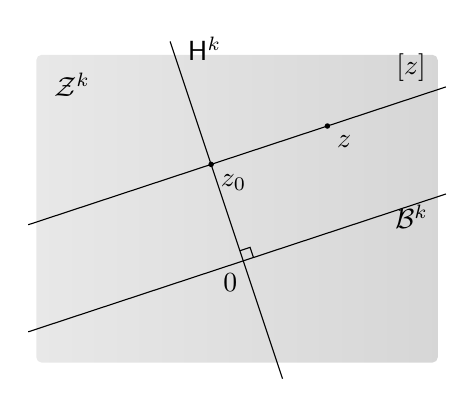
\begin{tikzpicture}[x=.85cm,y=.85cm]
\shade[rounded corners=2pt,left color=gray!18,right color=gray!32] (0,0) rectangle (6,4.6);
\draw (-.12,.4604)--(6.12,2.5196);
\draw (-.12,2.0604)--(6.12,4.1196);
\draw (2,4.8)--(3.68,-.24);
\coordinate (origin) at (3.0931,1.5207);
\coordinate (representative) at (2.6126,2.9622);
\coordinate (cycle) at (4.35,3.5355);
\draw (origin) ++(.1519,.0501)--++(-.0501,.1519)--++(-.1519,-.0501);
\fill (representative) circle (1pt);
\fill (cycle) circle (1pt);
\node[anchor=north east] at (3.15,1.48) {$0$};
\node[anchor=north west] at (representative) {$z_0$};
\node[anchor=north west] at (cycle) {$z$};
\node[anchor=south] at (5.6,4.05) {$[z]$};
\node[anchor=north west] at (.12,4.48) {$\mathcal Z^k$};
\node[anchor=south west] at (2.12,4.37) {$\mathsf H^k$};
\node[anchor=north east] at (6,2.5) {$\mathcal B^k$};
\end{tikzpicture}

\caption{{上边界链空间 $\mathcal B^k$ 是闭上链空间 $\mathcal Z^k$ 的子空间. 上同调空间由闭上链的等价类组成, 其中闭上链 $z$ 的类 $[z]$ 是经过 $z$ 且平行于 $\mathcal B^k$ 的仿射子空间. 每个上同调类 $[z]$ 由属于 $\mathsf H^k$ 的唯一元素 $z_0$ 表示, 它是该类中范数最小的元素.}}\label{fig:cohomology-harmonic-representatives}
\end{figure}

% block: compactness-property-intro page:46 type:ordinary-paragraph
{可利用调和形式得到 Hilbert 复形为 Fredholm 的一个有用判据, 即其同调空间为有限的判据. 空间 $V^k\cap V_k^*\subset W^k$ 配备下述范数后是 Hilbert 空间:}
\[
\|v\|_{V\cap V^*}^2=\|v\|_V^2+\|v\|_{V^*}^2=2\|v\|^2+\|dv\|^2+\|d^*v\|^2.
\]

% block: hilbert-norm-conventions page:46 type:ordinary-paragraph
{这里及下文, 用 $\|\cdot\|_V$ 表示各空间 $V^k$ 中的范数, 用 $\|\cdot\|_{V^*}$ 表示空间 $V_k^*$ 中的范数, 并简单地用 $\|\cdot\|$ 表示空间 $W^k$ 中的范数.}

% block: compactness-property-definition page:46 type:definition

\begin{Definition}\label{def:hilbert-complex-compactness-property}
{若对每个 $k$, 包含映射 $V^k\cap V_k^*\subset W^k$ 都是紧的, 则称 Hilbert 复形具有紧性性质.}
\end{Definition}

% block: compactness-implies-fredholm page:46 type:theorem

\begin{Theorem}\label{thm:compactness-implies-fredholm}
{若 Hilbert 复形具有紧性性质, 则它是闭的且为 Fredholm 复形.}
\end{Theorem}

% block: compactness-closed-range-proof page:46 type:proof
\begin{Proof}
{先验证 $d$ 的像空间是闭的. 设 $T$ 为 $d$ 在 $D(T):=V\cap\mathcal Z^\perp$ 上的限制, 视为无界算子 $W\to W$. 容易验证 $T$ 的像空间与 $d$ 的像空间相同, 且由于 $d$ 是闭算子, $T$ 也闭. 由于 $\mathcal Z^\perp=\overline{\mathcal B}^*\subset\mathcal Z^*\subset V^*$, 有 $D(T)\subset V\cap V^*$, 且 $D(T)$ 上的图范数与 $V\cap V^*$ 范数等价. 由 Theorem~\ref{thm:compact-domain-closed-range}, $T$ 从而 $d$ 均有闭像空间.}

% block: compactness-finite-dimensional-proof page:46 type:proof
{其次注意, 在 $\mathsf H\subset V\cap V^*$ 上, $V\cap V^*$ 范数与 $W$ 范数等价. 因此 $\mathsf H$ 中的闭单位球是紧的, 这意味着 $\mathsf H\cong\mathcal H$ 为有限维, 即该复形是 Fredholm 的.}
\end{Proof}

% block: hodge-decomposition-heading page:46 type:subsection
\subsection{{Hodge 分解}}\label{subsec:hodge-decomposition}

% block: hodge-helmholtz-intro page:46 type:ordinary-paragraph
{Hilbert 复形结构直接导出 Hodge 分解, 它是向量微积分中 Helmholtz 分解的推广.}

% block: cocycle-orthogonal-decomposition page:46 type:ordinary-paragraph
{由于调和 $k$-形式的空间是 $\overline{\mathcal B}^k$ 在 $\mathcal Z^k$ 中的正交补, 立即有}
\begin{equation}\label{eq:cocycle-harmonic-decomposition}
\mathcal Z^k=\overline{\mathcal B}^k\BookOrthSum\mathsf H^k,
\end{equation}

% block: orthogonal-sum-definition page:46 type:ordinary-paragraph
{其中符号 $\BookOrthSum$ 表示正交的和 (注意, 在这一背景下, 无须区分 $W$ 中的正交与 $V$ 中的正交). 由于 $\mathcal Z^k$ 同时是 $W^k$ 和 $V^k$ 的闭子空间, 有}
\[
W^k=\mathcal Z^k\BookOrthSum\mathcal Z^{k\perp}=\mathcal Z^k\BookOrthSum\overline{\mathcal B}_k^*,\qquad V^k=\mathcal Z^k\BookOrthSum\mathcal Z^{k\perp V},
\]
{其中 $\mathcal Z^{k\perp V}=\mathcal Z^{k\perp}\cap V=\overline{\mathcal B}_k^*\cap V$. 结合 \eqref{eq:cocycle-harmonic-decomposition} 得到 Hodge 分解.}

% block: hodge-decomposition-theorem page:47 type:theorem

\begin{Theorem}{Hodge {分解}}\label{thm:hodge-decomposition}
{任意 Hilbert 复形均给出正交分解}
\begin{equation}\label{eq:hodge-base-decomposition}
\begin{tikzpicture}[baseline=(m.base)]
\matrix (m) [matrix of math nodes,ampersand replacement=\&,column sep=6pt,inner sep=0pt] {
W^k={}\&\overline{\mathcal B}^k\&\BookOrthSum\&\mathsf H^k\&\BookOrthSum\&\overline{\mathcal B}_k^*\\};
\draw[decorate,decoration={brace,amplitude=4pt}] ([yshift=6pt]m-1-2.north west)--([yshift=6pt]m-1-4.north east) node[midway,above=5pt] {$\mathcal Z^k=\mathcal B_k^{*\perp}$};
\draw[decorate,decoration={brace,amplitude=4pt}] ([yshift=6pt]m-1-6.north west)--([yshift=6pt]m-1-6.north east) node[midway,above=5pt] {$\mathcal Z^{k\perp}$};
\draw[decorate,decoration={brace,mirror,amplitude=4pt}] ([yshift=-6pt]m-1-2.south west)--([yshift=-6pt]m-1-2.south east) node[midway,below=5pt] {$\mathcal Z_k^{*\perp}$};
\draw[decorate,decoration={brace,mirror,amplitude=4pt}] ([yshift=-6pt]m-1-4.south west)--([yshift=-6pt]m-1-6.south east) node[midway,below=5pt] {$\mathcal Z_k^*=\mathcal B^{k\perp}$};
\end{tikzpicture}
\end{equation}
{以及}
\begin{equation}\label{eq:hodge-domain-decomposition}
V^k=\overline{\mathcal B}^k\BookOrthSum\mathsf H^k\BookOrthSum\mathcal Z^{k\perp V}.
\end{equation}
\end{Theorem}

% block: hodge-closed-complex-description page:47 type:ordinary-paragraph
{对闭 Hilbert 复形, 当然可以去掉边界链空间上的横线. 此时, Hodge 分解说明 $W$ 的每个元素都唯一地分解为 $d$ 的像中的一个元素, $d^*$ 的像中的一个元素以及一个调和形式, 且该分解是正交的.}

% block: poincare-subheading page:47 type:subsection
\subsection{Poincaré {不等式}}\label{subsec:hilbert-poincare-inequality}

% block: poincare-intro page:47 type:ordinary-paragraph
{最后推导的结论是 Poincaré 不等式, 为此必须假设 Hilbert 复形是闭的.}

% block: hilbert-poincare-inequality page:47 type:theorem

\begin{Theorem}{Poincaré {不等式}}\label{thm:hilbert-complex-poincare}
{给定闭 Hilbert 复形, 对每个 $k$, 存在常数 $c_P$, 使得}
\begin{equation}\label{eq:hilbert-poincare-inequality}
\|z\|_V\leq c_P\|dz\|,\qquad z\in\mathcal Z^{k\perp V}.
\end{equation}
\end{Theorem}

% block: hilbert-poincare-proof page:47 type:proof
\begin{Proof}
{由于 Hilbert 复形是闭的, $\mathcal B^{k+1}$ 是 Hilbert 空间. 因而算子 $d^k$ 是 Hilbert 空间 $\mathcal Z^{k\perp V}$ 与 $\mathcal B^{k+1}$ 之间的有界线性同构, 所以它具有有界逆, 由此直接得到 \eqref{eq:hilbert-poincare-inequality}.}
\end{Proof}

% Complete Section 4.3, original PDF 47-49 / printed 37-39.
% block: l2-de-rham-heading page:47 type:section
\section{{Example: $L^2$ de Rham 复形}}\label{sec:l2-de-rham-complex}

% block: l2-de-rham-base-domain page:47 type:ordinary-paragraph
{Hilbert 复形的典型例子是与 Riemannian 流形相伴的 de Rham 复形. 继续讨论 $\mathbb R^3$ 中区域 $\Omega$ 的情形, 并假设其具有 Lipschitz 边界. 基 Hilbert 空间取为 $W^0=W^3=L^2(\Omega)$, $W^1=W^2=L^2(\Omega;\mathbb R^3)$. 算子是 Section~\ref{sec:vector-operators-adjoints} 中讨论的那些算子: $d^0=\operatorname{grad}$, $d^1=\operatorname{curl}$, $d^2=\operatorname{div}$, 定义域分别取为 $H^1$, $H(\operatorname{curl})$ 和 $H(\operatorname{div})$. 那里已看到这些算子是闭的, 因而满足 Hilbert 复形的条件. 由空间 $V^k$ 组成的定义域复形为}
\begin{equation}\label{eq:l2-de-rham-domain-complex}
0\to H^1\xrightarrow{\operatorname{grad}}H(\operatorname{curl})\xrightarrow{\operatorname{curl}}H(\operatorname{div})\xrightarrow{\operatorname{div}}L^2\to0.
\end{equation}

% block: l2-dual-domain-complex page:47 type:ordinary-paragraph
{根据 Section~\ref{sec:vector-operators-adjoints} 中计算的伴随, 对偶复形的定义域复形 (由 $V_k^*$ 组成) 为}
\begin{equation}\label{eq:l2-dual-domain-complex}
0\leftarrow L^2\xleftarrow{-\operatorname{div}}\mathring H(\operatorname{div})\xleftarrow{\operatorname{curl}}\mathring H(\operatorname{curl})\xleftarrow{-\operatorname{grad}}\mathring H^1\leftarrow0.
\end{equation}

% block: de-rham-compactness page:48 type:ordinary-paragraph
{一个重要事实是, $L^2$ de Rham 复形满足紧性性质, 即 $V^k\cap V_k^*$ 紧嵌入 $W^k$. 对 $k=0$, 有 $V^0\cap V_0^*=H^1\cap L^2=H^1$, 由 Rellich 定理, 它在 $W^0=L^2$ 中确实是紧的. $k=3$ 的结论类似. 对 $k=1$ 和 $2$, 所需结论是 $H(\operatorname{curl})\cap\mathring H(\operatorname{div})$ 与 $\mathring H(\operatorname{curl})\cap H(\operatorname{div})$ 在 $L^2(\Omega;\mathbb R^3)$ 中紧. Picard \BookCite{62} 在具有 Lipschitz 边界的 Riemannian 流形这一更一般背景下证明了此结论. 根据 Theorem~\ref{thm:compactness-implies-fredholm}, 紧性性质意味着 de Rham 复形是 Fredholm 的: 各算子的像空间是闭的, 且调和形式空间为有限维. 特别地, 我们已证明 $\operatorname{curl}H(\operatorname{curl})$ 是闭的, 正如 Chapter~\ref{chap:unbounded-operators} 末尾所述. 下面计算调和形式空间, 并给出每个次数上的 Hodge 分解.}

% block: harmonic-zero-forms page:48 type:ordinary-paragraph
{调和 $0$-形式的空间与梯度的零空间 $\mathcal Z^0$ 相同. 这是常数空间, 或者若允许区域有多个连通分支, 则是局部常数空间. 其维数是 $\Omega$ 的连通分支数 $b_0$ (即区域的第零个 Betti 数). 由于空间 $\mathcal B^0=0$, Hodge 分解将 $L^2$ 表示为 $\operatorname{div}\mathring H(\operatorname{div})$ 与常数 (或局部常数) 函数之和.}

% block: harmonic-one-forms pages:48,49 type:ordinary-paragraph
{调和 $1$-形式的空间更复杂. 它由满足 $\operatorname{curl}p=0$, $\operatorname{div}p=0$, 且法向迹 $\gamma_n p$ 在 $\partial\Omega$ 上为零的 $L^2$ 向量场 $p$ 组成. Figure~\ref{fig:de-rham-harmonic-fields} 左图给出了这种函数的一个初等例子, 其区域是环形柱体. 在柱坐标中, 该区域由 $a\leq r\leq b$, $c\leq z\leq d$ 给出, 其中 $0<a<b$, $c<d$, 而调和形式就是 $p=\operatorname{grad}\theta$ 的倍数. 在一般区域上, $\dim\mathsf H^1=b_1$, 即第一个 Betti 数, 它在 Section~\ref{sec:simplicial-chain-complex} 中已定义, 计数贯通区域的隧道数. 对单连通区域, $b_1=0$, Hodge 分解就是经典的 Helmholtz 分解, 将向量场分解为一个梯度 (无旋的, 即旋度为零) 和一个旋度 (螺线的, 即散度为零). 对一般区域, 还必须包含调和部分:}
\[
L^2(\Omega;\mathbb R^3)=\operatorname{grad}H^1(\Omega)\BookOrthSum\operatorname{curl}\mathring H(\operatorname{curl};\Omega)\BookOrthSum\mathsf H^1.
\]

% block: de-rham-harmonic-fields-figure page:48 type:figure
\begin{figure}[htbp]\centering
\includegraphics[page=48,trim=89bp 83bp 57bp 445bp,clip,width=.85\linewidth]{../input/source/Finite Element Exterior Calculus.pdf}
\caption{{左: $\mathbb R^3$ 中环形柱体上的调和 $1$-形式. 右: 球壳上的调和 $2$-形式 (为便于观察, 已切去半个球壳).}}\label{fig:de-rham-harmonic-fields}
\end{figure}

% block: harmonic-two-forms page:49 type:ordinary-paragraph
{调和 $2$-形式的空间同样由无旋且无散的向量场组成, 但此时它们在边界上的切向迹为零. 一个初等例子是在闭球壳 $a<r<b$ 上, 用球坐标给出的 $p=\operatorname{grad}(1/r)$. 见 Figure~\ref{fig:de-rham-harmonic-fields}. 在一般区域上, $\dim\mathsf H^2=b_2$, 即区域中的空腔数. Hodge 分解仍然分解为梯度和旋度, 但边界条件不同, 调和形式空间也不同:}
\[
L^2(\Omega;\mathbb R^3)=\operatorname{grad}\mathring H^1(\Omega)\BookOrthSum\operatorname{curl}H(\operatorname{curl};\Omega)\BookOrthSum\mathsf H^2.
\]

% block: harmonic-three-forms page:49 type:ordinary-paragraph
{最后, 调和 $3$-形式的空间很简单: $\mathsf H^3=0$, 因为 $\mathring H^1$ 中没有梯度为零的非零函数. 当然, $\mathcal B_3^*$ 也为零, 因此 Hodge 分解是平凡的.}

% Complete Section 4.4, original PDF 49-54 / printed 39-44.
% The user-approved non-Fraktur mappings preserve harmonic/cohomology distinctions.
% block: abstract-hodge-heading page:49 type:section
\section{{抽象 Hodge Laplacian}}\label{sec:abstract-hodge-laplacian}

% block: hodge-laplacian-domain-intro page:49 type:ordinary-paragraph
{设 $(W,d)$ 为闭 Hilbert 复形. 与之相伴的是由 $L=dd^*+d^*d$ 给出的次数为 $0$ 的分次算子 $W\to W$. 对与 Riemannian 流形相伴的 de Rham 复形, 此算子称为 Hodge Laplacian; 一般地, 我们将它称为与该复形相伴的 (抽象) Hodge Laplacian. 具体地,}
\begin{equation}\label{eq:abstract-hodge-domain}
D(L^k)=\{\,u\in V^k\cap V_k^*\mid du\in V_{k+1}^*,\ d^*u\in V^{k-1}\,\},
\end{equation}
{且}
\begin{equation}\label{eq:abstract-hodge-operator}
\begin{gathered}
L^k u=d_{k+1}^*d^k u+d^{k-1}d_k^*u=(d^k)^*d^k u+d^{k-1}(d^{k-1})^*u,\qquad u\in D(L^k).
\end{gathered}
\end{equation}

% block: hodge-kernel-identification page:49 type:ordinary-paragraph
{FEEC 的一个主要课题是对给定 $f\in W^k$, 数值求解 Hodge Laplace 方程 $L^k u=f$. 这一问题是否具有唯一解, 取决于调和形式空间 $\mathsf H^k$ 是否为零. 事实上, 下面证明 $L^k$ 的零空间恰好为 $\mathsf H^k$, 由此解释\emph{调和}这一术语. 由 \eqref{eq:harmonic-cocycle-orthogonality} 可知 $\mathsf H^k\subset D(L^k)$, 且对所有 $u\in\mathsf H^k$ 有 $L^k u=0$. 因此 $\mathsf H^k\subset\mathcal N(L^k)$. 另一方面, 由 $L$ 的定义有}
\begin{equation}\label{eq:hodge-green-identity}
\langle L^k u,v\rangle=\langle du,dv\rangle+\langle d^*u,d^*v\rangle,\qquad u\in D(L^k),\ v\in V^k\cap V_k^*.
\end{equation}
{取 $v=u$, 得}
\[
\|du\|^2+\|d^*u\|^2=\langle L^k u,u\rangle,\qquad u\in D(L^k),
\]
{因而,}
\[
\|du\|^2+\|d^*u\|^2=0,
\]
{只要 $u\in\mathcal N(L^k)$. 因此, 若 $u\in\mathcal N(L^k)$, 则 $du$ 与 $d^*u$ 均为零, 从而 $u\in\mathsf H^k$. 这验证了 $\mathcal N(L^k)=\mathsf H^k$, 即 Hodge Laplacian 的解只在相差一个调和形式的意义下确定.}

% block: hodge-solvability-orthogonality page:49 type:ordinary-paragraph
{调和形式还决定了解存在的一个必要条件. 将方程 $L^k u=f$ 与 $q\in\mathsf H^k$ 作内积, 并利用 \eqref{eq:hodge-green-identity}, 得 $\langle f,q\rangle=0$. 因此, 解存在的一个必要条件是正交条件 $f\perp\mathsf H^k$. 事实上, 下面的 Theorem~\ref{thm:hodge-well-posedness} 将证明这一条件不仅必要, 而且足以保证解的存在.}

% block: hodge-three-formulations-heading page:50 type:subsection
\subsection{{Hodge Laplace 问题的三种表述}}\label{subsec:hodge-three-formulations}

% block: hodge-strong-form-intro page:50 type:ordinary-paragraph
{为了构造对任意 $f\in W^k$ 都可解的问题, 利用 $W^k$ 到 $\mathsf H^k$ 上的正交投影 $P_{\mathsf H}$. 由此可提出 Hodge Laplace 方程的如下\emph{强表述}, 我们将证明它是适定的.}

% block: hodge-strong-formulation page:50 type:ordinary-paragraph
\medskip\noindent\textbf{{强表述}}\par
{给定 $f\in W^k$, 求 $u\in D(L^k)$, 使得}
\begin{equation}\label{eq:hodge-strong-formulation}
Lu=f-P_{\mathsf H}f,\qquad u\perp\mathsf H^k.
\end{equation}

% block: hodge-solution-decomposition page:50 type:ordinary-paragraph
{注意, 若 $u$ 为此问题的一个解, 则}
\begin{equation}\label{eq:hodge-data-decomposition}
f=dd^*u+P_{\mathsf H}f+d^*du.
\end{equation}
{显然 $dd^*u\in\mathcal B$, $P_{\mathsf H}f\in\mathsf H$, $d^*du\in\mathcal B^*$, 因而 \eqref{eq:hodge-data-decomposition} 是 $f$ 的 Hodge 分解, 即 $dd^*u=P_{\mathcal B}f$, $d^*du=P_{\mathcal B^*}f$.}

% block: hodge-weak-formulations-intro page:50 type:ordinary-paragraph
{还将考虑该问题的两种弱表述. 原始表述直接对应于强表述.}

% block: hodge-primal-formulation page:50 type:ordinary-paragraph
\medskip\noindent\textbf{{原始弱表述}}\par
{给定 $f\in W^k$, 求 $u\in V^k\cap V_k^*$, 使 $u\perp\mathsf H^k$ 且}
\begin{equation}\label{eq:hodge-primal-formulation}
\langle du,dv\rangle+\langle d^*u,d^*v\rangle=\langle f-P_{\mathsf H}f,v\rangle,\qquad v\in V^k\cap V_k^*.
\end{equation}

% block: hodge-mixed-variables page:50 type:ordinary-paragraph
{对混合弱表述, 引入两个新变量 $\sigma=d^*u\in V^{k-1}$ 和 $p=P_{\mathsf H}f\in\mathsf H^k$.}

% block: hodge-mixed-formulation page:50 type:ordinary-paragraph
\medskip\noindent\textbf{{混合弱表述}}\par
{给定 $f\in W^k$, 求 $\sigma\in V^{k-1}$, $u\in V^k$, $p\in\mathsf H^k$, 使得}
\begin{equation}\label{eq:hodge-mixed-formulation}
\begin{aligned}
\langle\sigma,\tau\rangle-\langle u,d\tau\rangle&=0,&\tau&\in V^{k-1},\\
\langle d\sigma,v\rangle+\langle du,dv\rangle+\langle p,v\rangle&=\langle f,v\rangle,&v&\in V^k,\\
\langle u,q\rangle&=0,&q&\in\mathsf H^k.
\end{aligned}
\end{equation}

% block: hodge-mixed-asymmetry page:50 type:ordinary-paragraph
{一个重要观察是, 与另两种表述不同, 混合弱表述并不对称地处理算子 $d$ 与 $d^*$. 这种表述中只出现算子 $d$, 涉及 $d^*$ 的项以弱形式处理.}

% block: hodge-formulation-equivalence-intro page:50 type:ordinary-paragraph
{尽管形式不同, 这三种表述完全等价.}

% block: hodge-formulation-equivalence page:50 type:theorem

\begin{Theorem}{{表述的等价性}}\label{thm:hodge-formulation-equivalence}
{设 $f\in W^k$. 元素 $u\in W^k$ 是抽象 Hodge Laplace 问题强表述的解, 当且仅当它是原始弱表述的解. 此外, 此时若令 $\sigma=d^*u$, $p=P_{\mathsf H}f$, 则三元组 $(\sigma,u,p)$ 是混合弱表述的解. 最后, 若某个 $(\sigma,u,p)$ 是混合弱表述的解, 则 $u$ 是该问题另两种表述的解, 且 $\sigma=d^*u$, $p=P_{\mathsf H}f$.}
\end{Theorem}

% block: hodge-equivalence-proof-regularity page:51 type:proof
\begin{Proof}
{先证明强表述与原始弱表述的等价性. 若 $u$ 满足强表述, 则当然有 $u\in V\cap V^*$ 且满足原始弱表述. 另一方面, 若 $u$ 满足原始弱表述, 并且\emph{若 $u$ 属于 $D(L)$}, 则它满足强表述. 因此, 需证明任意满足原始弱表述, 从而先验地只属于 $V\cap V^*$ 的 $u$, 实际上属于 \eqref{eq:abstract-hodge-domain} 定义的 $D(L)$, 即满足 $du\in V^*$ 与 $d^*u\in V$. $du\in V^*$ 意味着存在常数 $c$, 使得}
\begin{equation}\label{eq:hodge-du-adjoint-bound}
\langle du,dv\rangle\leq c\|v\|,\qquad v\in V.
\end{equation}

% block: hodge-equivalence-proof-hodge-split page:51 type:proof
{利用 Hodge 分解, 将 $v=v_1+v_2$ 分解, 其中 $v_1\in\mathcal Z$, $v_2\in V\cap\mathcal B^*$. 显然,}
\[
\langle du,dv_1\rangle=0,
\]
{而}
\[
\langle du,dv_2\rangle=\langle du,dv_2\rangle+\langle d^*u,d^*v_2\rangle=\langle f-P_{\mathsf H}f,v_2\rangle\leq c\|v_2\|\leq c\|v\|,
\]
{其中 $c=\|f-P_{\mathsf H}f\|$. 将这些结果相加得到 \eqref{eq:hodge-du-adjoint-bound}, 从而表明 $du\in V^*$. 类似的论证表明 $d^*u\in V$, 因而证明了 $u\in D(L)$, 也就证明原始弱表述的解是强解.}

% block: hodge-equivalence-proof-strong-mixed page:51 type:proof
{其次, 设 $u$ 为强表述的解, 并令 $\sigma=d^*u$, $p=P_{\mathsf H}f$. 由于 $u\in D(L)$, 有 $\sigma\in V$. 混合表述的第一个方程由 $\sigma$ 的定义推出. 由 Hodge Laplace 方程有}
\[
d\sigma+d^*du+p=f,
\]
{与任意 $v\in V$ 作内积, 得到混合方法的第二个方程. 第三个方程由假设 $u\perp\mathsf H^k$ 得到. 这表明 $(\sigma,u,p)$ 是弱表述的解.}

% block: hodge-equivalence-proof-mixed-primal page:51 type:proof
{最后, 若 $(\sigma,u,p)\in V\times V\times\mathsf H$ 是混合弱表述的解, 则第一个方程给出 $u\in V^*$ 和 $d^*u=\sigma$, 最后一个方程给出 $u\perp\mathsf H$. 在第二个方程中取 $v\in\mathsf H$, 可知 $p=P_{\mathsf H}f$. 最后, 在第二个方程中取 $v\in V\cap V^*$, 可得 $u$ 是原始弱表述的解.}
\end{Proof}

% block: hodge-well-posedness-heading page:51 type:subsection
\subsection{{适定性}}\label{subsec:hodge-well-posedness}

% block: hodge-well-posedness-intro page:51 type:ordinary-paragraph
{最后证明, 在计入调和形式之后, 抽象 Hodge Laplace 方程是适定的.}

% block: hodge-well-posedness page:51 type:theorem

\begin{Theorem}{{适定性}}\label{thm:hodge-well-posedness}
{对每个 $f\in W^k$, 存在唯一解 $u\in D(L^k)$, 满足 $u\perp\mathsf H^k$ 且 $Lu=f-P_{\mathsf H}f$. 此外,}
\[
\|u\|+\|du\|+\|d^*u\|+\|dd^*u\|+\|d^*du\|+\|p\|\leq c\|f\|.
\]
{该估计中的常数 $c$ 仅依赖于 Poincaré 不等式 (Theorem~\ref{thm:hilbert-complex-poincare}) 中的常数 $c_P$.}
\end{Theorem}

% block: hodge-well-posedness-proof-reduction page:52 type:proof
\begin{Proof}
{当解存在时, $\|dd^*u\|$, $\|d^*du\|$ 和 $\|p\|$ 的界直接来自 Hodge 分解 $f=dd^*u+d^*du+p$, 因此只须证明对任意 $f\in W$, 存在唯一解且满足}
\[
\|u\|_V+\|d^*u\|\leq c\|f\|.
\]

% block: mixed-hodge-bilinear-form page:52 type:proof
{证明基于混合弱表述. 简记 $X=V^{k-1}\times V^k\times\mathsf H^k$, 将定义混合表述的三个方程的左端合并, 定义有界双线性型 $B:X\times X\to\mathbb R$:}
\begin{equation}\label{eq:hodge-mixed-bilinear-form}
\begin{aligned}
B(\sigma,u,p;\tau,v,q)={}&\langle\sigma,\tau\rangle-\langle u,d\tau\rangle-\langle d\sigma,v\rangle\\
&-\langle du,dv\rangle-\langle p,v\rangle-\langle u,q\rangle.
\end{aligned}
\end{equation}

% block: mixed-hodge-load-functional page:52 type:proof
{注意 $B$ 是对称的. 还通过下式定义有界线性泛函 $F:X\to\mathbb R$:}
\begin{equation}\label{eq:hodge-mixed-load-functional}
F(\tau,v,q)=\langle f,v\rangle.
\end{equation}
{则混合弱表述具有标准形式: 求 $x\in X$, 使得}
\begin{equation}\label{eq:hodge-mixed-abstract-problem}
B(x,y)=F(y),\qquad y\in X.
\end{equation}

% block: hodge-necas-inf-sup page:52 type:proof
{Nečas 对 Lax–Milgram 定理的推广 [\BookNumber{61}, Theorem 3.1] 给出了这一问题何时适定. (对任意 $F\in X'$ 的) 适定性等价于 \emph{inf-sup 条件}}
\begin{equation}\label{eq:hodge-inf-sup-condition}
\gamma:=\inf_{0\ne w\in X}\sup_{0\ne y\in X}\frac{B(w,y)}{\|w\|_X\|y\|_X}>0,
\end{equation}
{此时解 $x$ 满足 $\|x\|_X\leq\gamma^{-1}\|F\|_{X'}$. (一般还需要交换 $w$ 与 $y$ 角色后的第二个 inf-sup 条件, 但本情形中 $B$ 是对称的, 因而不需要.) 下面的定理证明这一 inf-sup 条件.}
\end{Proof}

% block: hodge-inf-sup-theorem page:52 type:theorem

\begin{Theorem}\label{thm:hodge-mixed-inf-sup}
{\eqref{eq:hodge-mixed-bilinear-form} 定义的双线性型 $B$ 满足 inf-sup 条件 \eqref{eq:hodge-inf-sup-condition}, 其中 $\gamma$ 的下界仅依赖于 Poincaré 常数 $c_P$.}
\end{Theorem}

% block: hodge-inf-sup-proof-task page:52 type:proof
\begin{Proof}
{对任意给定的 $(\sigma,u,p)\in V^{k-1}\times V^k\times\mathsf H$, 须构造不恒为零的 $(\tau,v,q)\in V^{k-1}\times V^k\times\mathsf H$, 使得}
\[
B(\sigma,u,p;\tau,v,q)\geq\gamma(\|\sigma\|_V+\|u\|_V+\|p\|)(\|\tau\|_V+\|v\|_V+\|q\|),
\]
{其中 $\gamma$ 仅依赖于 $c_P$. 为此, 使用 Hodge 分解 $u=u_{\mathcal B}+u_{\mathsf H}+u_{\mathcal B^*}$, 其中 $u_{\mathcal B}=P_{\mathcal B}u$, $u_{\mathsf H}=P_{\mathsf H}u$, $u_{\mathcal B^*}=P_{\mathcal B^*}u$. 由于 $u_{\mathcal B}\in\mathcal B^k$, 可写成 $u_{\mathcal B}=d\rho$, 其中 $\rho\in\mathcal Z^{k-1\perp}$. 由 Poincaré 不等式,}
\begin{equation}\label{eq:hodge-inf-sup-lifting-bound}
\|\rho\|_V\leq c_P\|u_{\mathcal B}\|.
\end{equation}

% block: hodge-inf-sup-test-choice page:52 type:proof
{然后定义}
\begin{equation}\label{eq:hodge-inf-sup-test-choice}
\begin{gathered}
\tau=\sigma-\frac{1}{c_P^2}\rho\in V^{k-1},\qquad v=-u-d\sigma-p\in V^k,\\
q=-p+u_{\mathsf H}\in\mathsf H^k.
\end{gathered}
\end{equation}

% block: hodge-inf-sup-test-bound page:53 type:proof
{由 \eqref{eq:hodge-inf-sup-lifting-bound} 及 Hodge 分解的正交性, 有}
\begin{equation}\label{eq:hodge-inf-sup-test-bound}
\|\tau\|_V+\|v\|_V+\|q\|\leq C(\|\sigma\|_V+\|u\|_V+\|p\|).
\end{equation}
{将 \eqref{eq:hodge-inf-sup-test-choice} 代入 \eqref{eq:hodge-mixed-bilinear-form}, 得}
\[
\begin{aligned}
B(\sigma,u,p;\tau,v,q)={}&\|\sigma\|^2+\|d\sigma\|^2+\|du\|^2+\|p\|^2+\|u_{\mathsf H}\|^2\\
&+\frac{1}{c_P^2}\|u_{\mathcal B}\|^2-\frac{1}{c_P^2}\langle\sigma,\rho\rangle.
\end{aligned}
\]

% block: hodge-inf-sup-cross-term page:53 type:proof
{利用 Cauchy–Schwarz 不等式, 代数-几何平均不等式以及 \eqref{eq:hodge-inf-sup-lifting-bound} 估计最后一项:}
\[
\begin{aligned}
\langle\sigma,\rho\rangle&\leq\|\sigma\|\|\rho\|\leq\frac{c_P^2}{2}\|\sigma\|^2+\frac{1}{2c_P^2}\|\rho\|^2\\
&\leq\frac{c_P^2}{2}\|\sigma\|^2+\frac12\|u_{\mathcal B}\|^2.
\end{aligned}
\]
{因此}
\[
\begin{aligned}
B(\sigma,u,p;\tau,v,q)\geq{}&\frac12\|\sigma\|^2+\|d\sigma\|^2+\|du\|^2+\|p\|^2\\
&+\|u_{\mathsf H}\|^2+\frac{1}{2c_P^2}\|u_{\mathcal B}\|^2.
\end{aligned}
\]

% block: hodge-inf-sup-dual-boundary-bound page:53 type:proof
{现对 $u_{\mathcal B^*}$ 应用 Poincaré 不等式, 其中 $du_{\mathcal B^*}=du$:}
\[
\|u_{\mathcal B^*}\|_V\leq c_P\|du\|.
\]
{得到}
\[
\begin{aligned}
&B(\sigma,u,p;\tau,v,q)\\
&\geq\frac12\|\sigma\|^2+\|d\sigma\|^2+\frac12\|du\|^2+\|p\|^2+\|u_{\mathsf H}\|^2\\
&\qquad+\frac{1}{2c_P^2}\|u_{\mathcal B}\|^2+\frac{1}{2c_P^2}\|u_{\mathcal B^*}\|^2\\
&\geq\eta(\|\sigma\|^2+\|d\sigma\|^2+\|u_{\mathcal B}\|^2+\|u_{\mathsf H}\|^2+\|u_{\mathcal B^*}\|^2+\|du\|^2+\|p\|^2)\\
&=\eta(\|\sigma\|_V^2+\|u\|_V^2+\|p\|^2),
\end{aligned}
\]
{其中 $\eta=\min(1/2,1/2c_P^2)$ 仅依赖于 $c_P$. 由此界及 \eqref{eq:hodge-inf-sup-test-bound}, 容易得到 inf-sup 条件.}
\end{Proof}

% block: hodge-general-load-remark page:53 type:remark

\begin{Remark}\label{rem:hodge-general-mixed-load}
{Theorem~\ref{thm:hodge-mixed-inf-sup} 中的 inf-sup 条件意味着混合问题 \eqref{eq:hodge-mixed-abstract-problem} 对一般 $F\in X'$ 适定, 而不仅对具有 \eqref{eq:hodge-mixed-load-functional} 形式的 $F$ 适定.}
\end{Remark}

% block: hodge-solution-operator page:53 type:ordinary-paragraph
{已确立 Hodge Laplacian 的适定性, 将解算子记为 $K$. 即对 $f\in W$, 通过方程 $LKf=f-P_{\mathsf H}f$, $Kf\perp\mathsf H$ 定义 $Kf\in D(L)$. 用 $K$ 表示, 混合表述的解由 $\sigma=d^*Kf$, $u=Kf$, $p=P_{\mathsf H}f$ 给出. 因而 Hodge 投影为 $P_{\mathcal B}=dd^*K$, $P_{\mathcal B^*}=d^*dK$, 且}
\[
u=dd^*Ku+P_{\mathsf H}u+d^*dKu,\qquad u\in W.
\]

% block: hodge-mixed-choice-remark page:53 type:remark

\begin{Remark}\label{rem:hodge-mixed-discretization-motivation}
{读者可能会问, 为什么选择用混合表述而非原始弱表述来确立抽象 Hodge Laplacian 的适定性. 毕竟, 原始表述的双线性型由 Poincaré 不等式可知是强制的, 因此可以应用 Riesz 表示定理, 无须验证 inf-sup 条件. 原因在于我们着眼于 Hodge Laplacian 的离散化, 这将是下一章的主题. 离散化将基于混合表述, 正如将要看到的, 混合表述远比原始表述更适于离散化. 混合双线性型的 inf-sup 条件 (而不仅是对具有 \eqref{eq:hodge-mixed-load-functional} 形式的 $F$ 的适定性) 届时将成为离散化方法分析的关键.}
\end{Remark}

% block: boundary-problems-heading page:54 type:subsection
\subsection{{$\mathcal B$ 与 $\mathcal B^*$ 问题}}\label{subsec:boundary-coboundary-problems}

% block: boundary-problem-hodge-reduction page:54 type:ordinary-paragraph
{本小节考察数据 $g$ 属于 $\mathcal B$ 或 $\mathcal B^*$ 时的 Hodge Laplace 方程 $Lv=g$. 前一情形中, 对某个 $f\in V$ 有 $g=df$ (若 $g\in V^k$, 则 $f\in V^{k-1}$). 由 Hodge Laplace 方程}
\begin{equation}\label{eq:hodge-boundary-problem-potential}
Lu=f-P_{\mathsf H}f
\end{equation}
{在数据为 $f$ 时的解 $u$, 令 $v=du$ 即得到 $Lv=g$ 的解. 这是合理的, 因为形式上有}
\[
Lv=(dd^*+d^*d)du=dd^*du=d(dd^*+d^*d)u=d(f-P_{\mathsf H}f)=g.
\]

% block: boundary-problem-domain-justification page:54 type:ordinary-paragraph
{只要 $v=du\in D(L)$, 这一形式计算就有依据. 为说明这一点, 注意由于 $u\in D(L)$, 有 $v=du\in V^*$ 且 $v\in V$. 此外 $dv=0$, 并且由 $f\in V$ 及 $\mathcal Z\subset V$, 有 $d^*v=d^*du=P_{\mathcal B^*}f=f-P_{\mathcal Z}f\in V$. 这就表明 $v\in D(L)$, 如前所述.}

% block: boundary-problem-intro page:54 type:ordinary-paragraph
{因此, 当 Hodge Laplacian 的数据 $g$ 属于 $\mathcal B$ 时, 相应解 $v$ 也属于 $\mathcal B$. 此时 Hodge Laplacian 中的项 $d^*dv$ 为零, 所以 $v$ 满足另一个问题.}

% block: boundary-problem-formulation page:54 type:ordinary-paragraph
\medskip\noindent\textbf{{$\mathcal B$ 问题}}\par
{给定 $g\in\mathcal B^k$, 求 $v\in\mathcal B^k$, 使 $dd^*v=g$.}

% block: boundary-problem-equivalence page:54 type:ordinary-paragraph
{按定义, 此问题的解还必须属于 $D(dd^*)=\{\,v\in V_k^*\mid d^*v\in V^{k-1}\,\}$. 刚才已看到, 对 $g\in\mathcal B^k$, 若 $v$ 是数据为 $g$ 的 Hodge Laplace 问题的解, 则 $v$ 是 $\mathcal B$ 问题的解. 反之, 若 $v$ 是 $\mathcal B$ 问题的解, 则有 $dv=0$, 从而 $Lv=dd^*v=g$, 即 $v$ 是 Hodge Laplace 问题的解. 由 Hodge Laplace 问题的适定性, 得到 $\mathcal B$ 问题的适定性 (但仅对 $g\in\mathcal B^k$; 否则无解).}

% block: boundary-problem-well-posedness page:54 type:theorem

\begin{Theorem}\label{thm:hodge-boundary-problem}
{若 $g\in\mathcal B^k$, 则数据为 $g$ 的 $\mathcal B$ 问题具有唯一解 $v$, 且此解与相同数据的 Hodge Laplace 问题的唯一解相同.}
\end{Theorem}

% block: dual-boundary-problem-intro page:54 type:ordinary-paragraph
{当然, 对 $d^*$ 也有类似结论: 若 $f\in V^*$, 且 $u$ 为相应 Hodge Laplace 问题的解, 则 $v=d^*u\in D(L)$, 并且它是数据为 $g=d^*f$ 的 Hodge Laplace 问题的解. 此外, 若 $g\in\mathcal B^*$, 则它也是下述问题的唯一解.}

% block: dual-boundary-problem-formulation page:54 type:ordinary-paragraph
\medskip\noindent\textbf{{$\mathcal B^*$ 问题}}\par
{给定 $g\in\mathcal B_k^*$, 求 $v\in\mathcal B_k^*$, 使 $d^*dv=g$.}

% Complete Section 4.5 and Box 4.1, original PDF 54-60 / printed 44-50.
% The printed signs and the last summand in Box 4.1 are retained, not corrected.
% block: hodge-r3-heading page:54 type:section
\section{{Example: $\mathbb R^3$ 中的 Hodge Laplacian}}\label{sec:hodge-r3}

% block: hodge-r3-introduction pages:54,55 type:ordinary-paragraph
{现在回到我们贯穿使用的例子, 即 $\mathbb R^3$ 中具有 Lipschitz 边界的区域上的 de Rham 复形. 在 Section~\ref{sec:l2-de-rham-complex} 中已看到, 它构成闭 Hilbert 复形. 因此, 对每个 $k=0,1,2,3$, 都得到与该复形相伴的 Hodge Laplace 问题, 它是一个适定的偏微分方程边值问题. 为了解释这些问题, 只需解释空间 $V^k$ 和 $V_k^*$ 以及算子 $d^k$ 和 $d_k^*$; 为此我们将频繁使用定义域复形 \eqref{eq:l2-de-rham-domain-complex} 及对偶定义域复形 \eqref{eq:l2-dual-domain-complex}.}

% block: hodge-r3-k0-heading page:55 type:subsection
\subsection{$k=0$}\label{subsec:hodge-r3-k0}

% block: hodge-r3-k0-domain page:55 type:ordinary-paragraph
{假设区域连通, 则调和形式空间 $\mathsf H^0$ 仅由常数构成, 且 $P_{\mathsf H}f=\bar f$, 即 $f$ 在 $\Omega$ 上的平均值. 由于 $d_0^*=0$, 有 $L^0u=(dd^*+d^*d)u=d^*du=-\operatorname{div}\operatorname{grad}u=-\Delta u$, 定义域为}
\[
\begin{aligned}
D(L)&=\{\,u\in H^1(\Omega)\mid\operatorname{grad}u\in\mathring H(\operatorname{div},\Omega)\,\}\\
&=\{\,u\in H^1(\Omega)\mid\Delta u\in L^2(\Omega),\ \partial u/\partial n=0\text{ on }\partial\Omega\,\},
\end{aligned}
\]
{其中 $\Delta$ 表示通常的 Laplacian $\Delta=\sum_{i=1}^3\partial^2/\partial x_i^2$. 给定 $f\in L^2(\Omega)$, 强表述 \eqref{eq:hodge-strong-formulation} 就是求 $u\in H^1$, 使得}
\begin{equation}\label{eq:hodge-r3-neumann-strong}
-\Delta u=f-\bar f\text{ in }\Omega,\qquad\frac{\partial u}{\partial n}=0\text{ on }\partial\Omega,\qquad\int u=0.
\end{equation}

% block: hodge-r3-neumann-interpretation page:55 type:ordinary-paragraph
{因此, 与 de Rham 复形相伴的 $k=0$ Hodge Laplace 问题, 就是 Poisson 方程通常的 Neumann 问题; 减去 $\bar f$ 的调整是为了使数据 $f$ 与齐次 Neumann 边界条件相容.}

% block: hodge-r3-neumann-weak page:55 type:ordinary-paragraph
{接下来讨论原始和混合弱表述. 由于 $V^{-1}=0$, 当 $k=0$ 时, 混合弱表述 \eqref{eq:hodge-mixed-formulation} 中的 $\sigma$ 和 $\tau$ 均消失. 因此在 $k=0$ 时两种弱表述没有区别. 它们都是求 $u\in H^1$, 使得}
\begin{equation}\label{eq:hodge-r3-neumann-weak}
\int\operatorname{grad}u\cdot\operatorname{grad}v=\int(f-\bar f)v,\qquad v\in H^1,\qquad\int_\Omega u=0.
\end{equation}

% block: hodge-r3-neumann-equivalence page:55 type:ordinary-paragraph
{由 Theorem~\ref{thm:hodge-formulation-equivalence} 已知, 此问题等价于强表述问题 \eqref{eq:hodge-r3-neumann-strong}. 为使讨论具体, 现在直接验证 \eqref{eq:hodge-r3-neumann-weak} 蕴含 \eqref{eq:hodge-r3-neumann-strong}, 另一个方向更容易. 在 \eqref{eq:hodge-r3-neumann-weak} 中取 $v\in C_0^\infty(\Omega)$, 可见}
\begin{equation}\label{eq:hodge-r3-neumann-distribution}
-\operatorname{div}\operatorname{grad}u=f-\bar f
\end{equation}
{在分布意义下成立, 因此由 $f\in L^2$ 可知, $\operatorname{grad}u$ 属于 $H(\operatorname{div})$. 故可在分部积分公式 \eqref{eq:normal-trace-green} 中取 $w=\operatorname{grad}u$, 再利用 \eqref{eq:hodge-r3-neumann-weak} 和 \eqref{eq:hodge-r3-neumann-distribution}, 得到}
\[
\langle\gamma_n(\operatorname{grad}u),\operatorname{tr}v\rangle=\int(\operatorname{div}\operatorname{grad}u)v+\int\operatorname{grad}u\cdot\operatorname{grad}v=0,\quad v\in H^1.
\]
{由于 $\operatorname{tr}v$ 可以是 $H^{1/2}(\partial\Omega)$ 的任意元素, 可知 $\gamma_n(\operatorname{grad}u)=0$, 即边界上有 $\partial u/\partial n=0$. 注意, 在弱表述中, 边界条件是\emph{自然}施加的, 即通过分部积分由方程蕴含, 而不是施加在求解 $u$ 所在的空间中.}

% block: hodge-r3-k0-boundary-problems page:55 type:ordinary-paragraph
{再看 $\mathcal B$ 和 $\mathcal B^*$ 问题, 由于 $\mathcal B^0=0$, 并没有新的内容. 因此, 在 $k=0$ 时不存在 $\mathcal B$ 问题, 而 $\mathcal B^*$ 问题本质上就是完整的 Hodge Laplacian 问题.}

% block: hodge-r3-k0-summary page:56 type:ordinary-paragraph
{概括 $k=0$ 的情形, $0$-形式的 Hodge Laplacian 就是 Poisson 方程的 Neumann 问题. 此时原始和混合弱表述一致, 都是 Neumann 问题的标准弱表述, 其中边界条件是\emph{自然}施加的.}

% block: hodge-r3-k1-heading page:56 type:subsection
\subsection{$k=1$}\label{subsec:hodge-r3-k1}

% block: hodge-r3-k1-strong page:56 type:ordinary-paragraph
{$k=1$ 的情形更有意思. 调和形式空间 $\mathsf H^1$ 是向量场空间, 其维数为 $b_1$, 即第一个 Betti 数. 强表述是求 $u\in H(\operatorname{curl})\cap\mathring H(\operatorname{div})$, 满足 $\operatorname{curl}u\in\mathring H(\operatorname{curl})$, $\operatorname{div}u\in H^1$, 以及偏微分方程}
\begin{equation}\label{eq:hodge-r3-vector-laplace}
\operatorname{curl}\operatorname{curl}u-\operatorname{grad}\operatorname{div}u=f-P_{\mathsf H}f\text{ in }\Omega.
\end{equation}
{注意, 微分算子 $\operatorname{curl}\operatorname{curl}-\operatorname{grad}\operatorname{div}$ 是负的向量 Laplacian $-\vec\Delta$, 因为对光滑向量场有 \[\operatorname{curl}\operatorname{curl}u-\operatorname{grad}\operatorname{div}u=(-\Delta u_1,-\Delta u_2,-\Delta u_3)\] 其中 $u=(u_1,u_2,u_3)$.}

% block: hodge-r3-magnetic-boundary page:56 type:ordinary-paragraph
{定义域 $D(L^1)$ 的定义蕴含边界条件}
\begin{equation}\label{eq:hodge-r3-magnetic-boundary}
u\cdot n=0,\qquad(\operatorname{curl}u)\times n=0\text{ on }\partial\Omega,
\end{equation}
{当然, 还需要附加条件 $u\perp\mathsf H^1$ 来保证唯一性. 条件 \eqref{eq:hodge-r3-magnetic-boundary} 有时称为\emph{磁边界条件}, 其原因将在 Section~\ref{sec:maxwell-equations} 讨论 Maxwell 方程时变得更清楚.}

% block: hodge-r3-k1-primal page:56 type:ordinary-paragraph
{原始弱表述是求 $u\in H(\operatorname{curl})\cap\mathring H(\operatorname{div})$, 使得}
\begin{equation}\label{eq:hodge-r3-magnetic-primal}
\begin{gathered}
\langle\operatorname{curl}u,\operatorname{curl}v\rangle+\langle\operatorname{div}u,\operatorname{div}v\rangle=\langle f-P_{\mathsf H}f,v\rangle,\\
v\in H(\operatorname{curl})\cap\mathring H(\operatorname{div}).
\end{gathered}
\end{equation}
{注意, 在此表述中, 边界条件 $u\cdot n=0$ 是本质的 (施加在求解 $u$ 所在的空间中), 而条件 $\operatorname{curl}u\times n=0$ 是自然的.}

% block: hodge-r3-k1-mixed page:56 type:ordinary-paragraph
{相比之下, 混合弱表述是求 $\sigma\in H^1$, $u\in H(\operatorname{curl})$, $p\in\mathsf H^1$, 不施加任何边界条件, 并满足}
\begin{equation}\label{eq:hodge-r3-magnetic-mixed}
\begin{aligned}
\int\sigma\tau-\int u\cdot\operatorname{grad}\tau&=0,&\tau&\in H^1,\\
\int\operatorname{grad}\sigma\cdot v+\int\operatorname{curl}u\cdot\operatorname{curl}v+\int p\cdot v&=\int f\cdot v,&v&\in H(\operatorname{curl}),\\
\int u\cdot q&=0,&q&\in\mathsf H^1.
\end{aligned}
\end{equation}
{在此表述中, 边界条件 \eqref{eq:hodge-r3-magnetic-boundary} 都是自然的, 分别来自第一个和第二个方程中的分部积分. 注意, 除未知向量场 $u$ 外, 此表述还以标量函数 $\sigma=-\operatorname{div}u$ 为第二个未知量 (当然还有 $p=P_{\mathsf H}f$).}

% block: hodge-r3-k1-b-problem page:56 type:ordinary-paragraph
{当 $f\in\mathcal B^1$, 即 $f$ 为梯度时, 解 $u$ 也是梯度, 这可以表述为 $\operatorname{curl}u=0$ 且 $u\perp\mathsf H^1$. 因此 $\mathcal B^1$ 问题是求 $u$, 使得}
\[
-\operatorname{grad}\operatorname{div}u=f,\ \operatorname{curl}u=0\text{ in }\Omega,\qquad u\cdot n=0\text{ on }\partial\Omega,\qquad u\perp\mathsf H^1.
\]

% block: hodge-r3-div-curl-application page:57 type:ordinary-paragraph
{由抽象理论可知, 对 $f\in\mathcal B^1$, 此问题具有唯一解; 而且, 可通过对同一 $f$ 求解完整的 Hodge Laplacian 问题 (例如通过混合弱表述) 来计算此解. 此类问题的一个应用是求解 div-curl 问题}
\[
\operatorname{div}u=F,\qquad\operatorname{curl}u=0,
\]
{这可以通过取 $f=\operatorname{grad}F$ 实现 (为与 $u$ 的边界条件相容, 需要 $\int F=0$).}

% block: hodge-r3-k1-bstar-problem page:57 type:ordinary-paragraph
{另一方面, 当 $f\in\mathcal B_1^*$, 即 $f\in\operatorname{curl}\mathring H(\operatorname{curl})$ 时, 就得到 $\mathcal B^*$ 问题. 此时 $u$ 由下式确定:}
\[
\begin{gathered}
\operatorname{curl}\operatorname{curl}u=f,\ \operatorname{div}u=0\text{ in }\Omega,\\
u\cdot n=0,\ \operatorname{curl}u\times n=0\text{ on }\partial\Omega,\qquad u\perp\mathsf H^1.
\end{gathered}
\]
{这种 curl-curl 问题出现在电磁学中. 同样, 可通过求解完整的 Hodge Laplace 问题来确定其解.}

% block: hodge-r3-k2-heading page:57 type:subsection
\subsection{$k=2$}\label{subsec:hodge-r3-k2}

% block: hodge-r3-k2-domain page:57 type:ordinary-paragraph
{此情形仍得到向量 Laplace 方程 \eqref{eq:hodge-r3-vector-laplace}, 但边界条件不同 (调和形式也不同, 其中 $\dim\mathsf H^2=b_2$). $L^2$ 的定义域由满足 $\operatorname{div}u\in\mathring H^1$ 和 $\operatorname{curl}u\in H(\operatorname{curl})$ 的 $u\in H(\operatorname{div})\cap\mathring H(\operatorname{curl})$ 构成. 因此得到\emph{电边界条件}:}
\[
u\times n=0,\ \operatorname{div}u=0\text{ on }\partial\Omega.
\]

% block: hodge-r3-k2-mixed page:57 type:ordinary-paragraph
{这些条件中, 第一个在原始变分表述中是本质的, 第二个是自然的. 当然, 在混合弱表述中两者都是自然的; 该表述是求 $\sigma\in H(\operatorname{curl})$, $u\in H(\operatorname{div})$, $p\in\mathsf H^2$, 使得}
\begin{equation}\label{eq:hodge-r3-electric-mixed}
\begin{aligned}
\int\sigma\cdot\tau-\int u\cdot\operatorname{curl}\tau&=0,&\tau&\in H(\operatorname{curl}),\\
\int\operatorname{curl}\sigma\cdot v+\int\operatorname{div}u\operatorname{div}v+\int p\cdot v&=\int f\cdot v,&v&\in H(\operatorname{div}),\\
\int u\cdot q&=0,&q&\in\mathsf H^2.
\end{aligned}
\end{equation}
{注意, 此表述与 $k=1$ 时的混合弱表述 \eqref{eq:hodge-r3-magnetic-mixed} 很不相同. 这里的附加场 $\sigma$ 是向量场, 而在 $k=1$ 时它是标量场.}

% block: hodge-r3-k2-boundary-problems page:57 type:ordinary-paragraph
{当 $k=2$ 时, $\mathcal B$ 问题为}
\[
\operatorname{curl}\operatorname{curl}u=f,\ \operatorname{div}u=0\text{ in }\Omega,\qquad u\times n=0,\text{ on }\partial\Omega,\qquad u\perp\mathsf H^2,
\]
{若 $f\in\operatorname{curl}H(\operatorname{curl})$, 则它具有唯一解. $\mathcal B_2^*$ 问题为}
\[
\begin{gathered}
-\operatorname{grad}\operatorname{div}u=f,\ \operatorname{curl}u=0\text{ in }\Omega,\\
u\times n=0,\ \operatorname{div}u=0\text{ on }\partial\Omega,\qquad u\perp\mathsf H^2,
\end{gathered}
\]
{对 $f\in\operatorname{grad}\mathring H^1$ 可解. 注意, $\mathcal B^2$ 问题的微分方程与 $\mathcal B_1^*$ 问题的微分方程一致, $\mathcal B_2^*$ 问题的微分方程与 $\mathcal B^1$ 问题的微分方程一致, 但相应的边界条件并不相同.}

% block: hodge-r3-table page:58 type:table
\begin{table}[htbp]\centering\small
\caption{{de Rham 复形的 Hodge Laplace 问题. $\sigma$ 是混合弱表述中的附加变量. 带下划线的边界条件 (不涉及导数的那些条件) 在原始弱表述中是本质的, 其余是自然的. 所有边界条件在混合弱表述中都是自然的.}}\label{tab:hodge-r3-boundary-conditions}
\setlength{\tabcolsep}{4pt}
\begin{tabular}{cccll}\hline
$k$&$L^k$&$\sigma$&{边界条件}&{调和形式}\\\hline
$0$&$-\Delta$&$0$&Neumann: $\partial u/\partial n=0$&$\mathsf H^0$ $(\dim b_0)$\\\noalign{\vskip4pt}
$1$&$-\vec\Delta$&$-\operatorname{div}u$&{磁}: $\underline{u\cdot n=0}$, $\operatorname{curl}u\times n=0$&$\mathsf H^1$ $(\dim b_1)$\\\noalign{\vskip4pt}
$2$&$-\vec\Delta$&$\operatorname{curl}u$&{电}: $\underline{u\times n=0}$, $\operatorname{div}u=0$&$\mathsf H^2$ $(\dim b_2)$\\\noalign{\vskip4pt}
$3$&$-\Delta$&$-\operatorname{grad}u$&Dirichlet: $\underline{u=0}$&$\mathsf H^3=0$\\\hline
\end{tabular}
\end{table}

% block: hodge-r3-k3-heading page:58 type:subsection
\subsection{$k=3$}\label{subsec:hodge-r3-k3}

% block: hodge-r3-k3-dirichlet page:58 type:ordinary-paragraph
{空间 $\mathcal B_3^*$ 和 $\mathsf H^3$ 都为零. Laplacian 的定义域为 $D(L^3)=\{\,u\in\mathring H^1\mid\Delta u\in L^2\,\}$, 因此该边值问题就是 Poisson 方程的 Dirichlet 问题:}
\[
-\Delta u=f\text{ in }\Omega,\qquad u=0\text{ on }\partial\Omega.
\]
{其原始弱表述是显然的: 求 $u\in\mathring H^1$, 使得}
\[
\int\operatorname{grad}u\cdot\operatorname{grad}v=\int fv,\qquad v\in\mathring H^1.
\]
{混合弱表述是求 $\sigma\in H(\operatorname{div})$, $u\in L^2$, 使得}
\[
\begin{gathered}
\int\sigma\cdot\tau-\int u\operatorname{div}\tau=0,\qquad\tau\in H(\operatorname{div}),\\
\int\operatorname{div}\sigma\,v=\int fv,\qquad v\in L^2.
\end{gathered}
\]
{在混合表述中, Dirichlet 条件是自然的.}

% block: hodge-r3-table-summary page:58 type:ordinary-paragraph
{Table~\ref{tab:hodge-r3-boundary-conditions} 汇集了 de Rham 复形的 Hodge Laplacian 问题的主要特征.}

% block: hodge-r3-boundary-duality-heading page:58 type:subsection
\subsection{{带边界条件的 de Rham 复形与对偶性}}\label{subsec:de-rham-boundary-duality}

% block: hodge-r3-boundary-complex page:58 type:ordinary-paragraph
{刚才讨论了抽象理论在 $L^2$ de Rham 复形中的应用, 其定义域复形由 \eqref{eq:l2-de-rham-domain-complex} 给出. 也可以将理论应用于\emph{带边界条件的 $L^2$ de Rham 复形}, 即基空间仍为 $L^2$, 而定义域复形为下式的 Hilbert 复形:}
\[
0\to\mathring H^1\xrightarrow{\operatorname{grad}}\mathring H(\operatorname{curl})\xrightarrow{\operatorname{curl}}\mathring H(\operatorname{div})\xrightarrow{\operatorname{div}}L^2\to0.
\]
{除若干符号和指标的变化外, 此 Hilbert 复形本质上就是 \eqref{eq:l2-de-rham-domain-complex} 的对偶复形, 即 \eqref{eq:l2-dual-domain-complex}. 具体地, 带边界条件的 de Rham 复形中指标为 $k$ 的空间, 就是原 de Rham 复形的对偶复形中指标为 $3-k$ 的空间. 因此, 带边界条件的 de Rham 复形的对偶复形为}
\[
0\leftarrow L^2\xleftarrow{-\operatorname{div}}H(\operatorname{div})\xleftarrow{\operatorname{curl}}H(\operatorname{curl})\xleftarrow{-\operatorname{grad}}H^1\leftarrow0,
\]
{即除符号和指标外, 就是原 de Rham 复形.}

% block: hodge-r3-boundary-table page:59 type:table
\begin{table}[htbp]\centering\small
\caption{{带边界条件的 de Rham 复形的 Hodge Laplace 问题. 在混合表述中, 所有边界条件都是本质的; 在原始表述中, 带下划线的边界条件是本质的. 见 Table~\ref{tab:hodge-r3-boundary-conditions}.}}\label{tab:hodge-r3-relative-boundary-conditions}
\setlength{\tabcolsep}{3pt}
\begin{tabular}{cccll}\hline
$k$&$L^k$&$\sigma$&{边界条件}&{调和形式}\\\hline
$0$&$-\Delta$&$0$&Dirichlet: $\underline{u=0}$&$\mathring{\mathsf H}^0=0$\\\noalign{\vskip4pt}
$1$&$-\vec\Delta$&$-\operatorname{div}u$&{电}: $\underline{u\times n=0}$, $\operatorname{div}u=0$&$\mathring{\mathsf H}^1=\mathsf H^2$ $(\dim b_2)$\\\noalign{\vskip4pt}
$2$&$-\vec\Delta$&$\operatorname{curl}u$&{磁}: $\underline{u\cdot n=0}$, $\operatorname{curl}u\times n=0$&$\mathring{\mathsf H}^2=\mathsf H^1$ $(\dim b_1)$\\\noalign{\vskip4pt}
$3$&$-\Delta$&$-\operatorname{grad}u$&Neumann: $\partial u/\partial n=0$&$\mathring{\mathsf H}^3=\mathsf H^0$ $(\dim b_0)$\\\hline
\end{tabular}
\end{table}

% block: hodge-r3-poincare-lefschetz page:59 type:ordinary-paragraph
{若用 $\mathring{\mathcal B}^k$, $\mathring{\mathcal Z}^k$ 和 $\mathring{\mathsf H}^k$ 表示带边界条件的复形的边界空间, 闭链空间和调和形式空间, 则有 $\mathring{\mathcal B}^k=\mathcal B^{3-k}$, 对 $\mathcal Z$ 和 $\mathsf H$ 也有类似关系. (在 $n$ 维流形上的关系 $\mathsf H^{n-k}=\mathring{\mathsf H}^k$ 称为 \emph{Poincaré–Lefschetz 对偶性}. 对无边界流形, 它成为 $\mathsf H^{n-k}=\mathsf H^k$, 即 Poincaré 对偶性.) 容易验证, 除指标变化外, 带边界条件的复形的强表述和原始弱表述与通常的 de Rham 复形的相应表述一致, 因而得到与上面相同的边值问题. 例如 $k=0$ 的问题就是带 Dirichlet 边界条件的 Poisson 方程. 然而, 对 $k>0$ 的问题, 混合弱表述带来了新的内容. 例如当 $k=1$ 时, 求 $\sigma\in\mathring H^1$, $u\in\mathring H(\operatorname{curl})$, $p\in\mathring{\mathsf H}^1=\mathsf H^2$, 使得}
\[
\begin{aligned}
\int\sigma\tau-\int u\cdot\operatorname{grad}\tau&=0,&\tau&\in\mathring H^1,\\
\int\operatorname{grad}\sigma\cdot v+\int\operatorname{curl}u\cdot\operatorname{curl}v+\int p\cdot v&=\int f\cdot v,&v&\in\mathring H(\operatorname{curl}).\\
\int u\cdot q&=0,&q&\in\mathsf H^2.
\end{aligned}
\]

% block: hodge-r3-relative-mixed-comparison page:59 type:ordinary-paragraph
{这是向量 Laplacian 在边界条件 $\operatorname{div}u=0$, $u\times n=0$ 下的混合表述. 这些边界条件与通常的 de Rham 复形中 $k=2$ 问题的边界条件相同. 但是, 那个问题的混合方法 \eqref{eq:hodge-r3-electric-mixed} 完全不同, 辅助变量 $\sigma$ 使用向量场而不是这里的标量场, 并且边界条件是自然施加的, 而不是像这里这样作为本质条件施加.}

% block: hodge-r3-relative-summary page:59 type:ordinary-paragraph
{对 $k=2$ 和 $k=3$ 也有类似情形, 细节留待读者推导. Table~\ref{tab:hodge-r3-relative-boundary-conditions} 给出了汇总.}

% block: hilbert-summary-heading page:60 type:ordinary-paragraph
\begin{MBSourceBox}
\refstepcounter{booksummary}\label{box:hilbert-complexes-summary}
\noindent\textbf{Box~\thebooksummary:} {Chapter~\ref{chap:hilbert-complexes} Hilbert 复形内容摘要.}\par

% block: hilbert-summary-definition page:60 type:ordinary-paragraph
{\emph{Hilbert 复形}是由 Hilbert 空间 $W^k$ 以及从一个空间到下一个空间的稠定闭算子 $d^k$ 构成的序列, 其中 $d^k$ 将其定义域映入 $d^{k+1}$ 的零空间. 若所有 $d^k$ 都具有闭像, 则称此 Hilbert 复形是\emph{闭的}.}

% block: hilbert-summary-domain-complex page:60 type:ordinary-paragraph
{令 $V^k=D(d^k)$, 得到定义域复形}
\[
0\to V^0\xrightarrow{d}V^1\xrightarrow{d}\cdots\xrightarrow{d}V^n\to0,
\]
{它是由 Hilbert 空间和有界线性算子构成的上链复形.}

% block: hilbert-summary-cocycles page:60 type:ordinary-paragraph
{用 $\mathcal Z^k$ 和 $\mathcal B^k$ 表示闭上链和上边界链, 对偶复形的相应空间则记为 $\mathcal Z_k^*$ 和 $\mathcal B_k^*$.}

% block: hilbert-summary-laplacian page:60 type:ordinary-paragraph
{\emph{Hodge Laplacian} 是从 $W^k\to W^k$ 的无界算子 $L^k$, 由 $d^*d+dd^*$ 给出并取自然定义域. 其核为\emph{调和形式}空间 $\mathsf H^k=\mathcal Z^k\cap\mathcal Z_k^*$. 对闭 Hilbert 复形, $\mathsf H^k$ 同构于上同调空间 $\mathcal H^k$.}

% block: hilbert-summary-decomposition page:60 type:ordinary-paragraph
{任一闭 Hilbert 复形都给出正交的 \emph{Hodge 分解}}
\[
W^k=\mathcal B^k\BookOrthSum\mathsf H^k\BookOrthSum\mathcal Z^k
\]
{并满足 \emph{Poincaré 不等式}}
\[
\|z\|_V\leq c_P\|dz\|,\qquad z\in\mathcal Z^{k\perp_V}.
\]

% block: hilbert-summary-solvability page:60 type:ordinary-paragraph
{Hodge Laplace 问题}
\[
L^ku=f-P_{\mathsf H}f,\qquad u\perp\mathsf H^k,
\]
{对任意 $f\in W^k$ 在 $D(L^k)$ 中具有唯一解. 此解也可以用原始弱表述 \eqref{eq:hodge-primal-formulation} 或混合弱表述 \eqref{eq:hodge-mixed-formulation} 来刻画.}
\end{MBSourceBox}

% Complete Chapter 5 introduction, source PDF 61 / printed 51.
% block: approximation-hilbert-heading page:61 type:chapter
\clearpage\setcounter{chapter}{4}
\chapter{{Hilbert 复形的逼近}}\label{chap:approximation-hilbert-complexes}

% block: approximation-hilbert-goal page:61 type:ordinary-paragraph
{现在的目标是设计和分析数值方法, 以近似求解与某个闭 Hilbert 复形相伴的 Hodge Laplacian 问题. 我们将采用 Galerkin 方法, 即用有限维子空间替换原始或混合弱表述中出现的试探空间和检验空间. 在实际应用中, 当 Hilbert 复形为 de Rham 复形或类似复形时, 所考虑的子空间将是有限元空间.}

% block: approximation-short-complex page:61 type:ordinary-paragraph
{要定义 Hilbert 复形在某个层次 $k$ 上的 Hodge Laplace 问题, 只需要从 $W^{k-1}$ 到 $W^k$, 定义域为 $V^{k-1}$ 的算子 $d^{k-1}$, 以及从 $W^k$ 到 $W^{k+1}$, 定义域为 $V^k$ 的算子 $d^k$; 参见 \eqref{eq:abstract-hodge-operator}. 因此, 为避免引入不必要的负担, 本章不需要整个 Hilbert 复形 \eqref{eq:hilbert-domain-complex}, 而只需要其中的一个短片段:}
\begin{equation}\label{eq:approximation-short-complex}
V^{k-1}\xrightarrow{d}V^k\xrightarrow{d}V^{k+1}.
\end{equation}

% block: approximation-chapter-outline page:61 type:ordinary-paragraph
{我们将看到, 原始表述的 Galerkin 离散化存在问题, 因此将着重讨论混合表述的 Galerkin 离散化. 这需要两个相容的 Galerkin 子空间, 分别对应 $V^{k-1}$ 和 $V^k$. 本章的主要结果是对子空间的选取建立假设, 保证 Galerkin 方法的相容性和稳定性, 并由此导出推论. Box~\ref{box:approximation-hilbert-summary} 概括了本章的主要结果.}

% Complete Section 5.1, source PDF 61-64 / printed 51-54, including footnote 3 and both figures.
% block: primal-galerkin-heading page:61 type:section
\section{{原始表述的 Galerkin 离散化}}\label{sec:primal-galerkin}

% block: primal-galerkin-deficiencies pages:61,62 type:ordinary-paragraph
{离散化 Hodge Laplacian 的一种简单途径, 是将 Galerkin 方法应用于原始弱表述 \eqref{eq:hodge-primal-formulation}, 即把试探函数和检验函数限制在某个有限维子空间 $V_h\subset V^k\cap V_k^*\cap\mathsf H^{k\perp}$ 中. 但是, 这种途径存在两个严重缺陷, 下面予以说明. 首先, 可以预见, 条件 $V_h\perp\mathsf H^k$ 的处理会有困难, 因为在许多问题中, 我们并不明确知道空间 $\mathsf H^k$, 甚至可能不知道它的维数. 稍后将回到这个问题. 其次, \emph{即使不存在非零调和形式, 原始方法也可能遇到困难}. 这里的困难在于, 空间 $V^k\cap V_k^*$ 不是标准的 Sobolev 空间, 可能难以构造具有良好逼近性质的有限元子空间. 更准确地说, 该空间可能包含过于奇异的向量场, 它们既不属于 $H^1$, 甚至也无法被 $H^1$ 向量场任意精确地逼近. 在具有非凸角点的区域以及其他情形中, 这类奇异场会作为 Hodge Laplacian 的解出现, 因而这是一个严重的缺陷.}

% block: primal-galerkin-polygon page:62 type:ordinary-paragraph
{作为一个简单例子, 设 $\Omega$ 是平面上的非凸单连通多边形, 考虑二维 $L^2$ de Rham 复形, 其定义域复形为}
\[
0\to H^1(\Omega)\xrightarrow{\operatorname{grad}}H(\operatorname{curl},\Omega)\xrightarrow{\operatorname{curl}}L^2(\Omega)\to0
\]
{(这里 $\operatorname{curl}u=\partial u_2/\partial x_1-\partial u_1/\partial x_2$). 由于区域单连通, 不存在调和 $1$-形式, 因此此复形在 $k=1$ 时的 Hodge Laplacian 的原始弱表述 \eqref{eq:hodge-r3-magnetic-primal} 是求 $u\in Y:=H(\operatorname{curl})\cap\mathring H(\operatorname{div})$, 使得}
\begin{equation}\label{eq:primal-galerkin-polygon}
\int_\Omega[(\operatorname{curl}u)(\operatorname{curl}v)+(\operatorname{div}u)(\operatorname{div}v)]\,dx=\int_\Omega f\cdot v\,dx,\qquad v\in Y.
\end{equation}

% block: primal-galerkin-normal-space page:62 type:ordinary-paragraph
\begingroup\emergencystretch=1em
{用 $H_n^1=H^1(\Omega;\mathbb R^2)\cap\mathring H(\operatorname{div})$ 表示在边界上法向分量为零的 $H^1$ 向量场空间, 它是 $H^1(\Omega;\mathbb R^2)$ 的闭子空间. 显然 $H_n^1\subset Y$. 此外,}%
% block: polygon-vector-identity-footnote page:62 type:footnote
\footnote{{该恒等式可由下面更一般的恒等式导出:}
\[
\begin{aligned}
&\int\operatorname{curl}u\operatorname{curl}v\,dx+\int\operatorname{div}u\operatorname{div}v\,dx\\
&\quad=\int\operatorname{grad}u:\operatorname{grad}v\,dx+\sum_e\int_e\left(\frac{\partial u\cdot s}{\partial s}v\cdot n-\frac{\partial u\cdot n}{\partial s}v\cdot s\right)\,ds,\qquad u,v\in H^1(\Omega;\mathbb R^2);
\end{aligned}
\]
{其中对多边形 $\Omega$ 的所有边 $e$ 求和, $n$ 和 $s$ 是 $e$ 上的 (常) 法向量和切向量. 对 $u,v\in C^1(\bar\Omega;\mathbb R^2)$, 这是一个初等结论 (分部积分). 其中出现的每个积分都是 $u$ 和 $v$ 的双线性型, 且关于 $H^1$ 范数有界, 因此可利用稠密性延拓. 例如,}
\[
\begin{aligned}
\left|\int_e\frac{\partial u\cdot s}{\partial s}v\cdot n\right|&\leq\left\|\frac{\partial u\cdot s}{\partial s}\right\|_{H^{-1/2}(e)}\|v\cdot n\|_{H^{1/2}(e)}\\
&\leq\|u\cdot s\|_{H^{1/2}(e)}\|v\cdot n\|_{H^{1/2}(e)}\leq\|u\|_{H^1(\Omega)}\|v\|_{H^1(\Omega)}.
\end{aligned}
\]
}%
% block: polygon-vector-norm-identity page:62 type:equation
\[
\|\operatorname{curl}u\|^2+\|\operatorname{div}u\|^2=\|\operatorname{grad}u\|^2,\qquad u\in H_n^1.
\]
\par\endgroup

% block: primal-galerkin-closed-proper-subspace page:62 type:ordinary-paragraph
{由此可知, $Y$ 范数 (即 $H(\operatorname{div})\cap H(\operatorname{curl})$ 的范数) 在 $H_n^1$ 上的限制, 与该空间上的完整 $H^1$ 范数等价. 由于 $H_n^1$ 在 $H^1$ 中闭, 它是 $Y$ 的\emph{闭}子空间. 此外, $H_n^1\ne Y$. 这是因为, 非凸多边形上的 Poisson 方程 Neumann 问题的一般解, 在凹角附近具有奇异行为, 从而不属于 $H^2$. 因此存在 $\phi\in H^1(\Omega)$, 满足 $\Delta\phi\in L^2(\Omega)$, 且在 $\partial\Omega$ 上有 $\partial\phi/\partial n=0$, 但 $\phi\notin H^2(\Omega)$. 令 $u=\operatorname{grad}\phi$, 可见 $u\in Y$, 但 $u\notin H^1$.}

% block: primal-galerkin-nonapproximation pages:62,63 type:ordinary-paragraph
{事实上, \eqref{eq:primal-galerkin-polygon} 的解通常就缺乏这种 $H^1$ 正则性. 对任一这样的解, 有 $\inf_{v\in H_n^1}\|u-v\|_Y=\delta_u>0$, 其中 $\delta_u$ 是 $u$ 到真闭子空间 $H_n^1$ 的距离. 这说明, 若子空间 $V_h$ 包含于 $H_n^1$, 则数值解 $u_h\in V_h$ 不可能收敛于 $u$. 当 $V_h$ 是 $Y$ 中由某一剖分上的分片多项式构成的任意子空间时, 情况就是如此. 事实上, 条件 $V_h\subset H(\operatorname{curl})$ 蕴含任意 $v\in V_h$ 的切向分量必须跨三角形边界连续, 而 $V_h\subset H(\operatorname{div})$ 蕴含法向分量必须连续. 因此 $V_h$ 由连续分片多项式函数构成, 从而 $V_h\subset H_n^1$.}

% block: primal-galerkin-l-shaped-figure page:63 type:figure
\begin{figure}[htbp]\centering
\includegraphics[page=63,trim=95bp 507bp 57bp 62bp,clip,width=.96\linewidth]{../input/source/Finite Element Exterior Calculus.pdf}
\caption{{L 形区域上的 Hodge Laplacian 问题的有限元解 (其中 $f=(1,0)$). 左图由混合方法计算, 已知该方法在 $L^2$ 中收敛于解. 右图基于原始表述, 使用 $24{,}576$ 个分片线性单元. 基于原始表述的数值解完全遗漏了凹角处的主导行为, 得到了完全不准确的解.}}\label{fig:primal-lagrange-failure}
\end{figure}

% block: primal-galerkin-nightmare page:63 type:ordinary-paragraph
{总之, \emph{基于原始表述的标准有限元方法一般并不收敛于解 $u$}. Figure~\ref{fig:primal-lagrange-failure} 展示了这种行为, 这正是数值分析工作者的噩梦. 右图给出了一种看似自然的离散方法算出的数值解: 基于原始弱表述的有限元方法, 以连续分片线性向量场为试探函数. 随着网格加密, 该方法收敛于一个可能被当作解的向量场, 但实际上它是一个完全不同的向量场. 三维情形类似, 而且更糟, 因为此时 $H_n^1$ 是无限余维的闭子空间. 文献 \BookCite{34} 给出了富有启发性的讨论.}

% block: primal-galerkin-earlier-eigenvalues page:63 type:ordinary-paragraph
{在 Chapter~\ref{chap:introduction} 计算带孔多边形区域上向量 Laplacian 的特征值时, 我们已经遇到过这一问题. 由于存在凹角, 真正的特征函数是奇异的, 标准有限元方法无法准确计算它们. 正如该例中所见, 这也导致特征值不收敛.}

% block: primal-galerkin-harmonic-loss page:63 type:ordinary-paragraph
{当存在调和形式时, 原始表述还会遇到一个独立的困难. 困难在于, 通常无法使调和形式属于子空间 $V_h$. 调和形式一般是光滑函数, 但并非多项式. 因此, 如果空间 $V_h$ 是由分片多项式构成的有限元空间, 它将不包含任何非零调和形式. 于是离散问题, 即求 $u_h\in V_h$ 使得}
\[
\langle du_h,dv\rangle+\langle d^*u_h,d^*v\rangle=\langle f,v\rangle,\qquad v\in V_h,
\]
{具有唯一解 (左端的双线性型定义了一个核为零的算子 $V_h\to V_h'$). 换言之, 离散调和形式空间为零. 因此, 在转入离散层次时, 附加条件 $u\perp\mathsf H$ 丢失了. 结果如 Figure~\ref{fig:primal-harmonic-failure} 所示, 离散解与精确解甚至在数量级上都不相似. 又一场噩梦!}

% block: primal-galerkin-annulus-figure page:64 type:figure
\begin{figure}[htbp]\centering
\includegraphics[page=64,trim=96bp 513bp 63bp 62bp,clip,width=.96\linewidth]{../input/source/Finite Element Exterior Calculus.pdf}
\caption{{环形区域上 Hodge Laplacian 问题的逼近 ($f=(0,x)$). 左图展示的真解是由混合方法得到的 (准确) 近似. 右图展示的使用连续分片线性向量场的标准 Galerkin 解则完全不同.}}\label{fig:primal-harmonic-failure}
\end{figure}

% Complete Section 5.2 and Box 5.1, original PDF 64-72 / printed 54-62.
% Source inconsistencies are retained and recorded separately, never repaired here.
% block: mixed-methods-heading page:64 type:section
\section{{混合离散方法}}\label{sec:mixed-methods}

% block: mixed-galerkin-heading page:64 type:subsection
\subsection{{混合 Galerkin 方法}}\label{subsec:mixed-galerkin}

% block: mixed-galerkin-introduction page:64 type:ordinary-paragraph
{鉴于基于原始弱表述的 Galerkin 方法存在上述缺陷, 现在转向混合方法, 即基于\emph{混合}弱表述的 Galerkin 方法. 这里的情况要好得多. 事实上, 如果仔细选取 Galerkin 子空间, 混合方法就能给出准确, 稳定且收敛的近似, 避免刚才讨论的原始表述的两个问题. 为实现这一点, 我们将对 Galerkin 子空间的选取施加三个条件, 并由此得到包括稳定性和收敛性在内的多种结果.}

% block: mixed-discrete-spaces page:64 type:ordinary-paragraph
{设 $V_h^j$ 是 $V^j$ 的有限维子空间. 由此得到离散闭上链空间和离散上边界链空间:}
\[
\mathcal Z_h^j=\{\,v\in V_h^j\mid dv=0\,\}\subset\mathcal Z^j,\qquad\mathcal B_h^{j+1}=\{\,dv\mid v\in V_h^j\,\}\subset\mathcal B^{j+1}.
\]
{给定 $V_h^{k-1}\subset V^{k-1}$ 和 $V_h^k\subset V^k$, 仿照 \eqref{eq:harmonic-cocycle-orthogonality}, 相应的\emph{离散调和形式}空间定义为}
\[
\mathsf H_h^k=\{\,v\in\mathcal Z_h^k\mid v\perp\mathcal B_h^k\,\}.
\]

% block: mixed-discrete-formulation page:64 type:ordinary-paragraph
{利用空间 $V_h^{k-1}$, $V_h^k$ 和 $\mathsf H_h^k$, 按照显然的方式, 基于混合弱表述 \eqref{eq:hodge-mixed-formulation} 定义 Hodge Laplace 问题的混合离散化. 即给定 $f\in W^k$, 求 $\sigma_h\in V_h^{k-1}$, $u_h\in V_h^k$ 和 $p_h\in\mathsf H_h^k$, 使得}
\begin{equation}\label{eq:mixed-discrete-formulation}
\begin{aligned}
\langle\sigma_h,\tau\rangle-\langle u_h,d\tau\rangle&=0,&\tau&\in V_h^{k-1},\\
\langle d\sigma_h,v\rangle+\langle du_h,dv\rangle+\langle p_h,v\rangle&=\langle f,v\rangle,&v&\in V_h^k,\\
\langle u_h,q\rangle&=0,&q&\in\mathsf H_h^k.
\end{aligned}
\end{equation}

% block: mixed-nonconformity pages:64,65 type:ordinary-paragraph
{注意, 一般\emph{并不}指望 $\mathsf H_h^j$ 包含于 $\mathsf H^j$. (在 Hodge Laplacian 的有限元应用中, 前者由分片多项式构成, 后者则由光滑的非多项式函数构成.) 当 $\mathsf H_h^j\not\subset\mathsf H^j$ 时, 混合离散化 \eqref{eq:mixed-discrete-formulation} 不是 \eqref{eq:hodge-mixed-formulation} 的标准 Galerkin 离散化, 而是广义 Galerkin 方法. 具体地, \eqref{eq:hodge-mixed-formulation} 的精确解 $u$ 不一定满足 \eqref{eq:mixed-discrete-formulation} 的最后一个方程. 这是一种相容性误差, 在误差分析中需要加以考虑. 用有限元的语言说, 此时 \eqref{eq:mixed-discrete-formulation} 是\emph{非协调}方法. 但是, 经常有 $\mathsf H_h^k=\mathsf H^k=0$. 在这种情况下, 混合离散化就是协调 Galerkin 方法.}

% block: mixed-discrete-uniqueness page:65 type:ordinary-paragraph
{混合方法是良定义的, 即无论如何选取子空间 $V_h^{k-1}$ 和 $V_h^k$, \eqref{eq:mixed-discrete-formulation} 都有唯一解. 为证明这一点, 只需证明在 $f=0$ 时, 唯一解是 $\sigma_h=0$, $u_h=0$, $p_h=0$. 取 $\tau=\sigma_h$, $v=u_h$, $q=p_h$, 并组合这些方程, 得 $\sigma_h=0$ 和 $du_h=0$. 因此 $u_h\in\mathcal Z_h$. 此外, 由于 $\sigma_h=0$, 第一个方程蕴含 $u_h\perp\mathcal B_h$. 因此 $u_h\in\mathsf H_h$, 从而最后一个方程蕴含 $u_h$ 为零. 最后, 在第二个方程中取 $v=p_h$, 可知 $p_h$ 也为零.}

% block: mixed-third-space page:65 type:ordinary-paragraph
{接下来分析这一混合方法. 尽管方法本身不使用第三个空间, 分析时仍需要指定 $V_h^{k+1}\subset V^{k+1}$.}

% block: mixed-three-properties-heading page:65 type:subsection
\subsection{{子空间的三个基本性质}}\label{subsec:mixed-three-properties}

% block: mixed-three-properties-intro page:65 type:ordinary-paragraph
{FEEC 带来的一个重要认识是, 为保证混合 Galerkin 方法准确逼近真解, 子空间 $V_h^j$ 应满足三个性质. 现在具体说明这些性质.}

% block: mixed-approximation-property page:65 type:ordinary-paragraph
\medskip\noindent\textbf{{逼近性质}}\par
{这些空间需要满足的第一个性质, 是一个显然必要的条件: 用于逼近 $u$ 和 $\sigma$ 的子空间应提供良好的逼近. 这可以用多种方式量化. 例如, 可以假设对 $j=k-1$ 和 $k$, 有一族空间 $V_h^j$, 由递减至 $0$ 的 $h$ 编号, 并要求}
\begin{equation}\label{eq:galerkin-approximation-property}
\lim_{h\to0}\inf_{v\in V_h^j}\|w-v\|_V=0,\qquad w\in V^j.
\end{equation}
{也可以要求, 对属于 $V^j$ 的某个稠密子空间的 $w$, 最佳逼近误差对某个幂次 $r$ 为 $O(h^r)$. 我们不预先固定某个具体要求, 而是在需要时作出适当的逼近假设.}

% block: mixed-complex-properties page:65 type:ordinary-paragraph
{另外两个性质涉及复形 \eqref{eq:approximation-short-complex}, 而不仅仅涉及各个单独的空间.}

% block: mixed-subcomplex-property pages:65,66 type:ordinary-paragraph
\medskip\noindent\textbf{{子复形性质}}\par
{要求 $dV_h^{k-1}\subset V_h^k$ 和 $dV_h^k\subset V_h^{k+1}$, 或换一种说法, 要求}
\begin{equation}\label{eq:galerkin-subcomplex}
V_h^{k-1}\xrightarrow{d}V_h^k\xrightarrow{d}V_h^{k+1}
\end{equation}
{是 \eqref{eq:approximation-short-complex} 的子复形. 此时离散复形 \eqref{eq:galerkin-subcomplex} 本身就是 Hilbert 复形. 基空间取为 $W_h^j=V_h^j$, 但赋予 $W$ 内积, 而不是 $V$ 内积. (当然, 由于 $V_h^j$ 是有限维的, 其上的所有内积都等价.) 由于是有限维的, \eqref{eq:galerkin-subcomplex} 是闭 Hilbert 复形.}

% block: discrete-differential-and-cycles page:66 type:ordinary-paragraph
{离散复形本身就是 Hilbert 复形, 因而具有上一章讨论的所有结构. 离散微分}
\[
d_h^j:V_h^j\to V_h^{j+1}
\]
{就是 $d^j$ 的限制 (其中 $j=k-1$ 或 $k$). 用 $\mathcal Z_h^j$ 表示 $d_h^j$ 的核, 用 $\mathcal B_h^j$ 表示 $d_h^{j-1}$ 的像. 与任意复形一样, 有}
\[
\mathcal B_h^j\subset\mathcal Z_h^j.
\]
{前一空间在后一空间中的正交补, 就是离散调和形式空间 $\mathsf H_h^k$. 由于离散微分 $d_h^j$ 只是 $d^j$ 的限制, 有}
\[
\mathcal Z_h^j\subset\mathcal Z^j,\qquad\mathcal B_h^j\subset\mathcal B^j.
\]
{然而, $\mathsf H_h^j\subset\mathsf H^j$ 一般\emph{不成立}, 因为后一空间的元素必须与整个 $\mathcal B^j$ 正交, 而不只是与 $\mathcal B_h^j$ 正交.}

% block: discrete-adjoint page:66 type:ordinary-paragraph
{离散微分 $d_h^{j-1}$ 有伴随算子 $d_{jh}^*$. 由于 $d_h^{j-1}$ 有界, 其伴随处处有定义, 所以空间 $V_{jh}^*$ 与 $W_h^j=V_h^j$ 一致, 且}
\[
d_{jh}^*:V_h^j\to V_h^{j-1}.
\]
{与离散外微分本身不同, 离散伴随算子一般\emph{不是}连续伴随算子 $d_j^*$ 的限制, 而且不能指望其零空间 $\mathcal Z_{jh}^*$ 和像空间 $\mathcal B_{jh}^*$ 包含于相应的连续空间.}

% block: discrete-hodge-decomposition page:66 type:ordinary-paragraph
{由 Theorem~\ref{thm:hodge-decomposition} 保证存在的离散复形的 Hodge 分解, 称为\emph{离散 Hodge 分解}:}
\begin{equation}\label{eq:discrete-hodge-decomposition}
V_h^k=\mathcal B_h^k\BookOrthSum\mathsf H_h^k\BookOrthSum\mathcal B_{kh}^*.
\end{equation}

% block: bounded-cochain-projection-definition page:66 type:ordinary-paragraph
\medskip\noindent\textbf{{有界上链投影}}\par
{最后讨论第三个也是最重要的假设, 它将原复形 \eqref{eq:approximation-short-complex} 与子复形 \eqref{eq:galerkin-subcomplex} 联系起来. 假设存在从前者到后者的\emph{有界上链投影} $\pi_h$. 所谓\emph{投影}, 是指对每个 $j$, $\pi_h^j$ 都是从 $V^j$ 到 $V_h^j$ 上的线性映射, 且在 $V_h^j$ 上限制为恒等映射. 所谓\emph{上链}投影, 是指下面的图交换:}
\[
\begin{tikzcd}[column sep=large,row sep=large]
V^{k-1}\arrow[r,"d"]\arrow[d,"\pi_h^{k-1}"']&V^k\arrow[r,"d"]\arrow[d,"\pi_h^k"']&V^{k+1}\arrow[d,"\pi_h^{k+1}"]\\
V_h^{k-1}\arrow[r,"d"]&V_h^k\arrow[r,"d"]&V_h^{k+1}
\end{tikzcd}
\]

% block: cochain-boundedness pages:66,67 type:ordinary-paragraph
{最后, $\pi_h$ \emph{有界}可以有两种含义. 它可以指 $V$ 范数下的有界性: 对所有 $v\in V^j$ 有 $\|\pi_hv\|_V\leq c\|v\|_V$. 或者可以要求 $W$-有界性: $\|\pi_hv\|\leq c\|v\|$. 由于 $\pi_h$ 是上链映射, $W$-有界性蕴含 $V$-有界性:}
\[
\begin{aligned}
\|\pi_hv\|_V^2&=\|\pi_hv\|^2+\|d\pi_hv\|^2=\|\pi_hv\|^2+\|\pi_hdv\|^2\\
&\leq c\|v\|^2+\|dv\|^2=c\|v\|_V^2,
\end{aligned}
\]
{其中用 $W$-有界性得到不等式. 目前只要求较弱的 $V$-有界性假设, 但在考虑改进估计时将改变这一要求. 无论哪种情形, 如果考虑由 $h$ 编号的一族子复形, 都希望界关于 $h$ 一致, 即同一个常数 $c$ 对所有 $h$ 都适用.}

% block: projection-quasioptimality page:67 type:ordinary-paragraph
{有界投影的一个简单而重要的性质是, 它提供拟最优逼近, 即在相差一个常数倍的意义下, 一个元素的投影逼近误差受该空间中的最佳逼近误差控制. 即}
\begin{equation}\label{eq:projection-quasioptimality}
\begin{aligned}
\|v-\pi_hv\|_V&=\inf_{w\in V_h^j}\|(v-w)-\pi_h(v-w)\|_V\\
&\leq c\inf_{w\in V_h^j}\|v-w\|_V,\qquad v\in V^j,
\end{aligned}
\end{equation}
{其中 $c=\|I-\pi_h\|_{\mathcal L(V,V)}=\|\pi_h\|_{\mathcal L(V,V)}$. (最后这个恒等式可追溯到 \BookCite{38}. 另见 \BookCite{69}.) 本章余下部分将由这三个假设导出一系列进一步的重要结论.}

% block: mixed-consistency-stability-heading page:67 type:subsection
\subsection{{混合方法的相容性, 稳定性和收敛性}}\label{subsec:mixed-consistency-stability}

% block: harmonic-gap-heading page:67 type:ordinary-paragraph
\medskip\noindent\textbf{{$\mathsf H$ 与 $\mathsf H_h$ 之间的间隙}}\par
{首先证明子复形 \eqref{eq:galerkin-subcomplex} 的上同调空间 $\mathcal H_h^k$ 同构于原复形 \eqref{eq:approximation-short-complex} 的上同调空间.}

% block: discrete-cohomology-isomorphism page:67 type:theorem

\begin{Theorem}{{上同调的同构}}\label{thm:discrete-cohomology-isomorphism}
{假设复形 \eqref{eq:galerkin-subcomplex} 是 \eqref{eq:approximation-short-complex} 的有限维子复形, 且具有 $V$-有界上链投影 $\pi_h$. 此外, 假设逼近性质}
\begin{equation}\label{eq:harmonic-projection-strict-error}
\|q-\pi_hq\|<\|q\|,\qquad0\ne q\in\mathsf H^k.
\end{equation}
{则 $\pi_h$ 诱导从 $\mathcal H^k$ 到 $\mathcal H_h^k$ 上的同构.}
\end{Theorem}

% block: discrete-cohomology-isomorphism-proof page:67 type:proof
\begin{Proof}
{如 Section~\ref{sec:chain-maps} 所述, 上链映射 $\pi_h$ 诱导映射 $\mathcal H^k\to\mathcal H_h^k$. 由于 $\pi_h$ 是投影, 由 Proposition~\ref{prop:chain-projection-homology-surjection}, 其在上同调上诱导的映射是满射. 因此只需证明它是单射. 由于 $\mathcal H^k$ 由 $\mathcal Z^k$ 中元素模 $\mathcal B^k$ 的等价类构成, $\mathcal H_h^k$ 由 $\mathcal Z_h^k$ 中元素模 $\mathcal B_h^k$ 的等价类构成, 需要证明若 $z\in\mathcal Z^k$ 且 $\pi_hz\in\mathcal B_h^k$, 则 $z\in\mathcal B^k$. 对 $z\in\mathcal Z^k$, Hodge 分解为 $z=q+b$, 其中 $q\in\mathsf H^k$, $b\in\mathcal B^k$, 故目标是证明 $q$ 为零. 因为 $\pi_h$ 是上链映射, 有 $\pi_hb\in\mathcal B_h^k$, 又假设了 $\pi_hz\in\mathcal B_h^k$, 所以 $\pi_hq\in\mathcal B_h^k\subset\mathcal B^k$. 而 $q$ 是调和形式, 与 $\mathcal B^k$ 正交, 所以 $q\perp\pi_hq$, 并且由 Pythagorean 定理,}
\begin{equation}\label{eq:harmonic-projection-pythagoras}
\|q-\pi_hq\|^2=\|q\|^2+\|\pi_hq\|^2\geq\|q\|^2.
\end{equation}
{若 $q\ne0$, 则 \eqref{eq:harmonic-projection-strict-error} 和 \eqref{eq:harmonic-projection-pythagoras} 导致 $\|q\|>\|q\|$, 矛盾, 故 $q=0$, 得证.}
\end{Proof}

% block: harmonic-gap-introduction pages:67,68 type:ordinary-paragraph
{由于在连续和离散层次上, 同调空间都与调和形式空间同构, 此结果说明连续和离散调和形式空间 $\mathsf H^k$ 与 $\mathsf H_h^k$ 同构. 下一个结果不仅表明它们同构, 还说明它们相近, 即其中任一空间的任意元素都能被另一空间的元素良好逼近. 当两个空间不相等时, 这将使我们能够控制混合方法的非协调性所带来的相容性误差.}

% block: harmonic-gap-theorem page:68 type:theorem

\begin{Theorem}{{调和形式之间的间隙}}\label{thm:harmonic-gap}
{假设复形 \eqref{eq:galerkin-subcomplex} 是 \eqref{eq:approximation-short-complex} 的有限维子复形, 且具有 $V$-有界上链投影 $\pi_h$. 则}
\begin{equation}\label{eq:harmonic-continuous-to-discrete-gap}
\|(I-P_{\mathsf H_h})q\|_V\leq\|(I-\pi_h^k)q\|_V,\qquad q\in\mathsf H^k,
\end{equation}
\begin{equation}\label{eq:harmonic-discrete-to-continuous-gap}
\|(I-P_{\mathsf H})q\|_V\leq\|(I-\pi_h^k)P_{\mathsf H}q\|_V,\qquad q\in\mathsf H_h^k.
\end{equation}
\end{Theorem}

% block: harmonic-gap-proof page:68 type:proof
\begin{Proof}
{对 $q\in\mathsf H$, 有 $P_{\mathsf H_h}q=P_{\mathcal Z_h}q$, 因为 $\mathcal Z_h=\mathsf H_h\BookOrthSum\mathcal B_h$ 且 $q\perp\mathcal B\supset\mathcal B_h$. 这意味着, 按 $V$ 范数衡量, $P_{\mathsf H_h}q$ 是 $\mathcal Z_h$ 中离 $q$ 最近的元素. 而 $\pi_hq$ 也属于 $\mathcal Z_h$, 因为 $\pi_h$ 是上链映射. 因此 \eqref{eq:harmonic-continuous-to-discrete-gap} 成立.}

{若 $q\in\mathsf H_h\subset\mathcal Z_h\subset\mathcal Z$, 由 Hodge 分解可得 $q-P_{\mathsf H}q\in\mathcal B$, 所以 $\pi_h(q-P_{\mathsf H}q)\in\mathcal B_h$, 因而它既与离散调和形式 $q$ 正交, 也与调和形式 $P_{\mathsf H}q$ 正交. 因此}
\[
\begin{aligned}
\|q-P_{\mathsf H}q\|_V&\leq\|q-P_{\mathsf H}q-\pi_h(q-P_{\mathsf H}q)\|_V\\
&=\|(I-\pi_h)P_{\mathsf H}q\|_V.
\end{aligned}
\]
\end{Proof}

% block: subspace-gap-definition page:68 type:ordinary-paragraph
{Hilbert 空间 $V$ 的两个闭子空间 $E$ 和 $F$ 之间的\emph{间隙}定义为 [\BookNumber{56}, Chapter IV, Section 2.1]}
\begin{equation}\label{eq:subspace-gap-definition}
\operatorname{gap}(E,F)=\max\left(\sup_{\substack{u\in E\\\|u\|=1}}\inf_{v\in F}\|u-v\|_V,\ \sup_{\substack{v\in F\\\|v\|=1}}\inf_{u\in E}\|u-v\|_V\right).
\end{equation}
{一个等价表达式是 $\operatorname{gap}(E,F)=\|P_E-P_F\|$, 其中 $P_E,P_F:V\to V$ 分别为到 $E$ 和 $F$ 上的正交投影 [\BookNumber{56}, footnote 1, p. 198]. 由 Theorem~\ref{thm:harmonic-gap}, 立即得到调和形式空间与离散调和形式空间之间间隙的估计:}
\[
\operatorname{gap}(\mathsf H,\mathsf H_h)\leq\sup_{\substack{q\in\mathsf H\\\|q\|=1}}\|(I-\pi_h)q\|_V.
\]

% block: discrete-stability-introduction page:68 type:ordinary-paragraph
\medskip\noindent\textbf{{离散 Poincaré 不等式与稳定性}}\par
{混合方法 \eqref{eq:mixed-discrete-formulation} 的\emph{稳定性}, 用离散解算子 $f\mapsto(\sigma_h,u_h,p_h)$ 的范数衡量. 由于 \eqref{eq:mixed-discrete-formulation} 正是与离散复形 \eqref{eq:galerkin-subcomplex} 相伴的抽象 Hodge Laplacian 问题的混合弱表述, 对任意闭 Hilbert 复形都适用的 Theorem~\ref{thm:hodge-formulation-equivalence} 和 Theorem~\ref{thm:hodge-well-posedness} 给出估计}
\begin{equation}\label{eq:discrete-mixed-stability}
\|\sigma_h\|_V+\|u_h\|_V+\|p_h\|\leq c_h\|f\|,
\end{equation}
{其中稳定性常数 $c_h$ 仅依赖于离散复形的 Poincaré 不等式中的常数. 因此, 稳定性的关键是离散 Poincaré 常数的界. 下一个结果正给出这一界, 用原复形的 Poincaré 常数和上链投影的界来表示.}

% block: discrete-poincare-theorem page:69 type:theorem

\begin{Theorem}{{离散 Poincaré 不等式}}\label{thm:discrete-poincare}
{假设复形 \eqref{eq:galerkin-subcomplex} 是 \eqref{eq:approximation-short-complex} 的有限维子复形, 且具有 $V$-有界上链投影 $\pi_h$. 则}
\[
\|v\|_V\leq c_P\|\pi_h^k\|\|dv\|_V,\qquad v\in\mathcal Z_h^{k\perp}\cap V_h^k,
\]
{其中 $c_P$ 是 Poincaré 不等式 \eqref{eq:hilbert-poincare-inequality} 中的常数, $\|\pi_h^k\|$ 表示 $\pi_h^k$ 的 $V^k$ 算子范数.}
\end{Theorem}

% block: discrete-poincare-proof page:69 type:proof
\begin{Proof}
{给定 $v\in\mathcal Z_h^{k\perp}\cap V_h^k$, 由 $dz=dv$ 定义 $z\in\mathcal Z^{k\perp}\cap V^k$. 由 Theorem~\ref{thm:hilbert-complex-poincare}, 有 $\|z\|_V\leq c_P\|dv\|$. 现在 $v-\pi_hz\in V_h^k$, 且 $d\pi_hz=\pi_hdz=\pi_hdv=dv$; 这三个等式依次来自 $\pi_h$ 是上链映射, $z$ 的定义, 以及子复形性质 $dV_h^k\subset V_h^{k+1}$ 和 $\pi_h^{k+1}$ 为投影这一事实. 因此 $v-\pi_hz\in\mathcal Z_h^k$, 从而与 $v$ 正交. 故}
\[
\begin{aligned}
\|v\|_V^2&=\langle v,\pi_h^kz\rangle_V+\langle v,v-\pi_h^kz\rangle_V\\
&=\langle v,\pi_h^kz\rangle_V\leq\|v\|_V\|\pi_h^k\|\|z\|_V,
\end{aligned}
\]
{因此}
\[
\|v\|_V\leq\|\pi_h^k\|\|z\|_V\leq\|\pi_h^k\|c_P\|dv\|_V.
\]
\end{Proof}

% block: discrete-inf-sup-introduction page:69 type:ordinary-paragraph
{作为此结果和 Theorem~\ref{thm:hodge-mixed-inf-sup} 的直接推论, 得到离散 inf-sup 条件和稳定性估计.}

% block: discrete-inf-sup-theorem page:69 type:theorem

\begin{Theorem}\label{thm:discrete-mixed-inf-sup}
{假设复形 \eqref{eq:galerkin-subcomplex} 是 \eqref{eq:approximation-short-complex} 的有限维子复形, 且具有 $V$-有界上链投影 $\pi_h$. 则 \eqref{eq:hodge-mixed-bilinear-form} 给出的混合双线性型 $B$ 在子空间 $V_h^{k-1}\times V_h^k\times\mathsf H_h^k$ 上满足 inf-sup 条件, 且 inf-sup 常数 $\gamma_h$ 具有仅依赖于 $c_P$ 和 $\|\pi_h^k\|$ 的正常数下界. 从而稳定性估计 \eqref{eq:discrete-mixed-stability} 成立, 其中常数 $c_h$ 也仅依赖于这些量.}
\end{Theorem}

% block: mixed-basic-error-introduction page:69 type:ordinary-paragraph
\medskip\noindent\textbf{{混合方法的误差估计}}\par
{在微分方程的数值分析中, 误差估计由离散格式的稳定性和相容性得到. 在当前情形中, 稳定性来自 Theorem~\ref{thm:discrete-mixed-inf-sup}, 相容性来自对空间 $V_h^j$ 所作的逼近性质假设, 以及关于连续和离散调和形式空间之间间隙的 Theorem~\ref{thm:harmonic-gap} (当 $\mathsf H_h^k$ 不包含于 $\mathsf H^k$, 因而混合方法非协调时, 需要后一个结果). 下述定理给出了由此得到的误差估计. 文献 [\BookNumber{11}, Theorem 7.4] 在 de Rham 复形的具体情形中证明了它, 随后文献 [\BookNumber{13}, Theorem 3.9] 在一般 Hilbert 复形的情形中给出了本质上相同的证明. 这里重复该证明.}

% block: mixed-basic-error-theorem pages:69,70 type:theorem

\begin{Theorem}{{混合方法的基本误差估计}}\label{thm:mixed-basic-error}
{假设复形 \eqref{eq:galerkin-subcomplex} 是 \eqref{eq:approximation-short-complex} 的有限维子复形, 且具有 $V$-有界上链投影 $\pi_h$. 设 $(\sigma,u,p)\in V^{k-1}\times V^k\times\mathsf H^k$ 求解 Hodge Laplace 问题 \eqref{eq:hodge-mixed-formulation}, $(\sigma_h,u_h,p_h)\in V_h^{k-1}\times V_h^k\times\mathsf H_h^k$ 求解离散问题 \eqref{eq:mixed-discrete-formulation}. 则}
\[
\begin{aligned}
&\|\sigma-\sigma_h\|_V+\|u-u_h\|_V+\|p-p_h\|\\
&\quad\leq C\Big(\inf_{\tau\in V_h^{k-1}}\|\sigma-\tau\|_V+\inf_{v\in V_h^k}\|u-v\|_V\\
&\hspace{45mm}+\inf_{q\in V_h^k}\|p-q\|_V+\mu\inf_{v\in V_h^k}\|P_{\mathcal B}u-v\|_V\Big),
\end{aligned}
\]
{其中}
\[
\mu=\mu_h^k=\sup_{\substack{r\in\mathsf H^k\\\|r\|=1}}\|(I-\pi_h^k)r\|
\]
{且常数 $C$ 仅依赖于 $c_P$ 和 $\|\pi_h^k\|$.}
\end{Theorem}

% block: mixed-basic-error-proof page:70 type:proof
\begin{Proof}
{将 $B$ 定义为 \eqref{eq:hodge-mixed-bilinear-form} 中的双线性型, 首先注意到 $(\sigma,u,p)$ 满足}
\[
\begin{gathered}
B(\sigma,u,p;\tau_h,v_h,q_h)=\langle f,v_h\rangle-\langle u,q_h\rangle,\\
(\tau_h,v_h,q_h)\in V_h^{k-1}\times V_h^k\times\mathsf H_h^k.
\end{gathered}
\]
{设 $\tau$, $v$ 和 $q$ 分别为 $\sigma$, $u$ 和 $p$ 到 $V_h^{k-1}$, $V_h^k$ 和 $\mathsf H_h^k$ 中的 $V$-正交投影. 则对任意 $(\tau_h,v_h,q_h)\in V_h^{k-1}\times V_h^k\times\mathsf H_h^k$, 有}
\[
\begin{aligned}
&B(\sigma_h-\tau,u_h-v,p_h-q;\tau_h,v_h,q_h)\\
&\quad=B(\sigma-\tau,u-v,p-q;\tau_h,v_h,q_h)+\langle u,q_h\rangle\\
&\quad=B(\sigma-\tau,u-v,p-q;\tau_h,v_h,q_h)+\langle P_{\mathsf H_h}u,q_h\rangle\\
&\quad\leq C(\|\sigma-\tau\|_V+\|u-v\|_V+\|p-q\|+\|P_{\mathsf H_h}u\|)\\
&\hspace{55mm}(\|\tau_h\|_V+\|v_h\|_V+\|q_h\|).
\end{aligned}
\]
{于是 Theorem~\ref{thm:discrete-mixed-inf-sup} 给出}
\begin{equation}\label{eq:mixed-error-discrete-stability}
\begin{aligned}
&\|\sigma_h-\tau\|_V+\|u_h-v\|_V+\|p_h-q\|\\
&\qquad\leq C(\|\sigma-\tau\|_V+\|u-v\|_V+\|p-q\|+\|P_{\mathsf H_h}u\|).
\end{aligned}
\end{equation}
{利用 \eqref{eq:harmonic-continuous-to-discrete-gap} 和投影 $\pi_h$ 的有界性, 有}
\begin{equation}\label{eq:mixed-error-harmonic-best-approximation}
\|p-q\|\leq\|(I-\pi_h)p\|\leq C\inf_{q\in V_h^k}\|p-q\|_V.
\end{equation}
{接下来证明}
\[
\|P_{\mathsf H_h}u\|\leq\mu\|(I-\pi_h)u_{\mathcal B}\|_V.
\]
{由于 $u\perp\mathsf H^k$, 有 $u=u_{\mathcal B}+u_\perp$, 其中 $u_{\mathcal B}\in\mathcal B^k$, $u_\perp\in\mathcal Z^{k\perp}$. 由于 $\mathsf H_h^k\subset\mathcal Z^k$, 有 $P_{\mathsf H_h}u_\perp=0$; 又由于 $\pi_hu_{\mathcal B}\in\mathcal B_h^k$, 有 $P_{\mathsf H_h}\pi_hu_{\mathcal B}=0$. 令 $q=P_{\mathsf H_h}u/\|P_{\mathsf H_h}u\|\in\mathsf H_h^k$. 由 Theorem~\ref{thm:harmonic-gap}, 存在 $r\in\mathsf H^k$ (因而 $r\perp\mathcal B^k$), 满足 $\|r\|\leq1$ 以及}
\[
\|q-r\|\leq\|(I-\pi_h)r\|\leq\sup_{\substack{r\in\mathsf H^k\\\|r\|=1}}\|(I-\pi_h)r\|.
\]
{因此}
\begin{equation}\label{eq:mixed-error-consistency-bound}
\begin{aligned}
\|P_{\mathsf H_h}u\|&=\langle u_{\mathcal B}-\pi_hu_{\mathcal B},q-r\rangle\\
&\leq\|(I-\pi_h)u_{\mathcal B}\|\sup_{\substack{r\in\mathsf H^k\\\|r\|=1}}\|(I-\pi_h)r\|\\
&\leq c\mu\inf_{v\in V_h^k}\|P_{\mathcal B}u-v\|_V),
\end{aligned}
\end{equation}
{因为 $\pi_h$ 是有界投影. 由 \eqref{eq:mixed-error-discrete-stability}--\eqref{eq:mixed-error-consistency-bound} 及三角不等式即得本定理.}
\end{Proof}

% block: mixed-basic-error-interpretation page:71 type:ordinary-paragraph
{Theorem~\ref{thm:mixed-basic-error} 通常用于这样一种情形: 有一族由 $h$ (通常为网格尺寸参数) 编号的 Galerkin 子空间 $V_h^j$, 且上链投影一致有界. 此时收敛阶只依赖于空间 $V_h^{k-1}$ 和 $V_h^k$ 的逼近性质. 需要注意, 误差估计右端第三项是用整个空间 $V_h^k$ 逼近 $p$, 而不只是用 $\mathsf H_h^k$. 右端最后一项通常远小于其他项. 如果不存在调和形式, 这一项就完全不出现. 否则, 它是两项的乘积, 两项都由 $V_h^k$ 的逼近性质决定.}

% block: mixed-sharper-error-analogy page:71 type:ordinary-paragraph
{误差估计左端耦合了各种解变量的 $W$ 范数: $\sigma$, $d\sigma$, $u$, $du$ 和 $p$. 分别考虑这些量, 可能得到更精细的估计. 一个类似情形 (实际上是特殊情形) 是 Poisson 方程的标准分片线性有限元方法的误差估计, 其形式为}
\[
\|u-u_h\|_{H^1}\leq C\inf_{v\in V_h}\|u-v\|_{H^1}\leq Ch\|u\|_{H^2}.
\]
{左端将 $u$ 的 $L^2$ 误差与 $\operatorname{grad}u$ 的误差结合在一起, 因而对 $u$ 的 $L^2$ 误差给出次优阶. 但是, 如果应用 Aubin–Nitsche 对偶论证, 就能证明更精细的估计 $\|u-u_h\|\leq Ch^2\|u\|_{H^2}$.}

% block: improved-dsigma-example page:71 type:ordinary-paragraph
{作为混合 Hodge Laplacian 的此类改进误差估计的一个简单例子, 考虑用 $W^k$ 范数衡量的 $d\sigma$ 的误差. 由混合表述与 Hodge 分解之间的关系, 有}
\[
d\sigma_h=P_{\mathcal B_h}f=P_{\mathcal B_h}P_{\mathcal B}f=P_{\mathcal B_h}d\sigma.
\]
{由于 $P_{\mathcal B_h}d\sigma$ 是 $d\sigma$ 在 $\mathcal B_h$ 中的最佳逼近, 且 $\pi_hd\sigma$ 是 $\mathcal B_h$ 的另一个元素, 有}
\[
\|d\sigma-d\sigma_h\|=\|d\sigma-P_{\mathcal B_h}d\sigma\|\leq\|d\sigma-\pi_hd\sigma\|.
\]
{假设 $\pi_h^k$ 是 $W$-有界的, 得到}
\[
\|d\sigma-d\sigma_h\|\leq\|\pi_h^k\|_{\mathcal L(W,W)}\inf_{v\in V_h^k}\|d\sigma-v\|,
\]
{与 \eqref{eq:projection-quasioptimality} 一样. 因此, 在相差一个常数因子的意义下, 用 $d\sigma_h$ 逼近 $d\sigma$, 与 $d\sigma_h$ 所在子空间 $V_h^k$ 提供的最佳逼近同样好.}

% block: improved-error-introduction page:71 type:ordinary-paragraph
{下面取自 \BookCite{13} 的 Theorem~\ref{thm:mixed-improved-errors}, 给出了 Hodge Laplacian 混合方法的此类改进误差估计的完整集合. 该定理不仅要求连续层次上的 Hilbert 复形是闭的, 而且要求它满足紧性性质 (见 Definition~\ref{def:hilbert-complex-compactness-property}), 这是更强的假设. 此外, 它要求离散子复形具有的上链投影不只是 $V$-有界, 而且是 $W$-有界的. 该定理用各种量 $w\in W^j$ 被 $V_h^j$ 中元素在 $W^j$ 范数下的最佳逼近误差来表述, 为此引入记号}
\[
E(w)=E_h^j(w)=\inf_{v\in V_h^j}\|w-v\|,\qquad w\in W^j.
\]

% block: improved-error-parameters pages:71,72 type:ordinary-paragraph
{最后, 定理的陈述还使用记号}
\[
\begin{aligned}
\mu=\mu_h^k&=\|(I-\pi_h)P_{\mathsf H}\|_{\mathcal L(W,W)},\\
\delta=\delta_h^k&=\|(I-\pi_h)K\|_{\mathcal L(W,W)},\\
\eta=\eta_h^k&=\max_{j=k-1,k}\big[\|(I-\pi_h^j)d^*K\|_{\mathcal L(W,W)},\ \|(I-\pi_h^{j+1})dK\|_{\mathcal L(W,W)}\big],
\end{aligned}
\]
{其中第一个已经在 Theorem~\ref{thm:mixed-basic-error} 中出现. 这里的算子 $K$ 是紧接 Remark~\ref{rem:hodge-general-mixed-load} 之后定义的 Hodge Laplacian 的解算子. 由紧性性质, $K$, $dK$ 和 $d^*K$ 都是 $W$ 上的紧算子. 再结合保证 $\pi_h$ 在 $h\to0$ 时逐点收敛于 $W$ 上恒等映射的逼近性质, 可得 $\eta,\delta,\mu\to0$, 随 $h$ 趋于零.}

% block: mixed-improved-error-theorem page:72 type:theorem

\begin{Theorem}{{混合方法的改进误差估计}}\label{thm:mixed-improved-errors}
{假设 Hilbert 复形 \eqref{eq:approximation-short-complex} 满足紧性性质, 且 \eqref{eq:galerkin-subcomplex} 是具有 $W$-有界上链投影 $\pi_h$ 的有限维子复形. 设 $(\sigma,u,p)\in V^{k-1}\times V^k\times\mathsf H^k$ 求解 Hodge Laplace 问题 \eqref{eq:hodge-mixed-formulation}, $(\sigma_h,u_h,p_h)\in V_h^{k-1}\times V_h^k\times\mathsf H_h^k$ 求解离散问题 \eqref{eq:mixed-discrete-formulation}. 则}
\begin{equation}\label{eq:mixed-improved-dsigma}
\|d(\sigma-\sigma_h)\|\leq CE(d\sigma),
\end{equation}
\begin{equation}\label{eq:mixed-improved-sigma}
\|\sigma-\sigma_h\|\leq C[E(\sigma)+\eta E(d\sigma)],
\end{equation}
\begin{equation}\label{eq:mixed-improved-p}
\|p-p_h\|\leq C[E(p)+\mu E(d\sigma)],
\end{equation}
\begin{equation}\label{eq:mixed-improved-du}
\|d(u-u_h)\|\leq C(E(du)+\eta[E(d\sigma)+E(p)]),
\end{equation}
\begin{equation}\label{eq:mixed-improved-u}
\begin{aligned}
\|u-u_h\|&\leq C\big(E(u)+\eta[E(du)+E(\sigma)]\\
&\qquad+(\eta^2+\delta)[E(d\sigma)+E(p)]+\mu E(P_{\mathcal B}u)]\big),
\end{aligned}
\end{equation}
{其中常数 $C$ 依赖于 $\pi_h^{k-1}$, $\pi_h^k$ 和 $\pi_h^{k+1}$ 的 $W$-界, 除此之外与子复形的选取无关.}
\end{Theorem}

% block: mixed-improved-error-proof-location page:72 type:ordinary-paragraph
{该定理的证明见 \BookCite{13}. 证明需要数页篇幅, 这里不再重复.}

% block: approximation-hilbert-summary-heading page:72 type:ordinary-paragraph

\begin{MBSourceBox}
\refstepcounter{booksummary}\label{box:approximation-hilbert-summary}
\noindent\textbf{Box~\thebooksummary:} {Chapter~\ref{chap:approximation-hilbert-complexes} Hilbert 复形的逼近内容摘要.}\par

% block: approximation-hilbert-summary-discretization page:72 type:ordinary-paragraph
{若 $V^{k-1}\xrightarrow{d}V^k\xrightarrow{d}V^{k+1}$ 是闭 Hilbert 复形的定义域复形的一个片段, 则使用有限维子空间 $V_h^j\subset V^j$, 通过 Galerkin 方法离散化混合弱表述, 来逼近相应的 Hodge Laplacian 问题.}

% block: approximation-hilbert-summary-requirements page:72 type:ordinary-paragraph
{对 Galerkin 子空间的关键要求是 (1) 它们提供良好的逼近, (2) 它们构成子复形 ($dV_h^j\subset V_h^{j+1}$), (3) 它们具有\emph{有界上链投影}, 即与 $d^j$ 交换的有界线性投影 $V^j\to V_h^j$.}

% block: approximation-hilbert-summary-consequences page:72 type:ordinary-paragraph
{若这些要求得到满足, 则离散复形本身就是具有相同上同调的 Hilbert 复形, 离散调和形式空间接近真正的调和形式空间, 并且离散复形的 Poincaré 常数由真正的 Poincaré 常数控制. 由此可知, Galerkin 方法相容且稳定, 并按最佳逼近的阶收敛. 若再假设紧性条件以及上链投影在 $W$ 范数下有界, 则还能在精确的正则性要求下, 分别对各变量得到最优阶误差估计.}
\end{MBSourceBox}


% Complete Chapter 6 introduction, original PDF 73 / printed 63.
% block: exterior-calculus-chapter-heading page:73 type:chapter
\clearpage\setcounter{chapter}{5}
\chapter{{外微积分的基本概念}}\label{chap:exterior-calculus}

% block: exterior-calculus-chapter-introduction page:73 type:ordinary-paragraph
{到目前为止, 我们抽象地研究了 Hilbert 复形, 并主要用三维区域上的 de Rham 复形说明这些概念. 在该例中, 复形有四个空间和三个微分算子, 即向量微积分中的梯度, 旋度和散度算子; 我们逐个研究了它们的性质, 对每个算子采用了十分相似的论证. 在本书的第二部分, 将着重研究 de Rham 复形最自然的情形, 即 $n$ 维流形上的情形. 此时复形有 $n+1$ 个空间, 由 $n$ 个不同的算子连接. 使用外微积分的语言, 可以统一地引入所有这些算子, 从而得到更优美, 更一般且更有洞察力的理论. 本章介绍相关的外微积分, 最后讨论 Riemannian 流形上的 $L^2$ de Rham 复形. 随后在下一章, 转向用有限元离散化相应的 Hodge Laplace 边值问题.}

% Complete Section 6.1, original PDF 73-78 / printed 63-68, including all Table 6.1 cells.
% block: exterior-algebra-heading page:73 type:section
\section{{外代数}}\label{sec:exterior-algebra}

% block: exterior-algebra-introduction page:73 type:ordinary-paragraph
{外微积分的主要研究对象是微分 $k$-形式, 下一节将讨论它们. 这些函数的值是交错多重线性形式, 也称为代数 $k$-形式. 外微积分自然涉及这些函数的微分和积分运算. 但首先需要建立每个点处出现的代数 $k$-形式的基本术语和性质, 正如在研究向量微积分之前, 必须先理解有限维向量空间一样. 这正是外代数的内容, 它由 Grassman 在 19 世纪中叶创立. 这里简要回顾其定义和主要性质, 这些都是初等的.}

% block: multilinear-forms-heading page:73 type:subsection
\subsection{{多重线性形式}}\label{subsec:multilinear-forms}

% block: multilinear-forms-definition pages:73,74 type:ordinary-paragraph
{对有限维向量空间 $V$ 和非负整数 $k$, 考虑由所有 $k$-线性映射构成的向量空间 $\operatorname{Lin}^kV$:}
\[
\omega:\overbrace{V\times\cdots\times V}^{k\text{ times}}\to\mathbb R.
\]
{按约定, 将 $\operatorname{Lin}^0V$ 理解为标量空间 $\mathbb R$. 若 $\omega\in\operatorname{Lin}^jV$, $\mu\in\operatorname{Lin}^kV$, 则张量积 $\omega\otimes\mu\in\operatorname{Lin}^{j+k}V$ 由下式给出:}
\[
\begin{gathered}
(\omega\otimes\mu)(v_1,\ldots,v_{j+k})=\omega(v_1,\ldots,v_j)\mu(v_{j+1},\ldots,v_{j+k}),\\
v_1,\ldots,v_{j+k}\in V.
\end{gathered}
\]

% block: multilinear-dual-basis page:74 type:ordinary-paragraph
{由定义, 空间 $\operatorname{Lin}^1V$ 就是对偶空间 $V'$. 其元素称为\emph{余向量}或 $1$-形式. 若选取 $V$ 的一组基 $u_1,\ldots,u_n$ ($n=\dim V$), 就诱导了 $V'$ 的对偶基 $u^1,\ldots,u^n$, 由 $u^i(u_j)=\delta_{ij}$ 定义. $\operatorname{Lin}^kV$ 的一般元素由它赋予每个 $k$ 元组 $(u_{\sigma_1},\ldots,u_{\sigma_k})$ 的值决定, 其中 $\sigma_i$ 是 $1$ 到 $n$ 之间的整数. 因此 $\dim\operatorname{Lin}^kV=n^k$. 将 $k$ 元组 $(u_{\sigma_1},\ldots,u_{\sigma_k})$ 映为 $1$, 并将所有其他 $k$ 元组 $(u_{\tau_1},\ldots,u_{\tau_k})$ 映为 $0$ 的 $\operatorname{Lin}^kV$ 元素, 就是 $u^{\sigma_1}\otimes\cdots\otimes u^{\sigma_k}$, 因而所有这些元素构成 $\operatorname{Lin}^kV$ 的一组基.}

% block: multilinear-canonical-coordinate-basis page:74 type:ordinary-paragraph
{情形 $V=\mathbb R^n$ 与一般情形的区别, 仅在于它具有典范基 $e_1,\ldots,e_n$. 相应对偶基记作 $dx^1,\ldots,dx^n$. 因此, $dx^i$ 就是将 $\mathbb R^n$ 中每个向量映为其第 $i$ 个分量的线性泛函. 随着外微积分的展开, 采用这一特别记号 ($dx^i$ 而不是例如 $e^i$) 的原因将变得清楚.}

% block: alternating-forms-heading page:74 type:subsection
\subsection{{交错多重线性形式}}\label{subsec:alternating-multilinear-forms}

% block: alternating-forms-definition page:74 type:ordinary-paragraph
{交换两个变量时变号的多重线性形式 $\omega\in\operatorname{Lin}^kV$, 称为\emph{反对称}或\emph{交错}形式:}
\[
\begin{gathered}
\omega(v_1,\ldots,v_i,\ldots,v_j,\ldots,v_k)=-\omega(v_1,\ldots,v_j,\ldots,v_i,\ldots,v_k),\\
1\leq i<j\leq n,\qquad v_1,\ldots,v_k\in V.
\end{gathered}
\]
{特别地, 若交错形式的任一自变量重复出现, 则其值为零. 任意多重线性形式 $\omega$ 都伴随一个交错形式, 即其反对称部分:}
\[
(\operatorname{skw}\omega)(v_1,\ldots,v_k)=\frac1{k!}\sum_{\sigma\in\Sigma_k}\operatorname{sign}(\sigma)\omega(v_{\sigma_1},\ldots,v_{\sigma_k}),
\]
{其中对整数 $1$ 到 $k$ 的所有排列求和. 例如, 若 $\omega\in\operatorname{Lin}^3V$, 则}
\[
\begin{aligned}
(\operatorname{skw}\omega)(v_1,v_2,v_3)=\frac16[&\omega(v_1,v_2,v_3)+\omega(v_2,v_3,v_1)+\omega(v_3,v_1,v_2)\\
&-\omega(v_1,v_3,v_2)-\omega(v_3,v_2,v_1)-\omega(v_2,v_1,v_3)].
\end{aligned}
\]

% block: alternating-space-dimension page:74 type:ordinary-paragraph
{将空间 $\operatorname{Alt}^kV$ 定义为所有反对称 $k$-线性形式构成的空间. 空间 $\operatorname{Alt}^0V$ 和 $\operatorname{Alt}^1V$ 分别与 $\operatorname{Lin}^0V$ 和 $\operatorname{Lin}^1V$ 一致, 即分别是标量空间和余向量空间. $\operatorname{Alt}^kV$ 的一个元素, 由它赋予满足 $1\leq\sigma_1<\cdots<\sigma_k\leq n$ 的每个 $k$ 元组 $(e_{\sigma_1},\ldots,e_{\sigma_k})$ 的值决定, 所以 $\dim\operatorname{Alt}^kV=\binom nk$. 当 $k>n$ 时, $\operatorname{Alt}^kV=0$.}

% block: exterior-product-definition pages:74,75 type:ordinary-paragraph
{$\omega\in\operatorname{Alt}^jV$ 和 $\mu\in\operatorname{Alt}^kV$ 的\emph{外积}或\emph{楔积}由下式给出:}
\[
(\omega\wedge\mu)(v_1,\ldots,v_{j+k})=\sum_\sigma\operatorname{sign}(\sigma)\omega(v_{\sigma_1},\ldots,v_{\sigma_j})\mu(v_{\sigma_{j+1}},\ldots,v_{\sigma_{j+k}}),
\]
{其中对满足 $\sigma_1<\cdots<\sigma_j$ 和 $\sigma_{j+1}<\cdots<\sigma_{j+k}$ 的 $\sigma\in\Sigma_{j+k}$ 求和. 等价地,}
\[
\omega\wedge\mu=\binom{j+k}j\operatorname{skw}(\omega\otimes\mu).
\]
{外积满足反交换律}
\[
\omega\wedge\mu=(-)^{jk}\mu\wedge\omega,\qquad\omega\in\operatorname{Alt}^jV,\ \mu\in\operatorname{Alt}^kV.
\]

% block: alternating-basis page:75 type:ordinary-paragraph
{设 $\{u_i\}$ 是 $V$ 的一组基, $\{u^i\}$ 是相应的对偶基. 给定 $1\leq\sigma_1<\cdots<\sigma_k\leq n$, 将 $k$ 元组 $(u_{\sigma_1},\ldots,u_{\sigma_k})$ 映为 $1$, 将所有其他具有递增指标的 $k$ 元组映为 $0$ 的 $\operatorname{Alt}^kV$ 元素为}
\begin{equation}\label{eq:alternating-form-basis}
u^{\sigma_1}\wedge\cdots\wedge u^{\sigma_k}.
\end{equation}
{所有这样的元素构成 $\operatorname{Alt}^kV$ 的一组基, 因而 $V$ 上的一般交错 $k$-形式是这些元素的线性组合. 特别地, $\mathbb R^n$ 上的一般交错 $k$-形式可写为}
\[
\sum_{1\leq\sigma_1<\cdots<\sigma_k\leq n}a_\sigma\,dx^{\sigma_1}\wedge\cdots\wedge dx^{\sigma_k}
\]
{其中系数 $a_\sigma\in\mathbb R$ 唯一确定.}

% block: alternating-operations-heading page:75 type:subsection
\subsection{{交错形式上的运算}}\label{subsec:alternating-form-operations}

% block: alternating-contraction page:75 type:ordinary-paragraph
\medskip\noindent\textbf{{缩并}}\par
{除 $\operatorname{Alt}^kV$ 上的向量空间运算和外积外, 还有其他几种有用的代数运算. 给定 $\omega\in\operatorname{Alt}^kV$, 其中 $k\geq1$, 以及 $v\in V$, $\omega$ 与 $v$ 的\emph{缩并}, 也称为内乘, 是如下 $(k-1)$-形式:}
\[
(\omega\lrcorner v)(v_1,\ldots,v_{k-1})=\omega(v,v_1,\ldots,v_{k-1}).
\]
{(若 $k=0$, 规定 $\omega\lrcorner v:=0$.) 由于 $\omega$ 是交错的, $(\omega\lrcorner v)\lrcorner v$ 总为零. 此外, 容易验证, 与一个向量的缩并是一种反导子, 即}
\[
\begin{gathered}
(\omega\wedge\eta)\lrcorner v=(\omega\lrcorner v)\wedge\eta+(-1)^k\omega\wedge(\eta\lrcorner v),\\
\omega\in\operatorname{Alt}^kV,\ \eta\in\operatorname{Alt}^lV.
\end{gathered}
\]

% block: alternating-inner-product page:75 type:ordinary-paragraph
\medskip\noindent\textbf{{内积}}\par
{若向量空间 $V$ 赋有\emph{内积} $\langle\cdot,\cdot\rangle$, 就诱导了从 $V$ 到 $V'$ 的 Riesz 同构, 从而在 $V'$ 上诱导内积. 于是可在 $\operatorname{Alt}^kV$ 上定义\emph{内积}}
\[
\langle u^1\wedge\cdots\wedge u^k,v^1\wedge\cdots\wedge v^k\rangle=\det\big[(\langle u^i,v^j\rangle)_{i,j=1}^n\big],
\]
{并通过双线性性延拓到 $\operatorname{Alt}^kV$ 的一般元素. 若 $u_i$ 构成 $V$ 的\emph{标准正交}基, 则相应对偶基元素 $u^i$ 在 $V'$ 中标准正交, 由此得到的 $\operatorname{Alt}^kV$ 的基函数 \eqref{eq:alternating-form-basis} 也标准正交.}

% block: volume-form page:76 type:ordinary-paragraph
\medskip\noindent\textbf{{体积形式}}\par
{当 $k$ 等于 $V$ 的维数 $n$ 时, 空间 $\operatorname{Alt}^nV$ 是一维的, 因而一组基只包含一个元素. 若空间 $V$ 既赋有内积又赋有\emph{定向}, 就有典范的基元素选取. 有限维向量空间 $V$ 的有序基分为两类, 取决于连接其中两组基的换基矩阵的行列式为正还是为负. 指定其中一类的有序基为正向基, 就给向量空间定了向. (在 $\mathbb R^3$ 中, 习惯上将满足"右手法则"的基取为正向基.) 若 $\omega\in\operatorname{Alt}^nV$, 则对任意标准正交正向基 $u_1,\ldots,u_n$, $\omega(u_1,\ldots,u_n)$ 的值相同; 要求此值为 $1$, 就唯一确定了 $\operatorname{Alt}^nV$ 的一个元素. 得到的交错 $n$-形式称为 $V$ 上的\emph{体积形式}, 通常记为 $\operatorname{vol}$. 它可用任意正向标准正交基的对偶基写成 $\operatorname{vol}=u^1\wedge\cdots\wedge u^n$. 在 $\mathbb R^n$ 上, 典范基 $e_1,\ldots,e_n$ 标准正交且正向, 所以}
\[
\operatorname{vol}=dx^1\wedge\cdots\wedge dx^n.
\]

% block: hodge-star-definition page:76 type:ordinary-paragraph
\medskip\noindent\textbf{Hodge {星算子}}\par
{继续考虑有定向的内积空间 $V$. 设 $\omega\in\operatorname{Alt}^kV$, 其中 $0\leq k\leq n$, 并设 $\mu\in\operatorname{Alt}^{n-k}V$. 则对某个实数 $c$, 有 $\omega\wedge\mu=c\operatorname{vol}$, 且映射 $\mu\mapsto c$ 是 $\operatorname{Alt}^{n-k}$ 上的线性泛函. 由 Riesz 表示定理, 它可表示为 $\mu$ 与 $\operatorname{Alt}^{n-k}V$ 中某个其他元素的内积. 该元素依赖于 $\omega$, 称为 $\omega$ 的 \emph{Hodge 星算子}或 Hodge 对偶, 记为 $\star\omega$. 因此 Hodge 星算子由下述关系刻画:}
\begin{equation}\label{eq:hodge-star-characterization}
\omega\wedge\mu=\langle\star\omega,\mu\rangle\operatorname{vol},\qquad\omega\in\operatorname{Alt}^kV,\ \mu\in\operatorname{Alt}^{n-k}V.
\end{equation}

% block: hodge-star-basis-and-square page:76 type:ordinary-paragraph
{因此, 对每个 $k$, 都有线性映射 $\star:\operatorname{Alt}^kV\to\operatorname{Alt}^{n-k}V$. 若选取 $1$-形式的正向标准正交基 $u^1,\ldots,u^n$, 使 $\operatorname{vol}=u^1\wedge\cdots\wedge u^n$, 则有}
\[
\star u^{\sigma_1}\wedge\cdots\wedge u^{\sigma_k}=\pm u^{\tau_1}\wedge\cdots\wedge u^{\tau_{n-k}}
\]
{其中 $\sigma$ 和 $\tau$ 是将 $\{1,\ldots,n\}$ 分割的递增序列, 符号是排列 $(\sigma,\tau)$ 的符号. 例如, 在 $\mathbb R^3$ 中,}
\[
\star dx^1=dx^2\wedge dx^3,\qquad\star dx^2=-dx^1\wedge dx^3,\qquad\star dx^3=dx^1\wedge dx^2.
\]
{注意, $\star$ 是\emph{等距映射}, 且 $\star\star\omega=(-)^{k(n-k)}\omega$; 或等价地, 若 $\omega\in\operatorname{Alt}^kV$, 则}
\[
\star\star\omega=\omega\text{ in odd dimensions},\qquad\star\star\omega=(-)^k\omega\text{ in even dimensions}.
\]
{结合 \eqref{eq:hodge-star-characterization}, 得到 Hodge 星算子的另一种刻画:}
\begin{equation}\label{eq:hodge-star-inner-product}
\omega\wedge\star\nu=\langle\omega,\nu\rangle\operatorname{vol},\qquad\omega,\nu\in\operatorname{Alt}^kV.
\end{equation}

% block: scalar-vector-proxies pages:76,77 type:ordinary-paragraph
\medskip\noindent\textbf{{标量代理和向量代理}}\par
{若 $V$ 是维数为 $n$ 的有定向内积空间, 则空间 $\operatorname{Alt}^0V$ 和 $\operatorname{Alt}^nV$ 各自与标量空间 $\mathbb R$ 之间存在自然同构, 空间 $\operatorname{Alt}^1V$ 和 $\operatorname{Alt}^{n-1}V$ 各自与向量空间 $V$ 之间也存在自然同构. 由此, 当 $k=0$, $1$, $n-1$ 或 $n$ 时 (因而在 $\dim V\leq3$ 时涵盖所有情形), 可为 $\operatorname{Alt}^kV$ 的每个元素关联一个\emph{标量代理}或\emph{向量代理}. 现在描述这些同构.}

% block: proxy-isomorphisms page:77 type:ordinary-paragraph
{对任意向量空间 $V$, $\operatorname{Alt}^0V$ 就是标量空间 $\mathbb R$, 相应同构为恒等映射. $V$ 上的内积通过 Riesz 表示定义了从 $\operatorname{Alt}^1V=V'$ 到 $V$ 上的同构. 随后, Hodge 星算子将 $\operatorname{Alt}^{n-1}V$ 同构地映到 $\operatorname{Alt}^1V$ (后者与 $V$ 同构), 并类似地将 $\operatorname{Alt}^nV$ 映到 $\operatorname{Alt}^0V=\mathbb R$.}

% block: two-dimensional-proxies page:77 type:ordinary-paragraph
{情形 $n=2$ 比较特殊, 因为此时有两种方式将向量代理与交错 $1$-形式关联: 或者将它视为 $1$-形式并应用 Riesz 映射, 或者视为 $(n-1)$-形式, 即先应用 Hodge 星算子再应用 Riesz 映射. 这两种方式并不一致, 因为 Hodge 星算子 $\operatorname{Alt}^1V\to\operatorname{Alt}^1V$ 不是恒等映射: 它将 $u^1$ 映为 $u^2$, 将 $u^2$ 映为 $-u^1$. 因此, 两个向量代理相差一个直角旋转.}

% block: linear-pullback page:77 type:ordinary-paragraph
\medskip\noindent\textbf{{线性映射下的拉回}}\par
{若 $L:V\to W$ 是有限维向量空间之间的线性映射, 则有一个显然的\emph{拉回}运算 $L^*:\operatorname{Alt}^kW\to\operatorname{Alt}^kV$, 定义为}
\begin{equation}\label{eq:linear-pullback-definition}
L^*\omega(v_1,\ldots,v_k)=\omega(Lv_1,\ldots,Lv_k).
\end{equation}
{拉回以反变方式作用: 若 $K:W\to X$ 是另一个映射, 则 $(K\circ L)^*=L^*\circ K^*$. 它也保持代数结构, 包括外积:}
\begin{equation}\label{eq:linear-pullback-wedge}
L^*(\omega\wedge\mu)=L^*\omega\wedge L^*\mu.
\end{equation}

% block: pullback-inclusion-and-normal page:77 type:ordinary-paragraph
{当 $V$ 是 $W$ 的子空间且 $L$ 是包含映射时, $W$ 上一个 $k$-形式的拉回就是它在 $V\times\cdots\times V$ 上的限制. 假设 $W$ 具有内积, 则可通过向量代理将拉回 $\operatorname{Alt}^1W\to\operatorname{Alt}^1V$ 看作从 $W\to V$ 的映射, 它正是正交投影. 另一个例子是, $W$ 为维数 $n$ 的有定向内积空间, $V$ 为维数 $n-1$ 的有定向子空间. 此时可使用代理, 将拉回 $\operatorname{Alt}^{n-1}W\to\operatorname{Alt}^{n-1}V$ 看作从 $W\to\mathbb R$ 的映射. 来计算此映射. 先取 $V$ 的正向标准正交基 $u_2,\ldots,u_n$, 在前面添上 $V$ 在 $W$ 中的单位法向量 $u_1$, 并选取其符号使 $u_1,\ldots,u_n$ 为正向. 用 $u^1,\ldots,u^n$ 表示 $W'$ 的对偶基. $u^1$ 到 $V'$ 的拉回为零, 其余 $u^i$ 的拉回 $v^2,\ldots,v^n$ 则构成 $V'$ 中与 $u_2,\ldots,u_n$ 对偶的基. 由于拉回保持外积, 有}
\[
\begin{gathered}
L^*(u^2\wedge\cdots\wedge u^n)=v^2\wedge\cdots\wedge v^n=\operatorname{vol}_V,\\
L^*(u^1\wedge u^2\wedge\cdots\wedge\widehat{u^i}\wedge\cdots\wedge u^n)=0.
\end{gathered}
\]
{转用代理表示, 拉回映射 $L^*$ 因而成为}
\[
u_1\mapsto1,\qquad u_i\mapsto0,\qquad i=2,\ldots,n.
\]
{此映射就是 $W$ 中向量与有定向单位法向量 $u_1$ 的内积. 总之, 用代理表示时,}

\begin{itemize}
\item{一个 $1$-形式到子空间的拉回就是正交投影;}
\item{一个 $n-1$ 形式到余维为 $1$ 的子空间的拉回, 就是与法向量的内积.}
\end{itemize}

% block: exterior-algebra-r3-table page:78 type:table
\begin{table}[htbp]\centering\footnotesize
\caption{{用标量和向量代理场表示的 $\mathbb R^3$ 外代数.}}\label{tab:exterior-algebra-r3}
\setlength{\tabcolsep}{4pt}
\begin{tabular}{l|l}\hline
\multicolumn{2}{c}{{代理}}\\\hline
$\operatorname{Alt}^0\mathbb R^3=\mathbb R$&$c\leftrightarrow c$\\
$\operatorname{Alt}^1\mathbb R^3\xrightarrow{\cong}\mathbb R^3$&$u_1dx^1+u_2dx^2+u_3dx^3\leftrightarrow u$\\
$\operatorname{Alt}^2\mathbb R^3\xrightarrow{\cong}\mathbb R^3$&$u_1dx^2\wedge dx^3-u_2dx^1\wedge dx^3+u_3dx^1\wedge dx^2\leftrightarrow u$\\
$\operatorname{Alt}^3\mathbb R^3\xrightarrow{\cong}\mathbb R$&$c\leftrightarrow c\,dx^1\wedge dx^2\wedge dx^3$\\\hline
\multicolumn{2}{c}{{外积}}\\\hline
$\wedge:\operatorname{Alt}^1\mathbb R^3\times\operatorname{Alt}^1\mathbb R^3\to\operatorname{Alt}^2\mathbb R^3$&$\times:\mathbb R^3\times\mathbb R^3\to\mathbb R^3$\\
$\wedge:\operatorname{Alt}^1\mathbb R^3\times\operatorname{Alt}^2\mathbb R^3\to\operatorname{Alt}^3\mathbb R^3$&$\cdot:\mathbb R^3\times\mathbb R^3\to\mathbb R$\\\hline
\multicolumn{2}{c}{{与向量 $v\in\mathbb R^3$ 的缩并}}\\\hline
$\lrcorner v:\operatorname{Alt}^1\mathbb R^3\to\operatorname{Alt}^0\mathbb R^3$&$v\cdot:\mathbb R^3\to\mathbb R$\\
$\lrcorner v:\operatorname{Alt}^2\mathbb R^3\to\operatorname{Alt}^1\mathbb R^3$&$v\times:\mathbb R^3\to\mathbb R^3$\\
$\lrcorner v:\operatorname{Alt}^3\mathbb R^3\to\operatorname{Alt}^2\mathbb R^3$&$v:\mathbb R\to\mathbb R^3$\quad$(c\mapsto cv)$\\\hline
\multicolumn{2}{c}{{内积}}\\\hline
{$\operatorname{Alt}^k\mathbb R^3$ 上的内积}&{$\mathbb R$ 或 $\mathbb R^3$ 上的 Euclidean 内积}\\\hline
\multicolumn{2}{c}{{体积形式}}\\\hline
$\operatorname{vol}=dx^1\wedge dx^2\wedge dx^3$&$(v_1,v_2,v_3)\mapsto\det[v_1|v_2|v_3]$\\\hline
\multicolumn{2}{c}{Hodge {星算子}}\\\hline
$\star:\operatorname{Alt}^0\mathbb R^3\to\operatorname{Alt}^3\mathbb R^3$&$\operatorname{id}:\mathbb R\to\mathbb R$\\
$\star:\operatorname{Alt}^1\mathbb R^3\to\operatorname{Alt}^2\mathbb R^3$&$\operatorname{id}:\mathbb R^3\to\mathbb R^3$\\
$\star:\operatorname{Alt}^2\mathbb R^3\to\operatorname{Alt}^1\mathbb R^3$&$\operatorname{id}:\mathbb R^3\to\mathbb R^3$\\
$\star:\operatorname{Alt}^3\mathbb R^3\to\operatorname{Alt}^0\mathbb R^3$&$\operatorname{id}:\mathbb R\to\mathbb R$\\\hline
\multicolumn{2}{c}{{线性映射 $L:\mathbb R^3\to\mathbb R^3$ 的拉回}}\\\hline
$L^*:\operatorname{Alt}^0\mathbb R^3\to\operatorname{Alt}^0\mathbb R^3$&$\operatorname{id}:\mathbb R\to\mathbb R$\\
$L^*:\operatorname{Alt}^1\mathbb R^3\to\operatorname{Alt}^1\mathbb R^3$&$L^{\mathrm T}:\mathbb R^3\to\mathbb R^3$\\
$L^*:\operatorname{Alt}^2\mathbb R^3\to\operatorname{Alt}^2\mathbb R^3$&$(\det L)L^{-1}:\mathbb R^3\to\mathbb R^3$\\
$L^*:\operatorname{Alt}^3\mathbb R^3\to\operatorname{Alt}^3\mathbb R^3$&$(\det L):\mathbb R\to\mathbb R$\quad$(c\mapsto c\det L)$\\\hline
\end{tabular}
\end{table}

% block: exterior-algebra-r3-summary page:78 type:ordinary-paragraph
\medskip\noindent\textbf{{$\mathbb R^3$ 的外代数}}\par
{由于空间 $\operatorname{Alt}^0\mathbb R^n$ 和 $\operatorname{Alt}^n\mathbb R^n$ 可与 $\mathbb R$ 等同, 空间 $\operatorname{Alt}^1\mathbb R^n$ 和 $\operatorname{Alt}^{n-1}\mathbb R^n$ 可与 $\mathbb R^n$ 等同, 在 $n=3$ (或更低) 维时, 外代数的所有运算都可视为标量或向量上的运算. Table~\ref{tab:exterior-algebra-r3} 列出了这些运算, 该表改编自 \BookCite{11}. 注意, 表中倒数第二行作为 $2$-形式拉回出现的矩阵 $(\det L)L^{-1}$ 是 $L$ 的伴随矩阵, 即使 $L$ 奇异, 它也可定义为代数余子式矩阵的转置.}

% Section 6.2, source PDF 78-90 / printed 68-80. Source-aligned staging, not yet accepted.
% block: exterior-calculus-section-heading page:78 type:section
\section{{外微积分}}\label{sec:exterior-calculus}

% block: exterior-calculus-fields pages:78,79 type:ordinary-paragraph
{向量微积分的主要研究对象是在区域 $\Omega\subset\mathbb R^n$ 上定义的函数 $\Omega\to\mathbb R$ 和向量场 $\Omega\to\mathbb R^n$. 在 $\mathbb R^n$ 上的外微积分中, 主要对象是微分 $k$-形式, 即函数 $\Omega\to\operatorname{Alt}^k\mathbb R^n$. 特别地, 它包含函数和向量场的情形. 事实上, 如前所见, 可以用两种不同而自然的方式将向量微积分中的函数看作微分形式 (或者是 $0$-形式, 或者是 $n$-形式), 类似地, 向量场可以与 $1$-形式或 $(n-1)$-形式等同. 这种在向量微积分中丢失的区别, 恰恰成为外微积分的优点. Maxwell 写道, "物理向量量可以分为两类, 一类参照线来定义, 另一类则参照面积来定义" \BookCite{58}, 说的就是这一点. 在更高维中还会出现其他类型的场. 例如, 四维中的微分 $2$-形式是具有六个独立分量的场 (即 $4\times4$ 反对称矩阵中独立分量的个数).}

% block: exterior-calculus-manifold-generality page:79 type:ordinary-paragraph
{实际上, 若采取更一般的观点, 允许区域 $\Omega$ 为任意流形 (有限维, 有边界或无边界, 并且足够光滑以使切空间有定义), 而不只是 $\mathbb R^n$ 中的开子集, 外微积分的展开就最为自然. 理论的很大一部分在这种一般程度下都成立, 只依赖区域的可微结构. 其他概念则需要附加结构: 内积 (即 Riemannian 流形), 或定向 (有定向流形), 或两者兼具; 使用特选基还可以简化某些公式. 当然, $\mathbb R^n$ 中的区域具有所有这些结构. 但像我们将要做的那样, 清楚记住何种运算需要何种结构, 很有启发性. 从实用角度看, 即使只关心求解 $\mathbb R^n$ 中的边值问题, 也不仅需要在定义微分方程的区域上使用微分形式, 还需要在其边界上使用; 边界是流形, 但不是 Euclidean 空间中的区域.}

% block: differential-forms-heading page:79 type:subsection
\subsection{{微分形式}}\label{subsec:differential-forms}

% block: tangent-bundle-sections page:79 type:ordinary-paragraph
{设 $\Omega$ 是维数为 $n$ 的流形. 在每个点 $x\in\Omega$ 处, 切空间 $T_x\Omega$ 是维数为 $n$ 的向量空间; 所有满足 $x\in\Omega$ 和 $v\in T_x\Omega$ 的二元组 $(x,v)$ 的集合定义了切丛, 它是维数为 $2n$ 的流形. 此丛的一个\emph{截面}是从 $\Omega$ 到其切丛的函数, 为每个 $x\in\Omega$ 指定一个切向量 $v_x\in T_x\Omega$. 也就是说, 它是切向量场.}

% block: differential-form-bundle page:79 type:ordinary-paragraph
{应用上一节的外代数构造, 可以定义一个丛 (余切丛的第 $k$ 次外幂), 由满足 $\mu\in\operatorname{Alt}^kT_x\Omega$ 的二元组 $(x,\mu)$ 构成. \emph{微分 $k$-形式}就是此丛的一个截面, 即为每个 $x\in\Omega$ 指定 $\operatorname{Alt}^kT_x\Omega$ 中一个元素的函数. 因此, $\omega$ 为微分 $k$-形式意味着}
\[
\omega_x(v_1,\ldots,v_k)\in\mathbb R\quad\forall x\in\Omega,\ v_1,\ldots,v_k\in T_x\Omega,
\]
{其中对向量 $v_i$ 的依赖是多重线性且交错的. 通常还要求对 $x$ 的依赖具有某种光滑性, 具体程度随上下文而定. 当 $\Omega$ 确为 $\mathbb R^n$ 的子区域时, 可将所有切空间与 $\mathbb R^n$ 等同, 因而微分 $k$-形式就是函数 $\Omega\to\operatorname{Alt}^k\mathbb R^n$. 它可写为}
\begin{equation}\label{eq:differential-form-coordinates}
\omega=\sum_{1\leq\sigma_1<\cdots<\sigma_k\leq n}a_\sigma\,dx^{\sigma_1}\wedge\cdots\wedge dx^{\sigma_k},
\end{equation}
{其中系数 $a_\sigma$ 是 $\Omega$ 上的实值函数.}

% block: differential-form-space-notation page:79 type:ordinary-paragraph
{不需要强调所要求的精确光滑程度时, 将 $\Omega$ 上的微分 $k$-形式向量空间记为 $\Lambda^k(\Omega)$, 或简称 $\Lambda^k$. 需要强调时, 则在这一记号之前加上函数空间. 例如, $C\Lambda^k$ 表示连续微分形式空间, $C^1\Lambda^k$ 表示连续可微形式空间, 等等. 下面将引入具有不同指定光滑程度的空间的记号.}

% block: differential-form-pointwise-operations page:80 type:ordinary-paragraph
\medskip\noindent\textbf{{外积, 缩并, 内积, Hodge 星算子, 向量代理}}\par
{上一节讨论的交错多重线性形式上的代数运算, 可以逐点应用于微分形式. 例如, $\omega\in\Lambda^j$ 和 $\mu\in\Lambda^k$ 的外积是如下微分 $(j+k)$-形式:}
\[
(\omega\wedge\mu)_x=\omega_x\wedge\mu_x.
\]
{类似地, 若 $v$ 是 $\Omega$ 上的向量场且 $\omega\in\Lambda^k(\Omega)$, 则 $\omega\lrcorner v$ 是微分 $(k-1)$-形式. 为延拓需要内积的运算, 要求流形 $\Omega$ 是 Riemannian 流形, 即在每点 $x$ 处的 $T_x\Omega$ 上给定内积. 内积应光滑地依赖于 $x$, 即若 $v_x$ 和 $w_x$ 是光滑向量场, 则 $x\mapsto\langle v_x,w_x\rangle_{T_x\Omega}$ 应为 $\Omega$ 上的光滑函数 (确切的光滑程度仍由上下文决定). 一些代数运算还需要切空间 $T_x\Omega$ 的定向, 并假设在各点以一致方式指定了这些定向. 这要求流形可定向. 例如在 Möbius 带上就不可能做到. 在有定向 Riemannian 流形上, 存在唯一的体积 $n$-形式, 其特征是在每点 $x$ 处, 将 $T_x\Omega$ 的每组正向标准正交基映为值 $1$. 随后由 \eqref{eq:hodge-star-characterization} 逐点定义从 $\Lambda^k$ 到 $\Lambda^{n-k}$ 的 Hodge 星算子, 并可按下式计算 $L^2\Lambda^k(\Omega)$ 中的内积:}
\[
\langle\omega,\nu\rangle_{L^2\Lambda^k}=\int_\Omega\langle\omega,\nu\rangle\operatorname{vol}=\int_\Omega\omega\wedge\star\nu,\qquad\omega,\nu\in L^2\Lambda^k(\Omega).
\]
{逐点应用向量代理, 可将微分 $0$-形式和微分 $n$-形式与流形上的实值函数等同, 将微分 $1$-形式和微分 $(n-1)$-形式与切向量场等同.}

% block: smooth-pullback page:80 type:ordinary-paragraph
\begingroup\emergencystretch=1em
\medskip\noindent\textbf{{光滑映射下的拉回与迹}}\par
{若 $\phi:M\to N$ 是流形之间的可微映射, 则其导数 $\phi'(x)$ 是从 $T_xM$ 到 $T_{\phi(x)}N$ 的线性映射. 若 $\omega\in\Lambda^k(N)$, 则可由下式定义 $\Omega$ 上的微分 $k$-形式:}
\begin{equation}\label{eq:smooth-pullback-definition}
(\phi^*\omega)_x=\phi'(x)^*\omega_{\phi(x)},
\end{equation}
{其中右端使用了 \eqref{eq:linear-pullback-definition} 定义的代数拉回. 这就定义了光滑映射下微分形式的拉回 $\phi^*\omega\in\Lambda^k(M)$. 与代数情形一样, 拉回反变地作用并保持外积.}

\par\endgroup
% block: differential-trace-proxies pages:80,81 type:ordinary-paragraph
{子流形 $M$ 到另一流形 $N$ 的包含映射的拉回称为迹算子, 记为 $\operatorname{tr}:\Lambda^k(N)\to\Lambda^k(M)$. 对 $0$-形式, 它就是函数的限制. 包含映射在点 $x\in M$ 处的导数, 就是 $T_xM\subset T_xN$ 的包含映射. 这一事实结合 Section~\ref{subsec:alternating-form-operations} 末尾的计算, 给出了两种重要情形下用代理表示的迹公式. 若 $w$ 是 $N$ 上对应于某个 $1$-形式 $\omega\in\Lambda^1(N)$ 的向量场, 则 $M$ 上对应于 $\operatorname{tr}\omega\in\Lambda^1(M)$ 的向量场 $\bar w$ 由下式给出:}
\[
\bar w(x)=\pi w(x),\qquad x\in M,
\]
{其中 $\pi=\pi_{T_xM}:T_xN\to T_xM$ 是正交投影. 如果 $\dim M=\dim N-1$, 且向量场 $w$ 对应于 $\omega\in\Lambda^{\dim N-1}(N)$, 则 $\operatorname{tr}\omega$ 对应于 $M$ 上的标量函数 $\langle w,n\rangle$, 其中 $n$ 是 $M$ 在 $N$ 中适当定向的单位法向量.}

% block: coordinate-trace page:81 type:ordinary-paragraph
{当 $M=\mathbb R^{n-1}$, $N=\mathbb R^n$, 且包含映射为 $x\mapsto(0,x)$ 时, 可用坐标写出相应的迹算子. 若 $\omega$ 是 \eqref{eq:differential-form-coordinates} 给出的微分形式, 则}
\begin{equation}\label{eq:differential-trace-coordinates}
\operatorname{tr}\omega=\sum_{\{\sigma\mid\sigma_1>1\}}(\operatorname{tr}a_\sigma)\,dx^{\sigma_1}\wedge\cdots\wedge dx^{\sigma_k}.
\end{equation}
{右端 $\operatorname{tr}a_\sigma$ 中的迹算子是 $0$-形式的迹, 即在 $\mathbb R^{n-1}$ 上的限制.}

% block: exterior-derivative-heading page:81 type:subsection
\subsection{{外微分}}\label{subsec:exterior-derivative}

% block: exterior-derivative-definition page:81 type:ordinary-paragraph
{将 $\Lambda^k(\Omega)$ 映到 $\Lambda^{k+1}(\Omega)$ 的外微分, 是外微积分的基本算子. 当 $\Omega$ 是 $\mathbb R^n$ 中的区域时, 定义最为简单. 若 $\omega$ 是光滑微分 $k$-形式, $v_1,\ldots,v_k$ 是 $\mathbb R^n$ 中的 $k$ 个向量, 则 $\omega_x(v_1,\ldots,v_k)$ 是 $x$ 的可微函数, 并且关于这 $k$ 个向量是交错多重线性的. 若再给定向量 $v_0$, 则可将沿 $v_0$ 方向的方向导数 $\partial_{v_0}:=v_0\cdot\operatorname{grad}$ 应用于此函数, 得到依赖于 $x$ 和全部 $(k+1)$ 个向量的量. 它对每个向量的依赖是线性的, 但并不交错. 为得到 $(k+1)$-形式, 取其交错部分. 再乘以 $k+1$, 就得到外微分 $d\omega$:}
\[
(d\omega)_x(v_0,\ldots,v_k)=\sum_{j=0}^k(-)^j\partial_{v_j}\omega_x(v_0,\ldots,\widehat{v_j},\ldots,v_k).
\]

% block: exterior-derivative-coordinates page:81 type:ordinary-paragraph
{用 $\mathbb R^n$ 上的标准坐标, $\Lambda^k(\Omega)$ 的一般元素可写为}
\[
\omega=\sum_{1\leq\sigma_1<\cdots<\sigma_k\leq n}f_\sigma\,dx^{\sigma_1}\wedge\cdots\wedge dx^{\sigma_k},
\]
{其中系数 $f_\sigma$ 是 $\Omega$ 上的函数. 则}
\begin{equation}\label{eq:exterior-derivative-coordinates}
d\omega=\sum_\sigma\sum_{j=1}^n\frac{\partial f_\sigma}{\partial x^j}\,dx^j\wedge dx^{\sigma_1}\wedge\cdots\wedge dx^{\sigma_k}.
\end{equation}

% block: exterior-derivative-vector-calculus page:81 type:ordinary-paragraph
{例如当 $k=0$ 时, 有公式}
\[
df=\sum_{j=1}^n\frac{\partial f}{\partial x^j}\,dx^j.
\]
{将右端的 $1$-形式与向量场等同, 可见 $\mathbb R^n$ 上作用于 $1$-形式的外微分就是梯度算子. 类似的考虑表明, 作用于 $(n-1)$-形式的外微分可以与散度算子等同. 在三维中, 作用于 $1$-形式的外微分可视为从向量场到向量场的映射, 并可知它就是旋度算子. 因此, 此时整个 de Rham 复形 \eqref{eq:differential-forms-de-rham-complex} 都可用向量微积分的术语写成 \eqref{eq:vector-calculus-de-rham-complex}.}

% block: exterior-derivative-pullback-invariance page:82 type:ordinary-paragraph
{外微分的一个重要性质是, 它在拉回下不变. 若 $\phi:\Omega\to M$ 是从 $\mathbb R^n$ 的子区域到 $\mathbb R^m$ 的子区域的映射, 且 $\omega\in\Lambda^k(M)$, 则 $\phi^*\omega\in\Lambda^k(\Omega)$, 并有}
\begin{equation}\label{eq:exterior-derivative-pullback}
d\phi^*\omega=\phi^*d\omega.
\end{equation}
{若 $\phi$ 是两个同维区域之间的微分同胚, 则得到}
\begin{equation}\label{eq:exterior-derivative-chart-definition}
d\omega=(\phi^{-1})^*d\phi^*\omega.
\end{equation}
{当 $M$ 是流形而不是 Euclidean 空间中的区域时, 可用此公式定义 $d\omega$. 任选将某个 $\Omega\subset\mathbb R^n$ 映到 $M$ 的一个开集上的坐标图 $\phi$, 再用公式 \eqref{eq:exterior-derivative-chart-definition} 定义该开子集上的 $d\omega$. 由于 $M$ 被坐标图覆盖, 由此就定义了 $d\omega\in\Lambda^k(M)$. 由 \eqref{eq:exterior-derivative-pullback} 可知, 此定义不依赖坐标图的选取. 此外, 这种拉回不变性对流形之间的任意光滑映射都成立.}

% block: exterior-differential-leibniz page:82 type:ordinary-paragraph
{外微分的另一个基本性质是, 它是满足 $d\circ d=0$ 意义下的微分. 只需在 $\mathbb R^n$ 中的区域上验证这一点, 在那里由偏导数的交换性, 很容易从 \eqref{eq:exterior-derivative-coordinates} 得出结论. 同样重要的是 Leibniz 法则}
\begin{equation}\label{eq:exterior-leibniz-rule}
d(\omega\wedge\mu)=d\omega\wedge\mu+(-)^k\omega\wedge d\mu,\qquad\omega\in\Lambda^k(\Omega),\ \mu\in\Lambda^j(\Omega).
\end{equation}
{值得强调的是, 外微分的定义完全不涉及流形上的内积 (度量) 或定向. 任意流形上的微分 $k$-形式都可以微分, 得到微分 $(k+1)$-形式.}

% block: differential-form-integration-heading page:82 type:subsection
\subsection{{微分形式的积分}}\label{subsec:differential-form-integration}

% block: integration-orientation page:82 type:ordinary-paragraph
{微分 $k$-形式可以在有定向的 $k$ 维流形上积分, 得到实数. 注意, 形式次数必须与流形维数相同. 定义积分不需要流形上的度量或测度, 即使存在这些结构, 积分也与它们无关. 但定向确实重要. 改变定向就会改变积分的符号.}

% block: integration-parallelepiped-definition page:82 type:ordinary-paragraph
{为初步理解积分如何定义, 考虑由一点 $x\in\mathbb R^k$ 和 $k$ 个线性无关向量 $v_1,\ldots,v_k$ 确定的平行多面体 $P$, 如 Figure~\ref{fig:integration-parallelograms}(a). 若 $\omega$ 是 $P$ 上的常 $k$-形式, 则 $\omega$ 在 $P$ 上的积分就是 $\omega_x(v_1,\ldots,v_k)$. 若 $\omega$ 光滑但非常值, 则当平行多面体足够小时, 这将是积分的良好近似. 现在, 利用坐标图, 任意流形都可被一组小的切平行多面体任意精确地逼近, 如 Figure~\ref{fig:integration-parallelograms}(b) 所示. 然后在每个平行四边形上计算 $\omega$ 并相加, 得到积分近似值}
\[
\int_\Omega\omega\approx\sum_i\omega_{x^{(i)}}(v_1^{(i)},\ldots,v_n^{(i)}),
\]
{其中 $x^{(i)}$ 和 $v_j^{(i)}$ 是确定这些平行四边形的点和切向量. 取极限便得到 $\int_\Omega\omega$.}

% block: integration-parallelograms-figure page:83 type:figure
\begin{figure}[htbp]\centering
\includegraphics[page=83,trim=102bp 494bp 52bp 62bp,clip,width=.90\linewidth]{../input/source/Finite Element Exterior Calculus.pdf}
\caption{{(a) 由一点及该点处两个切向量确定的平行四边形. (b) 二维流形可由一组切平行四边形任意精确地逼近.}}\label{fig:integration-parallelograms}
\end{figure}

% block: integration-diffeomorphism-invariance page:83 type:ordinary-paragraph
{由定义容易得到, 积分在保定向微分同胚下不变. 即若 $\phi:M\to N$ 是 $n$ 维流形之间这样的微分同胚, 则}
\begin{equation}\label{eq:integration-pullback-invariance}
\int_M\phi^*\omega=\int_N\omega,\qquad\omega\in\Lambda^n(N).
\end{equation}
{特别地, 可以用坐标图将流形上的积分计算化为 $\mathbb R^n$ 的子区域上的积分, 大多数性质也能由此验证. 若 $\Omega$ 是这样的区域, 则 $\Omega$ 上的 $n$-形式可写为 $f(x^1,\ldots,x^n)\,dx^1\wedge\cdots\wedge dx^n$, 它的积分恰如记号}
\[
\int_\Omega f(x^1,\ldots,x^n)\,dx^1\wedge\cdots\wedge dx^n
\]
{所示 (即它等于函数 $f$ 在 $\Omega$ 上的 Lebesgue 积分). 更一般地, 若 $\Omega$ 是有定向 Riemannian 流形, 则 $\int_\Omega f\operatorname{vol}$ 等于 $f$ 关于相应 Riemannian 测度的积分.}

% block: integration-over-submanifold page:83 type:ordinary-paragraph
{若 $\omega$ 是 $n$ 维流形 $\Omega$ 上的 $k$-形式, $M$ 是 $\Omega$ 的有定向 $k$ 维子流形, 则 $\omega$ 在 $M$ 上的迹, 是 $k$ 维流形上的 $k$-形式, 因而可在 $M$ 上积分. 严格地说, 结果应写为 $\int_M\operatorname{tr}_M\omega$, 但通常简写为 $\int_M\omega$. 例如, 设 $M$ 是 $\mathbb R^n$ 中某个区域内的有定向曲线, $\omega$ 是该区域上的 $1$-形式. 可以将 $\omega$ 看作向量场, 此时 $\operatorname{tr}_M\omega$ 对应于向量场在曲线上的切向投影. 因此 $\int_M\omega$ 就是向量微积分中通常的曲线积分.}

% block: stokes-integration-by-parts-heading page:83 type:subsection
\subsection{{Stokes 定理与分部积分}}\label{subsec:stokes-integration-by-parts}

% block: stokes-theorem page:83 type:ordinary-paragraph
{外微积分的顶点是 Stokes 定理, 它是微积分基本定理的广泛推广. 在对紧致有定向 $n$ 维带边界流形 $\Omega$ 及微分形式 $\omega$ 施加相对温和的光滑性要求下, 该定理断言}
\[
\int_\Omega d\omega=\int_{\partial\Omega}\operatorname{tr}\omega,\qquad\omega\in\Lambda^{n-1}(\Omega).
\]

% block: stokes-boundary-orientation page:84 type:ordinary-paragraph
{同样, 陈述结果时通常不显式写出迹算子. 边界定向由流形的定向继承而来 (即边界某点处切空间的一组正向基, 是在前面添上该点的外法向量后, 成为 $\Omega$ 的正向基的那组基).}
{在此等式中将 $\omega$ 替换为 $\omega\wedge\mu$, 并使用 Leibniz 法则 \eqref{eq:exterior-leibniz-rule}, 得到分部积分公式:}
\begin{equation}\label{eq:differential-forms-integration-by-parts}
\begin{gathered}
\int_\Omega d\omega\wedge\mu=(-)^{k+1}\int_\Omega\omega\wedge d\mu+\int_{\partial\Omega}\operatorname{tr}\omega\wedge\operatorname{tr}\mu,\\
\omega\in\Lambda^k(\Omega),\ \mu\in\Lambda^{n-k-1}(\Omega),
\end{gathered}
\end{equation}
{它对足够光滑的形式成立 (下面将研究所需的光滑性). 使用边界上的 Hodge 星算子, 可将边界积分写为内积 $\langle\star\operatorname{tr}\omega,\operatorname{tr}\mu\rangle_{L^2\Lambda^{n-k-1}(\partial\Omega)}$.}

% block: piola-application-heading page:84 type:subsection
\subsection{{一个应用例子}}\label{subsec:piola-application}

% block: piola-application-derivation page:84 type:ordinary-paragraph
{在继续之前, 先用外微积分框架导出向量微积分中的一个结果, 它在混合有限元的发展中起着重要作用. (该结果的二维表述可参见例如 [\BookNumber{19}, Lemma 2.1.6].) 设 $p:\Omega\to\mathbb R$ 和 $v:\Omega\to\mathbb R^3$ 分别是 $\mathbb R^3$ 中区域 $\Omega$ 上的标量场和向量场, 考虑内积 $(p,\operatorname{div}v)_{L^2(\Omega)}$. 将散度视为 $2$-形式的外微分, 令 $\nu=v^1dx^2\wedge dx^3-v^2dx^1\wedge dx^3+v^3dx^1\wedge dx^2$ 为向量代理为 $v$ 的微分 $2$-形式. 则 $d\nu=(\operatorname{div}v)\operatorname{vol}$, 且 $(p,\operatorname{div}v)_{L^2(\Omega)}=\int_\Omega p\wedge d\nu$, 其中右端积分是微分形式意义下的积分. 再设 $\phi:\widehat\Omega\to\Omega$ 是保定向微分同胚, 应用积分 \eqref{eq:integration-pullback-invariance}, 外积 \eqref{eq:linear-pullback-wedge} 和外微分 \eqref{eq:exterior-derivative-pullback} 的拉回不变性, 将 $\Omega$ 上的积分变为 $\widehat\Omega$ 上的积分:}
\[
\int_\Omega p\wedge d\nu=\int_{\widehat\Omega}\phi^*(p\wedge d\nu)=\int_{\widehat\Omega}\phi^*p\wedge\phi^*d\nu=\int_{\widehat\Omega}\phi^*p\wedge d\phi^*\nu.
\]
{由场的拉回定义 \eqref{eq:smooth-pullback-definition}, 以及 Table~\ref{tab:exterior-algebra-r3} 底部给出的线性映射拉回公式, 可知 $\phi^*p=\hat p:=p\circ\phi$, 而 $\phi^*\nu$ 的代理场为向量场}
\[
\hat v=(\det\phi')(\phi')^{-1}(v\circ\phi):\widehat\Omega\to\mathbb R^3.
\]
{向量场 $\hat v$ 称为 $v$ 的 \emph{Piola 变换}. 可见, Piola 变换自然地作为 $2$-形式的拉回出现, 因而满足关键性质}
\[
(p,\operatorname{div}v)_{L^2(\Omega)}=(\hat p,\operatorname{div}\hat v)_{L^2(\widehat\Omega)}.
\]

% block: differential-forms-l2-heading page:84 type:subsection
\subsection{{微分形式的 $L^2$ 理论}}\label{subsec:differential-forms-l2-theory}

% block: differential-forms-l2-introduction page:84 type:ordinary-paragraph
{本节假设 $\Omega$ 为光滑紧致 $n$ 维有定向 Riemannian 流形, 可以有边界或无边界; 将外微分 $d=d^k$ 看作从 $L^2\Lambda^k(\Omega)$ 到 $L^2\Lambda^{k+1}(\Omega)$ 的稠定闭无界算子, 它们组合构成 $L^2$ de Rham 复形. 我们将证明外微分算子都具有闭像, 并计算其伴随.}

% block: l2-techniques-and-inner-product page:85 type:ordinary-paragraph
{这些技巧与 Section~\ref{sec:vector-operators-adjoints} 中处理 $\mathbb R^3$ 内区域这一特殊情形所用的技巧完全平行.}

{由于假设给定了定向和 Riemannian 结构, Hodge 星算子是良定义的. 由 \eqref{eq:hodge-star-inner-product}, 两个 $k$-形式的 $L^2$ 内积为}
\[
\langle\omega,\mu\rangle_{L^2\Lambda^k}=\int_\Omega\langle\omega,\mu\rangle\operatorname{vol}=\int_\Omega\omega\wedge\star\mu,\qquad\omega,\mu\in\Lambda^k(\Omega).
\]
{在不易混淆时, 可以从内积的下标中省略 $\Lambda^k$, 或将下标全部省略.}

% block: codifferential-definition page:85 type:ordinary-paragraph
{\emph{余微分}算子定义为 $\delta=\pm\star d\star$. 符号由要求 $\delta=\delta^k:\Lambda^k\to\Lambda^{k-1}$ 满足下式来确定:}
\[
\star\delta\omega=(-)^kd\star\omega,\qquad\omega\in\Lambda^k.
\]
{在 \eqref{eq:differential-forms-integration-by-parts} 中令 $\mu=\star\nu$, 并使用 $\delta$ 的这个定义, 得到分部积分公式的第二种形式:}
\[
\begin{gathered}
\langle d\omega,\nu\rangle=\langle\omega,\delta\nu\rangle+\int_{\partial\Omega}\operatorname{tr}\omega\wedge\operatorname{tr}\star\nu,\\
\omega\in\Lambda^k,\ \nu\in\Lambda^{k+1}.
\end{gathered}
\]
{此公式表明 $\delta$ 是 $d$ 的形式伴随, 这解释了其定义中的符号选取.}

% block: distributional-exterior-derivative page:85 type:ordinary-paragraph
{若 $\omega\in L^2\Lambda^k(\Omega)$ 且 $\mu\in L^2\Lambda^{k+1}(\Omega)$, 则方程 $d\omega=\mu$ 在分布意义下有意义, 即意味着}
\[
\langle\omega,\delta\nu\rangle=\langle\mu,\nu\rangle,\qquad\nu\in C_0^\infty\Lambda^{k+1}(\Omega).
\]
{于是将 $H\Lambda^k(\Omega)$ 定义为满足 $d\omega\in L^2\Lambda^{k+1}(\Omega)$ 的 $\omega\in L^2\Lambda^k(\Omega)$ 的集合, 即存在这样的 $\mu\in L^2\Lambda^{k+1}(\Omega)$. 换言之, 将 $d$ 定义为从 $L^2\Lambda^{k+1}$ 到 $L^2\Lambda^k$ 的算子 $\delta$ 的伴随, 后者的定义域取为 $C_0^\infty\Lambda^{k+1}(\Omega)$. 作为稠定算子的伴随, 这样定义的 $d$ 是闭算子. 它在 $L^2\Lambda^k$ 中也稠定, 因为显然 $C_0^\infty\Lambda^k(\Omega)$ 包含于 $H\Lambda^k(\Omega)$, 并且在 $L^2\Lambda^k(\Omega)$ 中稠密. 由于 $d$ 是一阶线性微分算子, 有 $H^1\Lambda^k(\Omega)\subset H\Lambda^k(\Omega)$ (当 $k=0$ 时, 两者相等, 都与标准 Sobolev 空间 $H^1(\Omega)$ 一致). 还将使用 $C^\infty\Lambda^k(\bar\Omega)$ 在 $H\Lambda^k(\Omega)$ 中稠密这一事实. 其证明与通常 Sobolev 空间的证明一样, 使用磨光法 [\BookNumber{41}, Section 5.3.3].}

% block: l2-manifold-de-rham-complex page:85 type:ordinary-paragraph
{Hilbert 空间 $L^2\Lambda^k(\Omega)$ 和从 $L^2\Lambda^k(\Omega)$ 到 $L^2\Lambda^{k+1}(\Omega)$, 定义域为 $H\Lambda^k(\Omega)$ 的闭无界算子 $d^k$, 构成一个 Hilbert 复形, 即流形上的 $L^2$ de Rham 复形:}
\[
\begin{gathered}
0\to L^2\Lambda^0(\Omega)\xrightarrow{(d^0,H\Lambda^0)}L^2\Lambda^1(\Omega)\xrightarrow{(d^1,H\Lambda^1)}\cdots\\
\xrightarrow{(d^{n-1},H\Lambda^{n-1})}L^2\Lambda^n(\Omega)\to0.
\end{gathered}
\]
{为使表达简洁些, 可以简写为}
\begin{equation}\label{eq:l2-manifold-de-rham-complex}
0\to L^2\Lambda^0\xrightarrow{(d,H\Lambda)}L^2\Lambda^1\xrightarrow{(d,H\Lambda)}\cdots\xrightarrow{(d,H\Lambda)}L^2\Lambda^n\to0
\end{equation}
{或者只给出定义域复形}
\begin{equation}\label{eq:manifold-de-rham-domain-complex}
0\to H\Lambda^0\xrightarrow{d}H\Lambda^1\xrightarrow{d}\cdots\xrightarrow{d}H\Lambda^n\to0.
\end{equation}

% block: forms-trace-extension-introduction pages:85,86 type:ordinary-paragraph
{现在考察分部积分公式 \eqref{eq:differential-forms-integration-by-parts}, 建立它对 $\omega$ 和 $\mu$ 成立的条件. 它当然对光滑的 $\omega$ 和 $\mu$ 成立, 因而由稠密性, 对 $\omega\in H^1\Lambda^k$, $\mu\in H^1\Lambda^{n-k-1}$ 成立. 为进一步推广, 现在证明迹算子可延拓为 $H\Lambda^k(\Omega)$ 上取值于 $H^{-1/2}\Lambda^k(\partial\Omega)$ 的有界算子. 完成后, 就可将 \eqref{eq:differential-forms-integration-by-parts} 延拓到一个形式属于 $H\Lambda$, 另一个属于 $H^1\Lambda$ 的情形. (除非至少一个形式的迹为零, 否则不能允许两个形式都在 $H\Lambda$ 中, 因为那样边界积分就没有意义.)}

% block: forms-zero-trace-identity page:86 type:ordinary-paragraph
{由定义,}
\[
\langle d\omega,\nu\rangle-\langle\omega,\delta\nu\rangle=0,\qquad\omega\in H\Lambda^k,\ \nu\in C_0^\infty\Lambda^{k+1}.
\]
{等价地, 代入 $\mu=\star\nu$ 后,}
\[
\int d\omega\wedge\mu-(-)^{k+1}\int\omega\wedge d\mu=0,\qquad\omega\in H\Lambda^k,\ \mu\in C_0^\infty\Lambda^{n-k-1}.
\]
{对固定的 $\omega\in H\Lambda^k$, 左端定义了作用于 $\mu\in H\Lambda^{n-k-1}$ 的有界线性泛函. 将 $\mathring H\Lambda^{n-k-1}$ 定义为 $C_0^\infty\Lambda^{n-k-1}$ 在 $H\Lambda^{n-k-1}$ 中的闭包, 则该等式对所有 $\omega\in H\Lambda^k$, $\mu\in\mathring H\Lambda^{n-k-1}$ 成立.}

% block: forms-lipschitz-boundary-charts page:86 type:ordinary-paragraph
{为继续研究迹映射, 假设边界是 Lipschitz 的, 即可用 $\Omega$ 的开集 $U$ 覆盖它, 这些开集通过 Lipschitz 坐标图映到半球 $B=\{\,x\in\mathbb R^n\mid|x|=1,\ x^n\geq0\,\}$, 且 $U\cap\partial\Omega$ 映到 $B_0:=B\cap\{x^n=0\}$. 随后可将空间 $H^1\Lambda^k(U)$ 和 $H^{1/2}\Lambda^k(U\cap\partial\Omega)$ 分别定义为 $B$ 和 $B_0$ 上相应空间的拉回, 再通过单位分解将这些空间拼接起来, 定义空间 $H^1\Lambda^k(\Omega)$ 和 $H^{1/2}\Lambda^k(\partial\Omega)$.}

% block: forms-h1-trace-surjectivity page:86 type:theorem

\begin{Theorem}\label{thm:forms-h1-trace-surjectivity}
{$k$-形式上的迹映射将 $H^1\Lambda^k(\Omega)$ 映到 $H^{1/2}\Lambda^k(\partial\Omega)$ 上.}
\end{Theorem}

% block: forms-h1-trace-surjectivity-proof page:86 type:proof
\begin{Proof}
{由前面的讨论, 只需证明 $\Omega$ 是 $\mathbb R^n$ 中的半球 $B$, 且在 $B_0$ 上计算迹的情形. 这由迹的公式 \eqref{eq:differential-trace-coordinates}, 以及标量迹 $H^1(B)\to H^{1/2}(B_0)$ 的满射性得出.}
\end{Proof}

% block: forms-trace-duality page:86 type:ordinary-paragraph
{像 Lemma~\ref{prop:trace-functional-representation} 的证明那样应用对偶性 Lemma~\ref{lem:dual-surjection-annihilator}, 可知迹映射的对偶是有界线性单射, 其像是迹映射零空间的零化子, 从而得到下述推论.}

% block: forms-trace-functional-representation page:86 type:corollary

\begin{Corollary}\label{cor:forms-trace-functional-representation}
{若 $L:H^1\Lambda^k(\Omega)\to\mathbb R$ 是有界线性泛函, 且只要 $\operatorname{tr}\omega=0$ 就有 $L\omega=0$, 则存在唯一 $g\in H^{-1/2}\Lambda^k(\partial\Omega)$, 使得}
\[
L\omega=\langle g,\operatorname{tr}\omega\rangle,\qquad\omega\in H^1\Lambda^k(\Omega).
\]
{此外, $\|g\|_{H^{-1/2}\Lambda^k(\partial\Omega)}\leq c\|L\|_{H^1\Lambda^k(\Omega)'}$.}
\[
L\omega=\int_{\partial\Omega}\operatorname{tr}\omega\wedge h,\qquad\omega\in H^1\Lambda^k(\Omega).
\]
\end{Corollary}

% block: forms-trace-representation-last-statement page:86 type:ordinary-paragraph
{最后一个陈述只需取 $h=\star g$, 其中 Hodge 星算子位于边界上 (积分通过稠密延拓而有意义).}

% block: forms-weak-trace-construction page:87 type:ordinary-paragraph
{现在, 若 $\mu\in H\Lambda^{n-k-1}$, 且 $\omega\in H^1\Lambda^k$ 满足 $\operatorname{tr}\omega=0$, 则有}
\[
\int_\Omega d\omega\wedge\mu-(-)^k\int_\Omega\omega\wedge d\mu=0.
\]
{(若 $\mu\in H^1\Lambda^{n-k-1}$, 这当然成立, 再由稠密性延拓到 $\mu\in H\Lambda$.) 因此, 对任意这样的 $\mu$, 可将该推论应用于泛函}
\[
L_\mu\omega:=\int_\Omega d\omega\wedge\mu-(-)^k\int_\Omega\omega\wedge d\mu
\]
{并得出存在唯一 $\gamma\mu\in H^{-1/2}\Lambda^{n-k-1}(\partial\Omega)$, 使得}
\[
\int_\Omega d\omega\wedge\mu-(-)^k\int_\Omega\omega\wedge d\mu=\int_{\partial\Omega}\operatorname{tr}\omega\wedge\gamma\mu,\qquad\omega\in H^1\Lambda^k.
\]
{显然, 若 $\mu$ 光滑, 例如属于 $H^1\Lambda^{n-k-1}$, 则 $\gamma\mu=\operatorname{tr}\mu$. 由此将 $H^1\Lambda^{n-k-1}$ 上的迹算子延拓为有界算子}
\[
H\Lambda^{n-k-1}(\Omega)\to H^{-1/2}\Lambda^{n-k-1}(\partial\Omega).
\]
{以下将此延拓算子记为 $\operatorname{tr}$ 而不是 $\gamma$. 概括为下述定理.}

% block: forms-weak-trace-theorem page:87 type:theorem

\begin{Theorem}\label{thm:forms-weak-trace-extension}
{在 $H^1\Lambda^k(\Omega)$ 上的迹映射可延拓为有界线性算子 $\operatorname{tr}:H\Lambda^k(\Omega)\to H^{-1/2}\Lambda^k(\partial\Omega)$. 此外, 有分部积分公式的延拓版本:}
\begin{equation}\label{eq:forms-extended-integration-by-parts}
\begin{gathered}
\int_\Omega d\omega\wedge\mu=(-)^k\int_\Omega\omega\wedge d\mu+\int_{\partial\Omega}\operatorname{tr}\mu\wedge\operatorname{tr}\omega,\\
\omega\in H^1\Lambda^k,\ \mu\in H\Lambda^{n-k-1}.
\end{gathered}
\end{equation}
\end{Theorem}

% block: forms-final-results-introduction page:87 type:ordinary-paragraph
{本章最后再给出几个有用的结果.}

% block: forms-zero-trace-characterization page:87 type:theorem

\begin{Theorem}\label{thm:forms-zero-trace-characterization}
{空间 $\mathring H\Lambda^k(\Omega)$ 定义为 $C_0^\infty\Lambda^k(\Omega)$ 在 $H\Lambda^k$ 中的闭包, 它由所有满足 $\operatorname{tr}\omega=0$ 的 $\omega\in H\Lambda^k(\Omega)$ 构成.}
\end{Theorem}

% block: forms-zero-trace-characterization-proof page:87 type:proof
\begin{Proof}
{证明与通常 Sobolev 空间的情形一样, 使用单位分解和边界拉平, 并结合半空间迹的直接构造. 见 [\BookNumber{41}, Theorem 5.5.2].}
\end{Proof}

% block: boundary-manifold-de-rham-complex page:87 type:ordinary-paragraph
{算子 $(d^k,\mathring H\Lambda^k)$, 即以此较小空间为定义域的算子 $d^k$, 给出了带边界条件的 de Rham 复形, 它是另一个 Hilbert 复形:}
\begin{equation}\label{eq:boundary-manifold-de-rham-complex}
0\to L^2\Lambda^0\xrightarrow{(d,\mathring H\Lambda)}L^2\Lambda^1\xrightarrow{(d,\mathring H\Lambda)}\cdots\xrightarrow{(d,\mathring H\Lambda)}L^2\Lambda^n\to0.
\end{equation}

% block: codifferential-l2-domain page:87 type:ordinary-paragraph
{算子 $\delta$ 的 $L^2$ 理论可以仿照刚才对 $d$ 的处理得到. 或者, 也可以通过 Hodge 星算子, 由 $d$ 的性质导出 $\delta$ 的性质. 可将 $\delta$ 看作 $L^2\Lambda^k$ 上的稠定闭算子, 定义域为}
\[
H^*\Lambda^k(\Omega)=\{\,\omega\in L^2\Lambda^k\mid\delta\omega\in L^2\Lambda^{k-1}\,\}=\star H\Lambda^{n-k}(\Omega).
\]

% block: codifferential-boundary-domain page:88 type:ordinary-paragraph
{由 Theorem~\ref{thm:forms-weak-trace-extension}, 算子 $\operatorname{tr}\star$ 有界地作用于}
\[
H^*\Lambda^k(\Omega)\to H^{-1/2}\Lambda^{n-k}(\partial\Omega).
\]
{$C_0^\infty\Lambda^k$ 在 $H^*\Lambda^k$ 中的闭包为}
\[
\mathring H^*\Lambda^k=\{\,\omega\in H^*\Lambda^k\mid\operatorname{tr}\star\omega=0\,\}.
\]
{以此空间为 $\delta$ 的定义域, 就得到另一个算子. 下述定理概括了这些算子的伴随.}

% block: exterior-codifferential-adjoints page:88 type:theorem

\begin{Theorem}\label{thm:exterior-codifferential-adjoints}
{下列各算子的伴随为}
\begin{enumerate}
\item{$(d,H\Lambda^k)$ 的伴随为 $(\delta,\mathring H^*\Lambda^{k+1})$;}
\item{$(d,\mathring H\Lambda^k)$ 的伴随为 $(\delta,H^*\Lambda^{k+1})$;}
\item{$(\delta,H^*\Lambda^{k+1})$ 的伴随为 $(d,\mathring H\Lambda^k)$;}
\item{$(\delta,\mathring H^*\Lambda^{k+1})$ 的伴随为 $(d,H\Lambda^k)$.}
\end{enumerate}
\end{Theorem}

% block: manifold-complex-compactness page:88 type:ordinary-paragraph
{对前两个算子各自都有相应的 Hilbert 上链复形, 即分别为不带和带边界条件的 de Rham 上链复形 \eqref{eq:l2-manifold-de-rham-complex} 和 \eqref{eq:boundary-manifold-de-rham-complex}. (最后两个算子类似地构成 Hilbert 链复形, 除指标变化外, 它们与相应的 de Rham 复形本质上相同.) 由 Section~\ref{sec:l2-de-rham-complex} 讨论的 Picard 的结果可知, 这些复形各自都满足紧性性质, 从而所有算子都具有闭像, 所有复形都是 Fredholm 的. 知道伴随后, 就可写出与这两个复形相伴的 Hodge Laplace 边值问题的强表述. 对每一个复形, 微分方程都是 Hodge Laplace 方程}
\[
(d^{k-1}\delta_k+\delta_{k+1}d^k)u=f
\]
{或者省略上下标, 写为 $(d\delta+\delta d)u=f$. 对复形 \eqref{eq:l2-manifold-de-rham-complex}, 由要求 $u$ 和 $du$ 必须属于定义域 $d^*$ 所蕴含的边界条件为}
\[
\operatorname{tr}\star u=0,\qquad\operatorname{tr}\star du=0\quad\text{on }\partial\Omega.
\]

% block: manifold-magnetic-electric-conditions page:88 type:ordinary-paragraph
{这些边界条件在三维中的解释, 已在 Section~\ref{sec:hodge-r3} 中讨论, 并概括于 Table~\ref{tab:hodge-r3-boundary-conditions}. 对 $k=0$, 即标量 Laplacian 的情形, 第一个边界条件为空条件, 第二个则说明 $(\operatorname{grad}u)\cdot n=0$, 给出 \emph{Neumann 边界条件}. 对 $k=1$, 它们是磁边界条件; 对 $k=2$, 是电边界条件; 对 $k=3$, 它们施加 Dirichlet 边界条件.}

% block: manifold-essential-boundary-conditions page:88 type:ordinary-paragraph
{还可以考虑带边界条件的复形 \eqref{eq:boundary-manifold-de-rham-complex}. 此时边界条件是本质的, 来自要求 $u$ 属于 $\mathring H\Lambda^k$, $\sigma$ 属于 $\mathring H\Lambda^{k-1}$:}
\[
\operatorname{tr}u=0,\qquad\operatorname{tr}\delta u=0\quad\text{on }\partial\Omega.
\]
{它们在三维中的解释概括于 Table~\ref{tab:hodge-r3-relative-boundary-conditions}.}

% block: exterior-calculus-summary-heading page:89 type:ordinary-paragraph

\begin{MBSourceBox}
\refstepcounter{booksummary}\label{box:exterior-calculus-summary}
\noindent\textbf{Box~\thebooksummary:} {Chapter~\ref{chap:exterior-calculus} 外微积分内容摘要.}\par

% block: exterior-summary-algebra page:89 type:ordinary-paragraph
{对 $n$ 维向量空间 $V$, $V$ 上交错 $k$-线性形式的空间 $\operatorname{Alt}^kV$ 具有维数 $\binom nk$. 其上具有多种代数运算:}
\begin{itemize}
\item{\emph{楔积}: $\wedge:\operatorname{Alt}^kV\times\operatorname{Alt}^jV\to\operatorname{Alt}^{k+j}V$.}
\item{\emph{缩并}: $\lrcorner:\operatorname{Alt}^kV\times V\to\operatorname{Alt}^{k-1}V$.}
\item{由线性映射 $L:V\to W$ 诱导的\emph{拉回} $L^*:\operatorname{Alt}^kW\to\operatorname{Alt}^kV$.}
\item{由 $V$ 上的内积诱导的 $\operatorname{Alt}^kV$ 上的\emph{内积}.}
\item{\emph{体积形式} $\operatorname{vol}$, 即张成 $\operatorname{Alt}^nV$ 的典范单位范数元素 $\operatorname{vol}$ (需要 $V$ 上的内积和定向).}
\item{\emph{Hodge 星算子}, 即典范等距映射 $\star:\operatorname{Alt}^kV\to\operatorname{Alt}^{n-k}V$ (需要 $V$ 上的内积和定向).}
\item{\emph{代理}: $\operatorname{Alt}^0V$ 和 $\operatorname{Alt}^nV$ 与 $\mathbb R$ 典范同构, $\operatorname{Alt}^1V$ 和 $\operatorname{Alt}^{n-1}V$ 与 $V$ 典范同构.}
\end{itemize}

% block: exterior-summary-differentiation page:89 type:ordinary-paragraph
{流形上的\emph{微分 $k$-形式}在每一点指定切空间的 $\operatorname{Alt}^k$ 中的一个元素. 上述所有运算都可推广到微分形式. 此外, 微分 $k$-形式 $\omega$ 具有外微分 $d\omega$, 它是微分 $(k+1)$-形式. 外微分满足 $d\circ d=0$ 和 Leibniz 法则:}
\[
d(\omega\wedge\mu)=d\omega\wedge\mu+(-)^k\omega\wedge d\mu,\qquad\omega\in\Lambda^k(\Omega),\ \mu\in\Lambda^j(\Omega).
\]

% block: exterior-summary-integration page:89 type:ordinary-paragraph
{微分 $n$-形式可以在有定向 $n$ 维流形上积分, 并满足 Stokes 定理}
\[
\int_\Omega d\omega=\int_{\partial\Omega}\operatorname{tr}\omega,
\]
{其中迹算子 $\operatorname{tr}$ 是包含映射 $\partial\Omega\subset\Omega$ 的拉回.}

% block: exterior-summary-hilbert-complex page:89 type:ordinary-paragraph
{在光滑紧致有定向的带边界 Riemannian 流形上, 分部积分公式 \eqref{eq:forms-extended-integration-by-parts} 成立. 在那里, 可以将外微分看作从 $L^2\Lambda^k\to L^2\Lambda^{k+1}$ 的无界算子, 定义域为 $H\Lambda^k$. \emph{$L^2$ de Rham 复形}是闭 Hilbert 复形, 其定义域复形为}
\[
0\to H\Lambda^0\xrightarrow{d}H\Lambda^1\xrightarrow{d}\cdots\xrightarrow{d}H\Lambda^n\to0.
\]
{伴随复形的定义域复形为}
\[
0\leftarrow\mathring H^*\Lambda^0\xleftarrow{\delta}\mathring H^*\Lambda^1\xleftarrow{\delta}\cdots\xleftarrow{\delta}\mathring H^*\Lambda^n\leftarrow0,
\]
{其中 $\delta=\pm\star d\star$ 是余微分. 也可以在 de Rham 复形中加入边界条件, 此时它们就不出现在伴随复形中.}
\end{MBSourceBox}

% Original PDF 90 is a blank production leaf with printer calibration/registration marks,
% not a missing mathematical paragraph. It is retained unchanged in the source PDF.

% Complete Chapter 7 introduction, original PDF 91-92 / printed 81-82.
% block: finite-element-forms-chapter-heading page:91 type:chapter
\clearpage\setcounter{chapter}{6}
\chapter{{有限元微分形式}}\label{chap:finite-element-differential-forms}

% block: finite-element-forms-hodge-problem page:91 type:ordinary-paragraph
{现在考虑 Lipschitz 多面体区域 $\Omega\subset\mathbb R^n$, 以及它的 $L^2$ de Rham 复形 \eqref{eq:l2-manifold-de-rham-complex}, 定义域复形为 \eqref{eq:manifold-de-rham-domain-complex}. 对任意 $k$, 片段}
\begin{equation}\label{eq:finite-element-forms-short-complex}
H\Lambda^{k-1}(\Omega)\xrightarrow{d}H\Lambda^k(\Omega)\xrightarrow{d}H\Lambda^{k+1}(\Omega)
\end{equation}
{确定了一个涉及两个外微分及其伴随的 Hodge Laplace 边值问题, 如 Section~\ref{sec:abstract-hodge-laplacian} 所述. 在 Theorem~\ref{thm:exterior-codifferential-adjoints} 中, 已将 $(d,H\Lambda^k)$ 的伴随确定为 $(\delta,\mathring H^*\Lambda^k)$, 因而 $k$-形式 Hodge Laplace 边值问题的强表述为}
\begin{equation}\label{eq:finite-element-forms-hodge-strong}
\begin{gathered}
(\delta d+d\delta)u=f-P_{\mathsf H}^kf\text{ in }\Omega,\\
\operatorname{tr}\star u=0,\ \operatorname{tr}\star du=0\text{ on }\partial\Omega,\qquad u\perp\mathsf H^k,
\end{gathered}
\end{equation}
{其中 $\mathsf H^k$ 为 $\Omega$ 上的调和 $k$-形式, 由微分方程 $dp=0$, $\delta p=0$ 和边界条件 $\operatorname{tr}\star p=0$ 确定. 在三维情形中, 已在 Section~\ref{sec:hodge-r3} 解释了此问题及相关问题. 在 Chapter~\ref{chap:approximation-hilbert-complexes} 中, 导出了使用混合表述和 Galerkin 方法成功离散化此问题所需的条件. 为此, 需要构造 $H\Lambda^{k-1}(\Omega)$ 的 Galerkin 子空间 $V_h^{k-1}$, 以及 $H\Lambda^k(\Omega)$ 的子空间 $V_h^k$. 除能够高效实现外, 这些子空间的关键要求是提供良好的逼近, 构成子复形, 并具有有界上链投影. 在这种情况下, 如 Chapter~\ref{chap:approximation-hilbert-complexes} 所示, 混合 Galerkin 方法相容且稳定, 并且得到最优阶收敛.}

% block: finite-element-forms-construction-goal page:91 type:ordinary-paragraph
{本章将通过构造有限元空间, 得到可高效实现的 $H\Lambda^k$ 的 Galerkin 子空间. 随后使用足够细的网格和/或足够高次的分片多项式形函数, 就能得到所需的逼近程度. 挑战在于保证这些空间构成具有有界上链投影的子复形.}

% block: complete-trimmed-families pages:91,92 type:ordinary-paragraph
{具体地, 给定 $\Omega$ 的任意单纯剖分 $\mathcal T_h$ (维数 $n\geq1$ 任意), 任意形式次数 $0\leq k\leq n$, 以及任意多项式次数 $r\geq1$, 将构造 $H\Lambda^k(\Omega)$ 的两个有限元子空间, 记为}
\[
\mathcal P_r\Lambda^k(\mathcal T_h)\quad{\text{和}}\quad\mathcal P_r^-\Lambda^k(\mathcal T_h).
\]
{前一个空间以次数不超过 $r$ 的多项式 $k$-形式的\emph{完全}空间作为形函数空间, 后一个则使用稍小的多项式空间, 按照 \BookCite{29}, 称其为\emph{修剪}空间. 随后给出几种选取两个此类空间的方法, 一个用于 $(k-1)$-形式, 另一个用于 $k$-形式, 以求解 Hodge Laplacian. 这些完全和修剪微分形式有限元空间族, 可看作离散化 de Rham 复形最典范的空间族. 这是 FEEC 的重要结论之一.}

% block: finite-element-forms-chapter-outline page:92 type:ordinary-paragraph
{本章安排如下. 在 Section~\ref{sec:finite-element-differential-forms} 定义完全空间和修剪空间 $\mathcal P_r\Lambda^k(\mathcal T_h)$ 与 $\mathcal P_r^-\Lambda^k(\mathcal T_h)$ 之前, 先在 Section~\ref{sec:complete-polynomial-forms}--\ref{sec:trimmed-polynomial-forms} 建立多项式系数微分形式的一些性质. 随后在 Section~\ref{sec:finite-element-space-properties}, 说明如何将这些空间组合为满足 Chapter~\ref{chap:approximation-hilbert-complexes} 误差分析所需假设的复形, 从而为我们的方法建立完整的误差界. 在 Section~\ref{sec:cubical-elements}, 简要说明基于长方体网格而非单纯形网格的有限元的类似结果. 最后在 Section~\ref{sec:historical-antecedents}, 将本章描述的单元与文献中的各种有限元联系起来.}

% block: finite-element-forms-notation page:92 type:ordinary-paragraph
{继续之前, 简要说明记号. 下一节将定义的有限元空间 $\mathcal P_r\Lambda^k(\mathcal T_h)$ 和 $\mathcal P_r^-\Lambda^k(\mathcal T_h)$, 由定义在区域 $\Omega$ 上的分片多项式微分 $k$-形式构成. 将对这些空间给出统一构造, 但每个空间都依赖于多项式次数 $r\geq0$, 介于 $0$ 与 $n=\dim\Omega$ 之间的形式次数 $k$, 以及单纯网格 $\mathcal T_h$. 还将用记号 $\mathcal P_r\Lambda^k$ 和 $\mathcal P_r^-\Lambda^k$ 表示次数为 $r$ 的完全和修剪多项式 (而非分片多项式) 微分 $k$-形式空间, 它们用于在每个单纯形上构造有限元空间. 这些多项式空间对每个 $n$, 每个 $r\geq0$ 及 $0\leq k\leq n$ 都有定义. 最后, 用 $\mathcal P_r\Lambda^k(T)$ 和 $\mathcal P_r^-\Lambda^k(T)$ 表示这些多项式限制在单个单纯形 $T$ 上的空间. 因此, 此记号类似于次数为 $r$ 的标准 Lagrange 有限元常用记号: $\mathcal P_r(\mathcal T_h)$ 表示有限元空间, $\mathcal P_r$ 表示次数为 $r$ 的多项式空间, $\mathcal P_r(T)$ 表示它们在一个单元上的限制.}

% Complete Section 7.1, original PDF 92-93 / printed 82-83.
% block: complete-polynomial-forms-heading page:92 type:section
\section{{微分形式的完全多项式空间}}\label{sec:complete-polynomial-forms}

% block: finite-element-assembly-definition page:92 type:ordinary-paragraph
{空间 $\mathcal P_r\Lambda^k(\mathcal T_h)$ 和 $\mathcal P_r^-\Lambda^k(\mathcal T_h)$ 将通过通常的\emph{有限元组装}过程构造. 一般来说, 指定剖分 $\mathcal T_h$, 并对每个单元 $T\in\mathcal T_h$ 指定下列内容, 就确定了一个有限元空间:}
\begin{itemize}
\item{$T$ 上的有限维形函数空间 $V(T)$;}
\item{$V(T)$ 的一组自由度 (DOFs), 即其对偶空间的一组基, 其中每个自由度与 $T$ 的一个特定面关联.}
\end{itemize}

% block: finite-element-assembled-space page:92 type:ordinary-paragraph
{组装后的有限元空间定义为 $\Omega$ 上所有满足下列条件的函数: 在每个 $T$ 上的限制属于形函数空间 $V(T)$, 且自由度是单值的 (即两个单元共享一个面时, 面上的相应自由度取相同值).}

% block: complete-polynomial-shape-functions pages:92,93 type:ordinary-paragraph
{在当前情形中, 形函数空间是多项式系数微分 $k$-形式的空间. 对 $\mathcal P_r\Lambda^k(\mathcal T_h)$, 形函数空间 $V(T)$ 的选取是显然的, 即完全多项式空间}
\[
\mathcal P_r\Lambda^k(T)=\left\{\,\sum_{1\leq\sigma_1<\cdots<\sigma_k\leq n}p_\sigma\,dx^\sigma\ \middle|\ p_\sigma\in\mathcal P_r(T)\,\right\}
\]
{它由系数为次数不超过 $r$ 的多项式的微分 $k$-形式构成. 其维数容易计算:}
\begin{equation}\label{eq:complete-polynomial-form-dimension}
\begin{aligned}
\dim\mathcal P_r\Lambda^k(T)&=\binom nk\times\dim\mathcal P_r(T)\\
&=\binom nk\binom{n+r}n=\binom{r+n}{r+k}\binom{r+k}r.
\end{aligned}
\end{equation}

% block: polynomial-de-rham-complex page:93 type:ordinary-paragraph
{注意 $d\mathcal P_r\Lambda^k\subset\mathcal P_{r-1}\Lambda^{k+1}$, 即外微分在提高形式次数的同时降低多项式次数. 因此, 对每个 $r$, 都有 de Rham 复形的一个多项式子复形:}
\[
0\to\mathcal P_r\Lambda^0\xrightarrow{d}\mathcal P_{r-1}\Lambda^1\xrightarrow{d}\cdots\xrightarrow{d}\mathcal P_{r-n}\Lambda^n\to0.
\]
{(若 $s<0$, 约定 $\mathcal P_s\Lambda^k$ 为 $0$.) 此外, 如下面 Corollary~\ref{cor:polynomial-de-rham-exactness} 所证明, 除 $\mathcal P_r\Lambda^0$ 中构成第一个 $d$ 的核的常函数外, 此复形是正合的. 即若对某个 $k>0$ 有 $\omega\in\mathcal P_s\Lambda^k$, 且 $d\omega=0$, 则对某个 $\mu\in\mathcal P_{s+1}\Lambda^{k-1}$ 有 $\omega=d\mu$. 证明这一事实将涉及称为 \emph{Koszul 复形}的非常有用的工具. 同一工具还将用于定义自由度, 以及定义另一种形函数空间.}

% Complete Section 7.2, original PDF 93-95 / printed 83-85.
% block: koszul-complex-heading page:93 type:section
\section{{Koszul 复形}}\label{sec:koszul-complex}

% block: koszul-identity-vector-field page:93 type:ordinary-paragraph
{对 $x\in\Omega\subset\mathbb R^n$, 可将切空间 $T_x\Omega$ 与 $\mathbb R^n$ 等同, 因而为每个点 $x\in\Omega$ 指定同一个 $x$, 但将其看作切空间中的向量, 就得到一个向量场. 此恒等向量场见 Figure~\ref{fig:identity-vector-field}.}

% block: koszul-differential-definition page:93 type:ordinary-paragraph
{$k$-形式 $\omega$ 的 \emph{Koszul 微分} $\kappa\omega=\omega\lrcorner\operatorname{id}$, 是将 $\omega$ 与恒等向量场缩并得到的 $(k-1)$-形式. 即}
\[
\begin{gathered}
(\kappa\omega)_x(v_1,\ldots,v_{k-1})=\omega_x(x,v_1,\ldots,v_{k-1}),\\
x\in\Omega,\ v_1,\ldots,v_{k-1}\in\mathbb R^n,
\end{gathered}
\]
{其中右端括号内的点 $x$ 被看作切向量. 在 $0$-形式上, 规定 $\kappa$ 为零. 由于 $\omega(x,x,\ldots)\equiv0$, 有 $\kappa\circ\kappa=0$, 所以 $\kappa$ 确实是微分. 注意}
\[
\kappa(dx^i)=x^i,
\]
{即基本 $1$-形式 $dx^i$ 的 Koszul 微分是第 $i$ 个坐标函数. 由于 $\kappa$ 通过与向量场缩并来定义, 它满足 Leibniz 法则:}
\[
\kappa(\omega\wedge\mu)=(\kappa\omega)\wedge\mu+(-1)^k\omega\wedge(\kappa\mu).
\]
{特别地, 对任意微分形式 $\omega$ 和任意函数 $f$, 有 $\kappa(f\omega)=f\kappa\omega$, 因而例如 $\kappa(f\,dx^i)=f\,x^i$. 这些法则完全确定了 $\kappa$. 例如,}
\[
\begin{aligned}
\kappa(dx^i\wedge dx^j)&=x^i\,dx^j-x^j\,dx^i,\\
\kappa(dx^i\wedge dx^j\wedge dx^k)&=x^i\,dx^j\wedge dx^k-x^j\,dx^i\wedge dx^k+x^k\,dx^i\wedge dx^j.
\end{aligned}
\]

% block: identity-vector-field-figure page:94 type:figure
\begin{figure}[htbp]\centering
\includegraphics[page=94,trim=150bp 430bp 118bp 62bp,clip,width=.54\linewidth]{../input/source/Finite Element Exterior Calculus.pdf}
\caption{{恒等向量场.}}\label{fig:identity-vector-field}
\end{figure}

% block: koszul-vector-proxies page:94 type:ordinary-paragraph
{若将 $1$-形式与向量场等同, 则 $\kappa$ 对应于向量场与 $x$ 的点积 (更准确地说, 是与恒等向量场的点积). 应用于三维中的 $2$-形式时, $\kappa$ 是与 $x$ 的叉积; 在 $3$-形式上, 它是标量场与 $x$ 相乘而得到向量场.}

% block: koszul-homotopy-introduction page:94 type:ordinary-paragraph
{Koszul 微分 $\kappa$ 将 $\mathcal P_r\Lambda^k$ 映到 $\mathcal P_{r+1}\Lambda^{k-1}$, 提高多项式次数并降低形式次数, 与 $d$ 恰好相反. 因此 $\kappa d$ 和 $d\kappa$ 都将 $\mathcal P_r\Lambda^k$ 映到自身. 下述定理揭示了 $\kappa$ 与 $d$ 之间的密切关系, 称为\emph{同伦公式}. 其中用 $\mathcal H_r\Lambda^k$ 表示系数为次数 $r$ 的\emph{齐次}多项式的 $k$-形式.}

% block: koszul-homotopy-theorem page:94 type:theorem

\begin{Theorem}\label{thm:koszul-homotopy}
\[
(d\kappa+\kappa d)\omega=(k+r)\omega,\qquad\omega\in\mathcal H_r\Lambda^k.
\]
\end{Theorem}

% block: koszul-homotopy-proof page:94 type:proof
\begin{Proof}
{对 $k$ 归纳证明; 情形 $k=0$ 就是次数为 $r$ 的齐次多项式 $p$ 满足的 Euler 恒等式 $x\cdot\operatorname{grad}p=r\,p$. 因此, 假设结论对 $\omega\in\mathcal H_r\Lambda^k$ 成立, 只需证明它对 $(k+1)$-形式 $dx^i\wedge\omega$ 成立. 使用 $\kappa$ 和 $d$ 的 Leibniz 法则以及恒等式 $d^2=0$, 有}
\[
\begin{aligned}
d\kappa(dx^i\wedge\omega)&=d(x^i\omega-dx^i\wedge\kappa\omega)\\
&=dx^i\wedge\omega+x^i d\omega+dx^i\wedge d\kappa\omega
\end{aligned}
\]
{以及}
\[
\kappa d(dx^i\wedge\omega)=-\kappa(dx^i\wedge d\omega)=-x^i d\omega+dx^i\wedge\kappa d\omega.
\]
{因此}
\[
\begin{aligned}
(d\kappa+\kappa d)(dx^i\wedge\omega)&=dx^i\wedge\omega+dx^i\wedge(d\kappa+\kappa d)\omega\\
&=dx^i\wedge\omega+(k+r)dx^i\wedge\omega\\
&=(k+r+1)dx^i\wedge\omega,
\end{aligned}
\]
{其中使用归纳假设得到了第二个等式. 证明完成.}
\end{Proof}

% block: koszul-cartan-remark page:95 type:remark

\begin{Remark}\label{rem:koszul-cartan-proof}
{另一个证明基于微分几何中 Cartan 的\emph{同伦公式}. 见 \BookCite{11} 的 Theorem 3.1.}
\end{Remark}

% block: polynomial-de-rham-exactness page:95 type:corollary

\begin{Corollary}\label{cor:polynomial-de-rham-exactness}
{多项式 de Rham 复形}
\[
\mathcal P_r\Lambda^0\xrightarrow{d}\mathcal P_{r-1}\Lambda^1\xrightarrow{d}\cdots\xrightarrow{d}\mathcal P_{r-n}\Lambda^n\to0
\]
{和 Koszul 复形}
\[
0\to\mathcal P_{r-n}\Lambda^n\xrightarrow{\kappa}\mathcal P_{r-n+1}\Lambda^{n-1}\xrightarrow{\kappa}\cdots\xrightarrow{\kappa}\mathcal P_r\Lambda^0
\]
{都是正合的.}
\end{Corollary}

% block: polynomial-exactness-endpoints page:95 type:ordinary-paragraph
{注意, 在每个复形的一端省略了 $0$, 因为在那里不具有正合性.}

% block: polynomial-exactness-proof page:95 type:proof
\begin{Proof}
{先对齐次多项式 de Rham 复形证明此结论:}
\[
\mathcal H_r\Lambda^0\xrightarrow{d}\mathcal H_{r-1}\Lambda^1\xrightarrow{d}\cdots\xrightarrow{d}\mathcal H_{r-n}\Lambda^n\to0.
\]
{随后求和即可得到结果. 需要证明, 若 $\omega\in\mathcal H_s\Lambda^k$ 且 $d\omega=0$, 则 $\omega$ 属于 $d$ 的像. 事实上,}
\[
\omega=(s+k)^{-1}(d\kappa+\kappa d)\omega=(s+k)^{-1}d\kappa\omega.
\]
{Koszul 复形也有类似证明.}
\end{Proof}

% block: homogeneous-direct-sum-introduction page:95 type:ordinary-paragraph
{另一个重要推论是直和分解.}

% block: homogeneous-direct-sum page:95 type:corollary

\begin{Corollary}\label{cor:homogeneous-koszul-decomposition}
\begin{equation}\label{eq:homogeneous-koszul-decomposition}
\mathcal H_r\Lambda^k=\kappa\mathcal H_{r-1}\Lambda^{k+1}\oplus d\mathcal H_{r+1}\Lambda^{k-1}.
\end{equation}
\end{Corollary}

% block: homogeneous-direct-sum-proof page:95 type:proof
\begin{Proof}
{由同伦公式, $\mathcal H_r\Lambda^k$ 的任意元素都属于 $\kappa\mathcal H_{r-1}\Lambda^{k+1}+d\mathcal H_{r+1}\Lambda^{k-1}$. 此外, 两个空间的交为零, 因为若 $\omega$ 属于交集, 则 $d\omega=0$, $\kappa\omega=0$, 从而由同伦公式得到 $\omega=0$.}
\end{Proof}

% Complete Section 7.3, original PDF 95-96 / printed 85-86.
% block: trimmed-polynomial-forms-heading page:95 type:section
\section{{微分形式的修剪多项式空间}}\label{sec:trimmed-polynomial-forms}

% block: trimmed-polynomial-definition page:95 type:ordinary-paragraph
{由刚才建立的结果, 次数为 $r$ 的多项式 $k$-形式的完全空间可分解为}
\[
\begin{aligned}
\mathcal P_r\Lambda^k&=\mathcal P_{r-1}\Lambda^k\oplus\mathcal H_r\Lambda^k\\
&=\mathcal P_{r-1}\Lambda^k\oplus\kappa\mathcal H_{r-1}\Lambda^{k+1}\oplus d\mathcal H_{r+1}\Lambda^{k-1}.
\end{aligned}
\]
{若去掉最后一个直和项, 就得到介于 $\mathcal P_{r-1}\Lambda^k$ 与 $\mathcal P_r\Lambda^k$ 之间的空间, 即次数为 $r$ 的多项式形式的修剪空间:}
\[
\mathcal P_r^-\Lambda^k:=\mathcal P_{r-1}\Lambda^k+\kappa\mathcal H_{r-1}\Lambda^{k+1}.
\]
{注意, $\mathcal P_r^-\Lambda^0=\mathcal P_r\Lambda^0$, $\mathcal P_r^-\Lambda^n=\mathcal P_{r-1}\Lambda^n$, 但当 $0<k<n$ 时, $\mathcal P_r^-\Lambda^k$ 严格介于 $\mathcal P_{r-1}\Lambda^k$ 与 $\mathcal P_r\Lambda^k$ 之间. 利用 Koszul 复形的正合性和归纳法, 可计算被去掉的项 $d\mathcal H_{r+1}\Lambda^{k-1}$ 的维数 (见 [\BookNumber{11}, Theorem 3.3]). 由此得到修剪多项式空间的维数公式:}
\[
\dim\mathcal P_r^-\Lambda^k=\binom{r+n}{r+k}\binom{r+k-1}k.
\]

% block: trimmed-polynomial-dimension-comparison page:96 type:ordinary-paragraph
{与 \eqref{eq:complete-polynomial-form-dimension} 比较, 可见}
\[
\dim\mathcal P_r^-\Lambda^k=\frac r{r+k}\dim\mathcal P_r\Lambda^k.
\]
{有 $d\mathcal P_r^-\Lambda^k\subset d\mathcal P_r\Lambda^k\subset\mathcal P_{r-1}\Lambda^{k+1}\subset\mathcal P_r^-\Lambda^k$. 因而得到另一个空间经过修剪的多项式 de Rham 复形:}
\begin{equation}\label{eq:trimmed-polynomial-de-rham-complex}
\mathcal P_r^-\Lambda^0\xrightarrow{d}\mathcal P_r^-\Lambda^1\xrightarrow{d}\cdots\xrightarrow{d}\mathcal P_r^-\Lambda^n\to0.
\end{equation}

% block: trimmed-polynomial-exactness page:96 type:ordinary-paragraph
{注意, 与 Corollary~\ref{cor:polynomial-de-rham-exactness} 中的多项式 de Rham 复形不同, 在此序列中次数 $r$ 保持不变. 此复形也正合. 为说明这一点, 首先注意, 若对某个微分形式 $\omega$ 有 $d\kappa\omega=0$, 则对 $\kappa\omega$ 应用同伦公式, 得 $\kappa\omega=0$. 简言之, $d$ 在 $\kappa$ 的像上是单射. 于是}
\begin{equation}\label{eq:trimmed-polynomial-kernel}
\mathcal N(d|_{\mathcal P_{r-1}\Lambda^k})=\mathcal N(d|_{\mathcal P_r^-\Lambda^k}).
\end{equation}
{再由 $\mathcal P_r\Lambda^{k-1}=\mathcal P_r^-\Lambda^{k-1}+d\mathcal H_{r+1}\Lambda^{k-2}$, 得}
\begin{equation}\label{eq:trimmed-polynomial-range}
d\mathcal P_r\Lambda^{k-1}=d\mathcal P_r^-\Lambda^{k-1}.
\end{equation}
{由完全多项式 de Rham 复形的正合性, \eqref{eq:trimmed-polynomial-kernel} 与 \eqref{eq:trimmed-polynomial-range} 的左端相等. 因此右端也相等:}
\[
\mathcal N(d|_{\mathcal P_r^-\Lambda^k})=d\mathcal P_r^-\Lambda^{k-1}.
\]
{这就证明了 \eqref{eq:trimmed-polynomial-de-rham-complex} 的正合性.}

% block: trimmed-space-origin-independence page:96 type:remark

\begin{Remark}\label{rem:trimmed-origin-independence}
{Koszul 微分定义为在每点 $x$ 处, 将微分形式与 $T_x\mathbb R^n$ 中的向量缩并; 该向量由 $\mathbb R^n\equiv T_0\mathbb R^n$ 中从原点指向 $x$ 的向量平移得到. 因此, Koszul 微分依赖于 $\mathbb R^n$ 中原点的选取. 但是可以验证 [\BookNumber{13}, p. 331], 多项式空间 $\mathcal P_r^-\Lambda^k$ 不受此选取影响. 这一观察很重要, 因为它使我们不仅能在 $\mathbb R^n$ 上, 还能在任意仿射子空间上定义修剪空间 $\mathcal P_r^-\Lambda^k$. 随后容易看出, 若 $\omega\in\mathcal P_r^-\Lambda^k(\mathbb R^n)$, 则 $\omega$ 在仿射子空间 $V$ 上的迹属于 $\mathcal P_r^-\Lambda^k(V)$.}
\end{Remark}

% Complete Section 7.4, original PDF 96-98 / printed 86-88.
% block: finite-element-differential-forms-heading page:96 type:section
\section{{有限元微分形式}}\label{sec:finite-element-differential-forms}

% block: complete-form-degrees-of-freedom page:96 type:ordinary-paragraph
{现在可以定义我们的有限元空间. 形函数取自某个完全多项式空间 $\mathcal P_r\Lambda^k(T)$, 或某个修剪多项式空间 $\mathcal P_r^-\Lambda^k(T)$. 一个重要观察是, 两类空间彼此相关, 放在一起处理最易理解. 事实上, 完全空间的自由度涉及面上的修剪空间, 反之亦然. 具体地, $\omega\in\mathcal P_r\Lambda^k(T)$ 的自由度为}
\begin{equation}\label{eq:complete-form-degrees-of-freedom}
\omega\mapsto\int_f(\operatorname{tr}_f\omega)\wedge\mu,\qquad\mu\in\mathcal P_{r+k-d}^-\Lambda^{d-k}(f),\quad f\in\Delta_d(T),\ d\geq k,
\end{equation}

% block: trimmed-form-degrees-of-freedom page:97 type:ordinary-paragraph
{而 $\omega\in\mathcal P_r^-\Lambda^k(T)$ 的自由度为}
\begin{equation}\label{eq:trimmed-form-degrees-of-freedom}
\omega\mapsto\int_f(\operatorname{tr}_f\omega)\wedge\mu,\qquad\mu\in\mathcal P_{r+k-d-1}\Lambda^{d-k}(f),\quad f\in\Delta_d(T),\ d\geq k.
\end{equation}
{注意, 每个自由度都与单纯形 $T$ 的某个特定面 $f$ 关联, 其维数介于 $0$ 与 $n$ 之间 ($\Delta_d(T)$ 表示 $T$ 的所有 $d$ 维面的集合). 然后要求自由度单值, 就确定了组装后的有限元空间.}

% block: form-unisolvence-goal page:97 type:ordinary-paragraph
{为使自由度规定 \eqref{eq:complete-form-degrees-of-freedom} 和 \eqref{eq:trimmed-form-degrees-of-freedom} 良好地定义有限元空间, 必须分别验证其\emph{唯一可解性}. 这需要证明: 首先, 关联于形函数空间的自由度总数不超过空间维数; 其次, 若形函数空间中某个 $\omega$ 的所有自由度都为零, 则 $\omega$ 本身为零. 对两种形函数空间都可以做到这一点. 这里对任意多项式次数 $r\geq1$, 任意维数 $n\geq1$ 和任意形式次数 $0\leq k\leq n$, 验证修剪空间 $\mathcal P_r^-\Lambda^k(T)$ 的唯一可解性. 证明基于 Koszul 微分的性质, 直接取自 \BookCite{6}. 完全多项式空间的情形有十分相似的证明.}

% block: form-degree-of-freedom-count page:97 type:ordinary-paragraph
{\eqref{eq:trimmed-form-degrees-of-freedom} 定义的自由度数为}
\[
\begin{aligned}
&\sum_{d\geq k}\#\Delta_d(T)\dim[\mathcal P_{r+k-d-1}\Lambda^{d-k}(\mathbb R^d)]\\
&\qquad=\sum_{d\geq k}\binom{n+1}{d+1}\binom{r+k-1}d\binom d{d-k}\\
&\qquad=\sum_{j\geq0}\binom{n+1}{j+k+1}\binom{r+k-1}{j+k}\binom{j+k}j.
\end{aligned}
\]
{利用二项式恒等式化简,}
\[
\binom ab\binom bc=\binom ac\binom{a-c}{a-b}
\]
{(它直接来自二项式系数的定义), 以及 Vandermonde 恒等式}
\[
\sum_{j\geq0}\binom a{b+j}\binom cj=\binom{a+c}{a-b},
\]
{右端变为}
\[
\binom{r+n}{r+k}\binom{r+k-1}k=\dim\mathcal P_r^-\Lambda^k(T),
\]
{如所要求.}

% block: form-unisolvence-induction pages:97,98 type:ordinary-paragraph
{还需证明, 若某个 $\omega\in\mathcal P_r^-\Lambda^k(T)$ 的所有自由度都为零, 则 $\omega$ 为零. 对维数 $n$ 作归纳证明 (情形 $n=1$ 容易). 对 $T$ 的任意超面 (余维为 $1$ 的面) $f$, $\operatorname{tr}_f\omega$ 属于 $\mathcal P_r^-\Lambda^k(f)$, 且 $\operatorname{tr}_f\omega$ 的自由度为零, 因为它们是 $\omega$ 的自由度的一部分. 因此可用归纳假设得出, 对所有超面 $f$, $\operatorname{tr}_f\omega$ 都为零, 即 $\omega\in\mathring{\mathcal P}_r^-\Lambda^k(T)$, 这是 $\mathcal P_r^-\Lambda^k(T)$ 中在整个边界上迹为零的元素构成的子空间. 由于迹算子与外微分交换 (任意拉回都如此), 有 $\nu:=d\omega\in\mathring{\mathcal P}_{r-1}\Lambda^{k+1}(T)$. 此外,}
\[
\int_T\nu\wedge p=\pm\int_T\omega\wedge dp=0,\qquad p\in\mathcal P_{r+k-n}\Lambda^{n-k-1}(T),
\]
{其中第一个等式来自分部积分, 第二个来自 $\omega$ 的自由度为零. 由此可以通过基于重心坐标的具体构造 [\BookNumber{6}, Lemma 3.4], 证明 $\nu=0$. 由于 $\omega\in\mathcal P_r^-\Lambda^k$ 且 $d\omega=0$, 可得 $\omega\in\mathcal P_{r-1}\Lambda^k$, 再结合其迹为零, 意味着 $\omega\in\mathring{\mathcal P}_{r-1}\Lambda^k$. 再次应用 [\BookNumber{6}, Lemma 3.4] 的构造, 表明 $\omega$ 为零, 从而完成唯一可解性的证明.}

% block: assembled-form-families page:98 type:ordinary-paragraph
{由此在每个单元 $T$ 上定义了一族用作形函数的多项式微分 $k$-形式空间, 即对每个 $r\geq1$ 定义的空间 $\mathcal P_r\Lambda^k(T)$ 和 $\mathcal P_r^-\Lambda^k(T)$. 此外, 对每个空间都指定了一组具有唯一可解性的自由度. 结合剖分 $\mathcal T_h$, 每一种这样的选择都确定相应的分片多项式微分形式有限元空间 $\mathcal P_r\Lambda^k(\mathcal T_h)$ 或 $\mathcal P_r^-\Lambda^k(\mathcal T_h)$.}

% block: assembled-form-continuity-projections page:98 type:ordinary-paragraph
{\eqref{eq:complete-form-degrees-of-freedom} 和 \eqref{eq:trimmed-form-degrees-of-freedom} 定义的自由度具有许多良好性质, 它们反映在组装后有限元空间的性质中. 特别地,}
\begin{itemize}
\item{这些自由度恰好施加了组装后的有限元函数属于 $H\Lambda^k$ 所需的连续性,}
\[
\mathcal P_r\Lambda^k(\mathcal T_h)=\{\,\omega\in H\Lambda^k(\Omega)\mid\omega|_T\in\mathcal P_r\Lambda^k(T)\,\};
\]
\item{自由度确定的典范投影算子 $\Pi_{r,h}^k:C\Lambda^k(\bar\Omega)\to\mathcal P_r\Lambda^k(\mathcal T_h)$ 构成上链映射; 对 $\mathcal P^-$ 空间及其典范投影 $\Pi_{r,h}^{-,k}$ 也有类似结论.}
\end{itemize}

% block: canonical-projection-commutativity page:98 type:ordinary-paragraph
{典范投影与外微分的交换性, 可用 Stokes 定理验证. 这是一个关键性质: 它是构造有界上链投影的主要步骤.}

% Complete Section 7.5, original PDF 98-100 / printed 88-90.
% block: finite-element-space-properties-heading page:98 type:section
\section{{有限元空间的性质}}\label{sec:finite-element-space-properties}

% block: finite-element-approximation-introduction page:98 type:ordinary-paragraph
{有限元空间 $\mathcal P_r\Lambda^k(\mathcal T_h)$ 和 $\mathcal P_r^-\Lambda^k(\mathcal T_h)$ 的逼近性质 (当网格尺寸 $h$ 趋于 $0$ 时的渐近性质), 可像通常的有限元分析那样, 利用典范投影局部保持多项式这一事实, 应用 Bramble–Hilbert 引理和尺度变换来建立. [\BookNumber{11}, Theorem 5.3] 详细进行了这一分析, 并证明了下述结果.}

% block: canonical-projection-approximation-theorem page:98 type:theorem

\begin{Theorem}\label{thm:canonical-projection-approximation}
{以 $\Pi_h$ 表示从 $\Lambda^k(\Omega)$ 到 $\mathcal P_r\Lambda^k(\mathcal T_h)$ 或 $\mathcal P_{r+1}^-\Lambda^k(\mathcal T_h)$ 的典范投影. 设 $1\leq p\leq\infty$ 且 $(n-k)/p<s\leq r+1$. 则 $\Pi_h$ 可有界地延拓至 $W_p^s\Lambda^k(\Omega)$, 且存在不依赖于 $h$ 的常数 $C$, 使得}
\[
\|\omega-\Pi_h\omega\|_{L_p\Lambda^k(\Omega)}\leq Ch^s|\omega|_{W_p^s\Lambda^k(\Omega)},\qquad\omega\in W_p^s\Lambda^k(\Omega).
\]
\end{Theorem}

% block: canonical-projection-trace-restriction page:98 type:ordinary-paragraph
{注意, 限制 $s>(n-k)/p$ 来自 Sobolev 嵌入定理: 这是 $W_p^s$ 中的函数在 $k$ 维面上具有迹所需的条件.}

% block: complete-and-trimmed-form-errors pages:98,99 type:ordinary-paragraph
{对光滑 $k$-形式 $\omega$ 和完全多项式空间 $\mathcal P_r\Lambda^k(\mathcal T_h)$, 可取 $p=2$, $s=r+1$, 得到 $r+1$ 阶的 $L^2$ 估计:}
\[
\|\omega-\Pi_{r,h}^k\omega\|_{L^2\Lambda^k}\leq Ch^{r+1}|\omega|_{H^{r+1}\Lambda^k}.
\]
{对修剪多项式空间 $\mathcal P_r^-\Lambda^k(\mathcal T_h)$, 它包含完全多项式空间 $\mathcal P_{r-1}\Lambda^k(\mathcal T_h)$, \newline 但不包含 $\mathcal P_r\Lambda^k(\mathcal T_h)$, 阶数降为 $r$:}
\[
\|\omega-\Pi_{r,h}^{-,k}\omega\|_{L^2\Lambda^k}\leq Ch^r|\omega|_{H^r\Lambda^k}.
\]

% block: complete-form-derivative-error page:99 type:ordinary-paragraph
{对完全多项式空间, 有上链关系}
\[
d\Pi_{r,h}^k\omega=\Pi_{r-1,h}^{k+1}d\omega,
\]
{因而}
\[
\|d(\omega-\Pi_{r,h}^k\omega)\|_{L^2\Lambda^{k+1}}=\|d\omega-\Pi_{r-1,h}^{k+1}d\omega\|_{L^2\Lambda^{k+1}}\leq Ch^r|d\omega|_{H^r\Lambda^{k+1}},
\]
{相对于 $\omega$, $d\omega$ 的收敛阶损失了一阶. 对修剪空间, 上链关系为}
\[
d\Pi_{r,h}^{-,k}\omega=\Pi_{r,h}^{-,k+1}d\omega,
\]
{因此不损失阶数:}
\[
\|d(\omega-\Pi_{r,h}^{-,k}\omega)\|_{L^2\Lambda^{k+1}}\leq Ch^r|d\omega|_{H^r\Lambda^{k+1}}.
\]

% block: four-finite-element-pairs page:99 type:ordinary-paragraph
{现在可以选择一对 Galerkin 子空间 $V_h^{k-1}$, $V_h^k$. 两种显然的选择是}
\[
\mathcal P_r\Lambda^{k-1}(\mathcal T_h),\mathcal P_{r-1}\Lambda^k(\mathcal T_h)\qquad\text{and}\qquad\mathcal P_r^-\Lambda^{k-1}(\mathcal T_h),\mathcal P_r^-\Lambda^k(\mathcal T_h),
\]
{即两个子空间均用完全多项式空间, 或均用修剪空间. 还有另外两种选择, 分别使用一个完全空间和一个修剪空间. 可将完全多项式空间对中的 $V_h^{k-1}$ 缩小, 得到}
\[
\mathcal P_r^-\Lambda^{k-1}(\mathcal T_h),\mathcal P_{r-1}\Lambda^k(\mathcal T_h).
\]
{这不改变像 $dV_h^{k-1}$, 且典范投影仍然交换: $d\Pi_{r,h}^{-,k}=\Pi_{r-1,h}^kd$. 类似地, 可将修剪多项式空间对中的 $V_h^{k-1}$ 扩大, 得到}
\[
\mathcal P_r\Lambda^{k-1}(\mathcal T_h),\mathcal P_r^-\Lambda^k(\mathcal T_h),
\]
{这同样不影响 $d$ 的像. 总之, 对每个次数 $r$, 得到四种可能的选择:}
\begin{equation}\label{eq:four-galerkin-form-pairs}
V_h^{k-1}=\left\{\begin{gathered}\mathcal P_r\Lambda^{k-1}(\mathcal T_h)\\\text{or}\\\mathcal P_r^-\Lambda^{k-1}(\mathcal T_h)\end{gathered}\right\},\qquad
V_h^k=\left\{\begin{gathered}\mathcal P_r^-\Lambda^k(\mathcal T_h)\\\text{or}\\\mathcal P_{r-1}\Lambda^k(\mathcal T_h)\ (\text{if }r>1)\end{gathered}\right\}.
\end{equation}

% block: galerkin-form-pair-error-rates page:99 type:ordinary-paragraph
{这些选择对变量 $u\in\Lambda^k$ 和 $\sigma=\delta u\in\Lambda^{k-1}$ 所达到的 $L^2$ 逼近阶见 Table~\ref{tab:galerkin-form-approximation-rates}. 由 Theorem~\ref{thm:mixed-improved-errors} 的改进误差估计, 可推出这些估计不仅对 $\sigma$ 和 $u$ 的投影成立, 而且对 Galerkin 解也成立 (当真解光滑时).}

% block: third-galerkin-form-space page:99 type:ordinary-paragraph
{当然, 要得到这些结果, 需要满足 Theorem~\ref{thm:mixed-improved-errors} 的假设. 为此必须指定第三个空间 $V_h^{k+1}\subset H\Lambda^{k+1}$. (Galerkin 方法不使用这个空间, 但理论需要它.) 为此取}
\[
V_h^{k+1}=\begin{cases}\mathcal P_r^-\Lambda^{k+1}(\mathcal T_h)&\text{if }V_h^k=\mathcal P_r^-\Lambda^k(\mathcal T_h),\\\mathcal P_{r-1}^-\Lambda^{k+1}(\mathcal T_h)&\text{if }V_h^k=\mathcal P_{r-1}\Lambda^k(\mathcal T_h).
\end{cases}
\]

% block: galerkin-form-approximation-rates-table page:100 type:table
\begin{table}[htbp]\centering
\caption{{稳定的 Galerkin 子空间选择所对应的逼近阶.}}\label{tab:galerkin-form-approximation-rates}
\begin{tabular}{cc|cccc}\hline
$V_h^{k-1}$&$V_h^k$&$\sigma$&$d\sigma$&$u$&$du$\\\hline
$\mathcal P_r\Lambda^{k-1}$&$\mathcal P_r^-\Lambda^k$&$r+1$&$r$&$r$&$r$\\
$\mathcal P_r^-\Lambda^{k-1}$&$\mathcal P_r^-\Lambda^k$&$r$&$r$&$r$&$r$\\
$\mathcal P_r\Lambda^{k-1}$&$\mathcal P_{r-1}\Lambda^k$&$r+1$&$r$&$r$&$r-1$\\
$\mathcal P_r^-\Lambda^{k-1}$&$\mathcal P_{r-1}\Lambda^k$&$r$&$r$&$r$&$r-1$\\\hline
\end{tabular}
\end{table}

% block: bounded-form-cochain-projections page:100 type:ordinary-paragraph
{这就定义了 Theorem~\ref{thm:mixed-improved-errors} 所要求的, 相应 de Rham 复形片段的子复形 \eqref{eq:galerkin-subcomplex}. 剩下的假设是存在 $W$-有界上链投影, 即对 $j=k-1$, $k$, $k+1$, 存在有界投影算子 $\pi_h^j:L^2\Lambda^j\to V_h^j$, 在其定义域上与 $d$ 交换. 前面已经指出, 由自由度定义的典范投影构成上链投影, 即在充分光滑的形式上与 $d$ 交换. 然而, 典范投影一般在 $L^2\Lambda^k$ 上无界, 甚至在 $H\Lambda^k$ 上也无界. 例如, $\Pi_{1,h}^0$ 是到分片线性函数空间的通常插值算子. 在超过一维时, 它在 $H\Lambda^0=H^1$ 上无界, 因为它依赖顶点处的点值; 即使在一维时, 它也不是 $L^2$ 有界的. 不过, 有多种方法可构造有界上链投影. [\BookNumber{11}, Section 5.4] 详细介绍的一种方法, 是先施加磨光算子, 再施加典范投影 (遵循 \BookCite{28}), 然后修正所得结果, 得到具有所需性质的投影 (遵循 \BookCite{66}). 这一构造给出了所需的 $W$-有界上链投影, 因而 Theorem~\ref{thm:mixed-basic-error} 和 Theorem~\ref{thm:mixed-improved-errors} 的误差估计成立.}

% block: cochain-projection-further-properties page:100 type:ordinary-paragraph
{需要指出, 对上链投影还可能希望有其他各种性质, 而刚才回顾的构造并不提供这些性质. 例如, 可能希望该构造是局部的, 或要求界关于次数 $r$ 一致. 因此, 有界上链投影的构造仍是一个活跃的研究领域 \BookCite{30}, \BookCite{43}.}

% Complete Section 7.6, original PDF 100-101 / printed 90-91.
% block: whitney-forms-de-rham-heading page:100 type:section
\section{{Whitney 形式 $\mathcal P_1^-\Lambda^k$ 与 de Rham 定理}}\label{sec:whitney-forms-de-rham}

% block: whitney-forms-geometric-dofs page:100 type:ordinary-paragraph
{最低次修剪多项式有限元空间 $\mathcal P_1^-\Lambda^k(\mathcal T_h)$ 是 $H\Lambda^k(\Omega)$ 的子空间. 它的元素称为\emph{Whitney $k$-形式}. 其形函数 $\mathcal P_1^-\Lambda^k=\mathcal P_0\Lambda^k+\kappa\mathcal P_0\Lambda^{k+1}$ 构成线性多项式 $k$-形式的完全空间 $\mathcal P_1\Lambda^k$ 的子空间 (当 $k>0$ 时为真子空间). Figure~\ref{fig:whitney-form-dofs} 展示了表示三维中四个空间 $\mathcal P_1^-\Lambda^k$, $0\leq k\leq3$ 的单元图. 每幅单元图画出一个单纯形, 在面上放置符号, 标明该面上的各个自由度. 注意, Whitney 形式的自由度具有很强的几何性: 对 Whitney $k$-形式, 每个 $k$ 维子单纯形上恰有一个自由度, 即迹在该面上的积分, 而其他维数的面上没有自由度. 事实上, 这些空间独立于有限元, 已在 Hassler Whitney 于 1957 年出版的著作 \BookCite{70} 中出现.}

% block: whitney-form-complex pages:100,101 type:ordinary-paragraph
{如前所见, Whitney 形式组装成一个上链复形:}
\begin{equation}\label{eq:whitney-form-complex}
0\to\mathcal P_1^-\Lambda^0(\mathcal T_h)\xrightarrow{d}\mathcal P_1^-\Lambda^1(\mathcal T_h)\xrightarrow{d}\cdots\xrightarrow{d}\mathcal P_1^-\Lambda^1(\mathcal T_h)\to0,
\end{equation}
{它是与剖分 $\mathcal T_h$ 关联的 $L^2$ de Rham 复形的离散子复形. 还记得, $\mathcal P_1^-\Lambda^k(\mathcal T_h)$ 中的 Whitney 形式在 $k$ 维面上有良定义的迹. 事实上, 在 $k$ 维面上的迹是单值的, 这本来就是该空间定义的一部分.}
\footnote{{事实上, Whitney $k$-形式在 $k$ 维面 $f$ 上的迹是常 $k$-形式, 因为它属于 $\mathcal P_1^-\Lambda^k(f)$, 而在 $k$ 维区域上, $\mathcal P_1^-\Lambda^k$ 化为 $\mathcal P_0\Lambda^k$.}}
{因此, 将微分 $k$-形式映为 $k$-上链的 de Rham 映射 $F^k$, 在 Whitney 形式上是良定义的:}
\[
F^k\phi(g)=\int_g\operatorname{tr}_g\phi,\qquad\phi\in\mathcal P_1^-\Lambda^k(\mathcal T_h),\quad g\in\Delta_k(\mathcal T_h).
\]

% block: whitney-form-dofs-figure page:101 type:figure
\begin{figure}[htbp]\centering
\includegraphics[page=101,trim=112bp 572bp 85bp 62bp,clip,width=.90\linewidth]{../input/source/Finite Element Exterior Calculus.pdf}
\caption{{三维中 Whitney 形式的自由度.}}\label{fig:whitney-form-dofs}
\end{figure}

% block: whitney-simplicial-cochain-isomorphism page:101 type:ordinary-paragraph
{注意, 值 $F^k\phi(g)$ 正是 $\phi$ 的自由度: 它们可以任意指定, 并唯一确定 $\phi$ 的一个元素. 换言之, de Rham 映射 $F^k$ 定义了从 Whitney $k$-形式空间 $\mathcal P_1^-\Lambda^k(\mathcal T_h)$ 到单纯 $k$-上链空间 $C^k(\mathcal T_h)$ 的同构. 当 $k$ 变化时, 这些同构构成上链映射, 这在 Chapter~\ref{chap:homological-algebra} 中已经见过. 简言之, \emph{de Rham 映射是 Whitney 形式复形与单纯上链复形之间的上链同构}.}

% block: whitney-proof-of-de-rham-theorem page:101 type:ordinary-paragraph
{可以用 Whitney 形式证明在 Chapter~\ref{chap:homological-algebra} 末尾陈述过的 de Rham 定理的一个版本. Whitney 形式复形 \eqref{eq:whitney-form-complex} 的上同调当然同构于单纯上同调. 事实上, 同构的不仅是其上同调, 而且是复形本身. 现在考虑从 $L^2$ de Rham 复形到 Whitney 复形的有界上链投影, 我们知道它存在. 由 Theorem~\ref{thm:discrete-cohomology-isomorphism}, 只要逼近性质 \eqref{eq:harmonic-projection-strict-error} 成立, 该投影就诱导 de Rham 上同调到 Whitney 复形上同调的同构. 当网格尺寸充分小时, 该性质当然成立, 而网格总能通过加密变得足够细. 事实上, 它对任意网格都成立, 因为容易证明单纯上同调在加密下保持不变.}

% block: de-rham-cohomology-isomorphism-qualification page:101 type:remark

\begin{Remark}\label{rem:de-rham-cohomology-isomorphism}
{已经证明, $L^2$ de Rham 上同调同构于单纯上同调. De Rham 定理更常用光滑 de Rham 上同调来陈述, 但这并非重大区别, 因为光滑与 $L^2$ de Rham 上同调本身就通过包含映射同构, 这本质上源于椭圆正则性. 见 [\BookNumber{24}, Theorem 2.12]. 更重要的区别在于, 这里给出的同构由磨光投影算子 (有界上链投影) 诱导, 而非由 de Rham 映射诱导, 后者并不定义在整个 $H\Lambda^k$ 空间上.}
\end{Remark}

% Complete Section 7.7, original PDF 101-103 / printed 91-93.
\begingroup\emergencystretch=2em
% block: cubical-elements-heading page:101 type:section
\section{{立方体单元}}\label{sec:cubical-elements}

% block: cubical-elements-introduction pages:101,102 type:ordinary-paragraph
{虽然迄今只讨论了单纯形剖分, 基于 $n$ 维长方体 (区间之积) 网格的有限元空间也很常用. 原来, 长方体上有两族有限元空间, 它们在许多方面与单纯形上的 $\mathcal P_r\Lambda^k$ 和 $\mathcal P_r^-\Lambda^k$ 空间相对应, 本节将对此作简要介绍.}

% block: tensor-product-form-family page:102 type:ordinary-paragraph
{两族中较简单的一族记为 $\mathcal Q_r^-\Lambda^k$. 它对 $\mathbb R^n$ 中的任意长方体网格 $\mathcal T_h$, 以及每个 $r>0$ 和 $0\leq k\leq n$ 定义. 为定义该空间, 需要给出任意长方体 $T\subset\mathbb R^n$ 上的形函数和自由度. 利用链复形张量积的适当概念就能做到这一点. 这里简要回顾取自 \BookCite{9} 的结果, 细节请参见该文.}

% block: tensor-product-shape-functions page:102 type:ordinary-paragraph
{不失一般性, 取 $T=I^n$, 其中 $I=[0,1]$. 则形函数空间为}
\[
\mathcal Q_r^-\Lambda^k(I^n)=\bigoplus_{1\leq\sigma_1<\cdots<\sigma_k\leq n}\left[\bigotimes_{i=1}^n\mathcal P_{r-\delta_{i,\sigma}}(I)\right]dx^{\sigma_1}\wedge\cdots\wedge dx^{\sigma_k},
\]
{其中}
\[
\delta_{i,\sigma}=\begin{cases}1,&i\in\{\sigma_1,\ldots,\sigma_k\},\\0&\text{otherwise}.\end{cases}
\]
{当 $k=0$ 时, 将此空间理解为}
\[
\mathcal Q_r^-\Lambda^0(I^n)=\bigotimes_{i=1}^n\mathcal P_r(I),
\]
{即通常所说的空间 $\mathcal Q_r(I^n)$. 当 $r=0$ 时该定义仍有意义, 因而 $\mathcal Q_0^-\Lambda^0(I^n)=\mathcal Q_0(I^n)=\mathbb R$ 是常函数空间. 对 $k>0$, 有 $\mathcal Q_0^-\Lambda^k(I^n)=0$. 定义中还允许 $n=0$, 即 $I^n$ 退化为单点的情形. 此时将 $\mathcal Q_r^-\Lambda^0(I^0)$ 理解为常数空间 $\mathbb R$. 容易算出这些空间的维数:}
\[
\dim\mathcal Q_r^-\Lambda^k(I^n)=\binom nk(r+1)^{n-k}r^k,\qquad0\leq k\leq n,\ r\geq0.
\]

% block: tensor-product-degrees-of-freedom page:102 type:ordinary-paragraph
{最后为 $\mathcal Q_r^-\Lambda^k(I^n)$ ($r\geq1$, $0\leq k\leq n$) 指定一组自由度,}
\begin{equation}\label{eq:tensor-product-form-dofs}
v\mapsto\int_f\operatorname{tr}_fv(x)\wedge q(x),\qquad q\in\mathcal Q_{r-1}^-\Lambda^{d-k}(f),
\end{equation}
{其中 $f$ 取遍 $I^n$ 的各个次数为 $d\geq k$ 的面. 如 \BookCite{9} 所示, 它们的唯一可解性由张量积的考察得到. 对每个 $r\geq1$, 得到的有限元空间组合成有限元 de Rham 子复形:}
\[
0\to\mathcal Q_r^-\Lambda^0(\mathcal T_h)\xrightarrow{d}\mathcal Q_r^-\Lambda^1(\mathcal T_h)\xrightarrow{d}\cdots\xrightarrow{d}\mathcal Q_r^-\Lambda^n(\mathcal T_h)\to0.
\]
{注意, 与 $\mathcal P_r\Lambda^k$ 序列一样, 多项式次数在整个复形中保持不变. 此外, 与这些自由度关联的典范投影构成上链映射.}

% block: serendipity-shape-space pages:102,103 type:ordinary-paragraph
{第二族立方体有限元在 \BookCite{7} 中利用 FEEC 工具导出. 我们称其为有限元微分形式的\emph{Serendipity 族}, 将有限元空间记为 $\mathcal S_r\Lambda^k$. 它的形函数定义略为复杂. 首先, 将多项式微分形式空间 $\mathcal H_{r,s}\Lambda^k$ 定义为满足下述条件的单项式 $(x^1)^{\alpha_1}\cdots(x^n)^{\alpha_n}\,dx^{\sigma_1}\wedge\cdots\wedge dx^{\sigma_k}$ 的张成空间:}
\begin{enumerate}
\item{多项式次数为 $r$ (即 $\alpha_1+\cdots+\alpha_n=r$),}
\item{至少对 $s$ 个变量为线性的, 其中不计变量 $x^{\sigma_i}$, 即}
\[
\#(\{\alpha_i=1\}\setminus\{\sigma_1,\ldots,\sigma_k\})\geq s.
\]
\end{enumerate}
{然后以如下多项式微分形式空间为形函数空间}
\[
\mathcal S_r\Lambda^k:=\mathcal P_r\Lambda^k\oplus\bigoplus_{s\geq1}[\kappa\mathcal H_{r+s-1,s}\Lambda^{k+1}\oplus d\kappa\mathcal H_{r+s,s}\Lambda^k].
\]

% block: serendipity-degrees-of-freedom page:103 type:ordinary-paragraph
{与形函数的这一定义之复杂形成对比, $\mathcal S_r\Lambda^k$ 族的自由度倒很简单. 对一个维数为 $d$ 的面 $f$, 关联的自由度为}
\[
u\mapsto\int_f(\operatorname{tr}_f\omega)\wedge\mu,\qquad q\in\mathcal P_{r-2d}\Lambda^{d-k}(f),
\]
{其中权函数取自通常的完全多项式空间, 但面的维数每增加一, 它们的次数就降低二. 在 \BookCite{7} 中, 我们证明了这些自由度具有唯一可解性, 并确定了这族空间的主要性质. 特别地, 证明了组装后的有限元空间组合成具有交换典范投影的 de Rham 子复形:}
\[
0\to\mathcal S_r\Lambda^0(\mathcal T_h)\xrightarrow{d}\mathcal S_{r-1}\Lambda^1(\mathcal T_h)\xrightarrow{d}\cdots\xrightarrow{d}\mathcal S_{r-n}\Lambda^n(\mathcal T_h)\to0.
\]
{注意, 与 $\mathcal P_r\Lambda^k$ 族一样, 多项式次数逐次降低.}

% block: further-cubical-families-geometric-distortion page:103 type:ordinary-paragraph
{还要指出, 至少在二维或三维中, 已有人提出其他一些立方体有限元微分形式族, 它们具有许多相同的性质. 特别值得一提的是 Cockburn 和 Qiu 的 TNT 单元 \BookCite{33}, 以及 Gillette 和 Kloefkorn 的修剪 Serendipity 族 \BookCite{44}. 另一个要点是, 对所有这些立方体单元, 包括上面讨论的单元, 若将立方体映射到的不是长方体或平行六面体, 而是更一般的形状 (例如二维中的凸四边形, 或三维中的某种六面体), 则会出现严重的精度损失. 单元的形式次数越高, 这一效应越明显; \BookCite{9} 研究了这种效应. 近来 Arbogast 及其合作者构造了一些避免该问题的单元 \BookCite{3}, \BookCite{4}.}

% Complete Section 7.8 and Box 7.1, original PDF 103-106 / printed 93-96.
\endgroup
\begingroup\emergencystretch=2em
% block: historical-antecedents-heading page:103 type:section
\section{{历史渊源}}\label{sec:historical-antecedents}

% block: finite-element-families-unification page:103 type:ordinary-paragraph
{对任意维数 $n$, 每个 $0\leq k\leq n$ 和 $r\geq1$, 已用系统而统一的方式定义了单纯形有限元空间 $\mathcal P_r\Lambda^k(\mathcal T_h)$ 和 $\mathcal P_r^-\Lambda^k(\mathcal T_h)$. 在一维, 二维和三维中, 这些有限元微分形式空间可通过代理与标量值和向量值有限元空间等同. 这样, 它们统一了许多研究者在数十年间相对独立地发展出的一大类有限元方法.}

% block: classical-finite-element-antecedents pages:103,104 type:ordinary-paragraph
{在任意维数中, 空间 $\mathcal P_r\Lambda^0$ 和 $\mathcal P_r^-\Lambda^0$ 彼此重合, 并与最经典的有限元空间等同, 即次数至多为 $r$ 的连续分片多项式构成的 Lagrange 空间; 当 $r=1$ 时, 它可追溯到 Courant 于 1943 年的工作 \BookCite{36}. 它们是离散化空间 $H^1$ 最自然的有限元. 空间 $\mathcal P_r\Lambda^n$ 与 $\mathcal P_{r+1}^-\Lambda^n$ (注意指标的变化) 也彼此重合, 并与所有次数至多为 $r$ 的分片多项式组成的更大空间等同, 无论这些多项式是否连续; 这是 $L^2$ 的自然有限元离散化. Reed 和 Hill 于 1973 年开创的间断 Galerkin 方法 \BookCite{65} 在有限元计算中使用这样的空间. 二维中的空间 $\mathcal P_r^-\Lambda^1$ 与 Raviart 和 Thomas 于 1975 年引入的著名空间 \BookCite{64} 等同, 用于离散化 $H(\operatorname{div})$. Nédélec 于 1980 年 \BookCite{59} 以两种不同方式将该空间推广至三维, 一种作为 $H(\operatorname{div})$ 的离散化, 另一种作为 $H(\operatorname{curl})$ 的离散化. 它们分别对应于三维中的空间 $\mathcal P_r^-\Lambda^1$ 和 $\mathcal P_r^-\Lambda^2$. 最后, 二维空间 $\mathcal P_r\Lambda^1$ 与 1985 年的 Brezzi–Douglas–Marini 空间等同, 而三维空间 $\mathcal P_r\Lambda^1$ 和 $\mathcal P_r\Lambda^2$ 则与 Nédélec 于 1986 年给出的推广等同, 称为第二类 Nédélec 棱单元和面单元. 因此, 在 $n\leq3$ 维时, 所有这些空间都已出现于有限元文献中. FEEC 的处理揭示了这些在不同背景下产生的空间之间的统一性. 在某些情形中, 这些空间最自然的自由度在 FEEC 发展以前还不为人所知.}

% block: geometric-and-feec-historical-antecedents page:104 type:ordinary-paragraph
{还值得注意的是, 这些分片多项式微分形式空间中, 有些独立地出现于几何背景下. 空间 $\mathcal P_1^-\Lambda^k$ 具有很强的几何性, 剖分中每个 $k$-单纯形对应一个自由度, 因而与单纯 $k$-上链空间同构. 事实上, Whitney 在 1957 年的著作 \BookCite{70} 中就构造了这些空间, 比它们作为混合有限元出现早数十年. 它们与混合有限元的联系则迟至 1988 年才由 Bossavit \BookCite{20} 指出. 此外, 与剖分关联的完全多项式空间 $\mathcal P_r\Lambda^k$ 出现在 Sullivan 于 1970 年代的拓扑学工作 \BookCite{67}, \BookCite{68} 中, 比它们作为 Brezzi–Douglas–Marini 单元被重新发现早十年. 在 1980 年代初的一本大体上被忽视的会议论文集 \BookCite{17} 中, Baker 将其称为 Sullivan–Whitney 形式, 并用它们离散化 Hodge Laplacian 的一个特征值问题, 分析了该离散化的收敛性. Hiptmair 于 1999 年的一篇奠基性论文 \BookCite{50} 首次统一处理了 $\mathcal P_r^-\Lambda^k$ 空间. 在 Arnold, Falk 和 Winther 于 2006 年发表的论文 \BookCite{11} 中, \emph{有限元外微积分}这一术语首次出现, Koszul 复形首次应用于有限元, 从而使 $\mathcal P_r^-\Lambda^k$ 和 $\mathcal P_r\Lambda^k$ 两类空间得以大幅简化并得到统一处理.}

% block: cubical-finite-element-antecedents page:104 type:ordinary-paragraph
{对于立方体有限元空间, 我们简要介绍了 $\mathcal Q_r^-\Lambda^k(\mathcal T_h)$ 和 $\mathcal S_r\Lambda^k(\mathcal T_h)$ 两族. 前者可视为 $\mathcal P_r^-\Lambda^k(\mathcal T_h)$ 空间的张量积对应物, 它们曾与相应的单纯形空间一同被导出. 例如, 二维中的 $\mathcal Q_r^-\Lambda^1$ 空间就是 \BookCite{64} 中的四边形 Raviart–Thomas 空间. $\mathcal S_r\Lambda^k$ 族则不同, 它在既有文献中基本未曾出现, 其发现受到 FEEC 的启发. 对 0-形式的单元, 即通常的 $H^1$ 有限元, 在二维中已广为人知, 就是常用的 Serendipity 有限元. $\mathcal S_r\Lambda^0$ 的构造将这些单元系统地推广到了更高维. 三维及更高维中用于 1-形式和 2-形式的 $\mathcal S_r$ 空间, 此前同样不为人所知.}

% block: finite-element-forms-summary-heading page:105 type:ordinary-paragraph

\refstepcounter{booksummary}\label{box:finite-element-forms-summary}
\begin{MBSourceBox}
\textbf{Box~\ref{box:finite-element-forms-summary}. {Chapter~\ref{chap:finite-element-differential-forms} 有限元微分形式总结.}}

% block: finite-element-forms-summary-spaces page:105 type:ordinary-paragraph
{给定任意 $n\geq1$ 的 $n$ 维单纯形剖分 $\mathcal T_h$, 对任意形式次数 $0\leq k\leq n$ 和任意多项式次数 $r\geq1$, 都有两个典范的有限元微分 $k$-形式空间, 由次数不超过 $r$ 的分片多项式组成, 即完全多项式空间 $\mathcal P_r\Lambda^k(\mathcal T_h)$ 和修剪多项式空间 $\mathcal P_r^-\Lambda^k(\mathcal T_h)$. 与任何有限元空间一样, 可以通过给出形函数和自由度并证明其唯一可解性来指定这些空间.}

% block: finite-element-forms-summary-trimming page:105 type:ordinary-paragraph
{顾名思义, 完全多项式空间的形函数由系数为次数至多 $r$ 的多项式的所有 $k$-形式组成. 修剪多项式空间将系数多项式限制在所有次数至多 $r$ 的多项式的某个子空间中, 但该子空间至少包含所有次数至多 $r-1$ 的多项式. 它借助 Koszul 复形精确定义. 对 0-形式, 修剪空间与相同次数的完全多项式空间重合; 对 $n$-形式, 则与次数为 $r-1$ 的完全多项式空间重合. 在所有其他情形中, 修剪空间不是完全多项式空间. 在最低阶情形 $r=1$ 时, 修剪空间就是 Whitney 形式空间.}

% block: finite-element-forms-summary-complexes page:105 type:ordinary-paragraph
{完全多项式空间在 $k$ 增加时让 $r$ 递减, 组合成具有有界上链投影的 $L^2$ de Rham 复形的子复形. 修剪多项式空间也类似地构成 de Rham 子复形, 但次数 $r$ 保持不变.}

% block: finite-element-forms-summary-methods page:105 type:ordinary-paragraph
{如 \eqref{eq:four-galerkin-form-pairs} 所示, 两个这样的空间, 一个用于 $k$-形式, 一个用于 $(k-1)$-形式, 无论两者均为完全空间, 均为修剪空间, 还是各取其一, 都可用于求解 $k$-形式 Hodge Laplacian.}

% block: finite-element-forms-summary-cubical page:105 type:ordinary-paragraph
{对于立方体网格而非单纯形剖分, 也存在类似的空间族.}
\end{MBSourceBox}
\par\endgroup
% Original PDF 106 is a blank production leaf with printer marks, retained in the source.

% Complete Chapter 8 introduction, original PDF 107 / printed 97.
% block: further-directions-chapter-heading page:107 type:chapter
\clearpage\setcounter{chapter}{7}
\chapter{{进一步方向与应用}}\label{chap:further-directions}

% block: further-directions-hodge-formulation page:107 type:ordinary-paragraph
{迄今, 我们所考虑的 Hilbert 复形是 $\mathbb R^n$ 中区域上的 $L^2$ de Rham 复形, 因而得到的算子是 Hodge Laplacian. 对 $0\leq k\leq n$, 片段 \eqref{eq:finite-element-forms-short-complex} 导出弱形式: 给定 $f\in L^2\Lambda^k$, 求 $\sigma\in H\Lambda^{k-1}$, $u\in H\Lambda^k$ 和 $p\in\mathsf H^k$, 使得}
\begin{equation}\label{eq:general-hodge-weak-formulation}
\begin{aligned}
\langle\sigma,\tau\rangle-\langle u,d\tau\rangle&=0,&\tau&\in H\Lambda^{k-1},\\
\langle d\sigma,v\rangle+\langle du,dv\rangle+\langle p,v\rangle&=\langle f,v\rangle,&v&\in H\Lambda^k,\\
\langle u,q\rangle&=0,&q&\in\mathsf H^k,
\end{aligned}
\end{equation}
{相应的强形式见 \eqref{eq:finite-element-forms-hodge-strong}. 已经证明, 使用 \eqref{eq:four-galerkin-form-pairs} 中任意一对空间及任意多项式次数 $r\geq1$ 时, 此问题的 Galerkin 解具有稳定性, 相容性和收敛性. 对光滑解, 相应收敛阶见 Table~\ref{tab:galerkin-form-approximation-rates}.}

% block: further-directions-introduction page:107 type:ordinary-paragraph
{本章简要介绍 FEEC 框架还能处理的其他一些问题.}

% Complete Section 8.1, original PDF 107-108 / printed 97-98.
% block: eigenvalue-problems-heading page:107 type:section
\section{{特征值问题}}\label{sec:eigenvalue-problems}

% block: hodge-eigenvalue-problem page:107 type:ordinary-paragraph
{除 Hodge Laplacian 的源问题外, 我们常常还希望求解相应的特征值问题}
\[
(\delta d+d\delta)u=\lambda u,
\]
{连同边界条件, 其中 $\lambda\in\mathbb R$, $u\neq0$. (注意, $\lambda=0$ 是特征值当且仅当存在非零调和形式, 并且调和形式构成零特征值对应的特征空间.)}

% block: hodge-eigenvalue-mixed-formulation page:107 type:ordinary-paragraph
{令 $\sigma=d^*u$, 得到特征值问题的混合弱形式: 求 $\lambda\in\mathbb R$, $\sigma\in H\Lambda^{k-1}$, $0\neq u\in H\Lambda^k$, 使得}
\[
\begin{aligned}
\langle\sigma,\tau\rangle-\langle u,d\tau\rangle&=0,&\tau&\in H\Lambda^{k-1},\\
\langle d\sigma,v\rangle+\langle du,dv\rangle&=\lambda\langle u,v\rangle,&v&\in H\Lambda^k.
\end{aligned}
\]

% block: hodge-eigenvalue-finite-element-discretization pages:107,108 type:ordinary-paragraph
{此时有限元离散化就很清楚了. 将空间 $H\Lambda^{k-1}$ 和 $H\Lambda^k$ 替换为针对源问题已经导出的稳定有限元微分形式空间对 $V_h^{k-1}$ 和 $V_h^k$. 这就得到对称稀疏广义矩阵特征值问题, 可用 Krylov–Schur 方法等各种特征值迭代求解器求解.}

% block: eigenvalue-convergence-requirements page:108 type:ordinary-paragraph
{特征值问题的收敛理论相当精细. 一个好的收敛结果当然必须说明, 若网格充分细, 连续问题 (无穷多个) 特征值中的任意一个, 都能由离散问题的某个特征值任意精确地逼近. 还必须考虑重数, 使连续问题的一个 $m$ 重特征值, 由离散问题的 $m$ 个特征值逼近 (计入它们的重数, 该重数通常不同于 $m$). 还必须排除伪特征值, 即证明随着网格加密, 离散特征值不会在任何并非连续问题特征值的数处聚积. 对重特征值, 尤其必须谨慎陈述特征向量的逼近.}

% block: eigenvalue-convergence-analysis page:108 type:ordinary-paragraph
{幸运的是, 特征值问题的 Galerkin 逼近收敛理论已得到细致发展, 并适用于 Hodge Laplacian. 基本理论由 Babuška 和 Osborn \BookCite{16} 建立. \BookCite{18} 给出了出色的阐述. [\BookNumber{11}, Section 8] 和 [\BookNumber{13}, Section 3.6] 简要讨论了它在 Hodge Laplacian 特征值问题中的应用, 这里不再重复. 主要结论是, Babuška–Osborn 理论的假设可由 Theorem~\ref{thm:mixed-improved-errors} 的改进误差估计推出. 因此, 只要该定理的假设, 即 Hilbert 复形的紧性性质以及 Galerkin 空间子复形的 $W$-有界上链投影得到满足, 就有特征值和特征向量的收敛性. 特征向量的收敛阶是最优的 (由空间的逼近性质决定), 而特征值的收敛阶是特征向量收敛阶的两倍.}

% block: hodge-and-maxwell-spectral-examples page:108 type:ordinary-paragraph
{在引言的 Table~\ref{tab:feec-vector-eigenvalues} 中, 已经看到了 Hodge Laplacian \eqref{eq:vector-laplacian-eigenproblem} 特征值收敛的一个例子. 与此相反, Table~\ref{tab:vector-lagrange-wrong-eigenvalues} 表明, 一个不基于混合形式的朴素方法并不收敛. 引言中还考虑了 Maxwell 特征值问题 $\operatorname{curl}\operatorname{curl}u=\lambda u$. 基于 Lagrange 单元的朴素方法导致错误结果, 真正的谱或者无法从计算中辨认, 或者受到持续存在的伪特征值污染, 如 Table~\ref{tab:maxwell-spectral-comparison} 所示. 使用弱形式和最低阶 Whitney 1-形式进行的计算, 在表中标为 FEEC 的各行中给出, 收敛良好. 将 Maxwell 特征值问题与 Hodge Laplacian 特征值问题联系起来就可证明这一点. 前者在 Hodge 分解后作为 $\mathcal B_1^*$ 问题出现, 因而 Hodge Laplacian 特征值问题的收敛分析可推广到 Maxwell 问题. 细节见 [\BookNumber{13}, Section 3.6.1].}

% Complete Section 8.2, original PDF 108-109 / printed 98-99.
% block: variable-coefficients-heading page:108 type:section
\section{{变系数}}\label{sec:variable-coefficients}

% block: weighted-form-inner-product pages:108,109 type:ordinary-paragraph
{下面开始超出 Hodge Laplacian 的范围. 一个简单的变化, 是将一个或多个底层 Hilbert 空间 $W^k=L^2\Lambda^k$ 上的内积, 从标准 $L^2$ 内积改为加权内积:}
\[
\langle\omega,\mu\rangle=\int_\Omega\langle A\omega,\mu\rangle\operatorname{vol},\qquad\omega,\mu\in L^2\Lambda^k(\Omega).
\]
{这里 $A$ 是 $\Omega$ 上的函数, 对每个 $x\in\Omega$, $A(x)$ 都是 $\operatorname{Alt}^kT_x\Omega$ 上的对称正定算子 (例如, 若 $\Omega$ 是 $\mathbb R^n$ 中的区域, 则 $A$ 可视为从 $\Omega$ 到阶数为 $\binom nk$ 的对称正定矩阵空间的函数). 假定 $A$ 有上界, 且其最小特征值有正下界, 则 $W^k$ 上的加权内积与通常内积等价, 因而新的 Hilbert 复形继承了原复形的所有本质性质, 例如像是闭的. 然而, 该复形的抽象 Hodge Laplacian 有所不同. 将一般情形留给读者, 考虑 $\mathbb R^n$ 中区域上 de Rham 复形最后一个片段这一简单例子. 取上述加权空间 $L^2\Lambda^{n-1}(\Omega,A)$ 作为底层空间, 其中 $A$ 是 $n\times n$ 对称正定矩阵值函数, 复形其余部分保持不变, 因而相关片段为}
\begin{equation}\label{eq:weighted-divergence-complex}
L^2\Lambda^{n-1}(\Omega,A)\xrightarrow{(\operatorname{div},H(\operatorname{div}))}L^2\Lambda^n(\Omega)\to0.
\end{equation}

% block: variable-coefficient-mixed-problem page:109 type:ordinary-paragraph
{这个复形的抽象 Hodge Laplace 问题的弱形式, 就是求 $\sigma\in H(\operatorname{div})$, $u\in L^2$, 使得}
\[
\begin{aligned}
\langle A\sigma,\tau\rangle-\langle u,\operatorname{div}\tau\rangle&=0,&\tau&\in H(\operatorname{div}),\\
\langle\operatorname{div}\sigma,v\rangle&=\langle f,v\rangle,&v&\in L^2.
\end{aligned}
\]
{这是下述问题相应的标准弱形式}
\[
A\sigma+\operatorname{grad}u=0,\qquad\operatorname{div}\sigma=f,
\]
{或者等价地, $-\operatorname{div}C\operatorname{grad}u=f$, $\sigma=-C\operatorname{grad}u$, 其中 $C=A^{-1}$, 并附有 $\partial\Omega$ 上的 Dirichlet 边界条件 $u=0$; 在此弱形式中, 它是自然边界条件. 简言之, 这一变系数偏微分算子仍是某个 Hilbert 复形的抽象 Hodge Laplacian, 尽管这个 Hilbert 复形与 $L^2$ de Rham 复形稍有不同. 可以用 $A$ 为恒等映射时的相同有限元空间进行离散化, 分析无需额外考察即可推广. 其他许多变系数椭圆型偏微分方程也可用类似方式处理.}

% Complete Section 8.3, original PDF 109-110 / printed 99-100.
% block: lower-order-terms-heading page:109 type:section
\section{{低阶项}}\label{sec:lower-order-terms}

% block: magnetostatic-lower-order-models pages:109,110 type:ordinary-paragraph
{静磁学中的一个基本模型问题, 是求 (向量代理) 2-形式 $B$, 使得}
\[
\operatorname{curl}\operatorname{curl}B=f,\qquad\operatorname{div}B=0\quad\text{in }\Omega
\]
{其中给定的 $f$ 属于旋度的像, 并对 $B$ 施加边界条件. 可以通过求解 Hodge Laplace 方程得到解}
\[
\operatorname{curl}\operatorname{curl}B-\operatorname{grad}\operatorname{div}B=f.
\]
{对时谐问题, 此方程中出现额外的零阶项, 得到扰动的 Hodge Laplace 方程}
\[
\operatorname{curl}\operatorname{curl}B-\operatorname{grad}\operatorname{div}B-m^2B=f,
\]
{其中 $m$ 是波数. 在磁流体力学中, 还有速度向量场 $v$ 引起的额外一阶对流项, 因而静态情形下有}
\[
\operatorname{curl}\operatorname{curl}B-\operatorname{grad}\operatorname{div}B-\operatorname{curl}(v\times B)=f.
\]

% block: general-lower-order-perturbations page:110 type:ordinary-paragraph
{出现这样的低阶项时, 作用于 $B$ 的微分算子无法实现为任何 Hilbert 复形的抽象 Hodge Laplacian. 然而, 将所研究的用于得到 Hodge Laplacian 可行数值方法的混合有限元方法, 推广到这类带低阶项的问题, 并不困难. 不太清楚的是这些离散化的收敛分析, 因为前面的分析不能直接应用于它们. 在 \BookCite{14} 中, 我们研究了 FEEC 混合方法对如下形式微分算子的收敛性}
\[
Lu=[(d+l_1)(\delta+l_2)+(\delta+l_3)(d+l_4)+l_5],
\]
{其中包含 Hodge Laplace 算子 $d\delta+\delta d$ 最自然的低阶扰动. 这里 $l_i$ 是以光滑系数场作乘子的算子. 例如, 时谐问题中的零阶项包含在 $l_5$ 中, 而磁流体力学问题中的一阶扰动由 $l_2B=-v\times B$ 给出 (2-形式与向量场的缩并).}

% block: perturbed-problem-stability-and-rates page:110 type:ordinary-paragraph
{\BookCite{14} 的分析相当复杂, 这里只简要概述主要结果. 算子 $L$ (包括其边界条件) 当然可能有核, 就像通常的 Helmholtz 算子 $-\Delta+l$ 在 $l$ 为负时可能有核一样. 假定并非如此, 即 $0$ 不是 $L$ 的特征值, 因而连续问题适定. 则为 Hodge Laplacian 导出的有限元离散化, 即 \eqref{eq:four-galerkin-form-pairs} 中的全部四种选择, 对扰动算子 $L$ 也稳定, 至少对充分细的剖分如此. 因此, Theorem~\ref{thm:mixed-basic-error} 陈述的基本误差估计成立. 意外出现在试图建立 Theorem~\ref{thm:mixed-improved-errors} 的改进误差估计时, 这些估计为 $\sigma$, $d\sigma$, $u$ 和 $du$ 各量建立最优 $L^2$ 收敛阶. 结果表明, 对有限元空间的某些选择以及某些低阶项 $(l_1,\ldots,l_5)$, $\sigma$ 或 $d\sigma$ 或两者可能损失一阶收敛阶. 结果总结于 Table~\ref{tab:perturbed-hodge-error-rates}, 应将其与 Table~\ref{tab:galerkin-form-approximation-rates} (所有 $l_i$ 均为零的情形) 比较. \BookCite{14} 在理论上建立了所有这些阶数, 并通过计算验证了其尖锐性, 细节请参见该文.}

% block: perturbed-hodge-error-rates-table page:110 type:table
\begin{table}[htbp]\centering\small\setlength{\tabcolsep}{3pt}
\caption{{Hodge Laplacian 的 FEEC 解的 $L^2$ 误差阶.}}\label{tab:perturbed-hodge-error-rates}
\begin{tabular}{cc|cccc}\hline
$V_h^{k-1}$&$V_h^k$&$\sigma$&$d\sigma$&$u$&$du$\\\hline
$\mathcal P_r\Lambda^{k-1}$&$\mathcal P_r^-\Lambda^k$&$\begin{cases}r+1&\text{if }l_2=l_5=0,\\r&\text{otherwise}.\end{cases}$&$r$&$r$&$r$\\\noalign{\vskip4pt}
$\mathcal P_r^-\Lambda^{k-1}$&$\mathcal P_r^-\Lambda^k$&$r$&$r$&$r$&$r$\\\noalign{\vskip4pt}
$\mathcal P_r\Lambda^{k-1}$&$\mathcal P_{r-1}\Lambda^k$&$\begin{cases}r+1&\text{if }l_2=l_3=l_5=0,\\r&\text{otherwise}.\end{cases}$&$\begin{cases}r&\text{if }l_3=0,\\r-1&\text{otherwise}.\end{cases}$&$r$&$r-1$\\\noalign{\vskip4pt}
$\mathcal P_r^-\Lambda^{k-1}$&$\mathcal P_{r-1}\Lambda^k$&$r$&$\begin{cases}r&\text{if }l_3=0,\\r-1&\text{otherwise}.\end{cases}$&$r$&$r-1$\\\hline
\end{tabular}
\end{table}

% Complete Section 8.4, original PDF 111 / printed 101.
% block: manifold-equations-heading page:111 type:section
\section{{流形上的微分方程}}\label{sec:manifold-equations}

% block: finite-element-equations-on-manifolds page:111 type:ordinary-paragraph
{大部分时候, 我们取的区域是 $\mathbb R^n$ 中的有界开集. 然而, Hodge Laplace 问题可在任意 Riemannian 流形上定义, 无论有无边界, 且解在相差适当定义的调和形式的意义下唯一. 因而可以用 FEEC 求解流形上的 Hodge Laplace 问题, 但这带来大量额外考察. 流形上偏微分方程的求解本身就是重要的研究领域, 即使对 Laplace–Beltrami 方程也是如此, 它是流形上 0-形式 Laplacian 的另一名称. 一种常见的方法, 是用多面体 (即分片平坦的) 流形或更高阶分片多项式逼近来逼近流形本身, 将流形上的偏微分方程与近似流形上的偏微分方程联系起来, 再用有限元求解后者. (在剖分后的多面体流形上实现有限元方法很直接, 至少在流形嵌入 Euclidean 空间时如此.) 关于这类曲面偏微分方程的有限元, \BookCite{39} 给出了出色的综述. 对流形上 $k$-形式的 Hodge Laplacian, 当 $k>0$ 时也可采用类似方法. 然而, 误差分析要求显著推广 Chapter~\ref{chap:approximation-hilbert-complexes} 所介绍的 Hilbert 复形逼近理论. Holst 和 Stern 在 \BookCite{51} 中发展了这种推广, 以及它对 Euclidean 空间中嵌入超曲面上 Hodge Laplacian 的应用.}

% Complete Section 8.5, original PDF 111-112 / printed 101-102.
% block: parabolic-hyperbolic-heading page:111 type:section
\section{{抛物型与双曲型问题}}\label{sec:parabolic-hyperbolic}

% block: hodge-heat-equation page:111 type:ordinary-paragraph
{除 Hodge Laplace 方程 $(d\delta+\delta d)u=f$ 外, FEEC 还可用于构造并求解相关的抛物型方程, 即求满足 \emph{Hodge 热方程}的\emph{含时}微分形式 $u:[0,T]\to\Lambda^k$}
\begin{equation}\label{eq:hodge-heat-equation}
u_t+(\delta d+d\delta u)=f,
\end{equation}
{并附有\emph{初始条件} $u(0)=u_0$, 以及例如自然边界条件 $\operatorname{tr}\star u=0$ 和 $\operatorname{tr}\star du=0$. 与椭圆情形一样, 弱形式引入辅助变量 $\sigma=\delta u$, 并由下式确定 $(\sigma,u):[0,T]\to H\Lambda^{k-1}\times H\Lambda^k$}
\begin{equation}\label{eq:hodge-heat-weak-formulation}
\begin{aligned}
\langle\sigma,\tau\rangle-\langle d\tau,u\rangle&=0,&\tau&\in H\Lambda^{k-1},\ t\in[0,T],\\
\langle u_t,v\rangle+\langle d\sigma,v\rangle+\langle du,dv\rangle&=\langle f,v\rangle,&v&\in H\Lambda^k,\ t\in[0,T],
\end{aligned}
\end{equation}
{并附上初始条件. 注意, \eqref{eq:hodge-heat-weak-formulation} 中的方程必须在每个时刻 $t$ 成立. 与 \eqref{eq:general-hodge-weak-formulation} 相比, \eqref{eq:hodge-heat-weak-formulation} 多了一个含时间导数 $u_t$ 的项, 但与椭圆情形不同, 即使存在调和形式, 也不需要在抛物型问题的弱形式中显式计入它们.}

% block: hodge-heat-analysis pages:111,112 type:ordinary-paragraph
{[\BookNumber{10}, Theorem 4.4] 在 FEEC 框架下讨论了 Hodge 热方程. 其中说明, 如何将已得到的 Hodge Laplacian 结果与 Hille–Yosida–Phillips 理论结合, 建立抛物型问题的适定性. 该文继而分析 Galerkin 方法, 包括半离散方法, 以及采用简单时间步进格式的全离散方法. 基于适当的椭圆投影得到了最优阶误差估计, 该投影的性质同样来自椭圆情形.}

% block: hodge-wave-equation page:112 type:ordinary-paragraph
{还可考虑 \emph{Hodge 波动方程}, 它是二阶双曲型方程, 通过下述微分方程确定含时 $k$-形式 $u:[0,T]\to\Lambda^k$}
\begin{equation}\label{eq:hodge-wave-equation}
u_{tt}+(\delta d+d\delta)u=f.
\end{equation}

% block: hodge-wave-first-order-system page:112 type:ordinary-paragraph
{当然, 现在需要两个初始条件, $u(0)=u_0$ 和 $u_t(0)=v_0$. 为求解此问题, 引入三个辅助变量: $\sigma=\delta u$, $v=u_t$ 和 $\beta=du$, 它们分别是次数为 $k-1$, $k$ 和 $k+1$ 的含时微分形式. 于是可导出强形式方程}
\[
\begin{aligned}
\sigma_t&=\delta u_t=\delta v,\\
v_t&=u_{tt}=-(\delta d+d\delta)u+f=-\delta\beta-d\sigma+f,\\
\beta_t&=du_t=dv,
\end{aligned}
\]
{或写成矩阵形式,}
\[
\frac d{dt}\begin{pmatrix}\sigma\\v\\\beta\end{pmatrix}=
\begin{pmatrix}0&\delta&0\\-d&0&-\delta\\0&d&0\end{pmatrix}
\begin{pmatrix}\sigma\\v\\\beta\end{pmatrix}+\begin{pmatrix}0\\f\\0\end{pmatrix},
\]
{这揭示了对称双曲系统的结构 (关键在于右端的矩阵算子是反对称的). 初始数据取为 $\sigma(0)=\delta u_0$, $v(0)=v_0$ 和 $\beta(0)=du_0$. 注意, 原变量 $u$ 不是此系统的一部分, 但可通过积分 $u_t=v$ 得到, 即}
\[
u(t)=u_0+\int_0^t v(s)\,ds.
\]

% block: hodge-wave-weak-formulation page:112 type:ordinary-paragraph
{现在转向混合弱形式, 求 $(\sigma,v,\beta):[0,T]\to H\Lambda^{k-1}\times H\Lambda^k\times H\Lambda^{k+1}$ 满足}
\begin{equation}\label{eq:hodge-wave-weak-formulation}
\begin{aligned}
\langle\sigma_t,\tau\rangle-\langle v,d\tau\rangle&=0,&\tau&\in H\Lambda^{k-1},\ t\in[0,T],\\
\langle v_t,w\rangle+\langle d\sigma,w\rangle+\langle\beta,dw\rangle&=\langle f,w\rangle,&w&\in H\Lambda^k,\ t\in[0,T],\\
\langle\beta_t,\gamma\rangle-\langle dv,\gamma\rangle&=0,&\gamma&\in H\Lambda^{k+1},\ t\in[0,T].
\end{aligned}
\end{equation}

% block: hodge-wave-wellposedness-energy page:112 type:ordinary-paragraph
{[\BookNumber{63}, Chapter 4] 在 Hilbert 复形框架下建立了此形式的适定性及其 Galerkin 解的收敛性. 与抛物型问题一样, 这些结果利用 Hille–Yosida–Phillips 理论得到; 当不含时间的算子像这里一样是反对称的时, 该理论尤其简单. 同一反对称性也立即给出能量守恒. 也就是说, 在弱形式中取测试函数 $(\tau,w,\gamma)$ 等于时刻 $t$ 的解 $(\sigma,v,\beta)$, 可见}
\[
\|\sigma\|_{L^2}^2+\|v\|_{L^2}^2+\|\beta\|_{L^2}^2
\]
{不随时间改变.}

% Complete Section 8.6, original PDF 113-114 / printed 103-104.
% block: maxwell-equations-heading page:113 type:section
\section{{Maxwell 方程}}\label{sec:maxwell-equations}

% block: maxwell-traditional-system page:113 type:ordinary-paragraph
{本节说明, 如何将 Maxwell 方程在本质上表述为 Hodge 波动方程. 用传统记号, 这些方程为}
\begin{equation}\label{eq:maxwell-ampere}D_t-\operatorname{curl}H=-j,\end{equation}
\begin{equation}\label{eq:maxwell-faraday}B_t+\operatorname{curl}E=0,\end{equation}
\begin{equation}\label{eq:maxwell-magnetic-divergence}\operatorname{div}B=0,\end{equation}
\begin{equation}\label{eq:maxwell-electric-divergence}\operatorname{div}D=q.\end{equation}

% block: maxwell-constitutive-form-interpretation page:113 type:ordinary-paragraph
{将电场 $E$ 和磁化场 $H$ 视为 1-形式 (的向量代理), 将磁场 $B$ 和电位移 $D$ 视为 2-形式. 因而, 方程中的两个旋度算子都是外微分 $d^1$, 两个散度算子都是 $d^2$. 电流密度 $j$ 因而是 2-形式, 电荷密度 $q$ 是 3-形式. 这些方程还需补充本构方程}
\[
D=\epsilon E,\qquad B=\mu H,
\]
{其中介电常数 $\epsilon$ 和磁导率 $\mu$ 是正标量或对称正定算子, 可以随空间变化 (但不随时间变化). 注意, 若将 $D$ 和 $E$ 都视为向量场, 方程 $D=\epsilon E$ 的意义很清楚; 若将其视为联系不同次数微分形式的方程, 意义就不那么清楚. 用微分形式语言正确地写出, 该方程应为 $D=\star_\epsilon E$, 其中 Hodge 星算子 $\star_\epsilon$ 是关于 $\epsilon$-加权内积而非通常的无权 $L^2\Lambda^k$ 内积构成的.}

% block: maxwell-data-compatibility page:113 type:ordinary-paragraph
{注意, \eqref{eq:maxwell-ampere} 和 \eqref{eq:maxwell-electric-divergence} 蕴含数据的一个必要相容条件, 即 $q_t=-\operatorname{div}j$. 用外微积分记号, 就是 $q_t=-dj$, 或写成弱形式,}
\begin{equation}\label{eq:maxwell-data-compatibility}
\int q_t\wedge\tau-\int j\wedge d\tau=0,\qquad\tau\in\mathring H\Lambda^0.
\end{equation}

% block: maxwell-initial-boundary-data page:113 type:ordinary-paragraph
{对 $E$, $D$, $B$ 和 $H$ 施加的初始数据也必须相容. 显然必须有}
\[
D(0)=\epsilon E(0),\qquad B(0)=\mu H(0),
\]
{并且由 \eqref{eq:maxwell-magnetic-divergence} 和 \eqref{eq:maxwell-electric-divergence}, 还要求}
\[
\operatorname{div}B(0)=0,\qquad\operatorname{div}D(0)=q(0),
\]
{成立. 最后, 加上边界条件使 Maxwell 问题完整. 为简单起见, 取齐次电边界 (理想导体) 条件 $E\times n=0$, $B\cdot n=0$, 即 $\operatorname{tr}E=0$ 和 $\operatorname{tr}B=0$.}

% block: maxwell-slack-variable-and-weights pages:113,114 type:ordinary-paragraph
{当前目标是将 Maxwell 方程写成 1-形式 Hodge 波动方程的形式. 未知的含时 1-形式, 在 \eqref{eq:hodge-wave-weak-formulation} 中记为 $v$, 将是电场 $E$. 上面记为 $\beta$ 的未知 2-形式, 将是磁场 $B$ 的负值. 剩下的因变量, 即 0-形式 $\sigma$, 实际上会恒等于零. 它是松弛变量, 其为零反映了数据 $q$ 和 $j$ 的相容性. (即使数据 $q$ 和 $j$ 不相容, 我们的弱形式仍适定; 但此时 $\sigma$ 不为零, $E$ 和 $B$ 也不满足 Maxwell 方程.) 如上所述, 变系数 $\epsilon$ 和 $\mu$ 通过调整 $L^2$ 微分形式空间上使用的内积来处理. 对微分 1-形式, 用 $\epsilon$ 给内积加权,}
\[
\langle E,F\rangle_\epsilon:=\int\star_\epsilon E\wedge F,
\]
{用向量代理写出, 它就是 $\int\epsilon E\cdot F\,dx$. 类似地, 对微分 2-形式, 用 $\mu^{-1}$ 给内积加权. 对 0-形式, 可以用任意正函数 $\alpha$ 加权.}

% block: maxwell-weak-system page:114 type:ordinary-paragraph
{现在可以将 Maxwell 系统写成弱形式. 取 $\sigma\equiv0$, 由 \eqref{eq:maxwell-ampere}--\eqref{eq:maxwell-electric-divergence} 得到 $(\sigma,E,B):[0,T]\to\mathring H\Lambda^0\times\mathring H\Lambda^1\times\mathring H\Lambda^2$ 满足}
\begin{equation}\label{eq:maxwell-weak-slack}
\langle\sigma_t,\tau\rangle_\alpha-\langle E,d\tau\rangle_\epsilon=\int q\wedge\tau,\qquad\tau\in\mathring H\Lambda^0,\ t\in[0,T],
\end{equation}
\begin{equation}\label{eq:maxwell-weak-electric}
\langle E_t,F\rangle_\epsilon+\langle d\sigma,F\rangle_\epsilon-\langle B,dF\rangle_{\mu^{-1}}=-\int j\wedge F,\quad F\in\mathring H\Lambda^1,\ t\in[0,T],
\end{equation}
\begin{equation}\label{eq:maxwell-weak-magnetic}
\langle B_t,C\rangle_{\mu^{-1}}+\langle dE,C\rangle_{\mu^{-1}}=0,\qquad C\in\mathring H\Lambda^2,\ t\in[0,T],
\end{equation}
{初始条件为 $\sigma(0)=0$, $E(0)=E_0$, $B(0)=B_0$. 将变量 $B$ 换为 $-B$ 后, 此问题就恰好具有 Hodge 波动方程 \eqref{eq:hodge-wave-weak-formulation} 的形式, 区别仅在于内积是加权的, 且第一个方程的右端不必为零. 因而可用与 \eqref{eq:hodge-wave-weak-formulation} 相同的方法建立问题的适定性.}

% block: maxwell-slack-variable-vanishing page:114 type:ordinary-paragraph
{下面证明, 假定数据相容, 则松弛变量 $\sigma$ 为零, 并且取 $D=\star_\epsilon E$ 和 $H=\star_{\mu=1}B$ 后, 四元组 $(E,B,H,D)$ 满足 Maxwell 方程. 为说明 $\sigma$ 为零, 先注意由假设, 它在时刻 $t=0$ 为零. 接着, 在时刻 $t=0$ 考察 \eqref{eq:maxwell-weak-slack}, 并利用 $\star_\epsilon E(0)=D(0)$ 和 $dD(0)=q(0)$, 得出 $\sigma_t(0)=0$. 然后对 \eqref{eq:maxwell-weak-slack} 关于时间求导, 并与 \eqref{eq:maxwell-weak-electric} 相加, 在后一个方程中取 $F=d\tau$. 利用相容条件 \eqref{eq:maxwell-data-compatibility}, 得到}
\[
\langle\sigma_{tt},\tau\rangle_\alpha+\langle d\sigma,d\tau\rangle_\epsilon=0,\qquad\tau\in\mathring H\Lambda^0,\ t\in[0,T].
\]
{取 $\tau=\sigma_t$, 得到}
\[
\frac d{dt}(\|\sigma_t\|_\alpha^2+\|d\sigma\|_\epsilon^2)=0.
\]
{因此括号内的量不随时间改变, 而我们已经看到它在 $t=0$ 时为零. 所以 $\sigma_t$ 为零, 即 $\sigma$ 不随时间改变, 因而它也必须为零.}

% block: maxwell-equations-recovered page:114 type:ordinary-paragraph
{已经证明 $\sigma$ 为零后, 容易看出 \eqref{eq:maxwell-weak-slack}--\eqref{eq:maxwell-weak-magnetic} 蕴含 Maxwell 方程. 方程 \eqref{eq:maxwell-weak-slack} 是 \eqref{eq:maxwell-electric-divergence} 的弱形式重述, \eqref{eq:maxwell-weak-electric} 是 \eqref{eq:maxwell-ampere} 的弱形式重述, 而 \eqref{eq:maxwell-weak-magnetic} 是 \eqref{eq:maxwell-faraday} 的弱形式重述. 最后, 由于 $\operatorname{div}B(0)=0$, \eqref{eq:maxwell-magnetic-divergence} 可由 \eqref{eq:maxwell-faraday} 推出.}

% Complete Section 8.7, original PDF 114-117 / printed 104-107.
% block: stokes-equations-heading page:114 type:section
\section{{Stokes 方程}}\label{sec:stokes-equations}

% block: neumann-mixed-formulation pages:114,115 type:ordinary-paragraph
{回顾 $\mathbb R^n$ 中区域 $\Omega$ 上 Poisson 方程的 Neumann 问题的混合弱形式. 给定 $f\in\hat L^2$, 求 $u\in\mathring H(\operatorname{div},\Omega)$, $p\in\hat L^2(\Omega)$, 使得}
\begin{equation}\label{eq:neumann-poisson-mixed-formulation}
\begin{aligned}\langle u,v\rangle-\langle p,\operatorname{div}v\rangle&=0,&v&\in\mathring H(\operatorname{div}),\\\langle\operatorname{div}u,q\rangle&=\langle f,q\rangle,&q&\in\hat L^2.\end{aligned}
\end{equation}
{($\hat L^2$ 中的帽号表示与常数正交的子空间, 反映了 $f$ 的积分必须为零, 且 $p$ 只确定到相差一个加性常数. 也可以在 $L^2$ 中工作, 并为调和形式空间, 即常数, 增加相应项.) 问题 \eqref{eq:neumann-poisson-mixed-formulation} 是下述片段关联的 Hodge Laplacian 的混合弱形式}
\begin{equation}\label{eq:neumann-divergence-complex}
\mathring H(\operatorname{div})\xrightarrow{\operatorname{div}}\hat L^2(\Omega)\to0,
\end{equation}
{它取自带边界条件的 $L^2$ de Rham 复形末端. 利用 Chapter~\ref{chap:finite-element-differential-forms} 发展的有限元微分形式, 很容易离散化此形式. 下面将此问题与 Stokes 流问题比较.}

% block: stokes-strong-problem-boundaries page:115 type:ordinary-paragraph
{Stokes 流方程的强形式, 是求表示速度的向量场 $u$ 和表示压力的标量场 $p$, 满足}
\[
-\mu\Delta u+\operatorname{grad}p=f,\qquad\operatorname{div}u=0\quad\text{in }\Omega.
\]
{这里 $\mu$ 是动力黏度, 向量场 $f$ 给出所施加的体力密度. 一个简单的边界条件选择是无滑移条件, 即 $\partial\Omega$ 上 $u=0$. 更现实地, 可以在部分边界上取无滑移条件, 在其余边界上取应力边界条件 $2\mu\epsilon(u)n-pn=0$, 该条件用 $u$ 的对称梯度 $\epsilon(u)$ (应变率) 和外单位法向量 $n$ 陈述.}

% block: stokes-weak-formulation page:115 type:ordinary-paragraph
{为简单起见, 仍采用纯无滑移边界条件, 弱形式是求 $u\in\mathring H^1(\Omega;\mathbb R^n)$, $p\in\hat L^2(\Omega)$, 使得}
\begin{equation}\label{eq:stokes-weak-formulation}
\begin{aligned}b(u,v)-\langle p,\operatorname{div}v\rangle&=\langle f,v\rangle,&v&\in\mathring H^1(\Omega;\mathbb R^n),\\\langle\operatorname{div}u,q\rangle&=0,&q&\in\hat L^2(\Omega).\end{aligned}
\end{equation}
{\eqref{eq:stokes-weak-formulation} 中的双线性形式 $b:\mathring H^1(\Omega;\mathbb R^n)\times\mathring H^1(\Omega;\mathbb R^n)\to\mathbb R$ 由下式给出}
\begin{equation}\label{eq:stokes-strain-bilinear-form}
b(u,v)=2\mu\langle\epsilon(u),\epsilon(v)\rangle.
\end{equation}
{利用无滑移边界条件和无散条件 $\operatorname{div}u=0$, 可将其化为 $b(u,v)=\mu\langle\operatorname{grad}u,\operatorname{grad}v\rangle$, 但我们不愿这样做, 因为在部分边界上施加应力 (或其他) 边界条件时, 就不再能这样化简.}

% block: stokes-smoothed-complex pages:115,116 type:ordinary-paragraph
{形式 \eqref{eq:stokes-weak-formulation} 与 Neumann 问题的混合弱形式 \eqref{eq:neumann-poisson-mixed-formulation} 共有项 $\langle p,\operatorname{div}v\rangle$ 和 $\langle\operatorname{div}u,q\rangle$. 然而, \eqref{eq:stokes-weak-formulation} 在 $\mathring H^1(\Omega;\mathbb R^n)$ 中求 $u,v$, 而 \eqref{eq:neumann-poisson-mixed-formulation} 则在 $\mathring H(\operatorname{div})$ 中求它们. 这启发了一个稍有不同的复形:}
\begin{equation}\label{eq:stokes-divergence-complex}
\mathring H^1(\Omega;\mathbb R^n)\xrightarrow{\operatorname{div}}\hat L^2(\Omega)\to0.
\end{equation}
{复形 \eqref{eq:stokes-divergence-complex} 与 \eqref{eq:neumann-divergence-complex} 的不同在于, 对复形的第一个空间要求更高的光滑性. 为完整定义该复形, 除 \eqref{eq:stokes-divergence-complex} 所示的定义域空间外, 还必须指定 $\operatorname{div}$ 作用的底层空间. 事实上, 将 \eqref{eq:stokes-divergence-complex} 视为\emph{有界} Hilbert 复形, 因而底层空间与定义域空间重合. 在第一个空间 $\mathring H^1(\Omega;\mathbb R^n)$ 上, 以双线性形式 $b$ 为内积, 它与该空间上的 $H^1$ 内积等价. 作出这些选择后, 弱形式 \eqref{eq:stokes-weak-formulation} 就是复形 \eqref{eq:stokes-divergence-complex} 的抽象 Hodge Laplacian 的混合弱形式. 因此, 只要 Hilbert 复形是闭的且没有调和形式, 此问题的适定性就来自 Chapter~\ref{chap:hilbert-complexes} 的一般理论. 在当前情形中, 这意味着要求散度算子将 $\mathring H^1(\Omega;\mathbb R^n)$ 满射到 $\hat L^2(\Omega)$. 这比 $\operatorname{div}$ 将 $\mathring H(\operatorname{div},\Omega)$ 满射到 $\hat L^2(\Omega)$ 更强, 后一结论在 Section~\ref{sec:vector-operators-adjoints} 中已容易地建立. 这一更强结果广泛用于 Stokes 方程的分析, 已有多种证明, 适用于一般性程度不同的区域. 关于不同方法和结果的出色讨论, 见 [\BookNumber{35}, Section 2.2].}

% block: stokes-discrete-subcomplex-projections page:116 type:ordinary-paragraph
{应用 Chapter~\ref{chap:approximation-hilbert-complexes} 的理论, 得到准确地对 \eqref{eq:stokes-divergence-complex} 作 Galerkin 离散化的条件. 只需 Galerkin 子空间 $V_h\subset\mathring H^1(\Omega;\mathbb R^n)$ 和 $S_h\subset L^2(\Omega)$ 满足子复形性质}
\begin{equation}\label{eq:stokes-discrete-subcomplex}
\operatorname{div}V_h\subset S_h
\end{equation}
{并且存在有界上链投影:}
\[
\pi_V:\mathring H^1(\Omega;\mathbb R^n)\to V_h,\quad\pi_S:L^2(\Omega)\to S_h,\quad\operatorname{div}\pi_Vv=\pi_S\operatorname{div}v.
\]
{于是由 FEEC 理论或更初等的论证可得, Galerkin 离散化稳定且满足误差估计}
\begin{equation}\label{eq:stokes-galerkin-error}
\|u-u_h\|_1+\|p-p_h\|_0\leq c\left(\inf_{v\in V_h}\|u-v\|_1+\inf_{p\in S_h}\|p-q\|_0\right).
\end{equation}

% block: stokes-exact-mass-conservation page:116 type:ordinary-paragraph
{满足子复形性质 $\operatorname{div}V_h\subset S_h$ 的 Stokes 单元对, 还有一个重要性质. 离散速度 $u_h$ 守恒质量, 即它精确求解连续性方程 $\operatorname{div}u_h=0$. 这立即由 Galerkin 方程}
\[
\langle\operatorname{div}u_h,q\rangle=0
\]
{中取 $q=\operatorname{div}u_h\in S_h$ 得到. 质量守恒对许多应用都是非常理想的性质, 尤其在处理非线性和/或含时 Navier–Stokes 方程时. 近期综述 \BookCite{55} 对此作了深入讨论. 经典 Stokes 单元对 (MINI 单元, $\mathcal P_2$--$\mathcal P_0$, Taylor–Hood 等), 例如 \BookCite{45} 或 [\BookNumber{19}, Chapter 8] 讨论的单元对, \emph{不}满足子复形性质. 虽然它们满足估计 \eqref{eq:stokes-galerkin-error}, 却不守恒质量.}

% block: two-dimensional-stokes-complex pages:116,117 type:ordinary-paragraph
{近十年左右, 质量守恒单元的发展一直是活跃的研究领域. 主要方法是发展片段 \eqref{eq:stokes-divergence-complex} 的有限元子复形, 以及以它为一部分的更长复形的有限元子复形. 在二维中, 所讨论的完整复形为}
\[
0\to H^2(\Omega)\xrightarrow{\operatorname{curl}}H^1(\Omega;\mathbb R^n)\xrightarrow{\operatorname{div}}L^2(\Omega)\to0,
\]
{这里为简化起见, 我没有施加边界条件, 也没有去除调和形式. 这个 \emph{Stokes 复形}是 $L^2$ de Rham 复形的光滑化版本. 虽然 Stokes 方程的离散化只需要复形中最后两个非零空间的子空间, 但在构造和分析这些子空间时, 考察整个复形及其子复形往往有所帮助. 这就将 Stokes 方程的质量守恒有限元与 $H^2(\Omega)$ 的有限元子空间联系起来, 后者是有限元领域长期研究的一个有挑战性的问题. Mardal, Tai 和 Winther 于 2002 年给出了二维 Stokes 复形的首个有限元离散化 \BookCite{57}. 然而它是非协调离散化, 因而不是真正的子复形. 2013 年, Guzmán 和 Neilan 构造了在一般网格上的首个协调有限元离散化 \BookCite{49}. 他们使用由某些有理函数增广的低次分片多项式. 同年 Falk 和 Neilan \BookCite{42} 构造了一族 Stokes 复形的协调分片多项式子复形. 此外还有许多其他可能的单元选择. 更多信息见 [\BookNumber{55}, Figure 4.1].}

% block: three-dimensional-stokes-complex page:117 type:ordinary-paragraph
{三维中质量守恒 Stokes 单元的发展, 也可类似地基于\emph{三维 Stokes 复形}}
\[
0\to H^2\xrightarrow{\operatorname{grad}}H^1(\operatorname{curl})\xrightarrow{\operatorname{curl}}H^1(\Omega;\mathbb R^3)\xrightarrow{\operatorname{div}}L^2\to0,
\]
{其中 $H^1(\operatorname{curl})$ 由所有其旋度仍属于 $H^1$ 的 $H^1$ 向量场组成. Neilan 在 \BookCite{60} 中构造了一个有限元子复形. 最近 Guzmán, Fu 和 Neilan \BookCite{48} 针对特殊的网格几何发展了另一种方法.}

% Complete Section 8.8, original PDF 117-122 / printed 107-112.
% block: elasticity-heading page:117 type:section
\section{{弹性力学}}\label{sec:elasticity}

% block: elasticity-feec-introduction page:117 type:ordinary-paragraph
{FEEC 观点的显著成功之一, 是发展了弹性方程的稳定混合有限元方法. 此时相关的 Hilbert 复形不是 de Rham 复形, 而是某种版本的\emph{弹性复形}.}

% block: elasticity-equilibrium-constitutive-laws page:117 type:ordinary-paragraph
{设 $\Omega$ 是 $\mathbb R^n$ 中由弹性体占据的区域. 弹性力学中的主要未知量是位移场 $u:\Omega\to\mathbb R^n$ 和应力场 $\sigma:\Omega\to\mathbb S:=\mathbb R_{\mathrm{symm}}^{n\times n}$. 在稳态下, 应力场必须满足平衡条件}
\[
\operatorname{div}\sigma=f,
\]
{其中 $f:\Omega\to\mathbb R^n$ 是载荷向量场, 给出所施加的单位体积体力. 此外, 位移与应力通过本构方程联系}
\[
A\sigma=\epsilon u,
\]
{其中 $\epsilon$ 表示无穷小应变算子, 即梯度的对称部分, 柔度张量 $A$ 是可能变化的对称正定映射 $\mathbb S\to\mathbb S$. 加上适当边界条件, 例如 $\partial\Omega$ 上的位移条件 $u=0$, 就得到完整的弹性边值问题.}

% block: elasticity-divergence-hilbert-complex pages:117,118 type:ordinary-paragraph
{逐行作用的散度算子 $\operatorname{div}$, 定义了从 $L^2$ 对称张量场 (即对称 $n\times n$ 矩阵值函数) 到 $L^2$ 向量场的闭算子. 其定义域是由散度属于 $L^2$ 的 $L^2$ 对称张量场组成的空间 $H(\operatorname{div},\Omega;\mathbb S)$. 在 $L^2$ 对称张量场空间上, 用柔度张量 $A$ 给 $L^2$ 内积加权, 因而得到 Hilbert 复形的一个片段}
\begin{equation}\label{eq:elasticity-divergence-complex}
L_A^2(\Omega;\mathbb S)\xrightarrow{(\operatorname{div},H(\operatorname{div};\mathbb S))}L^2(\Omega;\mathbb R^n)\to0.
\end{equation}
{它完全类似于复形 \eqref{eq:weighted-divergence-complex}, 区别在于这里的散度算子将对称张量映为向量, 而非将向量映为标量. 对称性约束使弹性系统的离散化困难得多.}

% block: elasticity-mixed-weak-formulation page:118 type:ordinary-paragraph
{与处理 \eqref{eq:weighted-divergence-complex} 时一样, 立即得到此复形的抽象 Hodge Laplace 问题的弱形式. 求 $\sigma\in H(\operatorname{div};\mathbb S)$, $u\in L^2(\Omega;\mathbb R^n)$, 使得}
\[
\begin{aligned}\langle A\sigma,\tau\rangle-\langle u,\operatorname{div}\tau\rangle&=0,&\tau&\in H(\operatorname{div},\Omega;\mathbb S),\\\langle\operatorname{div}\sigma,v\rangle&=\langle f,v\rangle,&v&\in L^2(\Omega;\mathbb R^n).\end{aligned}
\]
{显然, 第一个方程是本构方程及位移边界条件的弱形式, 第二个方程则直接表达平衡条件. 下一个定理断言, 作用于对称张量的散度算子实际上是满射. 这意味着 Hilbert 复形 \eqref{eq:elasticity-divergence-complex} 是闭的, 且没有调和形式. 于是由 Chapter~\ref{chap:hilbert-complexes} 的一般理论可得, 混合弹性系统适定.}

% block: symmetric-tensor-divergence-surjectivity page:118 type:theorem

\begin{Theorem}\label{thm:symmetric-tensor-divergence-surjectivity}
{散度算子 (逐行作用) 将 $H(\operatorname{div},\Omega;\mathbb S)$ 满射到 $L^2(\Omega;\mathbb R^n)$.}
\end{Theorem}

% block: skew-tensor-space page:118 type:ordinary-paragraph
{事实上, 将证明一个更强的结果. 类似于对称 $n\times n$ 张量场空间 $\mathbb S$, 以 $\mathbb K$ 表示反对称 $n\times n$ 张量场空间. 它们的维数分别为 $\dim\mathbb S=\binom{n+1}2$, $\dim\mathbb K=\binom n2$. 如常, 对任意矩阵 $\tau\in\mathbb R^{n\times n}$, $\operatorname{skw}\tau\in\mathbb K$ 表示其反对称部分.}

% block: divergence-skew-surjectivity page:118 type:theorem

\begin{Theorem}\label{thm:divergence-skew-surjectivity}
{给定 $f\in L^2(\Omega;\mathbb R^n)$ 和 $g\in L^2(\Omega;\mathbb K)$, 存在 $\tau\in H(\operatorname{div},\Omega;\mathbb R^{n\times n})$, 使得}
\[
\operatorname{div}\tau=f,\qquad\operatorname{skw}\tau=g.
\]
\end{Theorem}

% block: symmetric-divergence-corollary page:118 type:ordinary-paragraph
{在 Theorem~\ref{thm:divergence-skew-surjectivity} 中取 $g=0$, 即得 Theorem~\ref{thm:symmetric-tensor-divergence-surjectivity}.}

% block: divergence-skew-proof-first-ingredient page:118 type:proof
\begin{Proof}
{只在 $n=2$ 或 $3$ 维中证明此结果, 在证明末尾对一般情形作些说明.}

{构造基于两个要素. 首先是作用于 $H^1(\Omega;\mathbb R^n)$ 的散度的满射性: 给定 $q\in L^2(\Omega)$, 可以找到 $v\in H^1(\Omega;\mathbb R^n)$, 使 $\operatorname{div}v=q$. 前一节关于 Stokes 方程的讨论中, 研究了作用于 $\mathring H^1(\Omega;\mathbb R^n)$ 的散度满射性这一更困难的结果. 没有边界条件时, 结果容易得多. 例如, 可以将 $q$ 零延拓至一个包含 $\Omega$ 的球, 然后在球上求解强迫项为 $q$ 的 Dirichlet 问题, 得到一个 $H^2$ 函数, 最后取 $v$ 为该解的梯度在 $\Omega$ 上的限制.}

% block: divergence-skew-proof-two-dimensional-identity pages:118,119 type:ordinary-paragraph
{第二个要素是一个初等微积分恒等式. 主要出于记号上的原因, 先在 $n=2$ 维中单独介绍, 再介绍三维情形. 当 $n=2$ 时, 空间 $\mathbb K$ 是一维的. 因而可用属于 $L^2(\Omega)$ 的标量函数 $g$ 来陈述定理, 且必须证明存在 $\tau$, 使 $\operatorname{div}\tau=f$ 且 $\operatorname{asym}\tau=g$, 其中 $\operatorname{asym}\tau:=\tau_{12}-\tau_{21}$. 在二维情形中, 所需的初等恒等式是: 二维向量场的矩阵旋度的不对称部分, 等于其散度的负值. 即}
\begin{equation}\label{eq:asym-curl-divergence-identity}
\operatorname{asym}\operatorname{curl}\psi=-\operatorname{div}\psi,\qquad\psi\in H^1(\Omega;\mathbb R^2).
\end{equation}
{(这里旋度算子是作用于 $\psi$ 各标量分量的二维向量旋度, 得到 $2\times2$ 矩阵的各行.) 此恒等式也由下图的交换性表达:}
\[
\begin{tikzcd}[column sep=large,row sep=large]
H^1(\Omega;\mathbb R^2)\arrow[r,"\operatorname{curl}"]\arrow[d,"id"']&L^2(\Omega;\mathbb R^{2\times2})\arrow[d,"-\operatorname{asym}"]\\
H^1(\Omega;\mathbb R^2)\arrow[r,"\operatorname{div}"']&L^2(\Omega)
\end{tikzcd}
\]

% block: divergence-skew-two-dimensional-construction page:119 type:ordinary-paragraph
{有了这两个要素, 就可进行构造. 对任意 $f\in L^2(\Omega;\mathbb R^2)$, 可找到 $\rho\in H^1(\Omega;\mathbb R^{2\times2})$, 使得}
\begin{equation}\label{eq:elasticity-divergence-lifting}
\operatorname{div}\rho=f.
\end{equation}
{事实上, 由于没有对 $f$ 施加对称性约束, 可以直接利用散度在 $H^1(\Omega;\mathbb R^2)$ 上的满射性, 独立地定义 $\rho$ 的两行. 接着构造标量函数 $-g+\operatorname{asym}\rho$, 再次应用散度的满射性, 得到向量场 $\psi\in H^1(\Omega;\mathbb R^2)$ 满足}
\begin{equation}\label{eq:elasticity-skew-correction-lifting}
\operatorname{div}\psi=-g+\operatorname{asym}\rho.
\end{equation}
{注意, $\psi$ 的矩阵旋度属于 $L^2$ 且无散, 因而属于 $H(\operatorname{div},\Omega;\mathbb R^{2\times2})$. 因此}
\[
\tau:=\rho+\operatorname{curl}\psi\in H(\operatorname{div},\Omega;\mathbb R^{2\times2}).
\]
{最后, 由 \eqref{eq:elasticity-divergence-lifting}, \eqref{eq:asym-curl-divergence-identity} 和 \eqref{eq:elasticity-skew-correction-lifting}, 得到}
\[
\begin{aligned}
\operatorname{div}\tau&=\operatorname{div}\rho=f,\\
\operatorname{asym}\tau&=\operatorname{asym}\rho+\operatorname{asym}\operatorname{curl}\psi=\operatorname{asym}\rho-\operatorname{div}\psi=g,
\end{aligned}
\]
{如所要求. 这就证明了二维情形的 Theorem~\ref{thm:divergence-skew-surjectivity}.}

% block: divergence-skew-three-dimensional-identity page:119 type:ordinary-paragraph
{在三维中, 空间 $\mathbb K$ 本身为三维, 即 $\mathbb K\cong\mathbb R^3$. 因而取 $g$ 为三维向量场, 并施加约束 $\operatorname{asym}\tau=g$, 其中现在}
\[
\operatorname{asym}\tau=(\tau_{23}-\tau_{32},\tau_{31}-\tau_{13},\tau_{12}-\tau_{12}).
\]
{还需要算子 $S:\mathbb R^{3\times3}\to\mathbb R^{3\times3}$, 定义为}
\[
S\rho=\rho^T-(\operatorname{Tr}\rho)I,
\]
{其中 $\operatorname{Tr}$ 表示矩阵的迹, $I$ 表示 $3\times3$ 单位矩阵. 此算子可逆, 且}
\[
S^{-1}\mu=\mu^T-\frac12(\operatorname{Tr}\mu)I.
\]
{现在, 三维中的相应恒等式可表达为下图的交换性}
\[
\begin{tikzcd}[column sep=large,row sep=large]
H^1(\Omega;\mathbb R^{3\times3})\arrow[r,"\operatorname{curl}"]\arrow[d,"S"']&L^2(\Omega;\mathbb R^{3\times3})\arrow[d,"-\operatorname{asym}"]\\
H^1(\Omega;\mathbb R^{3\times3})\arrow[r,"\operatorname{div}"']&L^2(\Omega;\mathbb R^3)
\end{tikzcd}
\]

% block: divergence-skew-three-dimensional-construction page:120 type:ordinary-paragraph
{接着论证与二维情形一样进行. 先定义 $\rho\in H^1(\Omega;\mathbb R^{3\times3})$, \newline 再定义 $\psi\in H^1(\Omega;\mathbb R^{3\times3})$, 使得}
\[
\operatorname{div}\rho=f,\qquad\operatorname{div}\psi=-g+\operatorname{asym}\rho,
\]
{然后令}
\[
\tau=\rho+\operatorname{curl}S^{-1}\psi.
\]
\end{Proof}

% block: elasticity-surjectivity-general-dimension page:120 type:remark

\begin{Remark}\label{rem:elasticity-general-dimension}
{为在一般维数 $n$ 中证明上述定理, 最好将定理陈述及证明中涉及的空间, 即标量值, 向量值和矩阵值函数空间, 视为微分形式空间. 这样得到的微分形式不是标量值的, 而是取值于 $\operatorname{Alt}^m\mathbb R^n$, 其中 $m=n-1$ 或 $n-2$. 因而, 例如给定 $f$ 所在的空间 $L^2(\Omega;\mathbb R^n)$, 实际上应视为 $L^2\Lambda^n(\Omega)\otimes\operatorname{Alt}^{n-1}\mathbb R^n$, 即 $\Omega$ 上取值于 $\operatorname{Alt}^{n-1}\mathbb R^n$ 的 $L^2$ 微分 $n$-形式空间. 回顾 $\operatorname{Alt}^{n-1}\mathbb R^n$ 与 $\mathbb R^n$ 典范同构 (向量代理), 且微分 $n$-形式可视为普通标量值函数 (标量代理), 因而确实可将 $L^2\Lambda^n(\Omega)\otimes\operatorname{Alt}^{n-1}\mathbb R^n$ 的元素与 $\Omega$ 上的 $\mathbb R^n$ 值 $L^2$ 函数典范等同. 类似地, 可等同给定 $g$ 所在的空间以及定义 $\rho$, $\psi$ 和 $\tau$ 所在的空间. 在此背景下, 可以对一般的 $n$ 定义算子 $\operatorname{asym}$ 和 $S$ 的对应物, 并建立证明所需的交换图.}
\end{Remark}

% block: two-dimensional-elasticity-complex page:120 type:ordinary-paragraph
{现在转向弹性系统的离散化, 如前所见, 它就是复形 \eqref{eq:elasticity-divergence-complex} 的抽象 Hodge Laplace 问题. 因而需要发展 \eqref{eq:elasticity-divergence-complex} 中各空间的有限元子复形, 分别用于离散化应力和位移. 如上所述, 对称性约束使此事相当困难. 将序列 \eqref{eq:elasticity-divergence-complex} 延长为更长的复形是有用的, 就像 \eqref{eq:weighted-divergence-complex} 延长为 de Rham 复形一样. 在二维中, 这个更长的\emph{弹性复形}可写成}
\begin{equation}\label{eq:two-dimensional-elasticity-complex}
0\to L^2(\Omega)\xrightarrow{(\operatorname{curl}\operatorname{curl},H^2)}L^2(\Omega;\mathbb S)\xrightarrow{(\operatorname{div},H(\operatorname{div};\mathbb S))}L^2(\Omega;\mathbb R^2)\to0,
\end{equation}
{其中为简单起见, 略去加权系数 $A$. 这里算子 $\operatorname{curl}\operatorname{curl}$ 是先对标量函数取向量值旋度, 再对向量函数取矩阵值旋度所得到的复合. 所得张量场,}
\[
\operatorname{curl}\operatorname{curl}\phi=
\begin{pmatrix}\partial^2\phi/\partial x_2^2&-\partial^2\phi/\partial x_2^2\\-\partial^2\phi/\partial x_2^2&\partial^2\phi/\partial x_1^2\end{pmatrix},
\]
{在弹性理论中称为与标量势函数 $\phi$ 关联的 Airy 应力函数.}

% block: three-dimensional-elasticity-complex pages:120,121 type:ordinary-paragraph
{在三维中, 弹性复形为}
\[
\begin{aligned}
0\to L^2(\Omega;\mathbb R^3)&\xrightarrow{(\epsilon,H^1(\Omega;\mathbb R^3))}L^2(\Omega;\mathbb S)\\
&\xrightarrow{\operatorname{curl}T\operatorname{curl}}L^2(\Omega;\mathbb S)\xrightarrow{(\operatorname{div},H(\operatorname{div};\mathbb S))}L^2(\Omega;\mathbb R^3)\to0.
\end{aligned}
\]
{此时算子 $\operatorname{curl}T\operatorname{curl}$ 称为 St. Venant 算子或不相容算子, 它通过对对称 $3\times3$ 矩阵场逐行取旋度, 再转置, 再取旋度而得到 (或等价地, 先逐行再逐列取旋度). 其定义域由 $\operatorname{curl}T\operatorname{curl}$ 仍属于 $L^2$ 的 $L^2$ 对称矩阵场组成. 注意, 它的像中的矩阵场是对称的. \BookCite{2} 对这一不相容算子作了广泛分析.}

% block: symmetric-elasticity-finite-elements page:121 type:ordinary-paragraph
{若交换 Airy 应力函数 \eqref{eq:maxwell-faraday} 的对角元素, 并将非对角元素变号, 就得到 $\phi$ 的 Hessian. 这表明二维弹性复形的离散化与 $H^2$ 标量有限元密切相关. 这一观察帮助引导了二维中首批使用多项式试函数的稳定弹性混合有限元的发现. 它们于 2002 年在 \BookCite{15} 中提出. 应力单元和位移单元与 $H^2$ 的经典 Hermite 五次, 或 Argyris, 有限元子空间一起, 构成 \eqref{eq:two-dimensional-elasticity-complex} 的有限元子复形. 此后提出了许多替代方案和改进. \BookCite{15} 的单元先在最低次情形 \BookCite{1}, 后在一般次数情形 \BookCite{8}, 被推广至三维. \BookCite{53} 和 \BookCite{54} 发展了适用于任意维数的更高效单元. 后一文献提供了相关文献的更广泛综述.}

% block: weak-symmetry-elasticity-complex page:121 type:ordinary-paragraph
{简要提及发展高效弹性混合有限元的另一种方法, 即弱施加对称性 (这一思想可追溯到有限元早期 \BookCite{37}). 该方法得到不同的混合弱形式, 在不施加对称性的空间中求应力场, 改以应力的反对称部分与 Lagrange 乘子正交来弱施加对称性. 所得系统仍可视为某个复形的抽象 Hodge Laplacian, 但相关复形此时不再是 \eqref{eq:weighted-divergence-complex}, 而是}
\[
L_A^2(\Omega;\mathbb R^{n\times n})\xrightarrow{((\operatorname{div},\operatorname{skw}),H(\operatorname{div};\mathbb R^{2\times2}))}L^2(\Omega;\mathbb R^n)\times L^2(\Omega;\mathbb K)\to0.
\]
{注意, 此时的微分由一对算子组成: 它将矩阵场同时映为其散度和反对称部分. 上面已在 Theorem~\ref{thm:divergence-skew-surjectivity} 中证明此微分是满射, 因而再次得到适定的混合形式. 此片段也可延长成更长的复形 (\emph{弱对称弹性复形}). 离散化此复形可采用比标准弹性复形所需单元更简单的单元. \BookCite{12} 在三维中发展了这样的单元, 此外也提出了各种替代单元. 例如, 见 \BookCite{32}, \BookCite{46} 以及 \BookCite{47} 引用的工作.}
% Original PDF 122 is a blank production leaf, retained unchanged in the source PDF.

\backmatter
\BookContentsEntry{参考文献}{back:bibliography}
\cleardoublepage\markboth{参考文献}{参考文献}
\clearpage\chapter*{{参考文献}}\phantomsection\label{back:bibliography}
{文献条目及原书引页元数据保留原文. 以下括号中 Cited on 的页码为原书印刷页码, 不是译本页码.}
\newcounter{bookreference}\begin{MBSourceBibliography}{71}

% block: bibliography-entry-01 page:123 type:ordinary-paragraph
\item\label{bib:source-1}Scot Adams and Bernardo Cockburn, A mixed finite element method for elasticity in three dimensions, J. Sci. Comput. 25 (2005), no. 3, 515–521. MR 2221175 (Cited on p. 111)

% block: bibliography-entry-02 page:123 type:ordinary-paragraph
\item\label{bib:source-2}Samuel Amstutz and Nicolas Van Goethem, Analysis of the incompatibility operator and application in intrinsic elasticity with dislocations, SIAM J. Math. Anal. 48 (2016), no. 1, 320–348. MR 3452250 (Cited on p. 111)

% block: bibliography-entry-03 page:123 type:ordinary-paragraph
\item\label{bib:source-3}Todd Arbogast and Maicon R. Correa, Two families of $H(\operatorname{div})$ mixed finite elements on quadrilaterals of minimal dimension, SIAM J. Numer. Anal. 54 (2016), no. 6, 3332–3356. MR 3574588 (Cited on p. 93)

% block: bibliography-entry-04 page:123 type:ordinary-paragraph
\item\label{bib:source-4}Todd Arbogast and Zhen Tao, Construction of $H(\operatorname{div})$-Conforming Mixed Finite Elements on Cuboidal Hexahedra, ICES Report 17-17, The Institute for Computational Engineering and Sciences, The University of Texas at Austin, July 2017. (Cited on p. 93)

% block: bibliography-entry-05 page:123 type:ordinary-paragraph
\item\label{bib:source-5}Douglas N. Arnold, Differential complexes and numerical stability, Proceedings of the International Congress of Mathematicians, Vol. I (Beijing, 2002) (L. Tatsien, ed.), Higher Education Press, Beijing, 2002, pp. 137–157. MR 1989182 (Cited on p. x)

% block: bibliography-entry-06 page:123 type:ordinary-paragraph
\item\label{bib:source-6}—, Spaces of finite element differential forms, Analysis and Numerics of Partial Differential Equations (U. Gianazza, F. Brezzi, P. Colli Franzone, and G. Gilardi, eds.), Springer, New York, 2013, 117–140. MR 3051399 (Cited on pp. 87, 88)

% block: bibliography-entry-07 page:123 type:ordinary-paragraph
\item\label{bib:source-7}Douglas N. Arnold and Gerard Awanou, Finite element differential forms on cubical meshes, Math. Comp. 83 (2014), no. 288, 1551–1570. MR 3194121 (Cited on pp. 92, 93)

% block: bibliography-entry-08 page:123 type:ordinary-paragraph
\item\label{bib:source-8}Douglas N. Arnold, Gerard Awanou, and Ragnar Winther, Finite elements for symmetric tensors in three dimensions, Math. Comp. 77 (2008), 1229–1251. MR 2398766 (Cited on p. 111)

% block: bibliography-entry-09 page:123 type:ordinary-paragraph
\item\label{bib:source-9}Douglas N. Arnold, Daniele Boffi, and Francesca Bonizzoni, Finite element differential forms on curvilinear cubic meshes and their approximation properties, Numer. Math. 129 (2015), no. 1, 1–20. MR 3296150 (Cited on pp. 92, 93)

% block: bibliography-entry-10 page:123 type:ordinary-paragraph
\item\label{bib:source-10}Douglas N. Arnold and Hongtao Chen, \newline Finite element exterior calculus for parabolic problems, ESAIM Math. Model. Numer. Anal. 51 (2017), no. 1, 17–34. MR 3600999 (Cited on p. 101)

% block: bibliography-entry-11 page:123 type:ordinary-paragraph
\item\label{bib:source-11}Douglas N. Arnold, Richard S. Falk, and Ragnar Winther, Finite element exterior calculus, homological techniques, and applications, Acta Numer. 15 (2006), 1–155. MR 2269741 (Cited on pp. x, 59, 68, 85, 86, 88, 90, 94, 98)

% block: bibliography-entry-12 page:124 type:ordinary-paragraph
\item\label{bib:source-12}—, Mixed finite element methods for linear elasticity with weakly imposed symmetry, Math. Comp. 76 (2007), 1699–1723. MR 2336264 (Cited on p. 111)

% block: bibliography-entry-13 page:124 type:ordinary-paragraph
\item\label{bib:source-13}—, Finite element exterior calculus: From Hodge theory to numerical stability, Bull. Amer. Math. Soc. (N.S.) 47 (2010), no. 2, 281–354. MR 2594630 (Cited on pp. x, 33, 59, 61, 62, 86, 98)

% block: bibliography-entry-14 page:124 type:ordinary-paragraph
\item\label{bib:source-14}Douglas N. Arnold and Lizao Li, Finite element exterior calculus with lower-order terms, Math. Comp. 86 (2017), no. 307, 2193–2212. MR 3647955 (Cited on p. 100)

% block: bibliography-entry-15 page:124 type:ordinary-paragraph
\item\label{bib:source-15}Douglas N. Arnold and Ragnar Winther, Mixed finite elements for elasticity, Numer. Math. 92 (2002), no. 3, 401–419. MR 1930384 (Cited on p. 111)

% block: bibliography-entry-16 page:124 type:ordinary-paragraph
\item\label{bib:source-16}I. Babuška and J. Osborn, Eigenvalue problems, Handbook of Numerical Analysis, vol. II, North-Holland, Amsterdam, 1991, 641–787. MR 1115240 (Cited on pp. 3, 98)

% block: bibliography-entry-17 page:124 type:ordinary-paragraph
\item\label{bib:source-17}Garth A. Baker, Combinatorial Laplacians and Sullivan-Whitney forms, Differential Geometry (College Park, MD, 1981/1982), \newline Progress in Mathematics, vol. 32, Birkhäuser Boston, Cambridge, MA, 1983, 1–33. MR 702525 (Cited on p. 94)

% block: bibliography-entry-18 page:124 type:ordinary-paragraph
\item\label{bib:source-18}Daniele Boffi, Finite element approximation of eigenvalue problems, Acta Numer. 19 (2010), 1–120. MR 2652780 (Cited on pp. 3, 4, 98)

% block: bibliography-entry-19 page:124 type:ordinary-paragraph
\item\label{bib:source-19}Daniele Boffi, Franco Brezzi, and Michel Fortin, Mixed Finite Element Methods and Applications, Springer Series in Computational Mathematics, vol. 44, Springer, Heidelberg, 2013. MR 3097958 (Cited on pp. 74, 106)

% block: bibliography-entry-20 page:124 type:ordinary-paragraph
\item\label{bib:source-20}Alain Bossavit, Whitney forms: A class of finite elements for three-dimensional computations in electromagnetism, IEE Trans. Mag.135, Part A (1988), 493–500. (Cited on p. 94)

% block: bibliography-entry-21 page:124 type:ordinary-paragraph
\item\label{bib:source-21}Dietrich Braess, Finite Elements: Theory, Fast Solvers, and Applications in Elasticity Theory, third ed., Cambridge University Press, Cambridge, UK, 2007. Translated from the German by Larry L. Schumaker. MR 2322235 (Cited on p. 3)

% block: bibliography-entry-22 page:124 type:ordinary-paragraph
\item\label{bib:source-22}Susanne C. Brenner and L. Ridgway Scott, The Mathematical Theory of Finite Element Methods, third ed., Texts in Applied Mathematics, vol. 15, Springer, New York, 2008. MR 2373954 (Cited on p. 3)

% block: bibliography-entry-23 page:124 type:ordinary-paragraph
\item\label{bib:source-23}Haim Brezis, Functional Analysis, Sobolev Spaces and Partial Differential Equations, Universitext, Springer, New York, 2011. MR 2759829 (Cited on p. 21)

% block: bibliography-entry-24 page:124 type:ordinary-paragraph
\item\label{bib:source-24}Jochen Brüning and Matthias Lesch, Hilbert complexes, J. Funct. Anal. 108 (1992), no. 1, 88–132. MR 1174159 (Cited on pp. 33, 91)

% block: bibliography-entry-25 page:124 type:ordinary-paragraph
\item\label{bib:source-25}Annalisa Buffa, Trace theorems on non-smooth boundaries for functional spaces related to Maxwell equations: An overview, Computational Electromagnetics (Kiel, 2001), Lecture Notes in Computational Science and Engineering, vol. 28, Springer, Berlin, 2003, 23–34. MR 1986130 (Cited on p. 31)

% block: bibliography-entry-26 page:124 type:ordinary-paragraph
\item\label{bib:source-26}Annalisa Buffa, Martin Costabel, and Dongwoo Sheen, On traces for $\mathbf H(\operatorname{curl},\Omega)$ in Lipschitz domains, J. Math. Anal. Appl. 276 (2002), no. 2, 845–867. MR 1944792 (Cited on p. 31)

% block: bibliography-entry-27 page:124 type:ordinary-paragraph
\item\label{bib:source-27}\label{bib:cartan-differential-expressions}Élie Cartan, Sur certaines expressions différentielles et le problème de Pfaff, Ann. Sci. École Norm. Sup. (3) 16 (1899), 239–332. MR 1508969 (Cited on p. 16)

% block: bibliography-entry-28 page:125 type:ordinary-paragraph
\item\label{bib:source-28}Snorre H. Christiansen, Stability of Hodge decompositions in finite element spaces of differential forms in arbitrary dimension, Numer. Math. 107 (2007), no. 1, 87–106. MR 2317829 (Cited on p. 90)

% block: bibliography-entry-29 page:125 type:ordinary-paragraph
\item\label{bib:source-29}Snorre H. Christiansen, Hans Z. Munthe-Kaas, and Owren Brynjulf, \newline Topics in structure-preserving discretization, Acta Numer. 20 (2011), 1–119. MR 2805152 (Cited on p. 82)

% block: bibliography-entry-30 page:125 type:ordinary-paragraph
\item\label{bib:source-30}Snorre H. Christiansen and Ragnar Winther, Smoothed projections in finite element exterior calculus, Math. Comp. 77 (2008), no. 262, 813–829. MR 2373181 (Cited on p. 90)

% block: bibliography-entry-31 page:125 type:ordinary-paragraph
\item\label{bib:source-31}Philippe G. Ciarlet, The Finite Element Method for Elliptic Problems, Classics in Applied Mathematics, vol. 40, SIAM, Philadelphia, 2002. Reprint of the 1978 original (North-Holland, Amsterdam; MR 0520174). MR 1930132 (Cited on p. 3)

% block: bibliography-entry-32 page:125 type:ordinary-paragraph
\item\label{bib:source-32}Bernardo Cockburn, Jayadeep Gopalakrishnan, and Johnny Guzmán, A new elasticity element made for enforcing weak stress symmetry, Math. Comp. 79 (2010), no. 271, 1331–1349. MR 2629995 (Cited on p. 111)

% block: bibliography-entry-33 page:125 type:ordinary-paragraph
\item\label{bib:source-33}Bernardo Cockburn and Weifeng Qiu, Commuting diagrams for the TNT elements on cubes, Math. Comp. 83 (2014), no. 286, 603–633. MR 3143686 (Cited on p. 93)

% block: bibliography-entry-34 page:125 type:ordinary-paragraph
\item\label{bib:source-34}Martin Costabel, A coercive bilinear form for Maxwell’s equations, J. Math. Anal. Appl. 157 (1991), 527–541. MR 1112332 (Cited on p. 53)

% block: bibliography-entry-35 page:125 type:ordinary-paragraph
\item\label{bib:source-35}Martin Costabel and Monique Dauge, \newline On the inequalities of Babuška-Aziz, Friedrichs and Horgan-Payne, Arch. Ration. Mech. Anal. 217 (2015), no. 3, 873– 898. MR 3356990 (Cited on p. 106)

% block: bibliography-entry-36 page:125 type:ordinary-paragraph
\item\label{bib:source-36}Richard Courant, Variational methods for the solution of problems of equilibrium and vibrations, Bull. Amer. Math. Soc. 49 (1943), 1–23. MR 0007838 (Cited on p. 93)

% block: bibliography-entry-37 page:125 type:ordinary-paragraph
\item\label{bib:source-37}B. M. Fraejis de Veubeke, Stress function approach, Proceedings of the World Congress on Finite Element Methods in Structural Mechanics, Robinson and Associates, Verwood, England, 1975, pp. J.1–J.51. (Cited on p. 111)

% block: bibliography-entry-38 page:125 type:ordinary-paragraph
\item\label{bib:source-38}Dario Del Pasqua, Su una nozione di varietà lineari disgiunte di uno spazio di Banach, Rend. Mat. e Appl. (5) 13 (1955), 406–422. MR 0077083 (Cited on p. 57)

% block: bibliography-entry-39 page:125 type:ordinary-paragraph
\item\label{bib:source-39}Gerhard Dziuk and Charles M. Elliott, Finite element methods for surface PDEs, Acta Numer. 22 (2013), 289–396. MR 3038698 (Cited on p. 101)

% block: bibliography-entry-40 page:125 type:ordinary-paragraph
\item\label{bib:source-40}Alexandre Ern and Jean-Luc Guermond, Theory and Practice of Finite Elements, Springer, New York, 2004. MR 2050138 (Cited on p. 3)

% block: bibliography-entry-41 page:125 type:ordinary-paragraph
\item\label{bib:source-41}Lawrence C. Evans, Partial Differential Equations, second ed., Graduate Studies in Mathematics, vol. 19, AMS, Providence, RI, 2010. MR 2597943 (Cited on pp. 28, 75, 77)

% block: bibliography-entry-42 page:125 type:ordinary-paragraph
\item\label{bib:source-42}Richard S. Falk and Michael Neilan, Stokes complexes and the construction of stable finite elements with pointwise mass conservation, SIAM J. Numer. Anal. 51 (2013), no. 2, 1308–1326. MR 3045658 (Cited on p. 107)

% block: bibliography-entry-43 page:125 type:ordinary-paragraph
\item\label{bib:source-43}Richard S. Falk and Ragnar Winther, The bubble transform: A new tool for analysis of finite element methods, Found. Comput. Math. 16 (2016), no. 1, 297–328. MR 3451429 (Cited on p. 90)

% block: bibliography-entry-44 page:126 type:ordinary-paragraph
\item\label{bib:source-44}Andrew Gillette and Tyler Kloefkorn, Trimmed serendipity finite element differential forms, Math. Comp., published electronically May 18, 2018. (Cited on p. 93)

% block: bibliography-entry-45 page:126 type:ordinary-paragraph
\item\label{bib:source-45}Vivette Girault and Pierre-Arnaud Raviart, Finite Element Approximation of the Navier–Stokes Equations, Springer, New York, 1986. MR 0851383 (Cited on p. 106)

% block: bibliography-entry-46 page:126 type:ordinary-paragraph
\item\label{bib:source-46}J. Gopalakrishnan and J. Guzmán, A second elasticity element using the matrix bubble, IMA J. Numer. Anal. 32 (2012), no. 1, 352–372. MR 2875255 (Cited on p. 111)

% block: bibliography-entry-47 page:126 type:ordinary-paragraph
\item\label{bib:source-47}J. Guzmán, A unified analysis of several mixed methods for elasticity with weak stress symmetry, J. Sci. Comput. 44 (2010), no. 2, 156–169. MR 2659794 (Cited on p. 111)

% block: bibliography-entry-48 page:126 type:ordinary-paragraph
\item\label{bib:source-48}Guosheng Fu, Johnny Guzmán, and Michael Neilan, Exact Smooth Piecewise Polynomial Sequences on Alfeld Splits, preprint, arXiv:1807.05883, 2018. (Cited on p. 107)

% block: bibliography-entry-49 page:126 type:ordinary-paragraph
\item\label{bib:source-49}Johnny Guzmán and Michael Neilan, Conforming and divergence-free Stokes elements on general triangular meshes, Math. Comp. 83 (2014), no. 285, 15–36. MR 3120580 (Cited on p. 107)

% block: bibliography-entry-50 page:126 type:ordinary-paragraph
\item\label{bib:source-50}Ralf Hiptmair, Canonical construction of finite elements, Math. Comp. 68 (1999), 1325–1346. MR 1665954 (Cited on p. 94)

% block: bibliography-entry-51 page:126 type:ordinary-paragraph
\item\label{bib:source-51}Michael Holst and Ari Stern, Geometric variational crimes: Hilbert complexes, finite element exterior calculus, and problems on hypersurfaces, Found. Comput. Math. 12 (2012), no. 3, 263–293. MR 2915563 (Cited on p. 101)

% block: bibliography-entry-52 page:126 type:ordinary-paragraph
\item\label{bib:source-52}Lars Hörmander, \newline The Analysis of Linear Partial Differential Operators. III: Pseudo-differential Operators, Classics in Mathematics, Springer, Berlin, 2007. Reprint of the 1994 edition. MR 2304165 (Cited on p. 26)

% block: bibliography-entry-53 page:126 type:ordinary-paragraph
\item\label{bib:source-53}Jun Hu, Finite element approximations of symmetric tensors on simplicial grids in $\mathbb R^n$: The higher order case, J. Comput. Math. 33 (2015), no. 3, 283–296. MR 3352360 (Cited on p. 111)

% block: bibliography-entry-54 page:126 type:ordinary-paragraph
\item\label{bib:source-54}Jun Hu and Shangyou Zhang, Finite element approximations of symmetric tensors on simplicial grids in $\mathbb R^n$: The lower order case, Math. Models Methods Appl. Sci. 26 (2016), no. 9, 1649–1669. MR 3529252 (Cited on p. 111)

% block: bibliography-entry-55 page:126 type:ordinary-paragraph
\item\label{bib:source-55}Volker John, Alexander Linke, Christian Merdon, Michael Neilan, and Leo G. Rebholz, On the divergence constraint in mixed finite element methods for incompressible flows, SIAM Review 59 (2017), no. 3, 492–544. MR 3683678 (Cited on pp. 106, 107)

% block: bibliography-entry-56 page:126 type:ordinary-paragraph
\item\label{bib:source-56}Tosio Kato, Perturbation Theory for Linear Operators, \newline Classics in Mathematics, Springer, Berlin, 1995. Reprint of the 1980 edition. MR 1335452 (Cited on pp. 21, 58)

% block: bibliography-entry-57 page:126 type:ordinary-paragraph
\item\label{bib:source-57}Kent Andre Mardal, Xue-Cheng Tai, and Ragnar Winther, A robust finite element method for Darcy–Stokes flow, SIAM J. Numer. Anal. 40 (2002), no. 5, 1605–1631. MR 1950614 (Cited on p. 107)

% block: bibliography-entry-58 page:126 type:ordinary-paragraph
\item\label{bib:source-58}James Clerk Maxwell, Treatise on Electricity and Magnetism, Vol. I, Oxford University Press, Oxford, UK, 1873. (Cited on p. 69)

% block: bibliography-entry-59 page:126 type:ordinary-paragraph
\item\label{bib:source-59}J.-C. Nédélec, Mixed finite elements in $\mathbb R^3$, Numer. Math. 35 (1980), 315–341. MR 592160 (Cited on p. 94)

% block: bibliography-entry-60 page:126 type:ordinary-paragraph
\item\label{bib:source-60}Michael Neilan, Discrete and conforming smooth de Rham complexes in three dimensions, Math. Comp. 84 (2015), no. 295, 2059–2081. MR 3356019 (Cited on p. 107)

% block: bibliography-entry-61 page:127 type:ordinary-paragraph
\item\label{bib:source-61}Jindřich Nečas, Sur une méthode pour résoudre les équations aux dérivées partielles du type elliptique, voisine de la variationnelle, Ann. Sc. Norm. Sup. Pisa Cl. Sci. 3 16 (1962), no. 4, 305–326. MR 0163054 (Cited on p. 42)

% block: bibliography-entry-62 page:127 type:ordinary-paragraph
\item\label{bib:source-62}Rainer Picard, An elementary proof for a compact imbedding result in generalized electromagnetic theory, Math. Z. 187 (1984), 151–164. MR 753428 (Cited on p. 38)

% block: bibliography-entry-63 page:127 type:ordinary-paragraph
\item\label{bib:source-63}Vincent Quenneville-Belair, A New Approach to Finite Element Simulations of General Relativity, Ph.D. thesis, Department of Mathematics, University of Minnesota, 2015. (Cited on p. 102)

% block: bibliography-entry-64 page:127 type:ordinary-paragraph
\item\label{bib:source-64}P.-A. Raviart and J. M. Thomas, A mixed finite element method for 2nd order elliptic problems, Mathematical Aspects of Finite Element Methods (Proc. Conf., Consiglio Naz. delle Ricerche (C.N.R.), Rome, 1975), Lecture Notes in Mathematics, vol. 606, Springer, Berlin, 1977, 292–315. MR 0483555 (Cited on p. 94)

% block: bibliography-entry-65 page:127 type:ordinary-paragraph
\item\label{bib:source-65}W. H. Reed and T. R. Hill, Triangular Mesh Methods for the Neutron Transport Equation, Tech. report LA-UR-73-479, Los Alamos National Lab, Los Alamos, NM, 1973. (Cited on p. 94)

% block: bibliography-entry-66 page:127 type:ordinary-paragraph
\item\label{bib:source-66}Joachim Schöberl, A multilevel decomposition result in $H(\operatorname{curl})$, EMG 2005: 8th European Multigrid Conference on Multigrid, Multilevel and Multiscale Methods (P. Wesseling, C.W. Oosterlee, and P. Hemker, eds.), EMG 2005 CD, ISBN 90-9020969-7, 2005. (Cited on p. 90)

% block: bibliography-entry-67 page:127 type:ordinary-paragraph
\item\label{bib:source-67}Dennis Sullivan, Differential forms and the topology of manifolds, Proceedings of Manifolds—Tokyo 1973, University of Tokyo Press, 1975, 37–49. MR 0370611 (Cited on p. 94)

% block: bibliography-entry-68 page:127 type:ordinary-paragraph
\item\label{bib:source-68}—, Infinitesimal computations in topology, Inst. Hautes Études Sci. Publ. Math. (1977), no. 47, 269–331 (1978). MR 0646078 (Cited on p. 94)

% block: bibliography-entry-69 page:127 type:ordinary-paragraph
\item\label{bib:source-69}Daniel B. Szyld, The many proofs of an identity on the norm of oblique projections, Numer. Algorithms 42 (2006), nos. 3–4, 309–323. MR 2279449 (Cited on p. 57)

% block: bibliography-entry-70 page:127 type:ordinary-paragraph
\item\label{bib:source-70}Hassler Whitney, Geometric Integration Theory, Princeton University Press, Princeton, NJ, 1957. MR 0087148 (Cited on pp. 90, 94)

% block: bibliography-entry-71 page:127 type:ordinary-paragraph
\item\label{bib:source-71}Kōsaku Yosida, Functional Analysis, Classics in Mathematics, Springer, Berlin, 1995. MR 1336382 (Cited on pp. 21, 25)
\end{MBSourceBibliography}
% Original PDF 128 is a blank production leaf, retained in the source.

\BookContentsEntry{索引}{back:index}
\cleardoublepage\markboth{索引}{索引}
\renewcommand{\indexname}{索引}
\indexprologue{{保留原书条目的次序和层级. 链接定位译本中包含相应内容的章节或具名对象; 原书印刷页码另存于结构化索引登记表, 不充作译本页码.}}
\begin{theindex}\phantomsection\label{back:index}


% block: index-adjoint page:129 type:ordinary-paragraph
\item \phantomsection\label{index:adjoint}{伴随}\quad \hyperref[index:operator-adjoint]{{见 算子, 伴随}}

% block: index-airy-stress-function page:129 type:ordinary-paragraph
\item \phantomsection\label{index:airy-stress-function}{Airy 应力函数}\quad Section~\ref{sec:elasticity}

% block: index-algebra-homological page:129 type:ordinary-paragraph
\item \phantomsection\label{index:algebra-homological}{代数, 同调}\quad Chapter~\ref{chap:homological-algebra}

% block: index-anticommutativity page:129 type:ordinary-paragraph
\item \phantomsection\label{index:anticommutativity}{反交换性}\quad Section~\ref{subsec:alternating-form-operations}

% block: index-assembly-finite-element page:129 type:ordinary-paragraph
\item \phantomsection\label{index:assembly-finite-element}{组装, 有限元}\quad Section~\ref{sec:complete-polynomial-forms}

% block: index-betti-number page:129 type:ordinary-paragraph
\item \phantomsection\label{index:betti-number}{Betti 数}\quad Figure~\ref{fig:betti-domain-examples}

% block: index-boundary page:129 type:ordinary-paragraph
\item \phantomsection\label{index:boundary}{边界}\quad Section~\ref{sec:cycles-boundaries-homology}

% block: index-boundary-conditions page:129 type:ordinary-paragraph
\item \phantomsection\label{index:boundary-conditions}{边界条件}

% block: index-boundary-conditions-electric page:129 type:ordinary-paragraph
\subitem \phantomsection\label{index:boundary-conditions-electric}{电边界}\quad Section~\ref{subsec:hodge-r3-k2}

% block: index-boundary-conditions-essential page:129 type:ordinary-paragraph
\subitem \phantomsection\label{index:boundary-conditions-essential}{本质边界}\quad Chapter~\ref{chap:introduction}

% block: index-boundary-conditions-magnetic page:129 type:ordinary-paragraph
\subitem \phantomsection\label{index:boundary-conditions-magnetic}{磁边界}\quad Chapter~\ref{chap:introduction}

% block: index-boundary-conditions-natural page:129 type:ordinary-paragraph
\subitem \phantomsection\label{index:boundary-conditions-natural}{自然边界}\quad Chapter~\ref{chap:introduction}

% block: index-boundary-conditions-no-slip page:129 type:ordinary-paragraph
\subitem \phantomsection\label{index:boundary-conditions-no-slip}{无滑移}\quad Section~\ref{sec:stokes-equations}

% block: index-boundary-conditions-perfect-conductor page:129 type:ordinary-paragraph
\subitem \phantomsection\label{index:boundary-conditions-perfect-conductor}{理想导体}\quad Section~\ref{sec:maxwell-equations}

% block: index-chain page:129 type:ordinary-paragraph
\item \phantomsection\label{index:chain}{链}

% block: index-chain-boundary-of page:129 type:ordinary-paragraph
\subitem \phantomsection\label{index:chain-boundary-of}{边界}\quad Figure~\ref{fig:boundaries-of-chains}

% block: index-chain-simplicial page:129 type:ordinary-paragraph
\subitem \phantomsection\label{index:chain-simplicial}{单纯}\quad Section~\ref{sec:simplicial-chain-complex}

% block: index-chain-projection page:129 type:ordinary-paragraph
\item \phantomsection\label{index:chain-projection}{链投影}\quad Proposition~\ref{prop:chain-projection-homology-surjection}

% block: index-coboundary page:129 type:ordinary-paragraph
\item \phantomsection\label{index:coboundary}{上边界链}\quad Section~\ref{sec:cochain-complexes}

% block: index-cocycle page:129 type:ordinary-paragraph
\item \phantomsection\label{index:cocycle}{闭上链}\quad Section~\ref{sec:cochain-complexes}

% block: index-codifferential page:129 type:ordinary-paragraph
\item \phantomsection\label{index:codifferential}{余微分}\quad Section~\ref{subsec:differential-forms-l2-theory}

% block: index-coefficients-variable page:129 type:ordinary-paragraph
\item \phantomsection\label{index:coefficients-variable}{系数, 变}\quad Section~\ref{sec:variable-coefficients}

% block: index-cohomology page:129 type:ordinary-paragraph
\item \phantomsection\label{index:cohomology}{上同调}\quad Section~\ref{sec:cochain-complexes}

% block: index-cohomology-reduced page:129 type:ordinary-paragraph
\subitem \phantomsection\label{index:cohomology-reduced}{约化}\quad Section~\ref{subsec:hilbert-complexes-definition}

% block: index-compactness-property page:129 type:ordinary-paragraph
\item \phantomsection\label{index:compactness-property}{紧性性质}\quad Definition~\ref{def:hilbert-complex-compactness-property}

% block: index-complex page:129 type:ordinary-paragraph
\item \phantomsection\label{index:complex}{复形}

% block: index-complex-chain page:129 type:ordinary-paragraph
\subitem \phantomsection\label{index:complex-chain}{链}\quad Section~\ref{sec:graded-chain-complexes}

% block: index-complex-cochain page:129 type:ordinary-paragraph
\subitem \phantomsection\label{index:complex-cochain}{上链}\quad Section~\ref{sec:cochain-complexes}

% block: index-complex-de-rham page:129 type:ordinary-paragraph
\subitem \phantomsection\label{index:complex-de-rham}{de Rham}\quad Section~\ref{sec:de-rham-complex}

% block: index-complex-dual page:129 type:ordinary-paragraph
\subitem \phantomsection\label{index:complex-dual}{对偶}\quad Section~\ref{sec:cochain-complexes}

% block: index-complex-elasticity page:129 type:ordinary-paragraph
\subitem \phantomsection\label{index:complex-elasticity}{弹性}\quad Section~\ref{sec:elasticity}

% block: index-complex-exact page:129 type:ordinary-paragraph
\subitem \phantomsection\label{index:complex-exact}{正合}\quad Section~\ref{sec:cycles-boundaries-homology}

% block: index-complex-hilbert page:129 type:ordinary-paragraph
\subitem \phantomsection\label{index:complex-hilbert}{Hilbert}\quad Definition~\ref{def:hilbert-complex}

% block: index-complex-hilbert-approximation-of page:129 type:ordinary-paragraph
\subsubitem \phantomsection\label{index:complex-hilbert-approximation-of}{逼近}\quad Chapter~\ref{chap:approximation-hilbert-complexes}

% block: index-complex-hilbert-closed page:129 type:ordinary-paragraph
\subsubitem \phantomsection\label{index:complex-hilbert-closed}{闭}\quad Section~\ref{subsec:hilbert-complexes-definition}

% block: index-complex-hilbert-dual page:129 type:ordinary-paragraph
\subsubitem \phantomsection\label{index:complex-hilbert-dual}{对偶}\quad Section~\ref{subsec:dual-hilbert-complex}

% block: index-complex-hilbert-fredholm page:129 type:ordinary-paragraph
\subsubitem \phantomsection\label{index:complex-hilbert-fredholm}{Fredholm}\quad Section~\ref{subsec:hilbert-complexes-definition}

% block: index-complex-koszul page:129 type:ordinary-paragraph
\subitem \phantomsection\label{index:complex-koszul}{Koszul}\quad Section~\ref{sec:koszul-complex}

% block: index-complex-l-2-de-rham page:129 type:ordinary-paragraph
\subitem \phantomsection\label{index:complex-l-2-de-rham}{$L^2$ de Rham}\quad Section~\ref{sec:l2-de-rham-complex}, Section~\ref{subsec:differential-forms-l2-theory}

% block: index-complex-simplicial page:129 type:ordinary-paragraph
\subitem \phantomsection\label{index:complex-simplicial}{单纯}\quad Section~\ref{sec:simplicial-chain-complex}

% block: index-complex-simplicial-pure page:129 type:ordinary-paragraph
\subsubitem \phantomsection\label{index:complex-simplicial-pure}{纯}\quad Section~\ref{sec:simplicial-chain-complex}

% block: index-complex-simplicial-chain page:129 type:ordinary-paragraph
\subitem \phantomsection\label{index:complex-simplicial-chain}{单纯链}\quad Section~\ref{sec:simplicial-chain-complex}

% block: index-complex-simplicial-cochain page:129 type:ordinary-paragraph
\subitem \phantomsection\label{index:complex-simplicial-cochain}{单纯上链}\quad Section~\ref{sec:cochain-complexes}

% block: index-complex-stokes page:129 type:ordinary-paragraph
\subitem \phantomsection\label{index:complex-stokes}{Stokes}\quad Section~\ref{sec:stokes-equations}

% block: index-complex-tensor-product page:129 type:ordinary-paragraph
\subitem \phantomsection\label{index:complex-tensor-product}{张量积}\quad Section~\ref{sec:cubical-elements}

% block: index-compliance-tensor page:129 type:ordinary-paragraph
\item \phantomsection\label{index:compliance-tensor}{柔度张量}\quad Section~\ref{sec:elasticity}

% block: index-contraction page:129 type:ordinary-paragraph
\item \phantomsection\label{index:contraction}{缩并}\quad Section~\ref{subsec:alternating-form-operations}, Section~\ref{subsec:differential-forms}

% block: index-cycle page:129 type:ordinary-paragraph
\item \phantomsection\label{index:cycle}{闭链}\quad Section~\ref{sec:cycles-boundaries-homology}

% block: index-degree-of-freedom-dof page:129 type:ordinary-paragraph
\item \phantomsection\label{index:degree-of-freedom-dof}{自由度 (DOF)}\quad Section~\ref{sec:complete-polynomial-forms}

% block: index-differential page:129 type:ordinary-paragraph
\item \phantomsection\label{index:differential}{微分}\quad Section~\ref{sec:graded-chain-complexes}

% block: index-differential-koszul page:129 type:ordinary-paragraph
\subitem \phantomsection\label{index:differential-koszul}{Koszul}\quad Section~\ref{sec:koszul-complex}

% block: index-displacement page:129 type:ordinary-paragraph
\item \phantomsection\label{index:displacement}{位移}\quad Section~\ref{sec:elasticity}

% block: index-dof page:129 type:ordinary-paragraph
\item \phantomsection\label{index:dof}{DOF}\quad \hyperref[index:degree-of-freedom-dof]{{见 自由度}}

% block: index-duality-poincar-lefschetz page:129 type:ordinary-paragraph
\item \phantomsection\label{index:duality-poincar-lefschetz}{对偶性, Poincaré–Lefschetz}\quad Section~\ref{subsec:de-rham-boundary-duality}

% block: index-eigenvalue-problem page:129 type:ordinary-paragraph
\item \phantomsection\label{index:eigenvalue-problem}{特征值问题}

% block: index-eigenvalue-problem-hodge-laplace page:129 type:ordinary-paragraph
\subitem \phantomsection\label{index:eigenvalue-problem-hodge-laplace}{Hodge Laplace}\quad Section~\ref{sec:eigenvalue-problems}

% block: index-eigenvalue-problem-laplace page:129 type:ordinary-paragraph
\subitem \phantomsection\label{index:eigenvalue-problem-laplace}{Laplace}\quad \eqref{eq:scalar-laplacian-eigenproblem}

% block: index-eigenvalue-problem-maxwell page:129 type:ordinary-paragraph
\subitem \phantomsection\label{index:eigenvalue-problem-maxwell}{Maxwell}\quad Table~\ref{tab:maxwell-spectral-comparison}

% block: index-eigenvalue-problem-vector-laplace page:129 type:ordinary-paragraph
\subitem \phantomsection\label{index:eigenvalue-problem-vector-laplace}{向量 Laplace}\quad \eqref{eq:vector-laplacian-eigenproblem}

% block: index-eigenvalue-spurious page:129 type:ordinary-paragraph
\item \phantomsection\label{index:eigenvalue-spurious}{特征值, 伪}\quad Table~\ref{tab:maxwell-spectral-comparison}

% block: index-elasticity page:129 type:ordinary-paragraph
\item \phantomsection\label{index:elasticity}{弹性力学}\quad Section~\ref{sec:elasticity}

% block: index-elasticity-compliance-tensor page:129 type:ordinary-paragraph
\subitem \phantomsection\label{index:elasticity-compliance-tensor}{柔度张量}\quad Section~\ref{sec:elasticity}

% block: index-elasticity-discretization page:129 type:ordinary-paragraph
\subitem \phantomsection\label{index:elasticity-discretization}{离散化}\quad \eqref{eq:two-dimensional-elasticity-complex}

% block: index-elasticity-displacement page:129 type:ordinary-paragraph
\subitem \phantomsection\label{index:elasticity-displacement}{位移}\quad Section~\ref{sec:elasticity}

% block: index-elasticity-strain page:129 type:ordinary-paragraph
\subitem \phantomsection\label{index:elasticity-strain}{应变}\quad Section~\ref{sec:elasticity}

% block: index-elasticity-stress page:129 type:ordinary-paragraph
\subitem \phantomsection\label{index:elasticity-stress}{应力}\quad Section~\ref{sec:elasticity}

% block: index-elasticity-weak-formulation page:129 type:ordinary-paragraph
\subitem \phantomsection\label{index:elasticity-weak-formulation}{弱形式}\quad Section~\ref{sec:elasticity}

% block: index-elasticity-weak-symmetry page:129 type:ordinary-paragraph
\subitem \phantomsection\label{index:elasticity-weak-symmetry}{弱对称性}\quad Section~\ref{sec:elasticity}

% block: index-equation page:129 type:ordinary-paragraph
\item \phantomsection\label{index:equation}{方程}

% block: index-equation-hodge-heat page:129 type:ordinary-paragraph
\subitem \phantomsection\label{index:equation-hodge-heat}{Hodge 热}\quad \eqref{eq:hodge-heat-equation}

% block: index-equation-hodge-laplace page:129 type:ordinary-paragraph
\subitem \phantomsection\label{index:equation-hodge-laplace}{Hodge Laplace}\quad Section~\ref{subsec:differential-forms-l2-theory}

% block: index-equation-hodge-wave page:129 type:ordinary-paragraph
\subitem \phantomsection\label{index:equation-hodge-wave}{Hodge 波动}\quad \eqref{eq:hodge-wave-equation}

% block: index-equation-laplace-beltrami page:129 type:ordinary-paragraph
\subitem \phantomsection\label{index:equation-laplace-beltrami}{Laplace–Beltrami}\quad Section~\ref{sec:manifold-equations}

% block: index-equation-maxwell-s page:129 type:ordinary-paragraph
\subitem \phantomsection\label{index:equation-maxwell-s}{Maxwell}\quad Section~\ref{sec:maxwell-equations}

% block: index-equation-stokes page:129 type:ordinary-paragraph
\subitem \phantomsection\label{index:equation-stokes}{Stokes}\quad Section~\ref{sec:stokes-equations}

% block: index-exterior-algebra page:129 type:ordinary-paragraph
\item \phantomsection\label{index:exterior-algebra}{外代数}\quad Section~\ref{sec:exterior-algebra}

% block: index-exterior-calculus page:129 type:ordinary-paragraph
\item \phantomsection\label{index:exterior-calculus}{外微积分}\quad Section~\ref{sec:exterior-calculus}

% block: index-exterior-derivative page:129 type:ordinary-paragraph
\item \phantomsection\label{index:exterior-derivative}{外微分}\quad Section~\ref{subsec:exterior-derivative}

% block: index-exterior-derivative-adjoint-of page:129 type:ordinary-paragraph
\subitem \phantomsection\label{index:exterior-derivative-adjoint-of}{伴随}\quad Theorem~\ref{thm:exterior-codifferential-adjoints}

% block: index-exterior-product page:129 type:ordinary-paragraph
\item \phantomsection\label{index:exterior-product}{外积}\quad Section~\ref{subsec:alternating-form-operations}, Section~\ref{subsec:differential-forms}

% block: index-finite-element-method page:129 type:ordinary-paragraph
\item \phantomsection\label{index:finite-element-method}{有限元方法}\quad Chapter~\ref{chap:introduction}

% block: index-finite-element-space page:129 type:ordinary-paragraph
\item \phantomsection\label{index:finite-element-space}{有限元空间}

% block: index-finite-element-space-complete-polynomial page:129 type:ordinary-paragraph
\subitem \phantomsection\label{index:finite-element-space-complete-polynomial}{完全多项式}\quad Section~\ref{sec:complete-polynomial-forms}

% block: index-finite-element-space-cubical page:129 type:ordinary-paragraph
\subitem \phantomsection\label{index:finite-element-space-cubical}{立方体}\quad Section~\ref{sec:cubical-elements}

% block: index-finite-element-space-serendipity page:129 type:ordinary-paragraph
\subitem \phantomsection\label{index:finite-element-space-serendipity}{Serendipity}\quad Section~\ref{sec:cubical-elements}

% block: index-finite-element-space-trimmed-polynomial page:129 type:ordinary-paragraph
\subitem \phantomsection\label{index:finite-element-space-trimmed-polynomial}{修剪多项式}\quad Section~\ref{sec:trimmed-polynomial-forms}

% block: index-finite-elements-lagrange page:129 type:ordinary-paragraph
\item \phantomsection\label{index:finite-elements-lagrange}{有限元, Lagrange}\quad Chapter~\ref{chap:introduction}

% block: index-form page:129 type:ordinary-paragraph
\item \phantomsection\label{index:form}{形式}

% block: index-form-alternating page:129 type:ordinary-paragraph
\subitem \phantomsection\label{index:form-alternating}{交错}\quad Section~\ref{subsec:alternating-multilinear-forms}

% block: index-form-differential page:129 type:ordinary-paragraph
\subitem \phantomsection\label{index:form-differential}{微分}\quad Section~\ref{subsec:differential-forms}

% block: index-form-differential-finite-element page:129 type:ordinary-paragraph
\subsubitem \phantomsection\label{index:form-differential-finite-element}{有限元}\quad Section~\ref{sec:finite-element-differential-forms}

% block: index-form-differential-l-2-theory page:129 type:ordinary-paragraph
\subsubitem \phantomsection\label{index:form-differential-l-2-theory}{$L^2$ 理论}\quad Section~\ref{subsec:differential-forms-l2-theory}

% block: index-form-multilinear page:129 type:ordinary-paragraph
\subitem \phantomsection\label{index:form-multilinear}{多重线性}\quad Section~\ref{subsec:multilinear-forms}

% block: index-form-whitney page:129 type:ordinary-paragraph
\subitem \phantomsection\label{index:form-whitney}{Whitney}\quad Section~\ref{sec:whitney-forms-de-rham}

% block: index-galerkin-method page:129 type:ordinary-paragraph
\item \phantomsection\label{index:galerkin-method}{Galerkin 方法}\quad Chapter~\ref{chap:introduction}

% block: index-gap page:129 type:ordinary-paragraph
\item \phantomsection\label{index:gap}{间隙}\quad \eqref{eq:subspace-gap-definition}

% block: index-grading page:129 type:ordinary-paragraph
\item \phantomsection\label{index:grading}{分次}\quad \hyperref[index:vector-space-graded]{{见 向量空间, 分次}}

% block: index-graph-norm page:129 type:ordinary-paragraph
\item \phantomsection\label{index:graph-norm}{图范数}\quad Section~\ref{sec:closed-operators}

% block: index-harmonic-form page:129 type:ordinary-paragraph
\item \phantomsection\label{index:harmonic-form}{调和形式}\quad Definition~\ref{def:harmonic-form}

% block: index-harmonic-form-discrete page:129 type:ordinary-paragraph
\subitem \phantomsection\label{index:harmonic-form-discrete}{离散}\quad Section~\ref{subsec:mixed-galerkin}

% block: index-hille-yosida-phillips-theory page:129 type:ordinary-paragraph
\item \phantomsection\label{index:hille-yosida-phillips-theory}{Hille–Yosida–Phillips 理论}\quad Section~\ref{sec:parabolic-hyperbolic}

% block: index-hodge-decomposition page:129 type:ordinary-paragraph
\item \phantomsection\label{index:hodge-decomposition}{Hodge 分解}\quad Theorem~\ref{thm:hodge-decomposition}

% block: index-hodge-star page:129 type:ordinary-paragraph
\item \phantomsection\label{index:hodge-star}{Hodge 星算子}\quad \eqref{eq:hodge-star-characterization}, Section~\ref{subsec:differential-forms}

% block: index-homological-algebra page:129 type:ordinary-paragraph
\item \phantomsection\label{index:homological-algebra}{同调代数}\quad Chapter~\ref{chap:homological-algebra}

% block: index-homology page:129 type:ordinary-paragraph
\item \phantomsection\label{index:homology}{同调}\quad Section~\ref{sec:cycles-boundaries-homology}

% block: index-homotopy-formula page:129 type:ordinary-paragraph
\item \phantomsection\label{index:homotopy-formula}{同伦公式}\quad Theorem~\ref{thm:koszul-homotopy}

% block: index-incompatibility-operator page:129 type:ordinary-paragraph
\item \phantomsection\label{index:incompatibility-operator}{不相容算子}\quad Section~\ref{sec:elasticity}

% block: index-integration-by-parts page:129 type:ordinary-paragraph
\item \phantomsection\label{index:integration-by-parts}{分部积分}\quad \eqref{eq:differential-forms-integration-by-parts}

% block: index-integration-of-differential-forms page:129 type:ordinary-paragraph
\item \phantomsection\label{index:integration-of-differential-forms}{微分形式的积分}\quad Section~\ref{subsec:differential-form-integration}

% block: index-laplacian page:130 type:ordinary-paragraph
\item \phantomsection\label{index:laplacian}{Laplacian}

% block: index-laplacian-abstract-hodge page:130 type:ordinary-paragraph
\subitem \phantomsection\label{index:laplacian-abstract-hodge}{抽象 Hodge}\quad Section~\ref{sec:abstract-hodge-laplacian}

% block: index-laplacian-abstract-hodge-well-posedness-of page:130 type:ordinary-paragraph
\subsubitem \phantomsection\label{index:laplacian-abstract-hodge-well-posedness-of}{适定性}\quad Theorem~\ref{thm:hodge-well-posedness}

% block: index-laplacian-hodge page:130 type:ordinary-paragraph
\subitem \phantomsection\label{index:laplacian-hodge}{Hodge}\quad Section~\ref{sec:abstract-hodge-laplacian}, \eqref{eq:finite-element-forms-hodge-strong}

% block: index-laplacian-vector page:130 type:ordinary-paragraph
\subitem \phantomsection\label{index:laplacian-vector}{向量}\quad \eqref{eq:vector-laplacian-eigenproblem}

% block: index-leibniz-rule page:130 type:ordinary-paragraph
\item \phantomsection\label{index:leibniz-rule}{Leibniz 法则}\quad \eqref{eq:exterior-leibniz-rule}

% block: index-leibniz-rule-for-koszul-differential page:130 type:ordinary-paragraph
\subitem \phantomsection\label{index:leibniz-rule-for-koszul-differential}{对 Koszul 微分}\quad Section~\ref{sec:koszul-complex}

% block: index-load-vector page:130 type:ordinary-paragraph
\item \phantomsection\label{index:load-vector}{载荷向量}\quad Chapter~\ref{chap:introduction}

% block: index-lower-order-terms page:130 type:ordinary-paragraph
\item \phantomsection\label{index:lower-order-terms}{低阶项}\quad Section~\ref{sec:lower-order-terms}

% block: index-manifold page:130 type:ordinary-paragraph
\item \phantomsection\label{index:manifold}{流形}

% block: index-manifold-piecewise-flat page:130 type:ordinary-paragraph
\subitem \phantomsection\label{index:manifold-piecewise-flat}{分片平坦}\quad Section~\ref{sec:manifold-equations}

% block: index-manifold-polyhedral page:130 type:ordinary-paragraph
\subitem \phantomsection\label{index:manifold-polyhedral}{多面体}\quad Section~\ref{sec:manifold-equations}

% block: index-manifolds-pdes-on page:130 type:ordinary-paragraph
\item \phantomsection\label{index:manifolds-pdes-on}{流形, 其上的偏微分方程}\quad Section~\ref{sec:manifold-equations}

% block: index-map page:130 type:ordinary-paragraph
\item \phantomsection\label{index:map}{映射}

% block: index-map-chain page:130 type:ordinary-paragraph
\subitem \phantomsection\label{index:map-chain}{链}\quad Section~\ref{sec:chain-maps}

% block: index-map-de-rham page:130 type:ordinary-paragraph
\subitem \phantomsection\label{index:map-de-rham}{de Rham}\quad Section~\ref{sec:de-rham-complex}

% block: index-map-graded page:130 type:ordinary-paragraph
\subitem \phantomsection\label{index:map-graded}{分次}\quad Section~\ref{sec:graded-chain-complexes}

% block: index-mass-conservation page:130 type:ordinary-paragraph
\item \phantomsection\label{index:mass-conservation}{质量守恒}\quad Section~\ref{sec:stokes-equations}

% block: index-matrix-incidence page:130 type:ordinary-paragraph
\item \phantomsection\label{index:matrix-incidence}{矩阵, 关联}\quad Section~\ref{sec:simplicial-chain-complex}

% block: index-maxwell-s-equations page:130 type:ordinary-paragraph
\item \phantomsection\label{index:maxwell-s-equations}{Maxwell 方程}\quad Section~\ref{sec:maxwell-equations}

% block: index-maxwell-s-equations-weak-formulation page:130 type:ordinary-paragraph
\subitem \phantomsection\label{index:maxwell-s-equations-weak-formulation}{弱形式}\quad \eqref{eq:maxwell-weak-slack}, \eqref{eq:maxwell-weak-electric}, \eqref{eq:maxwell-weak-magnetic}

% block: index-operator page:130 type:ordinary-paragraph
\item \phantomsection\label{index:operator}{算子}

% block: index-operator-adjoint page:130 type:ordinary-paragraph
\subitem \phantomsection\label{index:operator-adjoint}{伴随}\quad Section~\ref{sec:unbounded-adjoint}

% block: index-operator-boundary page:130 type:ordinary-paragraph
\subitem \phantomsection\label{index:operator-boundary}{边界}\quad Section~\ref{sec:graded-chain-complexes}

% block: index-operator-closed page:130 type:ordinary-paragraph
\subitem \phantomsection\label{index:operator-closed}{闭}\quad Section~\ref{sec:closed-operators}

% block: index-operator-densely-defined page:130 type:ordinary-paragraph
\subitem \phantomsection\label{index:operator-densely-defined}{稠密定义}\quad Section~\ref{sec:unbounded-operators}

% block: index-operator-domain-of page:130 type:ordinary-paragraph
\subitem \phantomsection\label{index:operator-domain-of}{定义域}\quad Section~\ref{sec:unbounded-operators}

% block: index-operator-graph page:130 type:ordinary-paragraph
\subitem \phantomsection\label{index:operator-graph}{图}\quad Section~\ref{sec:closed-operators}

% block: index-operator-null-space page:130 type:ordinary-paragraph
\subitem \phantomsection\label{index:operator-null-space}{零空间}\quad Section~\ref{sec:closed-operators}

% block: index-operator-range page:130 type:ordinary-paragraph
\subitem \phantomsection\label{index:operator-range}{值域}\quad Section~\ref{sec:closed-operators}

% block: index-operator-unbounded page:130 type:ordinary-paragraph
\subitem \phantomsection\label{index:operator-unbounded}{无界}\quad Section~\ref{sec:unbounded-operators}

% block: index-piola-transform page:130 type:ordinary-paragraph
\item \phantomsection\label{index:piola-transform}{Piola 变换}\quad Section~\ref{subsec:piola-application}

% block: index-poincar-inequality page:130 type:ordinary-paragraph
\item \phantomsection\label{index:poincar-inequality}{Poincaré 不等式}\quad Chapter~\ref{chap:introduction}, Theorem~\ref{thm:hilbert-complex-poincare}

% block: index-poincar-inequality-discrete page:130 type:ordinary-paragraph
\subitem \phantomsection\label{index:poincar-inequality-discrete}{离散}\quad Theorem~\ref{thm:discrete-poincare}

% block: index-projection page:130 type:ordinary-paragraph
\item \phantomsection\label{index:projection}{投影}

% block: index-projection-bounded-cochain page:130 type:ordinary-paragraph
\subitem \phantomsection\label{index:projection-bounded-cochain}{有界上链}\quad Section~\ref{subsec:mixed-three-properties}

% block: index-projection-canonical page:130 type:ordinary-paragraph
\subitem \phantomsection\label{index:projection-canonical}{典范}\quad Section~\ref{sec:finite-element-differential-forms}

% block: index-proxy page:130 type:ordinary-paragraph
\item \phantomsection\label{index:proxy}{代理}\quad Section~\ref{subsec:alternating-form-operations}, Section~\ref{subsec:differential-forms}

% block: index-pullback page:130 type:ordinary-paragraph
\item \phantomsection\label{index:pullback}{拉回}\quad \eqref{eq:linear-pullback-definition}, \eqref{eq:smooth-pullback-definition}

% block: index-shape-functions page:130 type:ordinary-paragraph
\item \phantomsection\label{index:shape-functions}{形函数}\quad Section~\ref{sec:complete-polynomial-forms}

% block: index-simplex page:130 type:ordinary-paragraph
\item \phantomsection\label{index:simplex}{单纯形}\quad Section~\ref{sec:simplicial-chain-complex}

% block: index-simplex-boundary-of page:130 type:ordinary-paragraph
\subitem \phantomsection\label{index:simplex-boundary-of}{边界}\quad Figure~\ref{fig:boundaries-of-chains}

% block: index-simplex-face page:130 type:ordinary-paragraph
\subitem \phantomsection\label{index:simplex-face}{面}\quad Section~\ref{sec:simplicial-chain-complex}

% block: index-simplex-orientation page:130 type:ordinary-paragraph
\subitem \phantomsection\label{index:simplex-orientation}{定向}\quad Figure~\ref{fig:oriented-simplices}

% block: index-st-venant-operator page:130 type:ordinary-paragraph
\item \phantomsection\label{index:st-venant-operator}{St. Venant 算子}\quad Section~\ref{sec:elasticity}

% block: index-stiffness-matrix page:130 type:ordinary-paragraph
\item \phantomsection\label{index:stiffness-matrix}{刚度矩阵}\quad Chapter~\ref{chap:introduction}

% block: index-stokes-equations page:130 type:ordinary-paragraph
\item \phantomsection\label{index:stokes-equations}{Stokes 方程}\quad Section~\ref{sec:stokes-equations}

% block: index-stokes-equations-weak-formulation page:130 type:ordinary-paragraph
\subitem \phantomsection\label{index:stokes-equations-weak-formulation}{弱形式}\quad \eqref{eq:stokes-weak-formulation}

% block: index-strain page:130 type:ordinary-paragraph
\item \phantomsection\label{index:strain}{应变}\quad Section~\ref{sec:elasticity}

% block: index-stress page:130 type:ordinary-paragraph
\item \phantomsection\label{index:stress}{应力}\quad Section~\ref{sec:elasticity}

% block: index-subcomplex page:130 type:ordinary-paragraph
\item \phantomsection\label{index:subcomplex}{子复形}\quad Section~\ref{sec:graded-chain-complexes}

% block: index-subcomplex-property page:130 type:ordinary-paragraph
\item \phantomsection\label{index:subcomplex-property}{子复形性质}\quad \eqref{eq:galerkin-subcomplex}

% block: index-subspace-graded page:130 type:ordinary-paragraph
\item \phantomsection\label{index:subspace-graded}{子空间, 分次}\quad Section~\ref{sec:graded-chain-complexes}

% block: index-theorem page:130 type:ordinary-paragraph
\item \phantomsection\label{index:theorem}{定理}

% block: index-theorem-closed-graph page:130 type:ordinary-paragraph
\subitem \phantomsection\label{index:theorem-closed-graph}{闭图}\quad Proposition~\ref{prop:closed-graph-domain-complete}

% block: index-theorem-closed-range page:130 type:ordinary-paragraph
\subitem \phantomsection\label{index:theorem-closed-range}{闭值域}\quad Theorem~\ref{thm:closed-range}

% block: index-theorem-de-rham page:130 type:ordinary-paragraph
\subitem \phantomsection\label{index:theorem-de-rham}{de Rham}\quad Theorem~\ref{thm:de-rham-isomorphism}, Section~\ref{sec:whitney-forms-de-rham}

% block: index-theorem-stokes page:130 type:ordinary-paragraph
\subitem \phantomsection\label{index:theorem-stokes}{Stokes}\quad Section~\ref{subsec:stokes-integration-by-parts}

% block: index-trace-operator page:130 type:ordinary-paragraph
\item \phantomsection\label{index:trace-operator}{迹算子}

% block: index-trace-operator-on-differential-forms page:130 type:ordinary-paragraph
\subitem \phantomsection\label{index:trace-operator-on-differential-forms}{在微分形式上}\quad \eqref{eq:differential-trace-coordinates}

% block: index-trace-operator-on-h-operatorname-curl page:130 type:ordinary-paragraph
\subitem \phantomsection\label{index:trace-operator-on-h-operatorname-curl}{在 $H(\operatorname{curl})$ 上}\quad Theorem~\ref{thm:tangential-trace-extension}

% block: index-trace-operator-on-h-operatorname-div page:130 type:ordinary-paragraph
\subitem \phantomsection\label{index:trace-operator-on-h-operatorname-div}{在 $H(\operatorname{div})$ 上}\quad Theorem~\ref{thm:normal-trace-extension}

% block: index-trace-operator-on-h-1 page:130 type:ordinary-paragraph
\subitem \phantomsection\label{index:trace-operator-on-h-1}{在 $H^1$ 上}\quad Proposition~\ref{prop:trace-functional-representation}

% block: index-trace-operator-on-h-lambda page:130 type:ordinary-paragraph
\subitem \phantomsection\label{index:trace-operator-on-h-lambda}{在 $H\Lambda$ 上}\quad Theorem~\ref{thm:forms-weak-trace-extension}

% block: index-triangulation page:130 type:ordinary-paragraph
\item \phantomsection\label{index:triangulation}{剖分}\quad Section~\ref{sec:simplicial-chain-complex}

% block: index-unisolvence page:130 type:ordinary-paragraph
\item \phantomsection\label{index:unisolvence}{唯一可解性}\quad Section~\ref{sec:finite-element-differential-forms}

% block: index-vector-space-graded page:130 type:ordinary-paragraph
\item \phantomsection\label{index:vector-space-graded}{向量空间, 分次}\quad Section~\ref{sec:graded-chain-complexes}

% block: index-volume-form page:130 type:ordinary-paragraph
\item \phantomsection\label{index:volume-form}{体积形式}\quad Section~\ref{subsec:alternating-form-operations}

% block: index-wedge-product page:130 type:ordinary-paragraph
\item \phantomsection\label{index:wedge-product}{楔积}\quad Section~\ref{subsec:alternating-form-operations}, Section~\ref{subsec:differential-forms}
\end{theindex}


\clearpage\thispagestyle{empty}\vspace*{\fill}
{\small\noindent 本页为译本排版说明, 非原书内容.\par
排版模板: AJbook, 李文威 (Wen-Wei Li), CC BY 4.0.\par
\url{https://github.com/wenweili/AlJabr-1}\par
\url{https://creativecommons.org/licenses/by/4.0/}\par
本译本仅在独立适配层调整环境英文标题和原书编号兼容.
字体配置直接采用上游原文件, 所需 Noto 字体已配齐, 不使用替代字体.
原始模板文件保持不变. 模板许可不改变原书及译文的权利归属.}
\end{document}
